\documentclass[10pt]{report}% ===> this file was generated automatically by noweave --- better not edit it
\usepackage {noweb}
\usepackage {graphicx}
\graphicspath { {./images/} }

\usepackage[table,dvipsnames]{xcolor}
\definecolor {apple_white}{rgb}{0.9,0.9,0.9}
\def \bk0 {\cellcolor{black}}
\def \bl0 {\cellcolor{Cerulean}}
\def \bw0 {\cellcolor{apple_white}}
\def \bo0 {\cellcolor{orange}}

\usepackage {booktabs}
\usepackage {tikz}
\usetikzlibrary {positioning, shapes.geometric, svg.path}

\noweboptions {smallcode,longchunks}

% Generate assembly file with:
% notangle -Rpreamble main.nw > main.asm
%
% Generate tex file with:
% noweave -delay -index main.nw > main.tex
% pdflatex main.tex (run twice for two passes)
% Indents in code only appears in the PDF output
% under TeX Live 2019.
%
% See also: https://www.cs.tufts.edu/~nr/noweb/johnson-lj.pdf

\begin{document}
\pagestyle{noweb}

\nwfilename{main.nw}\nwbegindocs{1}\chapter{Lode Runner}

Lode Runner was a game originally written in 1982 by Douglas E. Smith (1960--2014) for
the Apple II series of computers, and published by Broderbund.

\begin{center}
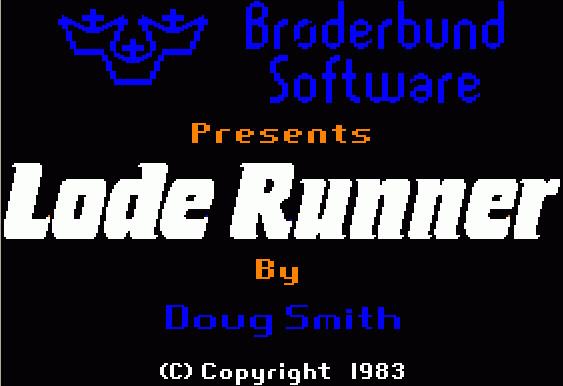
\includegraphics[width=\columnwidth]{title-screen}
\end{center}

You control the movement of your character, moving left and right along brick
and bedrock platforms, climbing ladders,
and "monkey-traversing" ropes strung across gaps. The object is to collect all the
gold boxes while avoiding being touched by the guards. You can dig holes in
brick parts of the floor which can allow you to reach otherwise unreachable caverns,
and the holes can also trap the guards for a short while. Holes fill themselves in
after a short time period, and if you're in a hole when that happens, you lose
a life. However, if a guard is in the hole and the hole fills, the guard disappears and
reappears somewhere along the top of the screen.

You get points for collecting boxes and forcing guards to respawn. Once you collect
all the boxes, a ladder will appear leading out of the top of the screen. This
gets you to the next level, and play continues.

\begin{center}
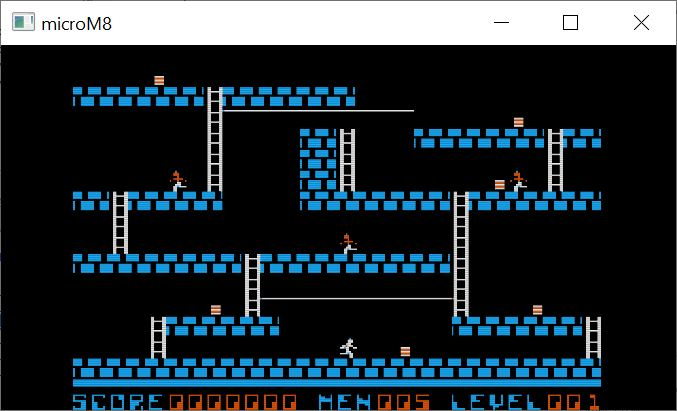
\includegraphics[width=\columnwidth]{screen}
\end{center}

Lode Runner included 150 levels and also a level editor.

\chapter{Apple II Graphics}
Hi-res graphics on the Apple II is odd. Graphics are memory-mapped, not exactly
consecutively, and bits don't always correspond to pixels. Color especially is
odd, compared to today's luxurious 32-bit per pixel RGBA.

The Apple II has two hi-res graphics pages, and maps the area from {\Tt{}{\$}2000-{\$}3FFF\nwendquote} to
high-res graphics page 1 (HGR1), and {\Tt{}{\$}4000-{\$}5FFF\nwendquote} to page 2 (HGR2).

We have routines to clear these screens.

\nwenddocs{}\nwbegincode{2}\sublabel{NW1Xx3lK-10jlgu-1}\nwmargintag{{\nwtagstyle{}\subpageref{NW1Xx3lK-10jlgu-1}}}\moddef{defines~{\nwtagstyle{}\subpageref{NW1Xx3lK-10jlgu-1}}}\endmoddef\nwstartdeflinemarkup\nwusesondefline{\\{NW1Xx3lK-1p0Y9w-1}}\nwprevnextdefs{\relax}{NW1Xx3lK-10jlgu-2}\nwenddeflinemarkup
    ORG     $0A
\nwlinkedidentc{TMP_PTR}{NW1Xx3lK-10jlgu-1}         DS.W    1
\nwindexdefn{\nwixident{TMP{\_}PTR}}{TMP:unPTR}{NW1Xx3lK-10jlgu-1}\eatline
\nwalsodefined{\\{NW1Xx3lK-10jlgu-2}\\{NW1Xx3lK-10jlgu-3}\\{NW1Xx3lK-10jlgu-4}\\{NW1Xx3lK-10jlgu-5}\\{NW1Xx3lK-10jlgu-6}\\{NW1Xx3lK-10jlgu-7}\\{NW1Xx3lK-10jlgu-8}\\{NW1Xx3lK-10jlgu-9}\\{NW1Xx3lK-10jlgu-A}\\{NW1Xx3lK-10jlgu-B}\\{NW1Xx3lK-10jlgu-C}\\{NW1Xx3lK-10jlgu-D}\\{NW1Xx3lK-10jlgu-E}\\{NW1Xx3lK-10jlgu-F}\\{NW1Xx3lK-10jlgu-G}\\{NW1Xx3lK-10jlgu-H}}\nwused{\\{NW1Xx3lK-1p0Y9w-1}}\nwidentdefs{\\{{\nwixident{TMP{\_}PTR}}{TMP:unPTR}}}\nwendcode{}\nwbegindocs{3}\nwdocspar
\nwenddocs{}\nwbegincode{4}\sublabel{NW1Xx3lK-8jv1b-1}\nwmargintag{{\nwtagstyle{}\subpageref{NW1Xx3lK-8jv1b-1}}}\moddef{routines~{\nwtagstyle{}\subpageref{NW1Xx3lK-8jv1b-1}}}\endmoddef\nwstartdeflinemarkup\nwusesondefline{\\{NW1Xx3lK-1p0Y9w-1}}\nwprevnextdefs{\relax}{NW1Xx3lK-8jv1b-2}\nwenddeflinemarkup
    ORG     $7A51
\nwlinkedidentc{CLEAR_HGR1}{NW1Xx3lK-8jv1b-1}:
    SUBROUTINE

    LDA     #$20                ; Start at $2000
    LDX     #$40                ; End at $4000 (but not including)
    BNE     CLEAR_PAGE          ; Unconditional jump

\nwlinkedidentc{CLEAR_HGR2}{NW1Xx3lK-8jv1b-1}:
    SUBROUTINE

    LDA     #$40                ; Start at $4000
    LDX     #$60                ; End at $6000 (but not including)
    ; fallthrough

CLEAR_PAGE:
    STA     \nwlinkedidentc{TMP_PTR}{NW1Xx3lK-10jlgu-1}+1           ; Start with the page in A.
    LDA     #$00
    STA     \nwlinkedidentc{TMP_PTR}{NW1Xx3lK-10jlgu-1}
    TAY
    LDA     #$80                ; fill byte = 0x80

.loop:
    STA     (\nwlinkedidentc{TMP_PTR}{NW1Xx3lK-10jlgu-1}),Y
    INY
    BNE     .loop
    INC     \nwlinkedidentc{TMP_PTR}{NW1Xx3lK-10jlgu-1}+1
    CPX     \nwlinkedidentc{TMP_PTR}{NW1Xx3lK-10jlgu-1}+1
    BNE     .loop               ; while \nwlinkedidentc{TMP_PTR}{NW1Xx3lK-10jlgu-1} != X * 0x100
    RTS
\nwindexdefn{\nwixident{CLEAR{\_}HGR1}}{CLEAR:unHGR1}{NW1Xx3lK-8jv1b-1}\nwindexdefn{\nwixident{CLEAR{\_}HGR2}}{CLEAR:unHGR2}{NW1Xx3lK-8jv1b-1}\eatline
\nwalsodefined{\\{NW1Xx3lK-8jv1b-2}\\{NW1Xx3lK-8jv1b-3}\\{NW1Xx3lK-8jv1b-4}\\{NW1Xx3lK-8jv1b-5}\\{NW1Xx3lK-8jv1b-6}\\{NW1Xx3lK-8jv1b-7}\\{NW1Xx3lK-8jv1b-8}\\{NW1Xx3lK-8jv1b-9}\\{NW1Xx3lK-8jv1b-A}\\{NW1Xx3lK-8jv1b-B}\\{NW1Xx3lK-8jv1b-C}\\{NW1Xx3lK-8jv1b-D}\\{NW1Xx3lK-8jv1b-E}\\{NW1Xx3lK-8jv1b-F}\\{NW1Xx3lK-8jv1b-G}\\{NW1Xx3lK-8jv1b-H}}\nwused{\\{NW1Xx3lK-1p0Y9w-1}}\nwidentdefs{\\{{\nwixident{CLEAR{\_}HGR1}}{CLEAR:unHGR1}}\\{{\nwixident{CLEAR{\_}HGR2}}{CLEAR:unHGR2}}}\nwidentuses{\\{{\nwixident{TMP{\_}PTR}}{TMP:unPTR}}}\nwindexuse{\nwixident{TMP{\_}PTR}}{TMP:unPTR}{NW1Xx3lK-8jv1b-1}\nwendcode{}\nwbegindocs{5}\nwdocspar
\section{Pixels and their color}
First we'll talk about pixels. Nominally, the resolution of the hi-res graphics screen
is 280 pixels wide by 192 pixels tall. In the memory map, each row is represented
by 40 bytes. The high bit of each byte is not used for pixel data, but is used to
control color.

Here are some rules for how these bytes are turned into pixels:
\begin{itemize}
  \item Pixels are drawn to the screen from byte data least significant bit first.
        This means that for the first byte bit 0 is column 0, bit 1 is column 1,
        and so on.
  \item A pattern of {\Tt{}11\nwendquote} results in two white pixels at the {\Tt{}1\nwendquote} positions.
  \item A pattern of {\Tt{}010\nwendquote} results at least in a colored pixel at the {\Tt{}1\nwendquote} position.
  \item A pattern of {\Tt{}101\nwendquote} results at least in a colored pixel at the {\Tt{}0\nwendquote} position.
  \item So, a pattern of {\Tt{}01010\nwendquote} results in at least three consecutive colored
        pixels starting from the first {\Tt{}1\nwendquote} to the last {\Tt{}1\nwendquote}. The last {\Tt{}0\nwendquote} bit
        would also be colored if followed by a {\Tt{}1\nwendquote}.
  \item Likewise, a pattern of {\Tt{}11011\nwendquote} results in two white pixels, a colored pixel,
        and then two more white pixels.
  \item The color of a {\Tt{}010\nwendquote} pixel depends on the column that the {\Tt{}1\nwendquote} falls on, and
        also whether the high bit of its byte was set or not. 
  \item The color of a {\Tt{}11011\nwendquote} pixel depends on the column that the {\Tt{}0\nwendquote} falls on, and
        also whether the high bit of its byte was set or not.

        \begin{center}
        \begin{tabular}{@{}rcc@{}} \toprule
        & Odd & Even \\ \cmidrule(r){2-3}
        High bit clear & Green & Violet \\
        High bit set & Orange & Blue \\ \bottomrule
        \end{tabular}
        \end{center}

        The implication is that you can only select one pair of colors per byte.
\end{itemize}

An example would probably be good here. We will take one of the sprites from the game.

\begin{center}
\begin{tabular}{@{}rcc@{}} \toprule
Bytes & Bits & Pixel Data \\ \cmidrule{1-3}
{\Tt{}00\ 00\nwendquote} & {\Tt{}0000000\ 0000000\nwendquote} & {\Tt{}00000000000000\nwendquote} \\
{\Tt{}00\ 00\nwendquote} & {\Tt{}0000000\ 0000000\nwendquote} & {\Tt{}00000000000000\nwendquote} \\
{\Tt{}00\ 00\nwendquote} & {\Tt{}0000000\ 0000000\nwendquote} & {\Tt{}00000000000000\nwendquote} \\
{\Tt{}55\ 00\nwendquote} & {\Tt{}1010101\ 0000000\nwendquote} & {\Tt{}10101010000000\nwendquote} \\
{\Tt{}41\ 00\nwendquote} & {\Tt{}1000001\ 0000000\nwendquote} & {\Tt{}10000010000000\nwendquote} \\
{\Tt{}01\ 00\nwendquote} & {\Tt{}0000001\ 0000000\nwendquote} & {\Tt{}10000000000000\nwendquote} \\
{\Tt{}55\ 00\nwendquote} & {\Tt{}1010101\ 0000000\nwendquote} & {\Tt{}10101010000000\nwendquote} \\
{\Tt{}50\ 00\nwendquote} & {\Tt{}1010000\ 0000000\nwendquote} & {\Tt{}00001010000000\nwendquote} \\
{\Tt{}50\ 00\nwendquote} & {\Tt{}1010000\ 0000000\nwendquote} & {\Tt{}00001010000000\nwendquote} \\
{\Tt{}51\ 00\nwendquote} & {\Tt{}1010001\ 0000000\nwendquote} & {\Tt{}10001010000000\nwendquote} \\
{\Tt{}55\ 00\nwendquote} & {\Tt{}1010101\ 0000000\nwendquote} & {\Tt{}10101010000000\nwendquote} \\ \bottomrule
\end{tabular}
\end{center}

The game automatically sets the high bit of each byte, so we know we're going to see
orange and blue. Assuming that the following bits are all zero, and we place the
sprite starting at column 0, we should see this:

\begin{center}
\begin{tabular}{@{}rcccccccccccccc@{}}
 0 & \bk0 & \bk0 & \bk0 & \bk0 & \bk0 & \bk0 & \bk0 & \bk0 & \bk0 & \bk0 & \bk0 & \bk0 & \bk0 & \bk0 \\
 1 & \bk0 & \bk0 & \bk0 & \bk0 & \bk0 & \bk0 & \bk0 & \bk0 & \bk0 & \bk0 & \bk0 & \bk0 & \bk0 & \bk0 \\
 2 & \bk0 & \bk0 & \bk0 & \bk0 & \bk0 & \bk0 & \bk0 & \bk0 & \bk0 & \bk0 & \bk0 & \bk0 & \bk0 & \bk0 \\
 3 & \bl0 & \bl0 & \bl0 & \bl0 & \bl0 & \bl0 & \bl0 & \bk0 & \bk0 & \bk0 & \bk0 & \bk0 & \bk0 & \bk0 \\
 4 & \bl0 & \bk0 & \bk0 & \bk0 & \bk0 & \bk0 & \bl0 & \bk0 & \bk0 & \bk0 & \bk0 & \bk0 & \bk0 & \bk0 \\
 5 & \bl0 & \bk0 & \bk0 & \bk0 & \bk0 & \bk0 & \bk0 & \bk0 & \bk0 & \bk0 & \bk0 & \bk0 & \bk0 & \bk0 \\
 6 & \bl0 & \bl0 & \bl0 & \bl0 & \bl0 & \bl0 & \bl0 & \bk0 & \bk0 & \bk0 & \bk0 & \bk0 & \bk0 & \bk0 \\
 7 & \bk0 & \bk0 & \bk0 & \bk0 & \bl0 & \bl0 & \bl0 & \bk0 & \bk0 & \bk0 & \bk0 & \bk0 & \bk0 & \bk0 \\
 8 & \bk0 & \bk0 & \bk0 & \bk0 & \bl0 & \bl0 & \bl0 & \bk0 & \bk0 & \bk0 & \bk0 & \bk0 & \bk0 & \bk0 \\
 9 & \bl0 & \bk0 & \bk0 & \bk0 & \bl0 & \bl0 & \bl0 & \bk0 & \bk0 & \bk0 & \bk0 & \bk0 & \bk0 & \bk0 \\
10 & \bl0 & \bl0 & \bl0 & \bl0 & \bl0 & \bl0 & \bl0 & \bk0 & \bk0 & \bk0 & \bk0 & \bk0 & \bk0 & \bk0 \\
\end{tabular}
\end{center}

Here is a more complex sprite:

\begin{center}
\begin{tabular}{@{}rcc@{}} \toprule
Bytes & Bits & Pixel Data \\ \cmidrule{1-3}
{\Tt{}40\ 00\nwendquote} & {\Tt{}1000000\ 0000000\nwendquote} & {\Tt{}00000010000000\nwendquote} \\
{\Tt{}60\ 01\nwendquote} & {\Tt{}1100000\ 0000001\nwendquote} & {\Tt{}00000111000000\nwendquote} \\
{\Tt{}60\ 01\nwendquote} & {\Tt{}1100000\ 0000001\nwendquote} & {\Tt{}00000111000000\nwendquote} \\
{\Tt{}70\ 00\nwendquote} & {\Tt{}1110000\ 0000000\nwendquote} & {\Tt{}00001110000000\nwendquote} \\
{\Tt{}6C\ 01\nwendquote} & {\Tt{}1101100\ 0000001\nwendquote} & {\Tt{}00110111000000\nwendquote} \\
{\Tt{}36\ 06\nwendquote} & {\Tt{}0110110\ 0000110\nwendquote} & {\Tt{}01101100110000\nwendquote} \\
{\Tt{}30\ 00\nwendquote} & {\Tt{}0110000\ 0000000\nwendquote} & {\Tt{}00001100000000\nwendquote} \\
{\Tt{}70\ 00\nwendquote} & {\Tt{}1110000\ 0000000\nwendquote} & {\Tt{}00001110000000\nwendquote} \\
{\Tt{}5E\ 01\nwendquote} & {\Tt{}1011110\ 0000001\nwendquote} & {\Tt{}01111011000000\nwendquote} \\
{\Tt{}40\ 01\nwendquote} & {\Tt{}1000000\ 0000001\nwendquote} & {\Tt{}00000011000000\nwendquote} \\
{\Tt{}40\ 01\nwendquote} & {\Tt{}1000000\ 0000001\nwendquote} & {\Tt{}00000011000000\nwendquote} \\ \bottomrule
\end{tabular}
\end{center}

\begin{center}
\begin{tabular}{@{}rcccccccccccccc@{}}
0 & \bk0 & \bk0 & \bk0 & \bk0 & \bk0 & \bk0 & \bl0 & \bk0 & \bk0 & \bk0 & \bk0 & \bk0 & \bk0 & \bk0 \\
1 & \bk0 & \bk0 & \bk0 & \bk0 & \bk0 & \bw0 & \bw0 & \bw0 & \bk0 & \bk0 & \bk0 & \bk0 & \bk0 & \bk0 \\
2 & \bk0 & \bk0 & \bk0 & \bk0 & \bk0 & \bw0 & \bw0 & \bw0 & \bk0 & \bk0 & \bk0 & \bk0 & \bk0 & \bk0 \\
3 & \bk0 & \bk0 & \bk0 & \bk0 & \bw0 & \bw0 & \bw0 & \bk0 & \bk0 & \bk0 & \bk0 & \bk0 & \bk0 & \bk0 \\
4 & \bk0 & \bk0 & \bw0 & \bw0 & \bo0 & \bw0 & \bw0 & \bw0 & \bk0 & \bk0 & \bk0 & \bk0 & \bk0 & \bk0 \\
5 & \bk0 & \bw0 & \bw0 & \bl0 & \bw0 & \bw0 & \bk0 & \bk0 & \bw0 & \bw0 & \bk0 & \bk0 & \bk0 & \bk0 \\
6 & \bk0 & \bk0 & \bk0 & \bk0 & \bw0 & \bw0 & \bk0 & \bk0 & \bk0 & \bk0 & \bk0 & \bk0 & \bk0 & \bk0 \\
7 & \bk0 & \bk0 & \bk0 & \bk0 & \bw0 & \bw0 & \bw0 & \bk0 & \bk0 & \bk0 & \bk0 & \bk0 & \bk0 & \bk0 \\
8 & \bk0 & \bw0 & \bw0 & \bw0 & \bw0 & \bl0 & \bw0 & \bw0 & \bk0 & \bk0 & \bk0 & \bk0 & \bk0 & \bk0 \\
9 & \bk0 & \bk0 & \bk0 & \bk0 & \bk0 & \bk0 & \bw0 & \bw0 & \bk0 & \bk0 & \bk0 & \bk0 & \bk0 & \bk0 \\
10 & \bk0 & \bk0 & \bk0 & \bk0 & \bk0 & \bk0 & \bw0 & \bw0 & \bk0 & \bk0 & \bk0 & \bk0 & \bk0 & \bk0 \\
\end{tabular}
\end{center}

Take note of the orange and blue pixels. All the patterns noted in the rules above are used.

\section{The sprites}
Lode Runner defines 104 sprites, each being 11 rows, with two bytes per row. The first bytes of
all 104 sprites are in the table first, then the second bytes, then the third bytes, and so on.
Later we will see that only the leftmost 10 pixels out of the 14-pixel description is used.

\nwenddocs{}\nwbegincode{6}\sublabel{NW1Xx3lK-1W8AJS-1}\nwmargintag{{\nwtagstyle{}\subpageref{NW1Xx3lK-1W8AJS-1}}}\moddef{tables~{\nwtagstyle{}\subpageref{NW1Xx3lK-1W8AJS-1}}}\endmoddef\nwstartdeflinemarkup\nwusesondefline{\\{NW1Xx3lK-1p0Y9w-1}}\nwprevnextdefs{\relax}{NW1Xx3lK-1W8AJS-2}\nwenddeflinemarkup
    ORG     $AD00
\nwlinkedidentc{SPRITE_DATA}{NW1Xx3lK-1W8AJS-1}:
    INCLUDE "sprite_data.asm"
\nwindexdefn{\nwixident{SPRITE{\_}DATA}}{SPRITE:unDATA}{NW1Xx3lK-1W8AJS-1}\eatline
\nwalsodefined{\\{NW1Xx3lK-1W8AJS-2}\\{NW1Xx3lK-1W8AJS-3}\\{NW1Xx3lK-1W8AJS-4}\\{NW1Xx3lK-1W8AJS-5}\\{NW1Xx3lK-1W8AJS-6}\\{NW1Xx3lK-1W8AJS-7}\\{NW1Xx3lK-1W8AJS-8}\\{NW1Xx3lK-1W8AJS-9}\\{NW1Xx3lK-1W8AJS-A}\\{NW1Xx3lK-1W8AJS-B}}\nwused{\\{NW1Xx3lK-1p0Y9w-1}}\nwidentdefs{\\{{\nwixident{SPRITE{\_}DATA}}{SPRITE:unDATA}}}\nwendcode{}\nwbegindocs{7}\nwdocspar
\begin{center}
\scalebox{0.8}{
\begin{tabular}{@{}rcccccccccccccccccccccccccccccc@{}}
 & \multicolumn{14}{c}{Sprite 0} & & \multicolumn{14}{c}{Sprite 1} \\
0 & \bk0 & \bk0 & \bk0 & \bk0 & \bk0 & \bk0 & \bk0 & \bk0 & \bk0 & \bk0 & \bk0 & \bk0 & \bk0 & \bk0 & & \bl0 & \bl0 & \bl0 & \bl0 & \bl0 & \bk0 & \bk0 & \bk0 & \bl0 & \bk0 & \bk0 & \bk0 & \bk0 & \bk0 & \\
1 & \bk0 & \bk0 & \bk0 & \bk0 & \bk0 & \bk0 & \bk0 & \bk0 & \bk0 & \bk0 & \bk0 & \bk0 & \bk0 & \bk0 & & \bl0 & \bl0 & \bl0 & \bl0 & \bl0 & \bk0 & \bk0 & \bk0 & \bl0 & \bk0 & \bk0 & \bk0 & \bk0 & \bk0 & \\
2 & \bk0 & \bk0 & \bk0 & \bk0 & \bk0 & \bk0 & \bk0 & \bk0 & \bk0 & \bk0 & \bk0 & \bk0 & \bk0 & \bk0 & & \bl0 & \bl0 & \bl0 & \bl0 & \bl0 & \bk0 & \bk0 & \bk0 & \bl0 & \bk0 & \bk0 & \bk0 & \bk0 & \bk0 & \\
3 & \bk0 & \bk0 & \bk0 & \bk0 & \bk0 & \bk0 & \bk0 & \bk0 & \bk0 & \bk0 & \bk0 & \bk0 & \bk0 & \bk0 & & \bl0 & \bl0 & \bl0 & \bl0 & \bl0 & \bk0 & \bk0 & \bk0 & \bl0 & \bk0 & \bk0 & \bk0 & \bk0 & \bk0 & \\
4 & \bk0 & \bk0 & \bk0 & \bk0 & \bk0 & \bk0 & \bk0 & \bk0 & \bk0 & \bk0 & \bk0 & \bk0 & \bk0 & \bk0 & & \bk0 & \bk0 & \bk0 & \bk0 & \bk0 & \bk0 & \bk0 & \bk0 & \bk0 & \bk0 & \bk0 & \bk0 & \bk0 & \bk0 & \\
5 & \bk0 & \bk0 & \bk0 & \bk0 & \bk0 & \bk0 & \bk0 & \bk0 & \bk0 & \bk0 & \bk0 & \bk0 & \bk0 & \bk0 & & \bl0 & \bk0 & \bk0 & \bk0 & \bl0 & \bl0 & \bl0 & \bl0 & \bl0 & \bk0 & \bk0 & \bk0 & \bk0 & \bk0 & \\
6 & \bk0 & \bk0 & \bk0 & \bk0 & \bk0 & \bk0 & \bk0 & \bk0 & \bk0 & \bk0 & \bk0 & \bk0 & \bk0 & \bk0 & & \bl0 & \bk0 & \bk0 & \bk0 & \bl0 & \bl0 & \bl0 & \bl0 & \bl0 & \bk0 & \bk0 & \bk0 & \bk0 & \bk0 & \\
7 & \bk0 & \bk0 & \bk0 & \bk0 & \bk0 & \bk0 & \bk0 & \bk0 & \bk0 & \bk0 & \bk0 & \bk0 & \bk0 & \bk0 & & \bl0 & \bk0 & \bk0 & \bk0 & \bl0 & \bl0 & \bl0 & \bl0 & \bl0 & \bk0 & \bk0 & \bk0 & \bk0 & \bk0 & \\
8 & \bk0 & \bk0 & \bk0 & \bk0 & \bk0 & \bk0 & \bk0 & \bk0 & \bk0 & \bk0 & \bk0 & \bk0 & \bk0 & \bk0 & & \bl0 & \bk0 & \bk0 & \bk0 & \bl0 & \bl0 & \bl0 & \bl0 & \bl0 & \bk0 & \bk0 & \bk0 & \bk0 & \bk0 & \\
9 & \bk0 & \bk0 & \bk0 & \bk0 & \bk0 & \bk0 & \bk0 & \bk0 & \bk0 & \bk0 & \bk0 & \bk0 & \bk0 & \bk0 & & \bl0 & \bk0 & \bk0 & \bk0 & \bl0 & \bl0 & \bl0 & \bl0 & \bl0 & \bk0 & \bk0 & \bk0 & \bk0 & \bk0 & \\
10 & \bk0 & \bk0 & \bk0 & \bk0 & \bk0 & \bk0 & \bk0 & \bk0 & \bk0 & \bk0 & \bk0 & \bk0 & \bk0 & \bk0 & & \bk0 & \bk0 & \bk0 & \bk0 & \bk0 & \bk0 & \bk0 & \bk0 & \bk0 & \bk0 & \bk0 & \bk0 & \bk0 & \bk0 & \\
\end{tabular}
}
\end{center}
\begin{center}
\scalebox{0.8}{
\begin{tabular}{@{}rcccccccccccccccccccccccccccccc@{}}
 & \multicolumn{14}{c}{Sprite 2} & & \multicolumn{14}{c}{Sprite 3} \\
0 & \bl0 & \bl0 & \bl0 & \bl0 & \bl0 & \bl0 & \bl0 & \bl0 & \bl0 & \bk0 & \bk0 & \bk0 & \bk0 & \bk0 & & \bk0 & \bw0 & \bw0 & \bk0 & \bk0 & \bk0 & \bk0 & \bw0 & \bw0 & \bk0 & \bk0 & \bk0 & \bk0 & \bk0 & \\
1 & \bl0 & \bl0 & \bl0 & \bl0 & \bl0 & \bl0 & \bl0 & \bl0 & \bl0 & \bk0 & \bk0 & \bk0 & \bk0 & \bk0 & & \bk0 & \bw0 & \bw0 & \bk0 & \bk0 & \bk0 & \bk0 & \bw0 & \bw0 & \bk0 & \bk0 & \bk0 & \bk0 & \bk0 & \\
2 & \bl0 & \bl0 & \bl0 & \bl0 & \bl0 & \bl0 & \bl0 & \bl0 & \bl0 & \bk0 & \bk0 & \bk0 & \bk0 & \bk0 & & \bk0 & \bw0 & \bw0 & \bw0 & \bw0 & \bw0 & \bw0 & \bw0 & \bw0 & \bk0 & \bk0 & \bk0 & \bk0 & \bk0 & \\
3 & \bl0 & \bl0 & \bl0 & \bl0 & \bl0 & \bl0 & \bl0 & \bl0 & \bl0 & \bk0 & \bk0 & \bk0 & \bk0 & \bk0 & & \bk0 & \bw0 & \bw0 & \bk0 & \bk0 & \bk0 & \bk0 & \bw0 & \bw0 & \bk0 & \bk0 & \bk0 & \bk0 & \bk0 & \\
4 & \bl0 & \bl0 & \bl0 & \bl0 & \bl0 & \bl0 & \bl0 & \bl0 & \bl0 & \bk0 & \bk0 & \bk0 & \bk0 & \bk0 & & \bk0 & \bw0 & \bw0 & \bk0 & \bk0 & \bk0 & \bk0 & \bw0 & \bw0 & \bk0 & \bk0 & \bk0 & \bk0 & \bk0 & \\
5 & \bl0 & \bl0 & \bl0 & \bl0 & \bl0 & \bl0 & \bl0 & \bl0 & \bl0 & \bk0 & \bk0 & \bk0 & \bk0 & \bk0 & & \bk0 & \bw0 & \bw0 & \bk0 & \bk0 & \bk0 & \bk0 & \bw0 & \bw0 & \bk0 & \bk0 & \bk0 & \bk0 & \bk0 & \\
6 & \bl0 & \bl0 & \bl0 & \bl0 & \bl0 & \bl0 & \bl0 & \bl0 & \bl0 & \bk0 & \bk0 & \bk0 & \bk0 & \bk0 & & \bk0 & \bw0 & \bw0 & \bk0 & \bk0 & \bk0 & \bk0 & \bw0 & \bw0 & \bk0 & \bk0 & \bk0 & \bk0 & \bk0 & \\
7 & \bl0 & \bl0 & \bl0 & \bl0 & \bl0 & \bl0 & \bl0 & \bl0 & \bl0 & \bk0 & \bk0 & \bk0 & \bk0 & \bk0 & & \bk0 & \bw0 & \bw0 & \bw0 & \bw0 & \bw0 & \bw0 & \bw0 & \bw0 & \bk0 & \bk0 & \bk0 & \bk0 & \bk0 & \\
8 & \bl0 & \bl0 & \bl0 & \bl0 & \bl0 & \bl0 & \bl0 & \bl0 & \bl0 & \bk0 & \bk0 & \bk0 & \bk0 & \bk0 & & \bk0 & \bw0 & \bw0 & \bk0 & \bk0 & \bk0 & \bk0 & \bw0 & \bw0 & \bk0 & \bk0 & \bk0 & \bk0 & \bk0 & \\
9 & \bl0 & \bl0 & \bl0 & \bl0 & \bl0 & \bl0 & \bl0 & \bl0 & \bl0 & \bk0 & \bk0 & \bk0 & \bk0 & \bk0 & & \bk0 & \bw0 & \bw0 & \bk0 & \bk0 & \bk0 & \bk0 & \bw0 & \bw0 & \bk0 & \bk0 & \bk0 & \bk0 & \bk0 & \\
10 & \bk0 & \bk0 & \bk0 & \bk0 & \bk0 & \bk0 & \bk0 & \bk0 & \bk0 & \bk0 & \bk0 & \bk0 & \bk0 & \bk0 & & \bk0 & \bw0 & \bw0 & \bk0 & \bk0 & \bk0 & \bk0 & \bw0 & \bw0 & \bk0 & \bk0 & \bk0 & \bk0 & \bk0 & \\
\end{tabular}
}
\end{center}
\begin{center}
\scalebox{0.8}{
\begin{tabular}{@{}rcccccccccccccccccccccccccccccc@{}}
 & \multicolumn{14}{c}{Sprite 4} & & \multicolumn{14}{c}{Sprite 5} \\
0 & \bk0 & \bk0 & \bk0 & \bk0 & \bk0 & \bk0 & \bk0 & \bk0 & \bk0 & \bk0 & \bk0 & \bk0 & \bk0 & \bk0 & & \bl0 & \bl0 & \bl0 & \bl0 & \bl0 & \bl0 & \bl0 & \bl0 & \bl0 & \bk0 & \bk0 & \bk0 & \bk0 & \bk0 & \\
1 & \bw0 & \bw0 & \bw0 & \bw0 & \bw0 & \bw0 & \bw0 & \bw0 & \bw0 & \bw0 & \bk0 & \bk0 & \bk0 & \bk0 & & \bl0 & \bl0 & \bl0 & \bl0 & \bl0 & \bl0 & \bl0 & \bl0 & \bl0 & \bk0 & \bk0 & \bk0 & \bk0 & \bk0 & \\
2 & \bk0 & \bk0 & \bk0 & \bk0 & \bk0 & \bk0 & \bk0 & \bk0 & \bk0 & \bk0 & \bk0 & \bk0 & \bk0 & \bk0 & & \bk0 & \bk0 & \bk0 & \bk0 & \bk0 & \bk0 & \bk0 & \bk0 & \bk0 & \bk0 & \bk0 & \bk0 & \bk0 & \bk0 & \\
3 & \bk0 & \bk0 & \bk0 & \bk0 & \bk0 & \bk0 & \bk0 & \bk0 & \bk0 & \bk0 & \bk0 & \bk0 & \bk0 & \bk0 & & \bk0 & \bk0 & \bw0 & \bw0 & \bw0 & \bw0 & \bw0 & \bw0 & \bk0 & \bk0 & \bk0 & \bk0 & \bk0 & \bk0 & \\
4 & \bk0 & \bk0 & \bk0 & \bk0 & \bk0 & \bk0 & \bk0 & \bk0 & \bk0 & \bk0 & \bk0 & \bk0 & \bk0 & \bk0 & & \bk0 & \bk0 & \bk0 & \bk0 & \bw0 & \bw0 & \bk0 & \bk0 & \bk0 & \bk0 & \bk0 & \bk0 & \bk0 & \bk0 & \\
5 & \bk0 & \bk0 & \bk0 & \bk0 & \bk0 & \bk0 & \bk0 & \bk0 & \bk0 & \bk0 & \bk0 & \bk0 & \bk0 & \bk0 & & \bk0 & \bk0 & \bk0 & \bk0 & \bw0 & \bw0 & \bk0 & \bk0 & \bk0 & \bk0 & \bk0 & \bk0 & \bk0 & \bk0 & \\
6 & \bk0 & \bk0 & \bk0 & \bk0 & \bk0 & \bk0 & \bk0 & \bk0 & \bk0 & \bk0 & \bk0 & \bk0 & \bk0 & \bk0 & & \bk0 & \bk0 & \bk0 & \bk0 & \bw0 & \bw0 & \bk0 & \bk0 & \bk0 & \bk0 & \bk0 & \bk0 & \bk0 & \bk0 & \\
7 & \bk0 & \bk0 & \bk0 & \bk0 & \bk0 & \bk0 & \bk0 & \bk0 & \bk0 & \bk0 & \bk0 & \bk0 & \bk0 & \bk0 & & \bk0 & \bk0 & \bk0 & \bk0 & \bw0 & \bw0 & \bk0 & \bk0 & \bk0 & \bk0 & \bk0 & \bk0 & \bk0 & \bk0 & \\
8 & \bk0 & \bk0 & \bk0 & \bk0 & \bk0 & \bk0 & \bk0 & \bk0 & \bk0 & \bk0 & \bk0 & \bk0 & \bk0 & \bk0 & & \bl0 & \bl0 & \bl0 & \bl0 & \bl0 & \bl0 & \bl0 & \bl0 & \bl0 & \bk0 & \bk0 & \bk0 & \bk0 & \bk0 & \\
9 & \bk0 & \bk0 & \bk0 & \bk0 & \bk0 & \bk0 & \bk0 & \bk0 & \bk0 & \bk0 & \bk0 & \bk0 & \bk0 & \bk0 & & \bl0 & \bl0 & \bl0 & \bl0 & \bl0 & \bl0 & \bl0 & \bl0 & \bl0 & \bk0 & \bk0 & \bk0 & \bk0 & \bk0 & \\
10 & \bk0 & \bk0 & \bk0 & \bk0 & \bk0 & \bk0 & \bk0 & \bk0 & \bk0 & \bk0 & \bk0 & \bk0 & \bk0 & \bk0 & & \bk0 & \bk0 & \bk0 & \bk0 & \bk0 & \bk0 & \bk0 & \bk0 & \bk0 & \bk0 & \bk0 & \bk0 & \bk0 & \bk0 & \\
\end{tabular}
}
\end{center}
\begin{center}
\scalebox{0.8}{
\begin{tabular}{@{}rcccccccccccccccccccccccccccccc@{}}
 & \multicolumn{14}{c}{Sprite 6} & & \multicolumn{14}{c}{Sprite 7} \\
0 & \bk0 & \bw0 & \bw0 & \bk0 & \bk0 & \bk0 & \bk0 & \bk0 & \bk0 & \bk0 & \bk0 & \bk0 & \bk0 & \bk0 & & \bk0 & \bk0 & \bk0 & \bk0 & \bk0 & \bk0 & \bk0 & \bk0 & \bk0 & \bk0 & \bk0 & \bk0 & \bk0 & \bk0 & \\
1 & \bk0 & \bw0 & \bw0 & \bk0 & \bk0 & \bk0 & \bk0 & \bk0 & \bk0 & \bk0 & \bk0 & \bk0 & \bk0 & \bk0 & & \bk0 & \bk0 & \bk0 & \bk0 & \bk0 & \bk0 & \bk0 & \bk0 & \bk0 & \bk0 & \bk0 & \bk0 & \bk0 & \bk0 & \\
2 & \bk0 & \bw0 & \bw0 & \bw0 & \bw0 & \bw0 & \bw0 & \bw0 & \bw0 & \bk0 & \bk0 & \bk0 & \bk0 & \bk0 & & \bk0 & \bk0 & \bk0 & \bk0 & \bk0 & \bk0 & \bk0 & \bk0 & \bk0 & \bk0 & \bk0 & \bk0 & \bk0 & \bk0 & \\
3 & \bk0 & \bw0 & \bw0 & \bk0 & \bk0 & \bk0 & \bk0 & \bw0 & \bw0 & \bk0 & \bk0 & \bk0 & \bk0 & \bk0 & & \bk0 & \bk0 & \bk0 & \bk0 & \bk0 & \bk0 & \bk0 & \bk0 & \bk0 & \bk0 & \bk0 & \bk0 & \bk0 & \bk0 & \\
4 & \bk0 & \bk0 & \bk0 & \bk0 & \bk0 & \bk0 & \bk0 & \bw0 & \bw0 & \bk0 & \bk0 & \bk0 & \bk0 & \bk0 & & \bk0 & \bk0 & \bk0 & \bk0 & \bk0 & \bk0 & \bk0 & \bk0 & \bk0 & \bk0 & \bk0 & \bk0 & \bk0 & \bk0 & \\
5 & \bk0 & \bk0 & \bk0 & \bk0 & \bk0 & \bk0 & \bk0 & \bw0 & \bw0 & \bk0 & \bk0 & \bk0 & \bk0 & \bk0 & & \bk0 & \bk0 & \bk0 & \bw0 & \bw0 & \bw0 & \bw0 & \bw0 & \bk0 & \bk0 & \bk0 & \bk0 & \bk0 & \bk0 & \\
6 & \bk0 & \bk0 & \bk0 & \bk0 & \bk0 & \bk0 & \bk0 & \bw0 & \bw0 & \bk0 & \bk0 & \bk0 & \bk0 & \bk0 & & \bk0 & \bk0 & \bk0 & \bo0 & \bo0 & \bo0 & \bo0 & \bo0 & \bk0 & \bk0 & \bk0 & \bk0 & \bk0 & \bk0 & \\
7 & \bk0 & \bw0 & \bw0 & \bk0 & \bk0 & \bk0 & \bk0 & \bw0 & \bw0 & \bk0 & \bk0 & \bk0 & \bk0 & \bk0 & & \bk0 & \bk0 & \bk0 & \bw0 & \bw0 & \bw0 & \bw0 & \bw0 & \bk0 & \bk0 & \bk0 & \bk0 & \bk0 & \bk0 & \\
8 & \bk0 & \bw0 & \bw0 & \bw0 & \bw0 & \bw0 & \bw0 & \bw0 & \bw0 & \bk0 & \bk0 & \bk0 & \bk0 & \bk0 & & \bk0 & \bk0 & \bk0 & \bo0 & \bo0 & \bo0 & \bo0 & \bo0 & \bk0 & \bk0 & \bk0 & \bk0 & \bk0 & \bk0 & \\
9 & \bk0 & \bw0 & \bw0 & \bk0 & \bk0 & \bk0 & \bk0 & \bk0 & \bk0 & \bk0 & \bk0 & \bk0 & \bk0 & \bk0 & & \bk0 & \bk0 & \bk0 & \bw0 & \bw0 & \bw0 & \bw0 & \bw0 & \bk0 & \bk0 & \bk0 & \bk0 & \bk0 & \bk0 & \\
10 & \bk0 & \bw0 & \bw0 & \bk0 & \bk0 & \bk0 & \bk0 & \bk0 & \bk0 & \bk0 & \bk0 & \bk0 & \bk0 & \bk0 & & \bk0 & \bk0 & \bk0 & \bk0 & \bk0 & \bk0 & \bk0 & \bk0 & \bk0 & \bk0 & \bk0 & \bk0 & \bk0 & \bk0 & \\
\end{tabular}
}
\end{center}
\begin{center}
\scalebox{0.8}{
\begin{tabular}{@{}rcccccccccccccccccccccccccccccc@{}}
 & \multicolumn{14}{c}{Sprite 8} & & \multicolumn{14}{c}{Sprite 9} \\
0 & \bk0 & \bk0 & \bk0 & \bk0 & \bl0 & \bk0 & \bk0 & \bk0 & \bk0 & \bk0 & \bk0 & \bk0 & \bk0 & \bk0 & & \bk0 & \bk0 & \bk0 & \bk0 & \bk0 & \bk0 & \bl0 & \bk0 & \bk0 & \bk0 & \bk0 & \bk0 & \bk0 & \bk0 & \\
1 & \bk0 & \bk0 & \bk0 & \bo0 & \bo0 & \bo0 & \bk0 & \bk0 & \bk0 & \bk0 & \bk0 & \bk0 & \bk0 & \bk0 & & \bk0 & \bk0 & \bk0 & \bk0 & \bk0 & \bw0 & \bw0 & \bw0 & \bk0 & \bk0 & \bk0 & \bk0 & \bk0 & \bk0 & \\
2 & \bk0 & \bk0 & \bk0 & \bo0 & \bo0 & \bo0 & \bk0 & \bk0 & \bk0 & \bk0 & \bk0 & \bk0 & \bk0 & \bk0 & & \bk0 & \bk0 & \bk0 & \bk0 & \bk0 & \bw0 & \bw0 & \bw0 & \bk0 & \bk0 & \bk0 & \bk0 & \bk0 & \bk0 & \\
3 & \bk0 & \bk0 & \bk0 & \bk0 & \bk0 & \bo0 & \bk0 & \bk0 & \bk0 & \bk0 & \bk0 & \bk0 & \bk0 & \bk0 & & \bk0 & \bk0 & \bk0 & \bk0 & \bw0 & \bw0 & \bw0 & \bk0 & \bk0 & \bk0 & \bk0 & \bk0 & \bk0 & \bk0 & \\
4 & \bk0 & \bk0 & \bk0 & \bo0 & \bo0 & \bo0 & \bo0 & \bo0 & \bk0 & \bk0 & \bk0 & \bk0 & \bk0 & \bk0 & & \bk0 & \bk0 & \bw0 & \bw0 & \bo0 & \bw0 & \bw0 & \bw0 & \bk0 & \bk0 & \bk0 & \bk0 & \bk0 & \bk0 & \\
5 & \bk0 & \bo0 & \bk0 & \bk0 & \bk0 & \bo0 & \bk0 & \bk0 & \bk0 & \bo0 & \bk0 & \bk0 & \bk0 & \bk0 & & \bk0 & \bw0 & \bw0 & \bl0 & \bw0 & \bw0 & \bk0 & \bk0 & \bw0 & \bw0 & \bk0 & \bk0 & \bk0 & \bk0 & \\
6 & \bk0 & \bk0 & \bk0 & \bk0 & \bk0 & \bw0 & \bw0 & \bk0 & \bk0 & \bk0 & \bk0 & \bk0 & \bk0 & \bk0 & & \bk0 & \bk0 & \bk0 & \bk0 & \bw0 & \bw0 & \bk0 & \bk0 & \bk0 & \bk0 & \bk0 & \bk0 & \bk0 & \bk0 & \\
7 & \bk0 & \bk0 & \bk0 & \bk0 & \bw0 & \bw0 & \bw0 & \bk0 & \bk0 & \bk0 & \bk0 & \bk0 & \bk0 & \bk0 & & \bk0 & \bk0 & \bk0 & \bk0 & \bw0 & \bw0 & \bw0 & \bk0 & \bk0 & \bk0 & \bk0 & \bk0 & \bk0 & \bk0 & \\
8 & \bk0 & \bk0 & \bk0 & \bw0 & \bw0 & \bl0 & \bw0 & \bw0 & \bw0 & \bw0 & \bk0 & \bk0 & \bk0 & \bk0 & & \bk0 & \bw0 & \bw0 & \bw0 & \bw0 & \bl0 & \bw0 & \bw0 & \bk0 & \bk0 & \bk0 & \bk0 & \bk0 & \bk0 & \\
9 & \bk0 & \bk0 & \bk0 & \bw0 & \bw0 & \bk0 & \bk0 & \bk0 & \bk0 & \bk0 & \bk0 & \bk0 & \bk0 & \bk0 & & \bk0 & \bk0 & \bk0 & \bk0 & \bk0 & \bk0 & \bw0 & \bw0 & \bk0 & \bk0 & \bk0 & \bk0 & \bk0 & \bk0 & \\
10 & \bk0 & \bk0 & \bk0 & \bw0 & \bw0 & \bk0 & \bk0 & \bk0 & \bk0 & \bk0 & \bk0 & \bk0 & \bk0 & \bk0 & & \bk0 & \bk0 & \bk0 & \bk0 & \bk0 & \bk0 & \bw0 & \bw0 & \bk0 & \bk0 & \bk0 & \bk0 & \bk0 & \bk0 & \\
\end{tabular}
}
\end{center}
\begin{center}
\scalebox{0.8}{
\begin{tabular}{@{}rcccccccccccccccccccccccccccccc@{}}
 & \multicolumn{14}{c}{Sprite 10} & & \multicolumn{14}{c}{Sprite 11} \\
0 & \bw0 & \bw0 & \bw0 & \bw0 & \bw0 & \bw0 & \bw0 & \bw0 & \bw0 & \bw0 & \bk0 & \bk0 & \bk0 & \bk0 & & \bk0 & \bk0 & \bk0 & \bo0 & \bk0 & \bk0 & \bk0 & \bk0 & \bk0 & \bk0 & \bk0 & \bk0 & \bk0 & \bk0 & \\
1 & \bw0 & \bw0 & \bw0 & \bw0 & \bw0 & \bw0 & \bw0 & \bw0 & \bw0 & \bw0 & \bk0 & \bk0 & \bk0 & \bk0 & & \bk0 & \bk0 & \bw0 & \bw0 & \bw0 & \bk0 & \bk0 & \bk0 & \bk0 & \bk0 & \bk0 & \bk0 & \bk0 & \bk0 & \\
2 & \bw0 & \bw0 & \bw0 & \bw0 & \bw0 & \bw0 & \bw0 & \bw0 & \bw0 & \bw0 & \bk0 & \bk0 & \bk0 & \bk0 & & \bk0 & \bk0 & \bw0 & \bw0 & \bw0 & \bk0 & \bk0 & \bk0 & \bk0 & \bk0 & \bk0 & \bk0 & \bk0 & \bk0 & \\
3 & \bw0 & \bw0 & \bw0 & \bw0 & \bw0 & \bw0 & \bw0 & \bw0 & \bw0 & \bw0 & \bk0 & \bk0 & \bk0 & \bk0 & & \bk0 & \bk0 & \bk0 & \bw0 & \bw0 & \bw0 & \bk0 & \bk0 & \bk0 & \bk0 & \bk0 & \bk0 & \bk0 & \bk0 & \\
4 & \bw0 & \bw0 & \bw0 & \bw0 & \bw0 & \bw0 & \bw0 & \bw0 & \bw0 & \bw0 & \bk0 & \bk0 & \bk0 & \bk0 & & \bk0 & \bk0 & \bw0 & \bw0 & \bw0 & \bl0 & \bw0 & \bw0 & \bk0 & \bk0 & \bk0 & \bk0 & \bk0 & \bk0 & \\
5 & \bw0 & \bw0 & \bw0 & \bw0 & \bw0 & \bw0 & \bw0 & \bw0 & \bw0 & \bw0 & \bk0 & \bk0 & \bk0 & \bk0 & & \bw0 & \bw0 & \bk0 & \bk0 & \bw0 & \bw0 & \bo0 & \bw0 & \bw0 & \bk0 & \bk0 & \bk0 & \bk0 & \bk0 & \\
6 & \bw0 & \bw0 & \bw0 & \bw0 & \bw0 & \bw0 & \bw0 & \bw0 & \bw0 & \bw0 & \bk0 & \bk0 & \bk0 & \bk0 & & \bk0 & \bk0 & \bk0 & \bk0 & \bw0 & \bw0 & \bk0 & \bk0 & \bk0 & \bk0 & \bk0 & \bk0 & \bk0 & \bk0 & \\
7 & \bw0 & \bw0 & \bw0 & \bw0 & \bw0 & \bw0 & \bw0 & \bw0 & \bw0 & \bw0 & \bk0 & \bk0 & \bk0 & \bk0 & & \bk0 & \bk0 & \bk0 & \bw0 & \bw0 & \bw0 & \bk0 & \bk0 & \bk0 & \bk0 & \bk0 & \bk0 & \bk0 & \bk0 & \\
8 & \bw0 & \bw0 & \bw0 & \bw0 & \bw0 & \bw0 & \bw0 & \bw0 & \bw0 & \bw0 & \bk0 & \bk0 & \bk0 & \bk0 & & \bk0 & \bk0 & \bw0 & \bw0 & \bo0 & \bw0 & \bw0 & \bw0 & \bw0 & \bk0 & \bk0 & \bk0 & \bk0 & \bk0 & \\
9 & \bw0 & \bw0 & \bw0 & \bw0 & \bw0 & \bw0 & \bw0 & \bw0 & \bw0 & \bw0 & \bk0 & \bk0 & \bk0 & \bk0 & & \bk0 & \bk0 & \bw0 & \bw0 & \bk0 & \bk0 & \bk0 & \bk0 & \bk0 & \bk0 & \bk0 & \bk0 & \bk0 & \bk0 & \\
10 & \bw0 & \bw0 & \bw0 & \bw0 & \bw0 & \bw0 & \bw0 & \bw0 & \bw0 & \bw0 & \bk0 & \bk0 & \bk0 & \bk0 & & \bk0 & \bk0 & \bw0 & \bw0 & \bk0 & \bk0 & \bk0 & \bk0 & \bk0 & \bk0 & \bk0 & \bk0 & \bk0 & \bk0 & \\
\end{tabular}
}
\end{center}
\begin{center}
\scalebox{0.8}{
\begin{tabular}{@{}rcccccccccccccccccccccccccccccc@{}}
 & \multicolumn{14}{c}{Sprite 12} & & \multicolumn{14}{c}{Sprite 13} \\
0 & \bk0 & \bk0 & \bk0 & \bo0 & \bk0 & \bk0 & \bk0 & \bk0 & \bk0 & \bk0 & \bk0 & \bk0 & \bk0 & \bk0 & & \bk0 & \bk0 & \bk0 & \bo0 & \bk0 & \bk0 & \bk0 & \bk0 & \bk0 & \bk0 & \bk0 & \bk0 & \bk0 & \bk0 & \\
1 & \bk0 & \bk0 & \bw0 & \bw0 & \bw0 & \bk0 & \bk0 & \bk0 & \bk0 & \bk0 & \bk0 & \bk0 & \bk0 & \bk0 & & \bk0 & \bk0 & \bw0 & \bw0 & \bw0 & \bk0 & \bk0 & \bk0 & \bk0 & \bk0 & \bk0 & \bk0 & \bk0 & \bk0 & \\
2 & \bk0 & \bk0 & \bw0 & \bw0 & \bw0 & \bk0 & \bk0 & \bk0 & \bk0 & \bk0 & \bk0 & \bk0 & \bk0 & \bk0 & & \bk0 & \bk0 & \bw0 & \bw0 & \bw0 & \bk0 & \bk0 & \bk0 & \bk0 & \bk0 & \bk0 & \bk0 & \bk0 & \bk0 & \\
3 & \bk0 & \bk0 & \bk0 & \bw0 & \bw0 & \bk0 & \bk0 & \bk0 & \bk0 & \bk0 & \bk0 & \bk0 & \bk0 & \bk0 & & \bk0 & \bk0 & \bk0 & \bw0 & \bw0 & \bk0 & \bk0 & \bk0 & \bk0 & \bk0 & \bk0 & \bk0 & \bk0 & \bk0 & \\
4 & \bk0 & \bk0 & \bk0 & \bw0 & \bw0 & \bw0 & \bk0 & \bk0 & \bk0 & \bk0 & \bk0 & \bk0 & \bk0 & \bk0 & & \bk0 & \bo0 & \bo0 & \bw0 & \bw0 & \bw0 & \bw0 & \bk0 & \bk0 & \bk0 & \bk0 & \bk0 & \bk0 & \bk0 & \\
5 & \bk0 & \bk0 & \bw0 & \bw0 & \bw0 & \bw0 & \bw0 & \bk0 & \bk0 & \bk0 & \bk0 & \bk0 & \bk0 & \bk0 & & \bk0 & \bw0 & \bw0 & \bw0 & \bw0 & \bl0 & \bw0 & \bw0 & \bk0 & \bk0 & \bk0 & \bk0 & \bk0 & \bk0 & \\
6 & \bw0 & \bw0 & \bo0 & \bw0 & \bw0 & \bw0 & \bw0 & \bk0 & \bk0 & \bk0 & \bk0 & \bk0 & \bk0 & \bk0 & & \bk0 & \bk0 & \bk0 & \bw0 & \bw0 & \bk0 & \bk0 & \bk0 & \bk0 & \bk0 & \bk0 & \bk0 & \bk0 & \bk0 & \\
7 & \bk0 & \bk0 & \bw0 & \bw0 & \bw0 & \bk0 & \bk0 & \bk0 & \bk0 & \bk0 & \bk0 & \bk0 & \bk0 & \bk0 & & \bk0 & \bk0 & \bw0 & \bw0 & \bw0 & \bw0 & \bk0 & \bk0 & \bk0 & \bk0 & \bk0 & \bk0 & \bk0 & \bk0 & \\
8 & \bk0 & \bk0 & \bw0 & \bw0 & \bw0 & \bw0 & \bk0 & \bk0 & \bk0 & \bk0 & \bk0 & \bk0 & \bk0 & \bk0 & & \bk0 & \bw0 & \bw0 & \bk0 & \bk0 & \bw0 & \bw0 & \bk0 & \bk0 & \bk0 & \bk0 & \bk0 & \bk0 & \bk0 & \\
9 & \bk0 & \bk0 & \bk0 & \bk0 & \bw0 & \bw0 & \bw0 & \bk0 & \bk0 & \bk0 & \bk0 & \bk0 & \bk0 & \bk0 & & \bk0 & \bw0 & \bw0 & \bk0 & \bk0 & \bk0 & \bw0 & \bw0 & \bk0 & \bk0 & \bk0 & \bk0 & \bk0 & \bk0 & \\
10 & \bk0 & \bk0 & \bk0 & \bk0 & \bw0 & \bw0 & \bk0 & \bk0 & \bk0 & \bk0 & \bk0 & \bk0 & \bk0 & \bk0 & & \bk0 & \bk0 & \bk0 & \bk0 & \bk0 & \bk0 & \bw0 & \bw0 & \bk0 & \bk0 & \bk0 & \bk0 & \bk0 & \bk0 & \\
\end{tabular}
}
\end{center}
\begin{center}
\scalebox{0.8}{
\begin{tabular}{@{}rcccccccccccccccccccccccccccccc@{}}
 & \multicolumn{14}{c}{Sprite 14} & & \multicolumn{14}{c}{Sprite 15} \\
0 & \bk0 & \bk0 & \bk0 & \bk0 & \bw0 & \bw0 & \bk0 & \bk0 & \bk0 & \bk0 & \bk0 & \bk0 & \bk0 & \bk0 & & \bk0 & \bk0 & \bk0 & \bk0 & \bk0 & \bk0 & \bl0 & \bk0 & \bk0 & \bk0 & \bk0 & \bk0 & \bk0 & \bk0 & \\
1 & \bk0 & \bk0 & \bk0 & \bk0 & \bw0 & \bw0 & \bk0 & \bk0 & \bk0 & \bo0 & \bk0 & \bk0 & \bk0 & \bk0 & & \bk0 & \bk0 & \bk0 & \bk0 & \bk0 & \bw0 & \bw0 & \bw0 & \bk0 & \bk0 & \bk0 & \bk0 & \bk0 & \bk0 & \\
2 & \bk0 & \bk0 & \bk0 & \bk0 & \bw0 & \bw0 & \bw0 & \bw0 & \bw0 & \bw0 & \bk0 & \bk0 & \bk0 & \bk0 & & \bk0 & \bk0 & \bk0 & \bk0 & \bk0 & \bw0 & \bw0 & \bw0 & \bk0 & \bk0 & \bk0 & \bk0 & \bk0 & \bk0 & \\
3 & \bk0 & \bo0 & \bk0 & \bk0 & \bw0 & \bw0 & \bw0 & \bk0 & \bk0 & \bk0 & \bk0 & \bk0 & \bk0 & \bk0 & & \bk0 & \bk0 & \bk0 & \bk0 & \bk0 & \bk0 & \bw0 & \bw0 & \bk0 & \bk0 & \bk0 & \bk0 & \bk0 & \bk0 & \\
4 & \bk0 & \bw0 & \bw0 & \bw0 & \bw0 & \bw0 & \bw0 & \bk0 & \bk0 & \bk0 & \bk0 & \bk0 & \bk0 & \bk0 & & \bk0 & \bk0 & \bk0 & \bk0 & \bw0 & \bw0 & \bw0 & \bw0 & \bw0 & \bw0 & \bk0 & \bk0 & \bk0 & \bk0 & \\
5 & \bk0 & \bk0 & \bk0 & \bk0 & \bw0 & \bw0 & \bw0 & \bk0 & \bk0 & \bk0 & \bk0 & \bk0 & \bk0 & \bk0 & & \bk0 & \bo0 & \bo0 & \bw0 & \bw0 & \bl0 & \bw0 & \bw0 & \bo0 & \bo0 & \bk0 & \bk0 & \bk0 & \bk0 & \\
6 & \bk0 & \bk0 & \bk0 & \bk0 & \bw0 & \bw0 & \bw0 & \bk0 & \bk0 & \bk0 & \bk0 & \bk0 & \bk0 & \bk0 & & \bk0 & \bo0 & \bk0 & \bk0 & \bk0 & \bk0 & \bw0 & \bw0 & \bk0 & \bk0 & \bk0 & \bk0 & \bk0 & \bk0 & \\
7 & \bk0 & \bk0 & \bk0 & \bw0 & \bw0 & \bl0 & \bw0 & \bw0 & \bk0 & \bk0 & \bk0 & \bk0 & \bk0 & \bk0 & & \bk0 & \bk0 & \bk0 & \bk0 & \bk0 & \bw0 & \bw0 & \bw0 & \bk0 & \bk0 & \bk0 & \bk0 & \bk0 & \bk0 & \\
8 & \bk0 & \bk0 & \bk0 & \bw0 & \bw0 & \bl0 & \bw0 & \bw0 & \bw0 & \bk0 & \bk0 & \bk0 & \bk0 & \bk0 & & \bk0 & \bk0 & \bk0 & \bk0 & \bw0 & \bw0 & \bo0 & \bw0 & \bw0 & \bk0 & \bk0 & \bk0 & \bk0 & \bk0 & \\
9 & \bk0 & \bk0 & \bk0 & \bw0 & \bw0 & \bk0 & \bk0 & \bk0 & \bk0 & \bk0 & \bk0 & \bk0 & \bk0 & \bk0 & & \bk0 & \bk0 & \bk0 & \bk0 & \bw0 & \bw0 & \bo0 & \bw0 & \bw0 & \bk0 & \bk0 & \bk0 & \bk0 & \bk0 & \\
10 & \bk0 & \bk0 & \bw0 & \bw0 & \bw0 & \bk0 & \bk0 & \bk0 & \bk0 & \bk0 & \bk0 & \bk0 & \bk0 & \bk0 & & \bk0 & \bk0 & \bk0 & \bk0 & \bw0 & \bw0 & \bo0 & \bw0 & \bw0 & \bk0 & \bk0 & \bk0 & \bk0 & \bk0 & \\
\end{tabular}
}
\end{center}
\begin{center}
\scalebox{0.8}{
\begin{tabular}{@{}rcccccccccccccccccccccccccccccc@{}}
 & \multicolumn{14}{c}{Sprite 16} & & \multicolumn{14}{c}{Sprite 17} \\
0 & \bk0 & \bk0 & \bk0 & \bk0 & \bk0 & \bk0 & \bl0 & \bk0 & \bk0 & \bk0 & \bk0 & \bk0 & \bk0 & \bk0 & & \bk0 & \bk0 & \bk0 & \bk0 & \bk0 & \bk0 & \bl0 & \bk0 & \bk0 & \bk0 & \bk0 & \bk0 & \bk0 & \bk0 & \\
1 & \bk0 & \bk0 & \bk0 & \bk0 & \bk0 & \bw0 & \bw0 & \bw0 & \bk0 & \bk0 & \bk0 & \bk0 & \bk0 & \bk0 & & \bk0 & \bk0 & \bk0 & \bk0 & \bk0 & \bw0 & \bw0 & \bw0 & \bk0 & \bk0 & \bk0 & \bk0 & \bk0 & \bk0 & \\
2 & \bk0 & \bk0 & \bk0 & \bk0 & \bk0 & \bw0 & \bw0 & \bw0 & \bk0 & \bk0 & \bk0 & \bk0 & \bk0 & \bk0 & & \bk0 & \bk0 & \bk0 & \bk0 & \bk0 & \bw0 & \bw0 & \bw0 & \bk0 & \bk0 & \bk0 & \bk0 & \bk0 & \bk0 & \\
3 & \bk0 & \bk0 & \bk0 & \bk0 & \bk0 & \bw0 & \bw0 & \bk0 & \bk0 & \bk0 & \bk0 & \bk0 & \bk0 & \bk0 & & \bk0 & \bk0 & \bk0 & \bk0 & \bk0 & \bw0 & \bw0 & \bk0 & \bk0 & \bk0 & \bk0 & \bk0 & \bk0 & \bk0 & \\
4 & \bk0 & \bk0 & \bk0 & \bk0 & \bw0 & \bw0 & \bw0 & \bk0 & \bk0 & \bk0 & \bk0 & \bk0 & \bk0 & \bk0 & & \bk0 & \bk0 & \bk0 & \bw0 & \bw0 & \bw0 & \bw0 & \bl0 & \bl0 & \bk0 & \bk0 & \bk0 & \bk0 & \bk0 & \\
5 & \bk0 & \bk0 & \bk0 & \bw0 & \bw0 & \bw0 & \bw0 & \bw0 & \bk0 & \bk0 & \bk0 & \bk0 & \bk0 & \bk0 & & \bk0 & \bk0 & \bw0 & \bw0 & \bo0 & \bw0 & \bw0 & \bw0 & \bw0 & \bk0 & \bk0 & \bk0 & \bk0 & \bk0 & \\
6 & \bk0 & \bk0 & \bk0 & \bw0 & \bw0 & \bw0 & \bw0 & \bl0 & \bw0 & \bw0 & \bk0 & \bk0 & \bk0 & \bk0 & & \bk0 & \bk0 & \bk0 & \bk0 & \bk0 & \bw0 & \bw0 & \bk0 & \bk0 & \bk0 & \bk0 & \bk0 & \bk0 & \bk0 & \\
7 & \bk0 & \bk0 & \bk0 & \bk0 & \bk0 & \bw0 & \bw0 & \bw0 & \bk0 & \bk0 & \bk0 & \bk0 & \bk0 & \bk0 & & \bk0 & \bk0 & \bk0 & \bk0 & \bw0 & \bw0 & \bw0 & \bw0 & \bk0 & \bk0 & \bk0 & \bk0 & \bk0 & \bk0 & \\
8 & \bk0 & \bk0 & \bk0 & \bk0 & \bw0 & \bw0 & \bw0 & \bw0 & \bk0 & \bk0 & \bk0 & \bk0 & \bk0 & \bk0 & & \bk0 & \bk0 & \bk0 & \bw0 & \bw0 & \bk0 & \bk0 & \bw0 & \bw0 & \bk0 & \bk0 & \bk0 & \bk0 & \bk0 & \\
9 & \bk0 & \bk0 & \bk0 & \bw0 & \bw0 & \bw0 & \bk0 & \bk0 & \bk0 & \bk0 & \bk0 & \bk0 & \bk0 & \bk0 & & \bk0 & \bk0 & \bw0 & \bw0 & \bk0 & \bk0 & \bk0 & \bw0 & \bw0 & \bk0 & \bk0 & \bk0 & \bk0 & \bk0 & \\
10 & \bk0 & \bk0 & \bk0 & \bk0 & \bw0 & \bw0 & \bk0 & \bk0 & \bk0 & \bk0 & \bk0 & \bk0 & \bk0 & \bk0 & & \bk0 & \bk0 & \bw0 & \bw0 & \bk0 & \bk0 & \bk0 & \bk0 & \bk0 & \bk0 & \bk0 & \bk0 & \bk0 & \bk0 & \\
\end{tabular}
}
\end{center}
\begin{center}
\scalebox{0.8}{
\begin{tabular}{@{}rcccccccccccccccccccccccccccccc@{}}
 & \multicolumn{14}{c}{Sprite 18} & & \multicolumn{14}{c}{Sprite 19} \\
0 & \bk0 & \bk0 & \bk0 & \bk0 & \bw0 & \bw0 & \bk0 & \bk0 & \bk0 & \bk0 & \bk0 & \bk0 & \bk0 & \bk0 & & \bk0 & \bw0 & \bw0 & \bk0 & \bk0 & \bo0 & \bk0 & \bk0 & \bw0 & \bw0 & \bk0 & \bk0 & \bk0 & \bk0 & \\
1 & \bl0 & \bk0 & \bk0 & \bk0 & \bw0 & \bw0 & \bk0 & \bk0 & \bk0 & \bk0 & \bk0 & \bk0 & \bk0 & \bk0 & & \bk0 & \bw0 & \bw0 & \bl0 & \bw0 & \bw0 & \bw0 & \bl0 & \bw0 & \bw0 & \bk0 & \bk0 & \bk0 & \bk0 & \\
2 & \bw0 & \bw0 & \bw0 & \bw0 & \bw0 & \bw0 & \bk0 & \bk0 & \bk0 & \bk0 & \bk0 & \bk0 & \bk0 & \bk0 & & \bk0 & \bw0 & \bw0 & \bl0 & \bw0 & \bw0 & \bw0 & \bl0 & \bw0 & \bw0 & \bk0 & \bk0 & \bk0 & \bk0 & \\
3 & \bk0 & \bk0 & \bk0 & \bw0 & \bw0 & \bw0 & \bk0 & \bk0 & \bl0 & \bk0 & \bk0 & \bk0 & \bk0 & \bk0 & & \bk0 & \bk0 & \bw0 & \bw0 & \bw0 & \bw0 & \bw0 & \bw0 & \bw0 & \bk0 & \bk0 & \bk0 & \bk0 & \bk0 & \\
4 & \bk0 & \bk0 & \bk0 & \bw0 & \bw0 & \bw0 & \bw0 & \bw0 & \bw0 & \bk0 & \bk0 & \bk0 & \bk0 & \bk0 & & \bk0 & \bk0 & \bk0 & \bk0 & \bk0 & \bw0 & \bw0 & \bk0 & \bk0 & \bk0 & \bk0 & \bk0 & \bk0 & \bk0 & \\
5 & \bk0 & \bk0 & \bk0 & \bw0 & \bw0 & \bw0 & \bk0 & \bk0 & \bk0 & \bk0 & \bk0 & \bk0 & \bk0 & \bk0 & & \bk0 & \bk0 & \bk0 & \bk0 & \bk0 & \bw0 & \bw0 & \bk0 & \bk0 & \bk0 & \bk0 & \bk0 & \bk0 & \bk0 & \\
6 & \bk0 & \bk0 & \bk0 & \bw0 & \bw0 & \bw0 & \bk0 & \bk0 & \bk0 & \bk0 & \bk0 & \bk0 & \bk0 & \bk0 & & \bk0 & \bk0 & \bk0 & \bw0 & \bw0 & \bw0 & \bw0 & \bk0 & \bk0 & \bk0 & \bk0 & \bk0 & \bk0 & \bk0 & \\
7 & \bk0 & \bk0 & \bw0 & \bw0 & \bo0 & \bw0 & \bw0 & \bk0 & \bk0 & \bk0 & \bk0 & \bk0 & \bk0 & \bk0 & & \bk0 & \bk0 & \bw0 & \bw0 & \bo0 & \bw0 & \bw0 & \bk0 & \bk0 & \bk0 & \bk0 & \bk0 & \bk0 & \bk0 & \\
8 & \bk0 & \bw0 & \bw0 & \bw0 & \bo0 & \bw0 & \bw0 & \bk0 & \bk0 & \bk0 & \bk0 & \bk0 & \bk0 & \bk0 & & \bk0 & \bk0 & \bw0 & \bw0 & \bo0 & \bw0 & \bw0 & \bk0 & \bk0 & \bk0 & \bk0 & \bk0 & \bk0 & \bk0 & \\
9 & \bk0 & \bk0 & \bk0 & \bk0 & \bk0 & \bw0 & \bw0 & \bk0 & \bk0 & \bk0 & \bk0 & \bk0 & \bk0 & \bk0 & & \bk0 & \bk0 & \bw0 & \bw0 & \bo0 & \bw0 & \bw0 & \bk0 & \bk0 & \bk0 & \bk0 & \bk0 & \bk0 & \bk0 & \\
10 & \bk0 & \bk0 & \bk0 & \bk0 & \bk0 & \bw0 & \bw0 & \bw0 & \bk0 & \bk0 & \bk0 & \bk0 & \bk0 & \bk0 & & \bk0 & \bk0 & \bk0 & \bk0 & \bk0 & \bw0 & \bw0 & \bk0 & \bk0 & \bk0 & \bk0 & \bk0 & \bk0 & \bk0 & \\
\end{tabular}
}
\end{center}
\begin{center}
\scalebox{0.8}{
\begin{tabular}{@{}rcccccccccccccccccccccccccccccc@{}}
 & \multicolumn{14}{c}{Sprite 20} & & \multicolumn{14}{c}{Sprite 21} \\
0 & \bw0 & \bw0 & \bk0 & \bk0 & \bl0 & \bk0 & \bk0 & \bw0 & \bw0 & \bk0 & \bk0 & \bk0 & \bk0 & \bk0 & & \bk0 & \bw0 & \bw0 & \bk0 & \bk0 & \bk0 & \bk0 & \bw0 & \bw0 & \bk0 & \bk0 & \bk0 & \bk0 & \bk0 & \\
1 & \bw0 & \bw0 & \bo0 & \bw0 & \bw0 & \bw0 & \bo0 & \bw0 & \bw0 & \bk0 & \bk0 & \bk0 & \bk0 & \bk0 & & \bk0 & \bw0 & \bw0 & \bk0 & \bk0 & \bk0 & \bk0 & \bw0 & \bw0 & \bk0 & \bk0 & \bk0 & \bk0 & \bk0 & \\
2 & \bw0 & \bw0 & \bo0 & \bw0 & \bw0 & \bw0 & \bo0 & \bw0 & \bw0 & \bk0 & \bk0 & \bk0 & \bk0 & \bk0 & & \bk0 & \bw0 & \bw0 & \bl0 & \bw0 & \bw0 & \bo0 & \bw0 & \bw0 & \bk0 & \bk0 & \bk0 & \bk0 & \bk0 & \\
3 & \bk0 & \bw0 & \bw0 & \bw0 & \bw0 & \bw0 & \bw0 & \bw0 & \bk0 & \bk0 & \bk0 & \bk0 & \bk0 & \bk0 & & \bk0 & \bw0 & \bw0 & \bl0 & \bw0 & \bw0 & \bw0 & \bw0 & \bk0 & \bk0 & \bk0 & \bk0 & \bk0 & \bk0 & \\
4 & \bk0 & \bk0 & \bk0 & \bw0 & \bw0 & \bk0 & \bk0 & \bk0 & \bk0 & \bk0 & \bk0 & \bk0 & \bk0 & \bk0 & & \bk0 & \bk0 & \bw0 & \bw0 & \bw0 & \bw0 & \bk0 & \bk0 & \bk0 & \bk0 & \bk0 & \bk0 & \bk0 & \bk0 & \\
5 & \bk0 & \bk0 & \bk0 & \bw0 & \bw0 & \bk0 & \bk0 & \bk0 & \bk0 & \bk0 & \bk0 & \bk0 & \bk0 & \bk0 & & \bk0 & \bk0 & \bk0 & \bw0 & \bw0 & \bk0 & \bk0 & \bk0 & \bk0 & \bk0 & \bk0 & \bk0 & \bk0 & \bk0 & \\
6 & \bk0 & \bk0 & \bk0 & \bw0 & \bw0 & \bw0 & \bw0 & \bk0 & \bk0 & \bk0 & \bk0 & \bk0 & \bk0 & \bk0 & & \bk0 & \bk0 & \bk0 & \bw0 & \bw0 & \bk0 & \bk0 & \bk0 & \bk0 & \bk0 & \bk0 & \bk0 & \bk0 & \bk0 & \\
7 & \bk0 & \bk0 & \bk0 & \bw0 & \bw0 & \bl0 & \bw0 & \bw0 & \bk0 & \bk0 & \bk0 & \bk0 & \bk0 & \bk0 & & \bk0 & \bw0 & \bw0 & \bw0 & \bw0 & \bk0 & \bk0 & \bk0 & \bk0 & \bk0 & \bk0 & \bk0 & \bk0 & \bk0 & \\
8 & \bk0 & \bk0 & \bk0 & \bw0 & \bw0 & \bl0 & \bw0 & \bw0 & \bk0 & \bk0 & \bk0 & \bk0 & \bk0 & \bk0 & & \bw0 & \bw0 & \bk0 & \bk0 & \bl0 & \bk0 & \bk0 & \bk0 & \bk0 & \bk0 & \bk0 & \bk0 & \bk0 & \bk0 & \\
9 & \bk0 & \bk0 & \bk0 & \bw0 & \bw0 & \bl0 & \bw0 & \bw0 & \bk0 & \bk0 & \bk0 & \bk0 & \bk0 & \bk0 & & \bw0 & \bw0 & \bo0 & \bw0 & \bw0 & \bk0 & \bk0 & \bk0 & \bk0 & \bk0 & \bk0 & \bk0 & \bk0 & \bk0 & \\
10 & \bk0 & \bk0 & \bk0 & \bw0 & \bw0 & \bk0 & \bk0 & \bk0 & \bk0 & \bk0 & \bk0 & \bk0 & \bk0 & \bk0 & & \bl0 & \bl0 & \bw0 & \bw0 & \bk0 & \bk0 & \bk0 & \bk0 & \bk0 & \bk0 & \bk0 & \bk0 & \bk0 & \bk0 & \\
\end{tabular}
}
\end{center}
\begin{center}
\scalebox{0.8}{
\begin{tabular}{@{}rcccccccccccccccccccccccccccccc@{}}
 & \multicolumn{14}{c}{Sprite 22} & & \multicolumn{14}{c}{Sprite 23} \\
0 & \bk0 & \bk0 & \bk0 & \bk0 & \bk0 & \bw0 & \bw0 & \bk0 & \bk0 & \bk0 & \bk0 & \bk0 & \bk0 & \bk0 & & \bk0 & \bk0 & \bk0 & \bw0 & \bw0 & \bk0 & \bk0 & \bk0 & \bk0 & \bk0 & \bk0 & \bk0 & \bk0 & \bk0 & \\
1 & \bk0 & \bk0 & \bk0 & \bk0 & \bk0 & \bw0 & \bw0 & \bk0 & \bk0 & \bk0 & \bk0 & \bk0 & \bk0 & \bk0 & & \bk0 & \bk0 & \bk0 & \bw0 & \bw0 & \bk0 & \bk0 & \bk0 & \bk0 & \bk0 & \bk0 & \bk0 & \bk0 & \bk0 & \\
2 & \bk0 & \bk0 & \bk0 & \bw0 & \bw0 & \bw0 & \bw0 & \bk0 & \bk0 & \bk0 & \bk0 & \bk0 & \bk0 & \bk0 & & \bk0 & \bk0 & \bk0 & \bw0 & \bw0 & \bw0 & \bw0 & \bk0 & \bk0 & \bk0 & \bk0 & \bk0 & \bk0 & \bk0 & \\
3 & \bk0 & \bk0 & \bk0 & \bw0 & \bw0 & \bw0 & \bk0 & \bk0 & \bk0 & \bk0 & \bk0 & \bk0 & \bk0 & \bk0 & & \bk0 & \bk0 & \bk0 & \bk0 & \bw0 & \bw0 & \bw0 & \bl0 & \bw0 & \bw0 & \bk0 & \bk0 & \bk0 & \bk0 & \\
4 & \bk0 & \bw0 & \bw0 & \bw0 & \bw0 & \bk0 & \bk0 & \bk0 & \bk0 & \bk0 & \bk0 & \bk0 & \bk0 & \bk0 & & \bk0 & \bk0 & \bk0 & \bk0 & \bk0 & \bw0 & \bw0 & \bw0 & \bw0 & \bk0 & \bk0 & \bk0 & \bk0 & \bk0 & \\
5 & \bw0 & \bw0 & \bo0 & \bw0 & \bw0 & \bk0 & \bk0 & \bk0 & \bk0 & \bk0 & \bk0 & \bk0 & \bk0 & \bk0 & & \bk0 & \bk0 & \bk0 & \bk0 & \bk0 & \bw0 & \bw0 & \bk0 & \bk0 & \bk0 & \bk0 & \bk0 & \bk0 & \bk0 & \\
6 & \bk0 & \bk0 & \bk0 & \bw0 & \bw0 & \bk0 & \bk0 & \bk0 & \bk0 & \bk0 & \bk0 & \bk0 & \bk0 & \bk0 & & \bk0 & \bk0 & \bk0 & \bk0 & \bk0 & \bw0 & \bw0 & \bk0 & \bk0 & \bk0 & \bk0 & \bk0 & \bk0 & \bk0 & \\
7 & \bk0 & \bk0 & \bw0 & \bw0 & \bw0 & \bk0 & \bk0 & \bk0 & \bk0 & \bk0 & \bk0 & \bk0 & \bk0 & \bk0 & & \bk0 & \bk0 & \bk0 & \bk0 & \bw0 & \bw0 & \bw0 & \bk0 & \bk0 & \bk0 & \bk0 & \bk0 & \bk0 & \bk0 & \\
8 & \bk0 & \bw0 & \bw0 & \bl0 & \bw0 & \bw0 & \bk0 & \bk0 & \bk0 & \bk0 & \bk0 & \bk0 & \bk0 & \bk0 & & \bk0 & \bk0 & \bk0 & \bw0 & \bw0 & \bl0 & \bw0 & \bw0 & \bk0 & \bk0 & \bk0 & \bk0 & \bk0 & \bk0 & \\
9 & \bk0 & \bw0 & \bw0 & \bl0 & \bw0 & \bw0 & \bk0 & \bk0 & \bk0 & \bk0 & \bk0 & \bk0 & \bk0 & \bk0 & & \bk0 & \bk0 & \bk0 & \bw0 & \bw0 & \bl0 & \bw0 & \bw0 & \bk0 & \bk0 & \bk0 & \bk0 & \bk0 & \bk0 & \\
10 & \bk0 & \bw0 & \bw0 & \bl0 & \bw0 & \bw0 & \bk0 & \bk0 & \bk0 & \bk0 & \bk0 & \bk0 & \bk0 & \bk0 & & \bk0 & \bk0 & \bk0 & \bw0 & \bw0 & \bl0 & \bw0 & \bw0 & \bk0 & \bk0 & \bk0 & \bk0 & \bk0 & \bk0 & \\
\end{tabular}
}
\end{center}
\begin{center}
\scalebox{0.8}{
\begin{tabular}{@{}rcccccccccccccccccccccccccccccc@{}}
 & \multicolumn{14}{c}{Sprite 24} & & \multicolumn{14}{c}{Sprite 25} \\
0 & \bk0 & \bw0 & \bw0 & \bk0 & \bk0 & \bk0 & \bk0 & \bw0 & \bw0 & \bk0 & \bk0 & \bk0 & \bk0 & \bk0 & & \bk0 & \bk0 & \bk0 & \bw0 & \bw0 & \bk0 & \bk0 & \bk0 & \bk0 & \bk0 & \bk0 & \bk0 & \bk0 & \bk0 & \\
1 & \bk0 & \bw0 & \bw0 & \bk0 & \bk0 & \bk0 & \bk0 & \bw0 & \bw0 & \bk0 & \bk0 & \bk0 & \bk0 & \bk0 & & \bk0 & \bk0 & \bk0 & \bw0 & \bw0 & \bk0 & \bk0 & \bk0 & \bk0 & \bk0 & \bk0 & \bk0 & \bk0 & \bk0 & \\
2 & \bk0 & \bw0 & \bw0 & \bl0 & \bw0 & \bw0 & \bo0 & \bw0 & \bw0 & \bk0 & \bk0 & \bk0 & \bk0 & \bk0 & & \bk0 & \bk0 & \bk0 & \bw0 & \bw0 & \bw0 & \bw0 & \bk0 & \bk0 & \bk0 & \bk0 & \bk0 & \bk0 & \bk0 & \\
3 & \bk0 & \bk0 & \bw0 & \bw0 & \bw0 & \bw0 & \bo0 & \bw0 & \bw0 & \bk0 & \bk0 & \bk0 & \bk0 & \bk0 & & \bk0 & \bk0 & \bk0 & \bk0 & \bw0 & \bw0 & \bw0 & \bk0 & \bk0 & \bk0 & \bk0 & \bk0 & \bk0 & \bk0 & \\
4 & \bk0 & \bk0 & \bk0 & \bk0 & \bw0 & \bw0 & \bw0 & \bw0 & \bk0 & \bk0 & \bk0 & \bk0 & \bk0 & \bk0 & & \bk0 & \bk0 & \bk0 & \bk0 & \bk0 & \bw0 & \bw0 & \bw0 & \bw0 & \bk0 & \bk0 & \bk0 & \bk0 & \bk0 & \\
5 & \bk0 & \bk0 & \bk0 & \bk0 & \bk0 & \bw0 & \bw0 & \bk0 & \bk0 & \bk0 & \bk0 & \bk0 & \bk0 & \bk0 & & \bk0 & \bk0 & \bk0 & \bk0 & \bk0 & \bw0 & \bw0 & \bl0 & \bw0 & \bw0 & \bk0 & \bk0 & \bk0 & \bk0 & \\
6 & \bk0 & \bk0 & \bk0 & \bk0 & \bk0 & \bw0 & \bw0 & \bk0 & \bk0 & \bk0 & \bk0 & \bk0 & \bk0 & \bk0 & & \bk0 & \bk0 & \bk0 & \bk0 & \bk0 & \bw0 & \bw0 & \bk0 & \bk0 & \bk0 & \bk0 & \bk0 & \bk0 & \bk0 & \\
7 & \bk0 & \bk0 & \bk0 & \bk0 & \bk0 & \bw0 & \bw0 & \bw0 & \bw0 & \bk0 & \bk0 & \bk0 & \bk0 & \bk0 & & \bk0 & \bk0 & \bk0 & \bk0 & \bk0 & \bw0 & \bw0 & \bw0 & \bk0 & \bk0 & \bk0 & \bk0 & \bk0 & \bk0 & \\
8 & \bk0 & \bk0 & \bk0 & \bk0 & \bk0 & \bo0 & \bk0 & \bk0 & \bw0 & \bw0 & \bk0 & \bk0 & \bk0 & \bk0 & & \bk0 & \bk0 & \bk0 & \bk0 & \bw0 & \bw0 & \bo0 & \bw0 & \bw0 & \bk0 & \bk0 & \bk0 & \bk0 & \bk0 & \\
9 & \bk0 & \bk0 & \bk0 & \bk0 & \bk0 & \bw0 & \bw0 & \bl0 & \bw0 & \bw0 & \bk0 & \bk0 & \bk0 & \bk0 & & \bk0 & \bk0 & \bk0 & \bk0 & \bw0 & \bw0 & \bo0 & \bw0 & \bw0 & \bk0 & \bk0 & \bk0 & \bk0 & \bk0 & \\
10 & \bk0 & \bk0 & \bk0 & \bk0 & \bk0 & \bk0 & \bw0 & \bw0 & \bo0 & \bo0 & \bk0 & \bk0 & \bk0 & \bk0 & & \bk0 & \bk0 & \bk0 & \bk0 & \bw0 & \bw0 & \bo0 & \bw0 & \bw0 & \bk0 & \bk0 & \bk0 & \bk0 & \bk0 & \\
\end{tabular}
}
\end{center}
\begin{center}
\scalebox{0.8}{
\begin{tabular}{@{}rcccccccccccccccccccccccccccccc@{}}
 & \multicolumn{14}{c}{Sprite 26} & & \multicolumn{14}{c}{Sprite 27} \\
0 & \bk0 & \bk0 & \bk0 & \bk0 & \bk0 & \bw0 & \bw0 & \bk0 & \bk0 & \bk0 & \bk0 & \bk0 & \bk0 & \bk0 & & \bk0 & \bk0 & \bk0 & \bk0 & \bk0 & \bk0 & \bk0 & \bk0 & \bk0 & \bk0 & \bk0 & \bk0 & \bk0 & \bk0 & \\
1 & \bk0 & \bk0 & \bk0 & \bk0 & \bk0 & \bw0 & \bw0 & \bk0 & \bk0 & \bk0 & \bk0 & \bk0 & \bk0 & \bk0 & & \bk0 & \bk0 & \bk0 & \bk0 & \bk0 & \bk0 & \bk0 & \bk0 & \bk0 & \bk0 & \bk0 & \bk0 & \bk0 & \bk0 & \\
2 & \bk0 & \bk0 & \bk0 & \bw0 & \bw0 & \bw0 & \bw0 & \bk0 & \bk0 & \bk0 & \bk0 & \bk0 & \bk0 & \bk0 & & \bk0 & \bk0 & \bk0 & \bk0 & \bk0 & \bk0 & \bk0 & \bk0 & \bk0 & \bk0 & \bk0 & \bk0 & \bk0 & \bk0 & \\
3 & \bw0 & \bw0 & \bo0 & \bw0 & \bw0 & \bw0 & \bk0 & \bk0 & \bk0 & \bk0 & \bk0 & \bk0 & \bk0 & \bk0 & & \bk0 & \bk0 & \bk0 & \bk0 & \bk0 & \bk0 & \bk0 & \bk0 & \bk0 & \bk0 & \bk0 & \bk0 & \bk0 & \bk0 & \\
4 & \bk0 & \bw0 & \bw0 & \bw0 & \bw0 & \bk0 & \bk0 & \bk0 & \bk0 & \bk0 & \bk0 & \bk0 & \bk0 & \bk0 & & \bk0 & \bk0 & \bk0 & \bk0 & \bk0 & \bk0 & \bk0 & \bk0 & \bk0 & \bk0 & \bk0 & \bk0 & \bk0 & \bk0 & \\
5 & \bk0 & \bk0 & \bk0 & \bw0 & \bw0 & \bk0 & \bk0 & \bk0 & \bk0 & \bk0 & \bk0 & \bk0 & \bk0 & \bk0 & & \bk0 & \bk0 & \bk0 & \bk0 & \bk0 & \bk0 & \bk0 & \bk0 & \bk0 & \bk0 & \bk0 & \bk0 & \bk0 & \bk0 & \\
6 & \bk0 & \bk0 & \bk0 & \bw0 & \bw0 & \bk0 & \bk0 & \bk0 & \bk0 & \bk0 & \bk0 & \bk0 & \bk0 & \bk0 & & \bk0 & \bk0 & \bk0 & \bk0 & \bl0 & \bk0 & \bk0 & \bk0 & \bk0 & \bk0 & \bk0 & \bk0 & \bk0 & \bk0 & \\
7 & \bk0 & \bk0 & \bk0 & \bw0 & \bw0 & \bw0 & \bk0 & \bk0 & \bk0 & \bk0 & \bk0 & \bk0 & \bk0 & \bk0 & & \bk0 & \bk0 & \bk0 & \bk0 & \bk0 & \bk0 & \bl0 & \bk0 & \bk0 & \bo0 & \bk0 & \bk0 & \bk0 & \bk0 & \\
8 & \bk0 & \bk0 & \bw0 & \bw0 & \bo0 & \bw0 & \bw0 & \bk0 & \bk0 & \bk0 & \bk0 & \bk0 & \bk0 & \bk0 & & \bk0 & \bk0 & \bl0 & \bk0 & \bk0 & \bk0 & \bk0 & \bk0 & \bk0 & \bo0 & \bk0 & \bk0 & \bk0 & \bk0 & \\
9 & \bk0 & \bk0 & \bw0 & \bw0 & \bo0 & \bw0 & \bw0 & \bk0 & \bk0 & \bk0 & \bk0 & \bk0 & \bk0 & \bk0 & & \bk0 & \bk0 & \bk0 & \bk0 & \bl0 & \bk0 & \bk0 & \bo0 & \bk0 & \bk0 & \bk0 & \bk0 & \bk0 & \bk0 & \\
10 & \bk0 & \bk0 & \bw0 & \bw0 & \bo0 & \bw0 & \bw0 & \bk0 & \bk0 & \bk0 & \bk0 & \bk0 & \bk0 & \bk0 & & \bk0 & \bk0 & \bk0 & \bk0 & \bk0 & \bk0 & \bk0 & \bo0 & \bk0 & \bk0 & \bk0 & \bk0 & \bk0 & \bk0 & \\
\end{tabular}
}
\end{center}
\begin{center}
\scalebox{0.8}{
\begin{tabular}{@{}rcccccccccccccccccccccccccccccc@{}}
 & \multicolumn{14}{c}{Sprite 28} & & \multicolumn{14}{c}{Sprite 29} \\
0 & \bk0 & \bk0 & \bk0 & \bk0 & \bk0 & \bk0 & \bk0 & \bk0 & \bk0 & \bk0 & \bk0 & \bk0 & \bk0 & \bk0 & & \bk0 & \bk0 & \bk0 & \bk0 & \bl0 & \bk0 & \bk0 & \bk0 & \bk0 & \bk0 & \bk0 & \bk0 & \bk0 & \bk0 & \\
1 & \bk0 & \bk0 & \bk0 & \bk0 & \bk0 & \bk0 & \bk0 & \bk0 & \bk0 & \bk0 & \bk0 & \bk0 & \bk0 & \bk0 & & \bk0 & \bk0 & \bk0 & \bk0 & \bk0 & \bk0 & \bk0 & \bk0 & \bk0 & \bk0 & \bk0 & \bk0 & \bk0 & \bk0 & \\
2 & \bk0 & \bk0 & \bk0 & \bk0 & \bk0 & \bk0 & \bk0 & \bk0 & \bk0 & \bk0 & \bk0 & \bk0 & \bk0 & \bk0 & & \bk0 & \bk0 & \bk0 & \bk0 & \bk0 & \bk0 & \bk0 & \bk0 & \bk0 & \bk0 & \bk0 & \bk0 & \bk0 & \bk0 & \\
3 & \bk0 & \bk0 & \bk0 & \bk0 & \bl0 & \bk0 & \bk0 & \bk0 & \bk0 & \bk0 & \bk0 & \bk0 & \bk0 & \bk0 & & \bk0 & \bk0 & \bk0 & \bk0 & \bk0 & \bk0 & \bk0 & \bk0 & \bk0 & \bk0 & \bk0 & \bk0 & \bk0 & \bk0 & \\
4 & \bk0 & \bk0 & \bk0 & \bk0 & \bk0 & \bk0 & \bk0 & \bk0 & \bk0 & \bk0 & \bk0 & \bk0 & \bk0 & \bk0 & & \bk0 & \bk0 & \bk0 & \bk0 & \bk0 & \bk0 & \bk0 & \bk0 & \bk0 & \bk0 & \bk0 & \bk0 & \bk0 & \bk0 & \\
5 & \bk0 & \bk0 & \bk0 & \bk0 & \bk0 & \bk0 & \bk0 & \bk0 & \bl0 & \bk0 & \bk0 & \bk0 & \bk0 & \bk0 & & \bl0 & \bk0 & \bk0 & \bk0 & \bl0 & \bk0 & \bk0 & \bk0 & \bk0 & \bk0 & \bk0 & \bk0 & \bk0 & \bk0 & \\
6 & \bl0 & \bk0 & \bk0 & \bk0 & \bk0 & \bk0 & \bk0 & \bk0 & \bk0 & \bk0 & \bk0 & \bk0 & \bk0 & \bk0 & & \bk0 & \bk0 & \bk0 & \bk0 & \bk0 & \bk0 & \bk0 & \bk0 & \bl0 & \bk0 & \bk0 & \bk0 & \bk0 & \bk0 & \\
7 & \bk0 & \bk0 & \bl0 & \bk0 & \bk0 & \bk0 & \bk0 & \bk0 & \bk0 & \bk0 & \bk0 & \bk0 & \bk0 & \bk0 & & \bl0 & \bk0 & \bk0 & \bk0 & \bk0 & \bk0 & \bk0 & \bk0 & \bk0 & \bk0 & \bk0 & \bk0 & \bk0 & \bk0 & \\
8 & \bk0 & \bk0 & \bk0 & \bk0 & \bl0 & \bl0 & \bl0 & \bk0 & \bk0 & \bo0 & \bk0 & \bk0 & \bk0 & \bk0 & & \bk0 & \bk0 & \bl0 & \bk0 & \bk0 & \bk0 & \bk0 & \bk0 & \bk0 & \bk0 & \bk0 & \bk0 & \bk0 & \bk0 & \\
9 & \bk0 & \bk0 & \bl0 & \bk0 & \bk0 & \bk0 & \bk0 & \bo0 & \bo0 & \bo0 & \bk0 & \bk0 & \bk0 & \bk0 & & \bk0 & \bk0 & \bk0 & \bk0 & \bk0 & \bk0 & \bl0 & \bk0 & \bk0 & \bk0 & \bk0 & \bk0 & \bk0 & \bk0 & \\
10 & \bk0 & \bk0 & \bk0 & \bk0 & \bl0 & \bk0 & \bk0 & \bo0 & \bk0 & \bk0 & \bk0 & \bk0 & \bk0 & \bk0 & & \bk0 & \bk0 & \bk0 & \bk0 & \bk0 & \bk0 & \bk0 & \bk0 & \bk0 & \bk0 & \bk0 & \bk0 & \bk0 & \bk0 & \\
\end{tabular}
}
\end{center}
\begin{center}
\scalebox{0.8}{
\begin{tabular}{@{}rcccccccccccccccccccccccccccccc@{}}
 & \multicolumn{14}{c}{Sprite 30} & & \multicolumn{14}{c}{Sprite 31} \\
0 & \bk0 & \bk0 & \bk0 & \bk0 & \bk0 & \bk0 & \bk0 & \bk0 & \bk0 & \bk0 & \bk0 & \bk0 & \bk0 & \bk0 & & \bl0 & \bl0 & \bl0 & \bk0 & \bk0 & \bo0 & \bk0 & \bk0 & \bl0 & \bk0 & \bk0 & \bk0 & \bk0 & \bk0 & \\
1 & \bk0 & \bk0 & \bk0 & \bk0 & \bk0 & \bk0 & \bk0 & \bk0 & \bk0 & \bk0 & \bk0 & \bk0 & \bk0 & \bk0 & & \bl0 & \bl0 & \bl0 & \bl0 & \bl0 & \bk0 & \bk0 & \bk0 & \bl0 & \bk0 & \bk0 & \bk0 & \bk0 & \bk0 & \\
2 & \bk0 & \bk0 & \bk0 & \bk0 & \bk0 & \bk0 & \bk0 & \bk0 & \bk0 & \bk0 & \bk0 & \bk0 & \bk0 & \bk0 & & \bl0 & \bl0 & \bl0 & \bl0 & \bl0 & \bk0 & \bk0 & \bk0 & \bl0 & \bk0 & \bk0 & \bk0 & \bk0 & \bk0 & \\
3 & \bk0 & \bk0 & \bk0 & \bk0 & \bl0 & \bk0 & \bk0 & \bk0 & \bk0 & \bk0 & \bk0 & \bk0 & \bk0 & \bk0 & & \bl0 & \bl0 & \bl0 & \bl0 & \bl0 & \bk0 & \bk0 & \bk0 & \bl0 & \bk0 & \bk0 & \bk0 & \bk0 & \bk0 & \\
4 & \bk0 & \bk0 & \bk0 & \bk0 & \bk0 & \bk0 & \bk0 & \bk0 & \bk0 & \bk0 & \bk0 & \bk0 & \bk0 & \bk0 & & \bk0 & \bk0 & \bk0 & \bk0 & \bk0 & \bk0 & \bk0 & \bk0 & \bk0 & \bk0 & \bk0 & \bk0 & \bk0 & \bk0 & \\
5 & \bl0 & \bk0 & \bk0 & \bk0 & \bk0 & \bk0 & \bk0 & \bk0 & \bk0 & \bk0 & \bk0 & \bk0 & \bk0 & \bk0 & & \bl0 & \bk0 & \bk0 & \bk0 & \bl0 & \bl0 & \bl0 & \bl0 & \bl0 & \bk0 & \bk0 & \bk0 & \bk0 & \bk0 & \\
6 & \bk0 & \bk0 & \bk0 & \bk0 & \bk0 & \bk0 & \bk0 & \bk0 & \bk0 & \bk0 & \bk0 & \bk0 & \bk0 & \bk0 & & \bl0 & \bk0 & \bk0 & \bk0 & \bl0 & \bl0 & \bl0 & \bl0 & \bl0 & \bk0 & \bk0 & \bk0 & \bk0 & \bk0 & \\
7 & \bk0 & \bk0 & \bk0 & \bk0 & \bk0 & \bk0 & \bk0 & \bk0 & \bl0 & \bk0 & \bk0 & \bk0 & \bk0 & \bk0 & & \bl0 & \bk0 & \bk0 & \bk0 & \bl0 & \bl0 & \bl0 & \bl0 & \bl0 & \bk0 & \bk0 & \bk0 & \bk0 & \bk0 & \\
8 & \bk0 & \bk0 & \bk0 & \bk0 & \bk0 & \bk0 & \bk0 & \bk0 & \bk0 & \bk0 & \bk0 & \bk0 & \bk0 & \bk0 & & \bl0 & \bk0 & \bk0 & \bk0 & \bl0 & \bl0 & \bl0 & \bl0 & \bl0 & \bk0 & \bk0 & \bk0 & \bk0 & \bk0 & \\
9 & \bk0 & \bk0 & \bk0 & \bk0 & \bk0 & \bk0 & \bk0 & \bk0 & \bk0 & \bk0 & \bk0 & \bk0 & \bk0 & \bk0 & & \bl0 & \bk0 & \bk0 & \bk0 & \bl0 & \bl0 & \bl0 & \bl0 & \bl0 & \bk0 & \bk0 & \bk0 & \bk0 & \bk0 & \\
10 & \bk0 & \bk0 & \bk0 & \bk0 & \bk0 & \bk0 & \bk0 & \bk0 & \bk0 & \bk0 & \bk0 & \bk0 & \bk0 & \bk0 & & \bk0 & \bk0 & \bk0 & \bk0 & \bk0 & \bk0 & \bk0 & \bk0 & \bk0 & \bk0 & \bk0 & \bk0 & \bk0 & \bk0 & \\
\end{tabular}
}
\end{center}
\begin{center}
\scalebox{0.8}{
\begin{tabular}{@{}rcccccccccccccccccccccccccccccc@{}}
 & \multicolumn{14}{c}{Sprite 32} & & \multicolumn{14}{c}{Sprite 33} \\
0 & \bk0 & \bk0 & \bk0 & \bk0 & \bk0 & \bo0 & \bk0 & \bk0 & \bk0 & \bk0 & \bk0 & \bk0 & \bk0 & \bk0 & & \bk0 & \bk0 & \bk0 & \bk0 & \bk0 & \bk0 & \bk0 & \bk0 & \bk0 & \bk0 & \bk0 & \bk0 & \bk0 & \bk0 & \\
1 & \bk0 & \bk0 & \bk0 & \bo0 & \bo0 & \bo0 & \bk0 & \bk0 & \bk0 & \bk0 & \bk0 & \bk0 & \bk0 & \bk0 & & \bk0 & \bk0 & \bk0 & \bk0 & \bk0 & \bo0 & \bk0 & \bk0 & \bk0 & \bk0 & \bk0 & \bk0 & \bk0 & \bk0 & \\
2 & \bl0 & \bk0 & \bk0 & \bk0 & \bk0 & \bk0 & \bk0 & \bk0 & \bl0 & \bk0 & \bk0 & \bk0 & \bk0 & \bk0 & & \bk0 & \bk0 & \bk0 & \bo0 & \bo0 & \bo0 & \bk0 & \bk0 & \bk0 & \bk0 & \bk0 & \bk0 & \bk0 & \bk0 & \\
3 & \bl0 & \bl0 & \bl0 & \bl0 & \bl0 & \bk0 & \bk0 & \bk0 & \bl0 & \bk0 & \bk0 & \bk0 & \bk0 & \bk0 & & \bl0 & \bk0 & \bk0 & \bo0 & \bo0 & \bo0 & \bk0 & \bk0 & \bl0 & \bk0 & \bk0 & \bk0 & \bk0 & \bk0 & \\
4 & \bk0 & \bk0 & \bk0 & \bk0 & \bk0 & \bk0 & \bk0 & \bk0 & \bk0 & \bk0 & \bk0 & \bk0 & \bk0 & \bk0 & & \bk0 & \bk0 & \bk0 & \bk0 & \bk0 & \bk0 & \bk0 & \bk0 & \bk0 & \bk0 & \bk0 & \bk0 & \bk0 & \bk0 & \\
5 & \bl0 & \bk0 & \bk0 & \bk0 & \bl0 & \bl0 & \bl0 & \bl0 & \bl0 & \bk0 & \bk0 & \bk0 & \bk0 & \bk0 & & \bl0 & \bk0 & \bk0 & \bk0 & \bl0 & \bl0 & \bl0 & \bl0 & \bl0 & \bk0 & \bk0 & \bk0 & \bk0 & \bk0 & \\
6 & \bl0 & \bk0 & \bk0 & \bk0 & \bl0 & \bl0 & \bl0 & \bl0 & \bl0 & \bk0 & \bk0 & \bk0 & \bk0 & \bk0 & & \bl0 & \bk0 & \bk0 & \bk0 & \bl0 & \bl0 & \bl0 & \bl0 & \bl0 & \bk0 & \bk0 & \bk0 & \bk0 & \bk0 & \\
7 & \bl0 & \bk0 & \bk0 & \bk0 & \bl0 & \bl0 & \bl0 & \bl0 & \bl0 & \bk0 & \bk0 & \bk0 & \bk0 & \bk0 & & \bl0 & \bk0 & \bk0 & \bk0 & \bl0 & \bl0 & \bl0 & \bl0 & \bl0 & \bk0 & \bk0 & \bk0 & \bk0 & \bk0 & \\
8 & \bl0 & \bk0 & \bk0 & \bk0 & \bl0 & \bl0 & \bl0 & \bl0 & \bl0 & \bk0 & \bk0 & \bk0 & \bk0 & \bk0 & & \bl0 & \bk0 & \bk0 & \bk0 & \bl0 & \bl0 & \bl0 & \bl0 & \bl0 & \bk0 & \bk0 & \bk0 & \bk0 & \bk0 & \\
9 & \bl0 & \bk0 & \bk0 & \bk0 & \bl0 & \bl0 & \bl0 & \bl0 & \bl0 & \bk0 & \bk0 & \bk0 & \bk0 & \bk0 & & \bl0 & \bk0 & \bk0 & \bk0 & \bl0 & \bl0 & \bl0 & \bl0 & \bl0 & \bk0 & \bk0 & \bk0 & \bk0 & \bk0 & \\
10 & \bk0 & \bk0 & \bk0 & \bk0 & \bk0 & \bk0 & \bk0 & \bk0 & \bk0 & \bk0 & \bk0 & \bk0 & \bk0 & \bk0 & & \bk0 & \bk0 & \bk0 & \bk0 & \bk0 & \bk0 & \bk0 & \bk0 & \bk0 & \bk0 & \bk0 & \bk0 & \bk0 & \bk0 & \\
\end{tabular}
}
\end{center}
\begin{center}
\scalebox{0.8}{
\begin{tabular}{@{}rcccccccccccccccccccccccccccccc@{}}
 & \multicolumn{14}{c}{Sprite 34} & & \multicolumn{14}{c}{Sprite 35} \\
0 & \bk0 & \bk0 & \bk0 & \bk0 & \bk0 & \bk0 & \bk0 & \bk0 & \bk0 & \bk0 & \bk0 & \bk0 & \bk0 & \bk0 & & \bk0 & \bk0 & \bk0 & \bk0 & \bk0 & \bk0 & \bk0 & \bk0 & \bk0 & \bk0 & \bk0 & \bk0 & \bk0 & \bk0 & \\
1 & \bk0 & \bk0 & \bk0 & \bk0 & \bk0 & \bk0 & \bk0 & \bk0 & \bk0 & \bk0 & \bk0 & \bk0 & \bk0 & \bk0 & & \bk0 & \bk0 & \bk0 & \bk0 & \bk0 & \bk0 & \bk0 & \bk0 & \bk0 & \bk0 & \bk0 & \bk0 & \bk0 & \bk0 & \\
2 & \bk0 & \bk0 & \bk0 & \bk0 & \bk0 & \bk0 & \bk0 & \bk0 & \bk0 & \bk0 & \bk0 & \bk0 & \bk0 & \bk0 & & \bk0 & \bk0 & \bk0 & \bk0 & \bk0 & \bk0 & \bk0 & \bk0 & \bk0 & \bk0 & \bk0 & \bk0 & \bk0 & \bk0 & \\
3 & \bk0 & \bk0 & \bk0 & \bk0 & \bk0 & \bo0 & \bk0 & \bk0 & \bk0 & \bk0 & \bk0 & \bk0 & \bk0 & \bk0 & & \bk0 & \bk0 & \bk0 & \bk0 & \bk0 & \bk0 & \bk0 & \bk0 & \bk0 & \bk0 & \bk0 & \bk0 & \bk0 & \bk0 & \\
4 & \bk0 & \bk0 & \bk0 & \bo0 & \bo0 & \bo0 & \bk0 & \bk0 & \bk0 & \bk0 & \bk0 & \bk0 & \bk0 & \bk0 & & \bk0 & \bk0 & \bk0 & \bk0 & \bk0 & \bk0 & \bk0 & \bk0 & \bk0 & \bk0 & \bk0 & \bk0 & \bk0 & \bk0 & \\
5 & \bk0 & \bk0 & \bk0 & \bo0 & \bo0 & \bo0 & \bo0 & \bo0 & \bk0 & \bk0 & \bk0 & \bk0 & \bk0 & \bk0 & & \bk0 & \bk0 & \bk0 & \bk0 & \bk0 & \bo0 & \bk0 & \bk0 & \bk0 & \bk0 & \bk0 & \bk0 & \bk0 & \bk0 & \\
6 & \bk0 & \bk0 & \bk0 & \bk0 & \bk0 & \bk0 & \bk0 & \bk0 & \bk0 & \bk0 & \bk0 & \bk0 & \bk0 & \bk0 & & \bk0 & \bk0 & \bk0 & \bk0 & \bk0 & \bo0 & \bo0 & \bo0 & \bk0 & \bk0 & \bk0 & \bk0 & \bk0 & \bk0 & \\
7 & \bl0 & \bk0 & \bk0 & \bk0 & \bl0 & \bl0 & \bl0 & \bl0 & \bl0 & \bk0 & \bk0 & \bk0 & \bk0 & \bk0 & & \bl0 & \bk0 & \bk0 & \bo0 & \bo0 & \bo0 & \bo0 & \bo0 & \bk0 & \bk0 & \bk0 & \bk0 & \bk0 & \bk0 & \\
8 & \bl0 & \bk0 & \bk0 & \bk0 & \bl0 & \bl0 & \bl0 & \bl0 & \bl0 & \bk0 & \bk0 & \bk0 & \bk0 & \bk0 & & \bl0 & \bk0 & \bk0 & \bk0 & \bk0 & \bk0 & \bk0 & \bk0 & \bk0 & \bk0 & \bk0 & \bk0 & \bk0 & \bk0 & \\
9 & \bl0 & \bk0 & \bk0 & \bk0 & \bl0 & \bl0 & \bl0 & \bl0 & \bl0 & \bk0 & \bk0 & \bk0 & \bk0 & \bk0 & & \bl0 & \bk0 & \bk0 & \bk0 & \bl0 & \bl0 & \bl0 & \bl0 & \bl0 & \bk0 & \bk0 & \bk0 & \bk0 & \bk0 & \\
10 & \bk0 & \bk0 & \bk0 & \bk0 & \bk0 & \bk0 & \bk0 & \bk0 & \bk0 & \bk0 & \bk0 & \bk0 & \bk0 & \bk0 & & \bk0 & \bk0 & \bk0 & \bk0 & \bk0 & \bk0 & \bk0 & \bk0 & \bk0 & \bk0 & \bk0 & \bk0 & \bk0 & \bk0 & \\
\end{tabular}
}
\end{center}
\begin{center}
\scalebox{0.8}{
\begin{tabular}{@{}rcccccccccccccccccccccccccccccc@{}}
 & \multicolumn{14}{c}{Sprite 36} & & \multicolumn{14}{c}{Sprite 37} \\
0 & \bk0 & \bk0 & \bk0 & \bk0 & \bk0 & \bk0 & \bk0 & \bk0 & \bk0 & \bk0 & \bk0 & \bk0 & \bk0 & \bk0 & & \bk0 & \bk0 & \bk0 & \bk0 & \bl0 & \bk0 & \bk0 & \bk0 & \bk0 & \bk0 & \bk0 & \bk0 & \bk0 & \bk0 & \\
1 & \bk0 & \bk0 & \bk0 & \bk0 & \bk0 & \bk0 & \bk0 & \bk0 & \bk0 & \bk0 & \bk0 & \bk0 & \bk0 & \bk0 & & \bk0 & \bk0 & \bk0 & \bw0 & \bw0 & \bw0 & \bk0 & \bk0 & \bk0 & \bk0 & \bk0 & \bk0 & \bk0 & \bk0 & \\
2 & \bk0 & \bk0 & \bk0 & \bk0 & \bk0 & \bk0 & \bk0 & \bk0 & \bk0 & \bk0 & \bk0 & \bk0 & \bk0 & \bk0 & & \bk0 & \bk0 & \bk0 & \bw0 & \bw0 & \bw0 & \bk0 & \bk0 & \bk0 & \bk0 & \bk0 & \bk0 & \bk0 & \bk0 & \\
3 & \bk0 & \bk0 & \bk0 & \bk0 & \bk0 & \bk0 & \bk0 & \bk0 & \bk0 & \bk0 & \bk0 & \bk0 & \bk0 & \bk0 & & \bk0 & \bk0 & \bk0 & \bw0 & \bw0 & \bk0 & \bk0 & \bk0 & \bk0 & \bk0 & \bk0 & \bk0 & \bk0 & \bk0 & \\
4 & \bk0 & \bk0 & \bk0 & \bk0 & \bk0 & \bk0 & \bk0 & \bk0 & \bk0 & \bk0 & \bk0 & \bk0 & \bk0 & \bk0 & & \bk0 & \bw0 & \bw0 & \bw0 & \bw0 & \bw0 & \bw0 & \bk0 & \bk0 & \bk0 & \bk0 & \bk0 & \bk0 & \bk0 & \\
5 & \bk0 & \bk0 & \bk0 & \bk0 & \bk0 & \bk0 & \bk0 & \bk0 & \bk0 & \bk0 & \bk0 & \bk0 & \bk0 & \bk0 & & \bk0 & \bo0 & \bo0 & \bw0 & \bw0 & \bl0 & \bw0 & \bw0 & \bo0 & \bo0 & \bk0 & \bk0 & \bk0 & \bk0 & \\
6 & \bk0 & \bk0 & \bk0 & \bk0 & \bk0 & \bk0 & \bk0 & \bk0 & \bk0 & \bk0 & \bk0 & \bk0 & \bk0 & \bk0 & & \bk0 & \bk0 & \bk0 & \bw0 & \bw0 & \bk0 & \bk0 & \bk0 & \bk0 & \bo0 & \bk0 & \bk0 & \bk0 & \bk0 & \\
7 & \bk0 & \bk0 & \bk0 & \bk0 & \bk0 & \bo0 & \bk0 & \bk0 & \bk0 & \bk0 & \bk0 & \bk0 & \bk0 & \bk0 & & \bk0 & \bk0 & \bk0 & \bw0 & \bw0 & \bw0 & \bk0 & \bk0 & \bk0 & \bk0 & \bk0 & \bk0 & \bk0 & \bk0 & \\
8 & \bk0 & \bk0 & \bk0 & \bo0 & \bo0 & \bo0 & \bk0 & \bk0 & \bk0 & \bk0 & \bk0 & \bk0 & \bk0 & \bk0 & & \bk0 & \bk0 & \bw0 & \bw0 & \bo0 & \bw0 & \bw0 & \bk0 & \bk0 & \bk0 & \bk0 & \bk0 & \bk0 & \bk0 & \\
9 & \bk0 & \bk0 & \bk0 & \bo0 & \bo0 & \bo0 & \bo0 & \bo0 & \bk0 & \bk0 & \bk0 & \bk0 & \bk0 & \bk0 & & \bk0 & \bk0 & \bw0 & \bw0 & \bo0 & \bw0 & \bw0 & \bk0 & \bk0 & \bk0 & \bk0 & \bk0 & \bk0 & \bk0 & \\
10 & \bk0 & \bk0 & \bk0 & \bk0 & \bk0 & \bk0 & \bk0 & \bk0 & \bk0 & \bk0 & \bk0 & \bk0 & \bk0 & \bk0 & & \bk0 & \bk0 & \bw0 & \bw0 & \bo0 & \bw0 & \bw0 & \bk0 & \bk0 & \bk0 & \bk0 & \bk0 & \bk0 & \bk0 & \\
\end{tabular}
}
\end{center}
\begin{center}
\scalebox{0.8}{
\begin{tabular}{@{}rcccccccccccccccccccccccccccccc@{}}
 & \multicolumn{14}{c}{Sprite 38} & & \multicolumn{14}{c}{Sprite 39} \\
0 & \bk0 & \bk0 & \bk0 & \bk0 & \bk0 & \bk0 & \bk0 & \bk0 & \bk0 & \bk0 & \bk0 & \bk0 & \bk0 & \bk0 & & \bk0 & \bk0 & \bk0 & \bk0 & \bk0 & \bk0 & \bk0 & \bk0 & \bk0 & \bk0 & \bk0 & \bk0 & \bk0 & \bk0 & \\
1 & \bk0 & \bk0 & \bk0 & \bk0 & \bk0 & \bk0 & \bk0 & \bk0 & \bk0 & \bk0 & \bk0 & \bk0 & \bk0 & \bk0 & & \bk0 & \bk0 & \bk0 & \bk0 & \bk0 & \bk0 & \bk0 & \bk0 & \bk0 & \bk0 & \bk0 & \bk0 & \bk0 & \bk0 & \\
2 & \bk0 & \bk0 & \bk0 & \bk0 & \bk0 & \bk0 & \bk0 & \bk0 & \bk0 & \bk0 & \bk0 & \bk0 & \bk0 & \bk0 & & \bk0 & \bk0 & \bk0 & \bk0 & \bk0 & \bk0 & \bk0 & \bk0 & \bk0 & \bk0 & \bk0 & \bk0 & \bk0 & \bk0 & \\
3 & \bk0 & \bk0 & \bk0 & \bk0 & \bk0 & \bk0 & \bk0 & \bk0 & \bk0 & \bk0 & \bk0 & \bk0 & \bk0 & \bk0 & & \bk0 & \bk0 & \bk0 & \bk0 & \bl0 & \bk0 & \bk0 & \bk0 & \bk0 & \bk0 & \bk0 & \bk0 & \bk0 & \bk0 & \\
4 & \bk0 & \bk0 & \bk0 & \bk0 & \bk0 & \bk0 & \bk0 & \bk0 & \bk0 & \bk0 & \bk0 & \bk0 & \bk0 & \bk0 & & \bk0 & \bk0 & \bk0 & \bk0 & \bk0 & \bk0 & \bk0 & \bk0 & \bk0 & \bk0 & \bk0 & \bk0 & \bk0 & \bk0 & \\
5 & \bk0 & \bk0 & \bk0 & \bk0 & \bk0 & \bk0 & \bk0 & \bk0 & \bk0 & \bk0 & \bk0 & \bk0 & \bk0 & \bk0 & & \bk0 & \bk0 & \bk0 & \bk0 & \bk0 & \bk0 & \bk0 & \bk0 & \bl0 & \bk0 & \bk0 & \bk0 & \bk0 & \bk0 & \\
6 & \bk0 & \bk0 & \bk0 & \bk0 & \bl0 & \bk0 & \bk0 & \bk0 & \bk0 & \bk0 & \bk0 & \bk0 & \bk0 & \bk0 & & \bl0 & \bl0 & \bl0 & \bk0 & \bk0 & \bk0 & \bk0 & \bk0 & \bk0 & \bk0 & \bk0 & \bk0 & \bk0 & \bk0 & \\
7 & \bk0 & \bk0 & \bl0 & \bk0 & \bk0 & \bk0 & \bl0 & \bk0 & \bk0 & \bk0 & \bk0 & \bk0 & \bk0 & \bk0 & & \bk0 & \bo0 & \bk0 & \bk0 & \bk0 & \bk0 & \bk0 & \bk0 & \bk0 & \bk0 & \bk0 & \bk0 & \bk0 & \bk0 & \\
8 & \bk0 & \bo0 & \bk0 & \bk0 & \bl0 & \bk0 & \bk0 & \bk0 & \bk0 & \bk0 & \bk0 & \bk0 & \bk0 & \bk0 & & \bk0 & \bo0 & \bk0 & \bk0 & \bl0 & \bl0 & \bl0 & \bk0 & \bk0 & \bk0 & \bk0 & \bk0 & \bk0 & \bk0 & \\
9 & \bk0 & \bo0 & \bo0 & \bo0 & \bk0 & \bk0 & \bk0 & \bk0 & \bl0 & \bk0 & \bk0 & \bk0 & \bk0 & \bk0 & & \bk0 & \bk0 & \bk0 & \bo0 & \bk0 & \bk0 & \bk0 & \bo0 & \bk0 & \bk0 & \bk0 & \bk0 & \bk0 & \bk0 & \\
10 & \bk0 & \bk0 & \bk0 & \bo0 & \bk0 & \bk0 & \bk0 & \bk0 & \bk0 & \bk0 & \bk0 & \bk0 & \bk0 & \bk0 & & \bk0 & \bk0 & \bk0 & \bo0 & \bk0 & \bk0 & \bk0 & \bo0 & \bk0 & \bk0 & \bk0 & \bk0 & \bk0 & \bk0 & \\
\end{tabular}
}
\end{center}
\begin{center}
\scalebox{0.8}{
\begin{tabular}{@{}rcccccccccccccccccccccccccccccc@{}}
 & \multicolumn{14}{c}{Sprite 40} & & \multicolumn{14}{c}{Sprite 41} \\
0 & \bk0 & \bk0 & \bk0 & \bk0 & \bk0 & \bk0 & \bl0 & \bk0 & \bk0 & \bk0 & \bk0 & \bk0 & \bk0 & \bk0 & & \bk0 & \bk0 & \bk0 & \bk0 & \bk0 & \bk0 & \bl0 & \bk0 & \bk0 & \bk0 & \bk0 & \bk0 & \bk0 & \bk0 & \\
1 & \bk0 & \bk0 & \bk0 & \bk0 & \bk0 & \bo0 & \bo0 & \bo0 & \bk0 & \bk0 & \bk0 & \bk0 & \bk0 & \bk0 & & \bk0 & \bk0 & \bk0 & \bk0 & \bk0 & \bo0 & \bo0 & \bo0 & \bk0 & \bk0 & \bk0 & \bk0 & \bk0 & \bk0 & \\
2 & \bk0 & \bk0 & \bk0 & \bk0 & \bk0 & \bo0 & \bo0 & \bo0 & \bk0 & \bk0 & \bk0 & \bk0 & \bk0 & \bk0 & & \bk0 & \bk0 & \bk0 & \bk0 & \bk0 & \bo0 & \bo0 & \bo0 & \bk0 & \bk0 & \bk0 & \bk0 & \bk0 & \bk0 & \\
3 & \bk0 & \bk0 & \bk0 & \bk0 & \bk0 & \bo0 & \bk0 & \bk0 & \bk0 & \bk0 & \bk0 & \bk0 & \bk0 & \bk0 & & \bk0 & \bk0 & \bk0 & \bk0 & \bk0 & \bo0 & \bk0 & \bk0 & \bk0 & \bk0 & \bk0 & \bk0 & \bk0 & \bk0 & \\
4 & \bk0 & \bk0 & \bk0 & \bo0 & \bo0 & \bo0 & \bo0 & \bo0 & \bk0 & \bk0 & \bk0 & \bk0 & \bk0 & \bk0 & & \bk0 & \bk0 & \bk0 & \bo0 & \bo0 & \bo0 & \bk0 & \bk0 & \bk0 & \bk0 & \bk0 & \bk0 & \bk0 & \bk0 & \\
5 & \bk0 & \bo0 & \bk0 & \bk0 & \bk0 & \bo0 & \bk0 & \bk0 & \bk0 & \bo0 & \bk0 & \bk0 & \bk0 & \bk0 & & \bk0 & \bk0 & \bk0 & \bo0 & \bo0 & \bo0 & \bo0 & \bo0 & \bk0 & \bk0 & \bk0 & \bk0 & \bk0 & \bk0 & \\
6 & \bk0 & \bk0 & \bk0 & \bk0 & \bw0 & \bw0 & \bk0 & \bk0 & \bk0 & \bk0 & \bk0 & \bk0 & \bk0 & \bk0 & & \bk0 & \bk0 & \bk0 & \bk0 & \bk0 & \bw0 & \bw0 & \bk0 & \bk0 & \bo0 & \bk0 & \bk0 & \bk0 & \bk0 & \\
7 & \bk0 & \bk0 & \bk0 & \bk0 & \bw0 & \bw0 & \bw0 & \bk0 & \bk0 & \bk0 & \bk0 & \bk0 & \bk0 & \bk0 & & \bk0 & \bk0 & \bk0 & \bk0 & \bk0 & \bw0 & \bw0 & \bw0 & \bk0 & \bk0 & \bk0 & \bk0 & \bk0 & \bk0 & \\
8 & \bk0 & \bw0 & \bw0 & \bw0 & \bw0 & \bl0 & \bw0 & \bw0 & \bk0 & \bk0 & \bk0 & \bk0 & \bk0 & \bk0 & & \bk0 & \bk0 & \bk0 & \bk0 & \bw0 & \bw0 & \bw0 & \bw0 & \bk0 & \bk0 & \bk0 & \bk0 & \bk0 & \bk0 & \\
9 & \bk0 & \bk0 & \bk0 & \bk0 & \bk0 & \bk0 & \bw0 & \bw0 & \bk0 & \bk0 & \bk0 & \bk0 & \bk0 & \bk0 & & \bk0 & \bk0 & \bk0 & \bw0 & \bw0 & \bw0 & \bk0 & \bk0 & \bk0 & \bk0 & \bk0 & \bk0 & \bk0 & \bk0 & \\
10 & \bk0 & \bk0 & \bk0 & \bk0 & \bk0 & \bk0 & \bw0 & \bw0 & \bk0 & \bk0 & \bk0 & \bk0 & \bk0 & \bk0 & & \bk0 & \bk0 & \bk0 & \bk0 & \bw0 & \bw0 & \bk0 & \bk0 & \bk0 & \bk0 & \bk0 & \bk0 & \bk0 & \bk0 & \\
\end{tabular}
}
\end{center}
\begin{center}
\scalebox{0.8}{
\begin{tabular}{@{}rcccccccccccccccccccccccccccccc@{}}
 & \multicolumn{14}{c}{Sprite 42} & & \multicolumn{14}{c}{Sprite 43} \\
0 & \bk0 & \bk0 & \bk0 & \bk0 & \bk0 & \bk0 & \bl0 & \bk0 & \bk0 & \bk0 & \bk0 & \bk0 & \bk0 & \bk0 & & \bk0 & \bk0 & \bk0 & \bk0 & \bl0 & \bk0 & \bk0 & \bk0 & \bk0 & \bk0 & \bk0 & \bk0 & \bk0 & \bk0 & \\
1 & \bk0 & \bk0 & \bk0 & \bk0 & \bk0 & \bo0 & \bo0 & \bo0 & \bk0 & \bk0 & \bk0 & \bk0 & \bk0 & \bk0 & & \bk0 & \bk0 & \bk0 & \bo0 & \bo0 & \bo0 & \bk0 & \bk0 & \bk0 & \bk0 & \bk0 & \bk0 & \bk0 & \bk0 & \\
2 & \bk0 & \bk0 & \bk0 & \bk0 & \bk0 & \bo0 & \bo0 & \bo0 & \bk0 & \bk0 & \bk0 & \bk0 & \bk0 & \bk0 & & \bk0 & \bk0 & \bk0 & \bo0 & \bo0 & \bo0 & \bk0 & \bk0 & \bk0 & \bk0 & \bk0 & \bk0 & \bk0 & \bk0 & \\
3 & \bk0 & \bk0 & \bk0 & \bk0 & \bk0 & \bo0 & \bk0 & \bk0 & \bk0 & \bk0 & \bk0 & \bk0 & \bk0 & \bk0 & & \bk0 & \bk0 & \bk0 & \bk0 & \bk0 & \bo0 & \bk0 & \bk0 & \bk0 & \bk0 & \bk0 & \bk0 & \bk0 & \bk0 & \\
4 & \bk0 & \bk0 & \bk0 & \bo0 & \bo0 & \bo0 & \bo0 & \bo0 & \bk0 & \bk0 & \bk0 & \bk0 & \bk0 & \bk0 & & \bk0 & \bk0 & \bk0 & \bk0 & \bk0 & \bo0 & \bo0 & \bo0 & \bk0 & \bk0 & \bk0 & \bk0 & \bk0 & \bk0 & \\
5 & \bk0 & \bo0 & \bk0 & \bk0 & \bk0 & \bo0 & \bo0 & \bo0 & \bk0 & \bk0 & \bk0 & \bk0 & \bk0 & \bk0 & & \bk0 & \bk0 & \bk0 & \bo0 & \bo0 & \bo0 & \bo0 & \bo0 & \bk0 & \bk0 & \bk0 & \bk0 & \bk0 & \bk0 & \\
6 & \bk0 & \bk0 & \bk0 & \bk0 & \bk0 & \bw0 & \bw0 & \bk0 & \bk0 & \bk0 & \bk0 & \bk0 & \bk0 & \bk0 & & \bk0 & \bo0 & \bk0 & \bk0 & \bw0 & \bw0 & \bk0 & \bk0 & \bk0 & \bk0 & \bk0 & \bk0 & \bk0 & \bk0 & \\
7 & \bk0 & \bk0 & \bk0 & \bk0 & \bw0 & \bw0 & \bw0 & \bw0 & \bk0 & \bk0 & \bk0 & \bk0 & \bk0 & \bk0 & & \bk0 & \bk0 & \bk0 & \bw0 & \bw0 & \bw0 & \bk0 & \bk0 & \bk0 & \bk0 & \bk0 & \bk0 & \bk0 & \bk0 & \\
8 & \bk0 & \bk0 & \bk0 & \bw0 & \bw0 & \bk0 & \bk0 & \bw0 & \bw0 & \bk0 & \bk0 & \bk0 & \bk0 & \bk0 & & \bk0 & \bk0 & \bk0 & \bw0 & \bw0 & \bw0 & \bw0 & \bk0 & \bk0 & \bk0 & \bk0 & \bk0 & \bk0 & \bk0 & \\
9 & \bk0 & \bk0 & \bw0 & \bw0 & \bk0 & \bk0 & \bk0 & \bw0 & \bw0 & \bk0 & \bk0 & \bk0 & \bk0 & \bk0 & & \bk0 & \bk0 & \bk0 & \bk0 & \bk0 & \bw0 & \bw0 & \bw0 & \bk0 & \bk0 & \bk0 & \bk0 & \bk0 & \bk0 & \\
10 & \bk0 & \bk0 & \bw0 & \bw0 & \bk0 & \bk0 & \bk0 & \bk0 & \bk0 & \bk0 & \bk0 & \bk0 & \bk0 & \bk0 & & \bk0 & \bk0 & \bk0 & \bk0 & \bk0 & \bw0 & \bw0 & \bk0 & \bk0 & \bk0 & \bk0 & \bk0 & \bk0 & \bk0 & \\
\end{tabular}
}
\end{center}
\begin{center}
\scalebox{0.8}{
\begin{tabular}{@{}rcccccccccccccccccccccccccccccc@{}}
 & \multicolumn{14}{c}{Sprite 44} & & \multicolumn{14}{c}{Sprite 45} \\
0 & \bk0 & \bk0 & \bk0 & \bk0 & \bl0 & \bk0 & \bk0 & \bk0 & \bk0 & \bk0 & \bk0 & \bk0 & \bk0 & \bk0 & & \bk0 & \bo0 & \bk0 & \bk0 & \bk0 & \bk0 & \bk0 & \bo0 & \bk0 & \bk0 & \bk0 & \bk0 & \bk0 & \bk0 & \\
1 & \bk0 & \bk0 & \bk0 & \bo0 & \bo0 & \bo0 & \bk0 & \bk0 & \bk0 & \bk0 & \bk0 & \bk0 & \bk0 & \bk0 & & \bk0 & \bo0 & \bk0 & \bk0 & \bk0 & \bk0 & \bk0 & \bo0 & \bk0 & \bk0 & \bk0 & \bk0 & \bk0 & \bk0 & \\
2 & \bk0 & \bk0 & \bk0 & \bo0 & \bo0 & \bo0 & \bk0 & \bk0 & \bk0 & \bk0 & \bk0 & \bk0 & \bk0 & \bk0 & & \bk0 & \bo0 & \bk0 & \bk0 & \bk0 & \bo0 & \bo0 & \bo0 & \bk0 & \bk0 & \bk0 & \bk0 & \bk0 & \bk0 & \\
3 & \bk0 & \bk0 & \bk0 & \bk0 & \bk0 & \bo0 & \bk0 & \bk0 & \bk0 & \bk0 & \bk0 & \bk0 & \bk0 & \bk0 & & \bk0 & \bo0 & \bk0 & \bk0 & \bk0 & \bo0 & \bo0 & \bo0 & \bk0 & \bk0 & \bk0 & \bk0 & \bk0 & \bk0 & \\
4 & \bk0 & \bk0 & \bk0 & \bo0 & \bo0 & \bo0 & \bo0 & \bo0 & \bk0 & \bk0 & \bk0 & \bk0 & \bk0 & \bk0 & & \bk0 & \bk0 & \bk0 & \bo0 & \bo0 & \bo0 & \bk0 & \bk0 & \bk0 & \bk0 & \bk0 & \bk0 & \bk0 & \bk0 & \\
5 & \bk0 & \bk0 & \bk0 & \bo0 & \bo0 & \bo0 & \bk0 & \bk0 & \bk0 & \bo0 & \bk0 & \bk0 & \bk0 & \bk0 & & \bk0 & \bk0 & \bk0 & \bo0 & \bk0 & \bk0 & \bk0 & \bk0 & \bk0 & \bk0 & \bk0 & \bk0 & \bk0 & \bk0 & \\
6 & \bk0 & \bk0 & \bk0 & \bk0 & \bw0 & \bw0 & \bk0 & \bk0 & \bk0 & \bk0 & \bk0 & \bk0 & \bk0 & \bk0 & & \bk0 & \bk0 & \bk0 & \bo0 & \bk0 & \bk0 & \bk0 & \bk0 & \bk0 & \bk0 & \bk0 & \bk0 & \bk0 & \bk0 & \\
7 & \bk0 & \bk0 & \bk0 & \bw0 & \bw0 & \bw0 & \bw0 & \bk0 & \bk0 & \bk0 & \bk0 & \bk0 & \bk0 & \bk0 & & \bk0 & \bw0 & \bw0 & \bw0 & \bw0 & \bk0 & \bk0 & \bk0 & \bk0 & \bk0 & \bk0 & \bk0 & \bk0 & \bk0 & \\
8 & \bk0 & \bk0 & \bw0 & \bw0 & \bk0 & \bk0 & \bw0 & \bw0 & \bk0 & \bk0 & \bk0 & \bk0 & \bk0 & \bk0 & & \bw0 & \bw0 & \bk0 & \bk0 & \bl0 & \bk0 & \bk0 & \bk0 & \bk0 & \bk0 & \bk0 & \bk0 & \bk0 & \bk0 & \\
9 & \bk0 & \bk0 & \bw0 & \bw0 & \bk0 & \bk0 & \bk0 & \bw0 & \bw0 & \bk0 & \bk0 & \bk0 & \bk0 & \bk0 & & \bw0 & \bw0 & \bo0 & \bw0 & \bw0 & \bk0 & \bk0 & \bk0 & \bk0 & \bk0 & \bk0 & \bk0 & \bk0 & \bk0 & \\
10 & \bk0 & \bk0 & \bk0 & \bk0 & \bk0 & \bk0 & \bk0 & \bw0 & \bw0 & \bk0 & \bk0 & \bk0 & \bk0 & \bk0 & & \bl0 & \bl0 & \bw0 & \bw0 & \bk0 & \bk0 & \bk0 & \bk0 & \bk0 & \bk0 & \bk0 & \bk0 & \bk0 & \bk0 & \\
\end{tabular}
}
\end{center}
\begin{center}
\scalebox{0.8}{
\begin{tabular}{@{}rcccccccccccccccccccccccccccccc@{}}
 & \multicolumn{14}{c}{Sprite 46} & & \multicolumn{14}{c}{Sprite 47} \\
0 & \bk0 & \bk0 & \bk0 & \bk0 & \bk0 & \bo0 & \bk0 & \bk0 & \bk0 & \bk0 & \bk0 & \bk0 & \bk0 & \bk0 & & \bk0 & \bk0 & \bk0 & \bo0 & \bk0 & \bk0 & \bk0 & \bk0 & \bk0 & \bk0 & \bk0 & \bk0 & \bk0 & \bk0 & \\
1 & \bk0 & \bk0 & \bk0 & \bk0 & \bk0 & \bo0 & \bk0 & \bk0 & \bk0 & \bk0 & \bk0 & \bk0 & \bk0 & \bk0 & & \bk0 & \bk0 & \bk0 & \bo0 & \bk0 & \bk0 & \bk0 & \bk0 & \bk0 & \bk0 & \bk0 & \bk0 & \bk0 & \bk0 & \\
2 & \bk0 & \bk0 & \bk0 & \bo0 & \bo0 & \bo0 & \bk0 & \bk0 & \bk0 & \bk0 & \bk0 & \bk0 & \bk0 & \bk0 & & \bk0 & \bk0 & \bk0 & \bo0 & \bo0 & \bo0 & \bk0 & \bk0 & \bk0 & \bk0 & \bk0 & \bk0 & \bk0 & \bk0 & \\
3 & \bk0 & \bk0 & \bk0 & \bo0 & \bo0 & \bo0 & \bk0 & \bk0 & \bk0 & \bk0 & \bk0 & \bk0 & \bk0 & \bk0 & & \bk0 & \bk0 & \bk0 & \bk0 & \bk0 & \bo0 & \bk0 & \bk0 & \bk0 & \bo0 & \bk0 & \bk0 & \bk0 & \bk0 & \\
4 & \bk0 & \bo0 & \bo0 & \bo0 & \bk0 & \bk0 & \bk0 & \bk0 & \bk0 & \bk0 & \bk0 & \bk0 & \bk0 & \bk0 & & \bk0 & \bk0 & \bk0 & \bk0 & \bk0 & \bo0 & \bo0 & \bo0 & \bk0 & \bk0 & \bk0 & \bk0 & \bk0 & \bk0 & \\
5 & \bk0 & \bo0 & \bo0 & \bo0 & \bk0 & \bk0 & \bk0 & \bk0 & \bk0 & \bk0 & \bk0 & \bk0 & \bk0 & \bk0 & & \bk0 & \bk0 & \bk0 & \bk0 & \bk0 & \bo0 & \bk0 & \bk0 & \bk0 & \bk0 & \bk0 & \bk0 & \bk0 & \bk0 & \\
6 & \bk0 & \bk0 & \bk0 & \bo0 & \bk0 & \bk0 & \bk0 & \bk0 & \bk0 & \bk0 & \bk0 & \bk0 & \bk0 & \bk0 & & \bk0 & \bk0 & \bk0 & \bk0 & \bk0 & \bo0 & \bk0 & \bk0 & \bk0 & \bk0 & \bk0 & \bk0 & \bk0 & \bk0 & \\
7 & \bk0 & \bk0 & \bw0 & \bw0 & \bw0 & \bk0 & \bk0 & \bk0 & \bk0 & \bk0 & \bk0 & \bk0 & \bk0 & \bk0 & & \bk0 & \bk0 & \bk0 & \bk0 & \bw0 & \bw0 & \bw0 & \bk0 & \bk0 & \bk0 & \bk0 & \bk0 & \bk0 & \bk0 & \\
8 & \bk0 & \bw0 & \bw0 & \bl0 & \bw0 & \bw0 & \bk0 & \bk0 & \bk0 & \bk0 & \bk0 & \bk0 & \bk0 & \bk0 & & \bk0 & \bk0 & \bk0 & \bw0 & \bw0 & \bl0 & \bw0 & \bw0 & \bk0 & \bk0 & \bk0 & \bk0 & \bk0 & \bk0 & \\
9 & \bk0 & \bw0 & \bw0 & \bl0 & \bw0 & \bw0 & \bk0 & \bk0 & \bk0 & \bk0 & \bk0 & \bk0 & \bk0 & \bk0 & & \bk0 & \bk0 & \bk0 & \bw0 & \bw0 & \bl0 & \bw0 & \bw0 & \bk0 & \bk0 & \bk0 & \bk0 & \bk0 & \bk0 & \\
10 & \bk0 & \bk0 & \bk0 & \bk0 & \bw0 & \bw0 & \bk0 & \bk0 & \bk0 & \bk0 & \bk0 & \bk0 & \bk0 & \bk0 & & \bk0 & \bk0 & \bk0 & \bw0 & \bw0 & \bl0 & \bw0 & \bw0 & \bk0 & \bk0 & \bk0 & \bk0 & \bk0 & \bk0 & \\
\end{tabular}
}
\end{center}
\begin{center}
\scalebox{0.8}{
\begin{tabular}{@{}rcccccccccccccccccccccccccccccc@{}}
 & \multicolumn{14}{c}{Sprite 48} & & \multicolumn{14}{c}{Sprite 49} \\
0 & \bk0 & \bo0 & \bk0 & \bk0 & \bk0 & \bk0 & \bk0 & \bo0 & \bk0 & \bk0 & \bk0 & \bk0 & \bk0 & \bk0 & & \bk0 & \bk0 & \bk0 & \bo0 & \bk0 & \bk0 & \bk0 & \bk0 & \bk0 & \bk0 & \bk0 & \bk0 & \bk0 & \bk0 & \\
1 & \bk0 & \bo0 & \bk0 & \bk0 & \bk0 & \bk0 & \bk0 & \bo0 & \bk0 & \bk0 & \bk0 & \bk0 & \bk0 & \bk0 & & \bk0 & \bk0 & \bk0 & \bo0 & \bk0 & \bk0 & \bk0 & \bk0 & \bk0 & \bk0 & \bk0 & \bk0 & \bk0 & \bk0 & \\
2 & \bk0 & \bo0 & \bo0 & \bo0 & \bk0 & \bk0 & \bk0 & \bo0 & \bk0 & \bk0 & \bk0 & \bk0 & \bk0 & \bk0 & & \bk0 & \bk0 & \bk0 & \bo0 & \bo0 & \bo0 & \bk0 & \bk0 & \bk0 & \bk0 & \bk0 & \bk0 & \bk0 & \bk0 & \\
3 & \bk0 & \bo0 & \bo0 & \bo0 & \bk0 & \bk0 & \bk0 & \bo0 & \bk0 & \bk0 & \bk0 & \bk0 & \bk0 & \bk0 & & \bk0 & \bk0 & \bk0 & \bo0 & \bo0 & \bo0 & \bk0 & \bk0 & \bk0 & \bk0 & \bk0 & \bk0 & \bk0 & \bk0 & \\
4 & \bk0 & \bk0 & \bk0 & \bo0 & \bo0 & \bo0 & \bk0 & \bk0 & \bk0 & \bk0 & \bk0 & \bk0 & \bk0 & \bk0 & & \bk0 & \bk0 & \bk0 & \bk0 & \bk0 & \bo0 & \bo0 & \bo0 & \bk0 & \bk0 & \bk0 & \bk0 & \bk0 & \bk0 & \\
5 & \bk0 & \bk0 & \bk0 & \bk0 & \bk0 & \bo0 & \bk0 & \bk0 & \bk0 & \bk0 & \bk0 & \bk0 & \bk0 & \bk0 & & \bk0 & \bk0 & \bk0 & \bk0 & \bk0 & \bo0 & \bo0 & \bo0 & \bk0 & \bk0 & \bk0 & \bk0 & \bk0 & \bk0 & \\
6 & \bk0 & \bk0 & \bk0 & \bk0 & \bk0 & \bo0 & \bk0 & \bk0 & \bk0 & \bk0 & \bk0 & \bk0 & \bk0 & \bk0 & & \bk0 & \bk0 & \bk0 & \bk0 & \bk0 & \bo0 & \bk0 & \bk0 & \bk0 & \bk0 & \bk0 & \bk0 & \bk0 & \bk0 & \\
7 & \bk0 & \bk0 & \bk0 & \bk0 & \bw0 & \bw0 & \bw0 & \bw0 & \bk0 & \bk0 & \bk0 & \bk0 & \bk0 & \bk0 & & \bk0 & \bk0 & \bk0 & \bk0 & \bw0 & \bw0 & \bw0 & \bk0 & \bk0 & \bk0 & \bk0 & \bk0 & \bk0 & \bk0 & \\
8 & \bk0 & \bk0 & \bk0 & \bk0 & \bl0 & \bk0 & \bk0 & \bw0 & \bw0 & \bk0 & \bk0 & \bk0 & \bk0 & \bk0 & & \bk0 & \bk0 & \bk0 & \bw0 & \bw0 & \bl0 & \bw0 & \bw0 & \bk0 & \bk0 & \bk0 & \bk0 & \bk0 & \bk0 & \\
9 & \bk0 & \bk0 & \bk0 & \bk0 & \bw0 & \bw0 & \bo0 & \bw0 & \bw0 & \bk0 & \bk0 & \bk0 & \bk0 & \bk0 & & \bk0 & \bk0 & \bk0 & \bw0 & \bw0 & \bl0 & \bw0 & \bw0 & \bk0 & \bk0 & \bk0 & \bk0 & \bk0 & \bk0 & \\
10 & \bk0 & \bk0 & \bk0 & \bk0 & \bk0 & \bw0 & \bw0 & \bl0 & \bl0 & \bk0 & \bk0 & \bk0 & \bk0 & \bk0 & & \bk0 & \bk0 & \bk0 & \bw0 & \bw0 & \bl0 & \bw0 & \bw0 & \bk0 & \bk0 & \bk0 & \bk0 & \bk0 & \bk0 & \\
\end{tabular}
}
\end{center}
\begin{center}
\scalebox{0.8}{
\begin{tabular}{@{}rcccccccccccccccccccccccccccccc@{}}
 & \multicolumn{14}{c}{Sprite 50} & & \multicolumn{14}{c}{Sprite 51} \\
0 & \bk0 & \bk0 & \bk0 & \bk0 & \bk0 & \bo0 & \bk0 & \bk0 & \bk0 & \bk0 & \bk0 & \bk0 & \bk0 & \bk0 & & \bk0 & \bk0 & \bk0 & \bk0 & \bk0 & \bo0 & \bk0 & \bk0 & \bk0 & \bk0 & \bk0 & \bk0 & \bk0 & \bk0 & \\
1 & \bk0 & \bk0 & \bk0 & \bk0 & \bk0 & \bo0 & \bk0 & \bk0 & \bk0 & \bk0 & \bk0 & \bk0 & \bk0 & \bk0 & & \bk0 & \bk0 & \bk0 & \bk0 & \bk0 & \bo0 & \bk0 & \bk0 & \bk0 & \bo0 & \bk0 & \bk0 & \bk0 & \bk0 & \\
2 & \bk0 & \bk0 & \bk0 & \bo0 & \bo0 & \bo0 & \bk0 & \bk0 & \bk0 & \bk0 & \bk0 & \bk0 & \bk0 & \bk0 & & \bk0 & \bk0 & \bk0 & \bk0 & \bk0 & \bo0 & \bo0 & \bo0 & \bo0 & \bo0 & \bk0 & \bk0 & \bk0 & \bk0 & \\
3 & \bk0 & \bk0 & \bk0 & \bo0 & \bk0 & \bk0 & \bk0 & \bk0 & \bk0 & \bk0 & \bk0 & \bk0 & \bk0 & \bk0 & & \bk0 & \bo0 & \bk0 & \bk0 & \bk0 & \bo0 & \bk0 & \bk0 & \bk0 & \bk0 & \bk0 & \bk0 & \bk0 & \bk0 & \\
4 & \bk0 & \bo0 & \bo0 & \bo0 & \bk0 & \bk0 & \bk0 & \bk0 & \bk0 & \bk0 & \bk0 & \bk0 & \bk0 & \bk0 & & \bk0 & \bo0 & \bo0 & \bo0 & \bo0 & \bo0 & \bk0 & \bk0 & \bk0 & \bk0 & \bk0 & \bk0 & \bk0 & \bk0 & \\
5 & \bk0 & \bk0 & \bk0 & \bo0 & \bk0 & \bk0 & \bk0 & \bk0 & \bk0 & \bk0 & \bk0 & \bk0 & \bk0 & \bk0 & & \bk0 & \bk0 & \bk0 & \bk0 & \bk0 & \bo0 & \bk0 & \bk0 & \bk0 & \bk0 & \bk0 & \bk0 & \bk0 & \bk0 & \\
6 & \bk0 & \bk0 & \bk0 & \bo0 & \bk0 & \bk0 & \bk0 & \bk0 & \bk0 & \bk0 & \bk0 & \bk0 & \bk0 & \bk0 & & \bk0 & \bk0 & \bk0 & \bk0 & \bw0 & \bw0 & \bw0 & \bk0 & \bk0 & \bk0 & \bk0 & \bk0 & \bk0 & \bk0 & \\
7 & \bk0 & \bk0 & \bw0 & \bw0 & \bw0 & \bk0 & \bk0 & \bk0 & \bk0 & \bk0 & \bk0 & \bk0 & \bk0 & \bk0 & & \bk0 & \bk0 & \bk0 & \bw0 & \bw0 & \bl0 & \bw0 & \bw0 & \bk0 & \bk0 & \bk0 & \bk0 & \bk0 & \bk0 & \\
8 & \bk0 & \bw0 & \bw0 & \bl0 & \bw0 & \bw0 & \bk0 & \bk0 & \bk0 & \bk0 & \bk0 & \bk0 & \bk0 & \bk0 & & \bk0 & \bk0 & \bk0 & \bw0 & \bw0 & \bl0 & \bw0 & \bw0 & \bw0 & \bk0 & \bk0 & \bk0 & \bk0 & \bk0 & \\
9 & \bk0 & \bw0 & \bw0 & \bl0 & \bw0 & \bw0 & \bk0 & \bk0 & \bk0 & \bk0 & \bk0 & \bk0 & \bk0 & \bk0 & & \bk0 & \bk0 & \bk0 & \bw0 & \bw0 & \bk0 & \bk0 & \bk0 & \bk0 & \bk0 & \bk0 & \bk0 & \bk0 & \bk0 & \\
10 & \bk0 & \bw0 & \bw0 & \bl0 & \bw0 & \bw0 & \bk0 & \bk0 & \bk0 & \bk0 & \bk0 & \bk0 & \bk0 & \bk0 & & \bk0 & \bk0 & \bw0 & \bw0 & \bw0 & \bk0 & \bk0 & \bk0 & \bk0 & \bk0 & \bk0 & \bk0 & \bk0 & \bk0 & \\
\end{tabular}
}
\end{center}
\begin{center}
\scalebox{0.8}{
\begin{tabular}{@{}rcccccccccccccccccccccccccccccc@{}}
 & \multicolumn{14}{c}{Sprite 52} & & \multicolumn{14}{c}{Sprite 53} \\
0 & \bk0 & \bk0 & \bk0 & \bk0 & \bk0 & \bo0 & \bk0 & \bk0 & \bk0 & \bk0 & \bk0 & \bk0 & \bk0 & \bk0 & & \bk0 & \bo0 & \bk0 & \bk0 & \bk0 & \bo0 & \bk0 & \bk0 & \bk0 & \bo0 & \bk0 & \bk0 & \bk0 & \bk0 & \\
1 & \bl0 & \bk0 & \bk0 & \bk0 & \bk0 & \bo0 & \bk0 & \bk0 & \bk0 & \bk0 & \bk0 & \bk0 & \bk0 & \bk0 & & \bk0 & \bo0 & \bk0 & \bk0 & \bk0 & \bo0 & \bk0 & \bk0 & \bk0 & \bo0 & \bk0 & \bk0 & \bk0 & \bk0 & \\
2 & \bw0 & \bw0 & \bo0 & \bo0 & \bo0 & \bo0 & \bk0 & \bk0 & \bk0 & \bk0 & \bk0 & \bk0 & \bk0 & \bk0 & & \bk0 & \bo0 & \bk0 & \bk0 & \bk0 & \bo0 & \bk0 & \bk0 & \bk0 & \bo0 & \bk0 & \bk0 & \bk0 & \bk0 & \\
3 & \bk0 & \bk0 & \bk0 & \bo0 & \bo0 & \bo0 & \bk0 & \bk0 & \bl0 & \bk0 & \bk0 & \bk0 & \bk0 & \bk0 & & \bk0 & \bk0 & \bk0 & \bo0 & \bo0 & \bo0 & \bo0 & \bo0 & \bk0 & \bk0 & \bk0 & \bk0 & \bk0 & \bk0 & \\
4 & \bk0 & \bk0 & \bk0 & \bo0 & \bo0 & \bo0 & \bo0 & \bw0 & \bw0 & \bk0 & \bk0 & \bk0 & \bk0 & \bk0 & & \bk0 & \bk0 & \bk0 & \bk0 & \bk0 & \bo0 & \bk0 & \bk0 & \bk0 & \bk0 & \bk0 & \bk0 & \bk0 & \bk0 & \\
5 & \bk0 & \bk0 & \bk0 & \bo0 & \bo0 & \bo0 & \bk0 & \bk0 & \bk0 & \bk0 & \bk0 & \bk0 & \bk0 & \bk0 & & \bk0 & \bk0 & \bk0 & \bk0 & \bk0 & \bo0 & \bk0 & \bk0 & \bk0 & \bk0 & \bk0 & \bk0 & \bk0 & \bk0 & \\
6 & \bk0 & \bk0 & \bk0 & \bw0 & \bw0 & \bw0 & \bk0 & \bk0 & \bk0 & \bk0 & \bk0 & \bk0 & \bk0 & \bk0 & & \bk0 & \bk0 & \bk0 & \bk0 & \bw0 & \bw0 & \bw0 & \bw0 & \bk0 & \bk0 & \bk0 & \bk0 & \bk0 & \bk0 & \\
7 & \bk0 & \bk0 & \bw0 & \bw0 & \bo0 & \bw0 & \bw0 & \bk0 & \bk0 & \bk0 & \bk0 & \bk0 & \bk0 & \bk0 & & \bk0 & \bk0 & \bk0 & \bk0 & \bw0 & \bw0 & \bo0 & \bw0 & \bw0 & \bk0 & \bk0 & \bk0 & \bk0 & \bk0 & \\
8 & \bk0 & \bw0 & \bw0 & \bw0 & \bo0 & \bw0 & \bw0 & \bk0 & \bk0 & \bk0 & \bk0 & \bk0 & \bk0 & \bk0 & & \bk0 & \bk0 & \bk0 & \bk0 & \bw0 & \bw0 & \bo0 & \bw0 & \bw0 & \bk0 & \bk0 & \bk0 & \bk0 & \bk0 & \\
9 & \bk0 & \bk0 & \bk0 & \bk0 & \bk0 & \bw0 & \bw0 & \bk0 & \bk0 & \bk0 & \bk0 & \bk0 & \bk0 & \bk0 & & \bk0 & \bk0 & \bk0 & \bk0 & \bw0 & \bw0 & \bo0 & \bw0 & \bw0 & \bk0 & \bk0 & \bk0 & \bk0 & \bk0 & \\
10 & \bk0 & \bk0 & \bk0 & \bk0 & \bk0 & \bw0 & \bw0 & \bw0 & \bk0 & \bk0 & \bk0 & \bk0 & \bk0 & \bk0 & & \bk0 & \bk0 & \bk0 & \bk0 & \bw0 & \bw0 & \bk0 & \bk0 & \bk0 & \bk0 & \bk0 & \bk0 & \bk0 & \bk0 & \\
\end{tabular}
}
\end{center}
\begin{center}
\scalebox{0.8}{
\begin{tabular}{@{}rcccccccccccccccccccccccccccccc@{}}
 & \multicolumn{14}{c}{Sprite 54} & & \multicolumn{14}{c}{Sprite 55} \\
0 & \bk0 & \bo0 & \bk0 & \bk0 & \bk0 & \bo0 & \bk0 & \bk0 & \bk0 & \bo0 & \bk0 & \bk0 & \bk0 & \bk0 & & \bk0 & \bk0 & \bk0 & \bk0 & \bk0 & \bk0 & \bk0 & \bk0 & \bk0 & \bk0 & \bk0 & \bk0 & \bk0 & \bk0 & \\
1 & \bk0 & \bo0 & \bk0 & \bk0 & \bk0 & \bo0 & \bk0 & \bk0 & \bk0 & \bo0 & \bk0 & \bk0 & \bk0 & \bk0 & & \bk0 & \bk0 & \bk0 & \bk0 & \bk0 & \bk0 & \bk0 & \bk0 & \bk0 & \bk0 & \bk0 & \bk0 & \bk0 & \bk0 & \\
2 & \bk0 & \bo0 & \bk0 & \bk0 & \bk0 & \bo0 & \bk0 & \bk0 & \bk0 & \bo0 & \bk0 & \bk0 & \bk0 & \bk0 & & \bk0 & \bk0 & \bk0 & \bk0 & \bk0 & \bk0 & \bk0 & \bk0 & \bk0 & \bk0 & \bk0 & \bk0 & \bk0 & \bk0 & \\
3 & \bk0 & \bk0 & \bk0 & \bo0 & \bo0 & \bo0 & \bo0 & \bo0 & \bk0 & \bk0 & \bk0 & \bk0 & \bk0 & \bk0 & & \bk0 & \bk0 & \bk0 & \bk0 & \bk0 & \bk0 & \bk0 & \bk0 & \bk0 & \bk0 & \bk0 & \bk0 & \bk0 & \bk0 & \\
4 & \bk0 & \bk0 & \bk0 & \bk0 & \bk0 & \bo0 & \bk0 & \bk0 & \bk0 & \bk0 & \bk0 & \bk0 & \bk0 & \bk0 & & \bk0 & \bk0 & \bk0 & \bk0 & \bk0 & \bk0 & \bk0 & \bk0 & \bk0 & \bk0 & \bk0 & \bk0 & \bk0 & \bk0 & \\
5 & \bk0 & \bk0 & \bk0 & \bk0 & \bk0 & \bo0 & \bk0 & \bk0 & \bk0 & \bk0 & \bk0 & \bk0 & \bk0 & \bk0 & & \bk0 & \bk0 & \bk0 & \bk0 & \bk0 & \bk0 & \bk0 & \bk0 & \bk0 & \bk0 & \bk0 & \bk0 & \bk0 & \bk0 & \\
6 & \bk0 & \bk0 & \bk0 & \bw0 & \bw0 & \bw0 & \bw0 & \bk0 & \bk0 & \bk0 & \bk0 & \bk0 & \bk0 & \bk0 & & \bk0 & \bk0 & \bk0 & \bk0 & \bk0 & \bk0 & \bk0 & \bk0 & \bk0 & \bk0 & \bk0 & \bk0 & \bk0 & \bk0 & \\
7 & \bk0 & \bk0 & \bw0 & \bw0 & \bo0 & \bw0 & \bw0 & \bk0 & \bk0 & \bk0 & \bk0 & \bk0 & \bk0 & \bk0 & & \bk0 & \bk0 & \bk0 & \bk0 & \bk0 & \bk0 & \bk0 & \bk0 & \bk0 & \bk0 & \bk0 & \bk0 & \bk0 & \bk0 & \\
8 & \bk0 & \bk0 & \bw0 & \bw0 & \bo0 & \bw0 & \bw0 & \bk0 & \bk0 & \bk0 & \bk0 & \bk0 & \bk0 & \bk0 & & \bl0 & \bk0 & \bk0 & \bk0 & \bk0 & \bk0 & \bk0 & \bk0 & \bl0 & \bk0 & \bk0 & \bk0 & \bk0 & \bk0 & \\
9 & \bk0 & \bk0 & \bw0 & \bw0 & \bo0 & \bw0 & \bw0 & \bk0 & \bk0 & \bk0 & \bk0 & \bk0 & \bk0 & \bk0 & & \bl0 & \bk0 & \bk0 & \bk0 & \bk0 & \bk0 & \bk0 & \bk0 & \bl0 & \bk0 & \bk0 & \bk0 & \bk0 & \bk0 & \\
10 & \bk0 & \bk0 & \bk0 & \bk0 & \bk0 & \bw0 & \bw0 & \bk0 & \bk0 & \bk0 & \bk0 & \bk0 & \bk0 & \bk0 & & \bk0 & \bk0 & \bk0 & \bk0 & \bk0 & \bk0 & \bk0 & \bk0 & \bk0 & \bk0 & \bk0 & \bk0 & \bk0 & \bk0 & \\
\end{tabular}
}
\end{center}
\begin{center}
\scalebox{0.8}{
\begin{tabular}{@{}rcccccccccccccccccccccccccccccc@{}}
 & \multicolumn{14}{c}{Sprite 56} & & \multicolumn{14}{c}{Sprite 57} \\
0 & \bk0 & \bk0 & \bk0 & \bk0 & \bk0 & \bk0 & \bk0 & \bk0 & \bk0 & \bk0 & \bk0 & \bk0 & \bk0 & \bk0 & & \bk0 & \bk0 & \bk0 & \bk0 & \bk0 & \bk0 & \bk0 & \bk0 & \bk0 & \bk0 & \bk0 & \bk0 & \bk0 & \bk0 & \\
1 & \bk0 & \bk0 & \bk0 & \bk0 & \bk0 & \bk0 & \bk0 & \bk0 & \bk0 & \bk0 & \bk0 & \bk0 & \bk0 & \bk0 & & \bk0 & \bk0 & \bk0 & \bk0 & \bk0 & \bk0 & \bk0 & \bk0 & \bk0 & \bk0 & \bk0 & \bk0 & \bk0 & \bk0 & \\
2 & \bk0 & \bk0 & \bk0 & \bk0 & \bk0 & \bk0 & \bk0 & \bk0 & \bk0 & \bk0 & \bk0 & \bk0 & \bk0 & \bk0 & & \bk0 & \bk0 & \bk0 & \bk0 & \bk0 & \bk0 & \bk0 & \bk0 & \bk0 & \bk0 & \bk0 & \bk0 & \bk0 & \bk0 & \\
3 & \bk0 & \bk0 & \bk0 & \bk0 & \bk0 & \bk0 & \bk0 & \bk0 & \bk0 & \bk0 & \bk0 & \bk0 & \bk0 & \bk0 & & \bk0 & \bk0 & \bk0 & \bk0 & \bk0 & \bk0 & \bk0 & \bk0 & \bk0 & \bk0 & \bk0 & \bk0 & \bk0 & \bk0 & \\
4 & \bk0 & \bk0 & \bk0 & \bk0 & \bk0 & \bk0 & \bk0 & \bk0 & \bk0 & \bk0 & \bk0 & \bk0 & \bk0 & \bk0 & & \bk0 & \bk0 & \bk0 & \bk0 & \bk0 & \bk0 & \bk0 & \bk0 & \bk0 & \bk0 & \bk0 & \bk0 & \bk0 & \bk0 & \\
5 & \bk0 & \bk0 & \bk0 & \bk0 & \bk0 & \bk0 & \bk0 & \bk0 & \bk0 & \bk0 & \bk0 & \bk0 & \bk0 & \bk0 & & \bk0 & \bk0 & \bk0 & \bk0 & \bk0 & \bk0 & \bk0 & \bk0 & \bk0 & \bk0 & \bk0 & \bk0 & \bk0 & \bk0 & \\
6 & \bl0 & \bk0 & \bk0 & \bk0 & \bk0 & \bk0 & \bk0 & \bk0 & \bl0 & \bk0 & \bk0 & \bk0 & \bk0 & \bk0 & & \bk0 & \bk0 & \bk0 & \bk0 & \bk0 & \bk0 & \bk0 & \bk0 & \bk0 & \bk0 & \bk0 & \bk0 & \bk0 & \bk0 & \\
7 & \bl0 & \bk0 & \bk0 & \bk0 & \bk0 & \bk0 & \bk0 & \bk0 & \bl0 & \bk0 & \bk0 & \bk0 & \bk0 & \bk0 & & \bk0 & \bk0 & \bk0 & \bk0 & \bk0 & \bk0 & \bk0 & \bk0 & \bk0 & \bk0 & \bk0 & \bk0 & \bk0 & \bk0 & \\
8 & \bl0 & \bk0 & \bk0 & \bk0 & \bk0 & \bk0 & \bk0 & \bk0 & \bl0 & \bk0 & \bk0 & \bk0 & \bk0 & \bk0 & & \bk0 & \bk0 & \bk0 & \bk0 & \bk0 & \bk0 & \bk0 & \bk0 & \bk0 & \bk0 & \bk0 & \bk0 & \bk0 & \bk0 & \\
9 & \bl0 & \bk0 & \bk0 & \bk0 & \bk0 & \bk0 & \bk0 & \bk0 & \bl0 & \bk0 & \bk0 & \bk0 & \bk0 & \bk0 & & \bk0 & \bk0 & \bk0 & \bo0 & \bo0 & \bo0 & \bk0 & \bk0 & \bk0 & \bk0 & \bk0 & \bk0 & \bk0 & \bk0 & \\
10 & \bk0 & \bk0 & \bk0 & \bk0 & \bk0 & \bk0 & \bk0 & \bk0 & \bk0 & \bk0 & \bk0 & \bk0 & \bk0 & \bk0 & & \bk0 & \bo0 & \bo0 & \bo0 & \bo0 & \bo0 & \bo0 & \bo0 & \bk0 & \bk0 & \bk0 & \bk0 & \bk0 & \bk0 & \\
\end{tabular}
}
\end{center}
\begin{center}
\scalebox{0.8}{
\begin{tabular}{@{}rcccccccccccccccccccccccccccccc@{}}
 & \multicolumn{14}{c}{Sprite 58} & & \multicolumn{14}{c}{Sprite 59} \\
0 & \bk0 & \bk0 & \bk0 & \bk0 & \bk0 & \bk0 & \bk0 & \bk0 & \bk0 & \bk0 & \bk0 & \bk0 & \bk0 & \bk0 & & \bk0 & \bk0 & \bk0 & \bk0 & \bk0 & \bk0 & \bk0 & \bk0 & \bk0 & \bk0 & \bk0 & \bk0 & \bk0 & \bk0 & \\
1 & \bk0 & \bk0 & \bk0 & \bk0 & \bk0 & \bk0 & \bk0 & \bk0 & \bk0 & \bk0 & \bk0 & \bk0 & \bk0 & \bk0 & & \bk0 & \bk0 & \bk0 & \bk0 & \bk0 & \bk0 & \bk0 & \bk0 & \bk0 & \bk0 & \bk0 & \bk0 & \bk0 & \bk0 & \\
2 & \bk0 & \bk0 & \bk0 & \bk0 & \bk0 & \bk0 & \bk0 & \bk0 & \bk0 & \bk0 & \bk0 & \bk0 & \bk0 & \bk0 & & \bk0 & \bk0 & \bk0 & \bk0 & \bk0 & \bk0 & \bk0 & \bk0 & \bk0 & \bk0 & \bk0 & \bk0 & \bk0 & \bk0 & \\
3 & \bk0 & \bk0 & \bk0 & \bk0 & \bk0 & \bk0 & \bk0 & \bk0 & \bk0 & \bk0 & \bk0 & \bk0 & \bk0 & \bk0 & & \bk0 & \bo0 & \bo0 & \bo0 & \bo0 & \bo0 & \bo0 & \bo0 & \bk0 & \bk0 & \bk0 & \bk0 & \bk0 & \bk0 & \\
4 & \bk0 & \bk0 & \bk0 & \bk0 & \bk0 & \bk0 & \bk0 & \bk0 & \bk0 & \bk0 & \bk0 & \bk0 & \bk0 & \bk0 & & \bk0 & \bo0 & \bk0 & \bk0 & \bk0 & \bk0 & \bk0 & \bo0 & \bk0 & \bk0 & \bk0 & \bk0 & \bk0 & \bk0 & \\
5 & \bk0 & \bk0 & \bk0 & \bk0 & \bk0 & \bk0 & \bk0 & \bk0 & \bk0 & \bk0 & \bk0 & \bk0 & \bk0 & \bk0 & & \bk0 & \bo0 & \bk0 & \bk0 & \bk0 & \bk0 & \bk0 & \bo0 & \bk0 & \bk0 & \bk0 & \bk0 & \bk0 & \bk0 & \\
6 & \bk0 & \bk0 & \bk0 & \bk0 & \bk0 & \bk0 & \bk0 & \bk0 & \bk0 & \bk0 & \bk0 & \bk0 & \bk0 & \bk0 & & \bk0 & \bo0 & \bk0 & \bk0 & \bk0 & \bk0 & \bk0 & \bo0 & \bk0 & \bk0 & \bk0 & \bk0 & \bk0 & \bk0 & \\
7 & \bk0 & \bk0 & \bk0 & \bk0 & \bk0 & \bk0 & \bk0 & \bk0 & \bk0 & \bk0 & \bk0 & \bk0 & \bk0 & \bk0 & & \bk0 & \bo0 & \bk0 & \bk0 & \bk0 & \bo0 & \bo0 & \bo0 & \bk0 & \bk0 & \bk0 & \bk0 & \bk0 & \bk0 & \\
8 & \bk0 & \bk0 & \bk0 & \bo0 & \bo0 & \bo0 & \bk0 & \bk0 & \bk0 & \bk0 & \bk0 & \bk0 & \bk0 & \bk0 & & \bk0 & \bo0 & \bk0 & \bk0 & \bk0 & \bo0 & \bo0 & \bo0 & \bk0 & \bk0 & \bk0 & \bk0 & \bk0 & \bk0 & \\
9 & \bk0 & \bo0 & \bo0 & \bo0 & \bo0 & \bo0 & \bo0 & \bo0 & \bk0 & \bk0 & \bk0 & \bk0 & \bk0 & \bk0 & & \bk0 & \bo0 & \bk0 & \bk0 & \bk0 & \bo0 & \bo0 & \bo0 & \bk0 & \bk0 & \bk0 & \bk0 & \bk0 & \bk0 & \\
10 & \bk0 & \bo0 & \bo0 & \bo0 & \bo0 & \bo0 & \bo0 & \bo0 & \bk0 & \bk0 & \bk0 & \bk0 & \bk0 & \bk0 & & \bk0 & \bo0 & \bo0 & \bo0 & \bo0 & \bo0 & \bo0 & \bo0 & \bk0 & \bk0 & \bk0 & \bk0 & \bk0 & \bk0 & \\
\end{tabular}
}
\end{center}
\begin{center}
\scalebox{0.8}{
\begin{tabular}{@{}rcccccccccccccccccccccccccccccc@{}}
 & \multicolumn{14}{c}{Sprite 60} & & \multicolumn{14}{c}{Sprite 61} \\
0 & \bk0 & \bk0 & \bk0 & \bk0 & \bk0 & \bk0 & \bk0 & \bk0 & \bk0 & \bk0 & \bk0 & \bk0 & \bk0 & \bk0 & & \bk0 & \bk0 & \bk0 & \bk0 & \bk0 & \bk0 & \bk0 & \bk0 & \bk0 & \bk0 & \bk0 & \bk0 & \bk0 & \bk0 & \\
1 & \bk0 & \bk0 & \bk0 & \bk0 & \bk0 & \bk0 & \bk0 & \bk0 & \bk0 & \bk0 & \bk0 & \bk0 & \bk0 & \bk0 & & \bk0 & \bk0 & \bk0 & \bk0 & \bk0 & \bk0 & \bk0 & \bk0 & \bk0 & \bk0 & \bk0 & \bk0 & \bk0 & \bk0 & \\
2 & \bk0 & \bk0 & \bk0 & \bk0 & \bk0 & \bk0 & \bk0 & \bk0 & \bk0 & \bk0 & \bk0 & \bk0 & \bk0 & \bk0 & & \bk0 & \bk0 & \bk0 & \bk0 & \bk0 & \bk0 & \bk0 & \bk0 & \bk0 & \bk0 & \bk0 & \bk0 & \bk0 & \bk0 & \\
3 & \bk0 & \bk0 & \bk0 & \bo0 & \bo0 & \bo0 & \bk0 & \bk0 & \bk0 & \bk0 & \bk0 & \bk0 & \bk0 & \bk0 & & \bk0 & \bo0 & \bo0 & \bo0 & \bo0 & \bo0 & \bo0 & \bo0 & \bk0 & \bk0 & \bk0 & \bk0 & \bk0 & \bk0 & \\
4 & \bk0 & \bk0 & \bk0 & \bo0 & \bo0 & \bo0 & \bk0 & \bk0 & \bk0 & \bk0 & \bk0 & \bk0 & \bk0 & \bk0 & & \bk0 & \bo0 & \bk0 & \bk0 & \bk0 & \bk0 & \bk0 & \bo0 & \bk0 & \bk0 & \bk0 & \bk0 & \bk0 & \bk0 & \\
5 & \bk0 & \bk0 & \bk0 & \bk0 & \bk0 & \bo0 & \bk0 & \bk0 & \bk0 & \bk0 & \bk0 & \bk0 & \bk0 & \bk0 & & \bk0 & \bk0 & \bk0 & \bk0 & \bk0 & \bk0 & \bk0 & \bo0 & \bk0 & \bk0 & \bk0 & \bk0 & \bk0 & \bk0 & \\
6 & \bk0 & \bk0 & \bk0 & \bk0 & \bk0 & \bo0 & \bk0 & \bk0 & \bk0 & \bk0 & \bk0 & \bk0 & \bk0 & \bk0 & & \bk0 & \bo0 & \bo0 & \bo0 & \bo0 & \bo0 & \bo0 & \bo0 & \bk0 & \bk0 & \bk0 & \bk0 & \bk0 & \bk0 & \\
7 & \bk0 & \bk0 & \bk0 & \bk0 & \bk0 & \bo0 & \bk0 & \bk0 & \bk0 & \bk0 & \bk0 & \bk0 & \bk0 & \bk0 & & \bk0 & \bo0 & \bk0 & \bk0 & \bk0 & \bk0 & \bk0 & \bk0 & \bk0 & \bk0 & \bk0 & \bk0 & \bk0 & \bk0 & \\
8 & \bk0 & \bk0 & \bk0 & \bk0 & \bk0 & \bo0 & \bk0 & \bk0 & \bk0 & \bk0 & \bk0 & \bk0 & \bk0 & \bk0 & & \bk0 & \bo0 & \bk0 & \bk0 & \bk0 & \bk0 & \bk0 & \bk0 & \bk0 & \bk0 & \bk0 & \bk0 & \bk0 & \bk0 & \\
9 & \bk0 & \bk0 & \bk0 & \bo0 & \bo0 & \bo0 & \bo0 & \bo0 & \bk0 & \bk0 & \bk0 & \bk0 & \bk0 & \bk0 & & \bk0 & \bo0 & \bk0 & \bk0 & \bk0 & \bo0 & \bo0 & \bo0 & \bk0 & \bk0 & \bk0 & \bk0 & \bk0 & \bk0 & \\
10 & \bk0 & \bk0 & \bk0 & \bo0 & \bo0 & \bo0 & \bo0 & \bo0 & \bk0 & \bk0 & \bk0 & \bk0 & \bk0 & \bk0 & & \bk0 & \bo0 & \bo0 & \bo0 & \bo0 & \bo0 & \bo0 & \bo0 & \bk0 & \bk0 & \bk0 & \bk0 & \bk0 & \bk0 & \\
\end{tabular}
}
\end{center}
\begin{center}
\scalebox{0.8}{
\begin{tabular}{@{}rcccccccccccccccccccccccccccccc@{}}
 & \multicolumn{14}{c}{Sprite 62} & & \multicolumn{14}{c}{Sprite 63} \\
0 & \bk0 & \bk0 & \bk0 & \bk0 & \bk0 & \bk0 & \bk0 & \bk0 & \bk0 & \bk0 & \bk0 & \bk0 & \bk0 & \bk0 & & \bk0 & \bk0 & \bk0 & \bk0 & \bk0 & \bk0 & \bk0 & \bk0 & \bk0 & \bk0 & \bk0 & \bk0 & \bk0 & \bk0 & \\
1 & \bk0 & \bk0 & \bk0 & \bk0 & \bk0 & \bk0 & \bk0 & \bk0 & \bk0 & \bk0 & \bk0 & \bk0 & \bk0 & \bk0 & & \bk0 & \bk0 & \bk0 & \bk0 & \bk0 & \bk0 & \bk0 & \bk0 & \bk0 & \bk0 & \bk0 & \bk0 & \bk0 & \bk0 & \\
2 & \bk0 & \bk0 & \bk0 & \bk0 & \bk0 & \bk0 & \bk0 & \bk0 & \bk0 & \bk0 & \bk0 & \bk0 & \bk0 & \bk0 & & \bk0 & \bk0 & \bk0 & \bk0 & \bk0 & \bk0 & \bk0 & \bk0 & \bk0 & \bk0 & \bk0 & \bk0 & \bk0 & \bk0 & \\
3 & \bk0 & \bo0 & \bo0 & \bo0 & \bo0 & \bo0 & \bo0 & \bo0 & \bk0 & \bk0 & \bk0 & \bk0 & \bk0 & \bk0 & & \bk0 & \bo0 & \bo0 & \bo0 & \bk0 & \bk0 & \bk0 & \bo0 & \bk0 & \bk0 & \bk0 & \bk0 & \bk0 & \bk0 & \\
4 & \bk0 & \bo0 & \bk0 & \bk0 & \bk0 & \bk0 & \bk0 & \bo0 & \bk0 & \bk0 & \bk0 & \bk0 & \bk0 & \bk0 & & \bk0 & \bo0 & \bo0 & \bo0 & \bk0 & \bk0 & \bk0 & \bo0 & \bk0 & \bk0 & \bk0 & \bk0 & \bk0 & \bk0 & \\
5 & \bk0 & \bk0 & \bk0 & \bk0 & \bk0 & \bk0 & \bk0 & \bo0 & \bk0 & \bk0 & \bk0 & \bk0 & \bk0 & \bk0 & & \bk0 & \bo0 & \bo0 & \bo0 & \bk0 & \bk0 & \bk0 & \bo0 & \bk0 & \bk0 & \bk0 & \bk0 & \bk0 & \bk0 & \\
6 & \bk0 & \bk0 & \bk0 & \bo0 & \bo0 & \bo0 & \bo0 & \bo0 & \bk0 & \bk0 & \bk0 & \bk0 & \bk0 & \bk0 & & \bk0 & \bo0 & \bo0 & \bo0 & \bo0 & \bo0 & \bo0 & \bo0 & \bk0 & \bk0 & \bk0 & \bk0 & \bk0 & \bk0 & \\
7 & \bk0 & \bk0 & \bk0 & \bk0 & \bk0 & \bk0 & \bk0 & \bo0 & \bk0 & \bk0 & \bk0 & \bk0 & \bk0 & \bk0 & & \bk0 & \bk0 & \bk0 & \bk0 & \bk0 & \bk0 & \bk0 & \bo0 & \bk0 & \bk0 & \bk0 & \bk0 & \bk0 & \bk0 & \\
8 & \bk0 & \bk0 & \bk0 & \bk0 & \bk0 & \bk0 & \bk0 & \bo0 & \bk0 & \bk0 & \bk0 & \bk0 & \bk0 & \bk0 & & \bk0 & \bk0 & \bk0 & \bk0 & \bk0 & \bk0 & \bk0 & \bo0 & \bk0 & \bk0 & \bk0 & \bk0 & \bk0 & \bk0 & \\
9 & \bk0 & \bo0 & \bk0 & \bk0 & \bk0 & \bk0 & \bk0 & \bo0 & \bk0 & \bk0 & \bk0 & \bk0 & \bk0 & \bk0 & & \bk0 & \bk0 & \bk0 & \bk0 & \bk0 & \bk0 & \bk0 & \bo0 & \bk0 & \bk0 & \bk0 & \bk0 & \bk0 & \bk0 & \\
10 & \bk0 & \bo0 & \bo0 & \bo0 & \bo0 & \bo0 & \bo0 & \bo0 & \bk0 & \bk0 & \bk0 & \bk0 & \bk0 & \bk0 & & \bk0 & \bk0 & \bk0 & \bk0 & \bk0 & \bk0 & \bk0 & \bo0 & \bk0 & \bk0 & \bk0 & \bk0 & \bk0 & \bk0 & \\
\end{tabular}
}
\end{center}
\begin{center}
\scalebox{0.8}{
\begin{tabular}{@{}rcccccccccccccccccccccccccccccc@{}}
 & \multicolumn{14}{c}{Sprite 64} & & \multicolumn{14}{c}{Sprite 65} \\
0 & \bk0 & \bk0 & \bk0 & \bk0 & \bk0 & \bk0 & \bk0 & \bk0 & \bk0 & \bk0 & \bk0 & \bk0 & \bk0 & \bk0 & & \bk0 & \bk0 & \bk0 & \bk0 & \bk0 & \bk0 & \bk0 & \bk0 & \bk0 & \bk0 & \bk0 & \bk0 & \bk0 & \bk0 & \\
1 & \bk0 & \bk0 & \bk0 & \bk0 & \bk0 & \bk0 & \bk0 & \bk0 & \bk0 & \bk0 & \bk0 & \bk0 & \bk0 & \bk0 & & \bk0 & \bk0 & \bk0 & \bk0 & \bk0 & \bk0 & \bk0 & \bk0 & \bk0 & \bk0 & \bk0 & \bk0 & \bk0 & \bk0 & \\
2 & \bk0 & \bk0 & \bk0 & \bk0 & \bk0 & \bk0 & \bk0 & \bk0 & \bk0 & \bk0 & \bk0 & \bk0 & \bk0 & \bk0 & & \bk0 & \bk0 & \bk0 & \bk0 & \bk0 & \bk0 & \bk0 & \bk0 & \bk0 & \bk0 & \bk0 & \bk0 & \bk0 & \bk0 & \\
3 & \bk0 & \bo0 & \bo0 & \bo0 & \bo0 & \bo0 & \bo0 & \bo0 & \bk0 & \bk0 & \bk0 & \bk0 & \bk0 & \bk0 & & \bk0 & \bo0 & \bo0 & \bo0 & \bo0 & \bo0 & \bo0 & \bo0 & \bk0 & \bk0 & \bk0 & \bk0 & \bk0 & \bk0 & \\
4 & \bk0 & \bo0 & \bk0 & \bk0 & \bk0 & \bk0 & \bk0 & \bk0 & \bk0 & \bk0 & \bk0 & \bk0 & \bk0 & \bk0 & & \bk0 & \bo0 & \bk0 & \bk0 & \bk0 & \bk0 & \bk0 & \bo0 & \bk0 & \bk0 & \bk0 & \bk0 & \bk0 & \bk0 & \\
5 & \bk0 & \bo0 & \bk0 & \bk0 & \bk0 & \bk0 & \bk0 & \bk0 & \bk0 & \bk0 & \bk0 & \bk0 & \bk0 & \bk0 & & \bk0 & \bo0 & \bk0 & \bk0 & \bk0 & \bk0 & \bk0 & \bk0 & \bk0 & \bk0 & \bk0 & \bk0 & \bk0 & \bk0 & \\
6 & \bk0 & \bo0 & \bo0 & \bo0 & \bo0 & \bo0 & \bo0 & \bo0 & \bk0 & \bk0 & \bk0 & \bk0 & \bk0 & \bk0 & & \bk0 & \bo0 & \bk0 & \bk0 & \bk0 & \bk0 & \bk0 & \bk0 & \bk0 & \bk0 & \bk0 & \bk0 & \bk0 & \bk0 & \\
7 & \bk0 & \bk0 & \bk0 & \bk0 & \bk0 & \bo0 & \bo0 & \bo0 & \bk0 & \bk0 & \bk0 & \bk0 & \bk0 & \bk0 & & \bk0 & \bo0 & \bo0 & \bo0 & \bo0 & \bo0 & \bo0 & \bo0 & \bk0 & \bk0 & \bk0 & \bk0 & \bk0 & \bk0 & \\
8 & \bk0 & \bk0 & \bk0 & \bk0 & \bk0 & \bo0 & \bo0 & \bo0 & \bk0 & \bk0 & \bk0 & \bk0 & \bk0 & \bk0 & & \bk0 & \bo0 & \bk0 & \bk0 & \bk0 & \bo0 & \bo0 & \bo0 & \bk0 & \bk0 & \bk0 & \bk0 & \bk0 & \bk0 & \\
9 & \bk0 & \bk0 & \bk0 & \bk0 & \bk0 & \bo0 & \bo0 & \bo0 & \bk0 & \bk0 & \bk0 & \bk0 & \bk0 & \bk0 & & \bk0 & \bo0 & \bk0 & \bk0 & \bk0 & \bo0 & \bo0 & \bo0 & \bk0 & \bk0 & \bk0 & \bk0 & \bk0 & \bk0 & \\
10 & \bk0 & \bo0 & \bo0 & \bo0 & \bo0 & \bo0 & \bo0 & \bo0 & \bk0 & \bk0 & \bk0 & \bk0 & \bk0 & \bk0 & & \bk0 & \bo0 & \bo0 & \bo0 & \bo0 & \bo0 & \bo0 & \bo0 & \bk0 & \bk0 & \bk0 & \bk0 & \bk0 & \bk0 & \\
\end{tabular}
}
\end{center}
\begin{center}
\scalebox{0.8}{
\begin{tabular}{@{}rcccccccccccccccccccccccccccccc@{}}
 & \multicolumn{14}{c}{Sprite 66} & & \multicolumn{14}{c}{Sprite 67} \\
0 & \bk0 & \bk0 & \bk0 & \bk0 & \bk0 & \bk0 & \bk0 & \bk0 & \bk0 & \bk0 & \bk0 & \bk0 & \bk0 & \bk0 & & \bk0 & \bk0 & \bk0 & \bk0 & \bk0 & \bk0 & \bk0 & \bk0 & \bk0 & \bk0 & \bk0 & \bk0 & \bk0 & \bk0 & \\
1 & \bk0 & \bk0 & \bk0 & \bk0 & \bk0 & \bk0 & \bk0 & \bk0 & \bk0 & \bk0 & \bk0 & \bk0 & \bk0 & \bk0 & & \bk0 & \bk0 & \bk0 & \bk0 & \bk0 & \bk0 & \bk0 & \bk0 & \bk0 & \bk0 & \bk0 & \bk0 & \bk0 & \bk0 & \\
2 & \bk0 & \bk0 & \bk0 & \bk0 & \bk0 & \bk0 & \bk0 & \bk0 & \bk0 & \bk0 & \bk0 & \bk0 & \bk0 & \bk0 & & \bk0 & \bk0 & \bk0 & \bk0 & \bk0 & \bk0 & \bk0 & \bk0 & \bk0 & \bk0 & \bk0 & \bk0 & \bk0 & \bk0 & \\
3 & \bk0 & \bo0 & \bo0 & \bo0 & \bo0 & \bo0 & \bo0 & \bo0 & \bk0 & \bk0 & \bk0 & \bk0 & \bk0 & \bk0 & & \bk0 & \bk0 & \bk0 & \bo0 & \bo0 & \bo0 & \bo0 & \bo0 & \bk0 & \bk0 & \bk0 & \bk0 & \bk0 & \bk0 & \\
4 & \bk0 & \bk0 & \bk0 & \bk0 & \bk0 & \bo0 & \bo0 & \bo0 & \bk0 & \bk0 & \bk0 & \bk0 & \bk0 & \bk0 & & \bk0 & \bk0 & \bk0 & \bo0 & \bk0 & \bk0 & \bk0 & \bo0 & \bk0 & \bk0 & \bk0 & \bk0 & \bk0 & \bk0 & \\
5 & \bk0 & \bk0 & \bk0 & \bk0 & \bk0 & \bo0 & \bo0 & \bo0 & \bk0 & \bk0 & \bk0 & \bk0 & \bk0 & \bk0 & & \bk0 & \bk0 & \bk0 & \bo0 & \bk0 & \bk0 & \bk0 & \bo0 & \bk0 & \bk0 & \bk0 & \bk0 & \bk0 & \bk0 & \\
6 & \bk0 & \bk0 & \bk0 & \bk0 & \bk0 & \bo0 & \bo0 & \bo0 & \bk0 & \bk0 & \bk0 & \bk0 & \bk0 & \bk0 & & \bk0 & \bo0 & \bo0 & \bo0 & \bo0 & \bo0 & \bo0 & \bo0 & \bk0 & \bk0 & \bk0 & \bk0 & \bk0 & \bk0 & \\
7 & \bk0 & \bk0 & \bk0 & \bo0 & \bo0 & \bo0 & \bk0 & \bk0 & \bk0 & \bk0 & \bk0 & \bk0 & \bk0 & \bk0 & & \bk0 & \bo0 & \bk0 & \bk0 & \bk0 & \bk0 & \bk0 & \bo0 & \bk0 & \bk0 & \bk0 & \bk0 & \bk0 & \bk0 & \\
8 & \bk0 & \bk0 & \bk0 & \bo0 & \bk0 & \bk0 & \bk0 & \bk0 & \bk0 & \bk0 & \bk0 & \bk0 & \bk0 & \bk0 & & \bk0 & \bo0 & \bk0 & \bk0 & \bk0 & \bk0 & \bk0 & \bo0 & \bk0 & \bk0 & \bk0 & \bk0 & \bk0 & \bk0 & \\
9 & \bk0 & \bk0 & \bk0 & \bo0 & \bk0 & \bk0 & \bk0 & \bk0 & \bk0 & \bk0 & \bk0 & \bk0 & \bk0 & \bk0 & & \bk0 & \bo0 & \bk0 & \bk0 & \bk0 & \bk0 & \bk0 & \bo0 & \bk0 & \bk0 & \bk0 & \bk0 & \bk0 & \bk0 & \\
10 & \bk0 & \bk0 & \bk0 & \bo0 & \bk0 & \bk0 & \bk0 & \bk0 & \bk0 & \bk0 & \bk0 & \bk0 & \bk0 & \bk0 & & \bk0 & \bo0 & \bo0 & \bo0 & \bo0 & \bo0 & \bo0 & \bo0 & \bk0 & \bk0 & \bk0 & \bk0 & \bk0 & \bk0 & \\
\end{tabular}
}
\end{center}
\begin{center}
\scalebox{0.8}{
\begin{tabular}{@{}rcccccccccccccccccccccccccccccc@{}}
 & \multicolumn{14}{c}{Sprite 68} & & \multicolumn{14}{c}{Sprite 69} \\
0 & \bk0 & \bk0 & \bk0 & \bk0 & \bk0 & \bk0 & \bk0 & \bk0 & \bk0 & \bk0 & \bk0 & \bk0 & \bk0 & \bk0 & & \bk0 & \bk0 & \bk0 & \bk0 & \bk0 & \bk0 & \bk0 & \bk0 & \bk0 & \bk0 & \bk0 & \bk0 & \bk0 & \bk0 & \\
1 & \bk0 & \bk0 & \bk0 & \bk0 & \bk0 & \bk0 & \bk0 & \bk0 & \bk0 & \bk0 & \bk0 & \bk0 & \bk0 & \bk0 & & \bk0 & \bk0 & \bk0 & \bk0 & \bk0 & \bk0 & \bk0 & \bk0 & \bk0 & \bk0 & \bk0 & \bk0 & \bk0 & \bk0 & \\
2 & \bk0 & \bk0 & \bk0 & \bk0 & \bk0 & \bk0 & \bk0 & \bk0 & \bk0 & \bk0 & \bk0 & \bk0 & \bk0 & \bk0 & & \bk0 & \bk0 & \bk0 & \bk0 & \bk0 & \bk0 & \bk0 & \bk0 & \bk0 & \bk0 & \bk0 & \bk0 & \bk0 & \bk0 & \\
3 & \bk0 & \bo0 & \bo0 & \bo0 & \bo0 & \bo0 & \bo0 & \bo0 & \bk0 & \bk0 & \bk0 & \bk0 & \bk0 & \bk0 & & \bk0 & \bk0 & \bl0 & \bl0 & \bl0 & \bl0 & \bl0 & \bk0 & \bk0 & \bk0 & \bk0 & \bk0 & \bk0 & \bk0 & \\
4 & \bk0 & \bo0 & \bk0 & \bk0 & \bk0 & \bk0 & \bk0 & \bo0 & \bk0 & \bk0 & \bk0 & \bk0 & \bk0 & \bk0 & & \bk0 & \bk0 & \bl0 & \bk0 & \bk0 & \bk0 & \bl0 & \bk0 & \bk0 & \bk0 & \bk0 & \bk0 & \bk0 & \bk0 & \\
5 & \bk0 & \bo0 & \bk0 & \bk0 & \bk0 & \bk0 & \bk0 & \bo0 & \bk0 & \bk0 & \bk0 & \bk0 & \bk0 & \bk0 & & \bk0 & \bk0 & \bl0 & \bk0 & \bk0 & \bk0 & \bl0 & \bk0 & \bk0 & \bk0 & \bk0 & \bk0 & \bk0 & \bk0 & \\
6 & \bk0 & \bo0 & \bo0 & \bo0 & \bo0 & \bo0 & \bo0 & \bo0 & \bk0 & \bk0 & \bk0 & \bk0 & \bk0 & \bk0 & & \bl0 & \bl0 & \bl0 & \bl0 & \bl0 & \bl0 & \bl0 & \bk0 & \bk0 & \bk0 & \bk0 & \bk0 & \bk0 & \bk0 & \\
7 & \bk0 & \bk0 & \bk0 & \bk0 & \bk0 & \bo0 & \bo0 & \bo0 & \bk0 & \bk0 & \bk0 & \bk0 & \bk0 & \bk0 & & \bl0 & \bk0 & \bk0 & \bk0 & \bk0 & \bk0 & \bl0 & \bk0 & \bk0 & \bk0 & \bk0 & \bk0 & \bk0 & \bk0 & \\
8 & \bk0 & \bk0 & \bk0 & \bk0 & \bk0 & \bo0 & \bo0 & \bo0 & \bk0 & \bk0 & \bk0 & \bk0 & \bk0 & \bk0 & & \bl0 & \bk0 & \bk0 & \bk0 & \bk0 & \bk0 & \bl0 & \bk0 & \bk0 & \bk0 & \bk0 & \bk0 & \bk0 & \bk0 & \\
9 & \bk0 & \bk0 & \bk0 & \bk0 & \bk0 & \bo0 & \bo0 & \bo0 & \bk0 & \bk0 & \bk0 & \bk0 & \bk0 & \bk0 & & \bl0 & \bk0 & \bk0 & \bk0 & \bl0 & \bl0 & \bl0 & \bk0 & \bk0 & \bk0 & \bk0 & \bk0 & \bk0 & \bk0 & \\
10 & \bk0 & \bk0 & \bk0 & \bk0 & \bk0 & \bo0 & \bo0 & \bo0 & \bk0 & \bk0 & \bk0 & \bk0 & \bk0 & \bk0 & & \bl0 & \bk0 & \bk0 & \bk0 & \bl0 & \bl0 & \bl0 & \bk0 & \bk0 & \bk0 & \bk0 & \bk0 & \bk0 & \bk0 & \\
\end{tabular}
}
\end{center}
\begin{center}
\scalebox{0.8}{
\begin{tabular}{@{}rcccccccccccccccccccccccccccccc@{}}
 & \multicolumn{14}{c}{Sprite 70} & & \multicolumn{14}{c}{Sprite 71} \\
0 & \bk0 & \bk0 & \bk0 & \bk0 & \bk0 & \bk0 & \bk0 & \bk0 & \bk0 & \bk0 & \bk0 & \bk0 & \bk0 & \bk0 & & \bk0 & \bk0 & \bk0 & \bk0 & \bk0 & \bk0 & \bk0 & \bk0 & \bk0 & \bk0 & \bk0 & \bk0 & \bk0 & \bk0 & \\
1 & \bk0 & \bk0 & \bk0 & \bk0 & \bk0 & \bk0 & \bk0 & \bk0 & \bk0 & \bk0 & \bk0 & \bk0 & \bk0 & \bk0 & & \bk0 & \bk0 & \bk0 & \bk0 & \bk0 & \bk0 & \bk0 & \bk0 & \bk0 & \bk0 & \bk0 & \bk0 & \bk0 & \bk0 & \\
2 & \bk0 & \bk0 & \bk0 & \bk0 & \bk0 & \bk0 & \bk0 & \bk0 & \bk0 & \bk0 & \bk0 & \bk0 & \bk0 & \bk0 & & \bk0 & \bk0 & \bk0 & \bk0 & \bk0 & \bk0 & \bk0 & \bk0 & \bk0 & \bk0 & \bk0 & \bk0 & \bk0 & \bk0 & \\
3 & \bl0 & \bl0 & \bl0 & \bl0 & \bl0 & \bk0 & \bk0 & \bk0 & \bk0 & \bk0 & \bk0 & \bk0 & \bk0 & \bk0 & & \bl0 & \bl0 & \bl0 & \bl0 & \bl0 & \bl0 & \bl0 & \bk0 & \bk0 & \bk0 & \bk0 & \bk0 & \bk0 & \bk0 & \\
4 & \bl0 & \bk0 & \bk0 & \bk0 & \bl0 & \bk0 & \bk0 & \bk0 & \bk0 & \bk0 & \bk0 & \bk0 & \bk0 & \bk0 & & \bl0 & \bk0 & \bk0 & \bk0 & \bk0 & \bk0 & \bl0 & \bk0 & \bk0 & \bk0 & \bk0 & \bk0 & \bk0 & \bk0 & \\
5 & \bl0 & \bk0 & \bk0 & \bk0 & \bl0 & \bk0 & \bk0 & \bk0 & \bk0 & \bk0 & \bk0 & \bk0 & \bk0 & \bk0 & & \bl0 & \bk0 & \bk0 & \bk0 & \bk0 & \bk0 & \bk0 & \bk0 & \bk0 & \bk0 & \bk0 & \bk0 & \bk0 & \bk0 & \\
6 & \bl0 & \bl0 & \bl0 & \bl0 & \bl0 & \bl0 & \bl0 & \bk0 & \bk0 & \bk0 & \bk0 & \bk0 & \bk0 & \bk0 & & \bl0 & \bk0 & \bk0 & \bk0 & \bk0 & \bk0 & \bk0 & \bk0 & \bk0 & \bk0 & \bk0 & \bk0 & \bk0 & \bk0 & \\
7 & \bl0 & \bk0 & \bk0 & \bk0 & \bk0 & \bk0 & \bl0 & \bk0 & \bk0 & \bk0 & \bk0 & \bk0 & \bk0 & \bk0 & & \bl0 & \bl0 & \bl0 & \bk0 & \bk0 & \bk0 & \bk0 & \bk0 & \bk0 & \bk0 & \bk0 & \bk0 & \bk0 & \bk0 & \\
8 & \bl0 & \bk0 & \bk0 & \bk0 & \bk0 & \bk0 & \bl0 & \bk0 & \bk0 & \bk0 & \bk0 & \bk0 & \bk0 & \bk0 & & \bl0 & \bl0 & \bl0 & \bk0 & \bk0 & \bk0 & \bk0 & \bk0 & \bk0 & \bk0 & \bk0 & \bk0 & \bk0 & \bk0 & \\
9 & \bl0 & \bk0 & \bk0 & \bk0 & \bk0 & \bk0 & \bl0 & \bk0 & \bk0 & \bk0 & \bk0 & \bk0 & \bk0 & \bk0 & & \bl0 & \bl0 & \bl0 & \bk0 & \bk0 & \bk0 & \bl0 & \bk0 & \bk0 & \bk0 & \bk0 & \bk0 & \bk0 & \bk0 & \\
10 & \bl0 & \bl0 & \bl0 & \bl0 & \bl0 & \bl0 & \bl0 & \bk0 & \bk0 & \bk0 & \bk0 & \bk0 & \bk0 & \bk0 & & \bl0 & \bl0 & \bl0 & \bl0 & \bl0 & \bl0 & \bl0 & \bk0 & \bk0 & \bk0 & \bk0 & \bk0 & \bk0 & \bk0 & \\
\end{tabular}
}
\end{center}
\begin{center}
\scalebox{0.8}{
\begin{tabular}{@{}rcccccccccccccccccccccccccccccc@{}}
 & \multicolumn{14}{c}{Sprite 72} & & \multicolumn{14}{c}{Sprite 73} \\
0 & \bk0 & \bk0 & \bk0 & \bk0 & \bk0 & \bk0 & \bk0 & \bk0 & \bk0 & \bk0 & \bk0 & \bk0 & \bk0 & \bk0 & & \bk0 & \bk0 & \bk0 & \bk0 & \bk0 & \bk0 & \bk0 & \bk0 & \bk0 & \bk0 & \bk0 & \bk0 & \bk0 & \bk0 & \\
1 & \bk0 & \bk0 & \bk0 & \bk0 & \bk0 & \bk0 & \bk0 & \bk0 & \bk0 & \bk0 & \bk0 & \bk0 & \bk0 & \bk0 & & \bk0 & \bk0 & \bk0 & \bk0 & \bk0 & \bk0 & \bk0 & \bk0 & \bk0 & \bk0 & \bk0 & \bk0 & \bk0 & \bk0 & \\
2 & \bk0 & \bk0 & \bk0 & \bk0 & \bk0 & \bk0 & \bk0 & \bk0 & \bk0 & \bk0 & \bk0 & \bk0 & \bk0 & \bk0 & & \bk0 & \bk0 & \bk0 & \bk0 & \bk0 & \bk0 & \bk0 & \bk0 & \bk0 & \bk0 & \bk0 & \bk0 & \bk0 & \bk0 & \\
3 & \bl0 & \bl0 & \bl0 & \bl0 & \bl0 & \bk0 & \bk0 & \bk0 & \bk0 & \bk0 & \bk0 & \bk0 & \bk0 & \bk0 & & \bl0 & \bl0 & \bl0 & \bl0 & \bl0 & \bl0 & \bl0 & \bk0 & \bk0 & \bk0 & \bk0 & \bk0 & \bk0 & \bk0 & \\
4 & \bl0 & \bk0 & \bk0 & \bk0 & \bk0 & \bk0 & \bl0 & \bk0 & \bk0 & \bk0 & \bk0 & \bk0 & \bk0 & \bk0 & & \bl0 & \bl0 & \bl0 & \bk0 & \bk0 & \bk0 & \bk0 & \bk0 & \bk0 & \bk0 & \bk0 & \bk0 & \bk0 & \bk0 & \\
5 & \bl0 & \bk0 & \bk0 & \bk0 & \bk0 & \bk0 & \bl0 & \bk0 & \bk0 & \bk0 & \bk0 & \bk0 & \bk0 & \bk0 & & \bl0 & \bl0 & \bl0 & \bk0 & \bk0 & \bk0 & \bk0 & \bk0 & \bk0 & \bk0 & \bk0 & \bk0 & \bk0 & \bk0 & \\
6 & \bl0 & \bk0 & \bk0 & \bk0 & \bk0 & \bk0 & \bl0 & \bk0 & \bk0 & \bk0 & \bk0 & \bk0 & \bk0 & \bk0 & & \bl0 & \bl0 & \bl0 & \bl0 & \bl0 & \bk0 & \bk0 & \bk0 & \bk0 & \bk0 & \bk0 & \bk0 & \bk0 & \bk0 & \\
7 & \bl0 & \bl0 & \bl0 & \bk0 & \bk0 & \bk0 & \bl0 & \bk0 & \bk0 & \bk0 & \bk0 & \bk0 & \bk0 & \bk0 & & \bl0 & \bk0 & \bk0 & \bk0 & \bk0 & \bk0 & \bk0 & \bk0 & \bk0 & \bk0 & \bk0 & \bk0 & \bk0 & \bk0 & \\
8 & \bl0 & \bl0 & \bl0 & \bk0 & \bk0 & \bk0 & \bl0 & \bk0 & \bk0 & \bk0 & \bk0 & \bk0 & \bk0 & \bk0 & & \bl0 & \bk0 & \bk0 & \bk0 & \bk0 & \bk0 & \bk0 & \bk0 & \bk0 & \bk0 & \bk0 & \bk0 & \bk0 & \bk0 & \\
9 & \bl0 & \bl0 & \bl0 & \bk0 & \bk0 & \bk0 & \bl0 & \bk0 & \bk0 & \bk0 & \bk0 & \bk0 & \bk0 & \bk0 & & \bl0 & \bk0 & \bk0 & \bk0 & \bk0 & \bk0 & \bk0 & \bk0 & \bk0 & \bk0 & \bk0 & \bk0 & \bk0 & \bk0 & \\
10 & \bl0 & \bl0 & \bl0 & \bl0 & \bl0 & \bk0 & \bk0 & \bk0 & \bk0 & \bk0 & \bk0 & \bk0 & \bk0 & \bk0 & & \bl0 & \bl0 & \bl0 & \bl0 & \bl0 & \bl0 & \bl0 & \bk0 & \bk0 & \bk0 & \bk0 & \bk0 & \bk0 & \bk0 & \\
\end{tabular}
}
\end{center}
\begin{center}
\scalebox{0.8}{
\begin{tabular}{@{}rcccccccccccccccccccccccccccccc@{}}
 & \multicolumn{14}{c}{Sprite 74} & & \multicolumn{14}{c}{Sprite 75} \\
0 & \bk0 & \bk0 & \bk0 & \bk0 & \bk0 & \bk0 & \bk0 & \bk0 & \bk0 & \bk0 & \bk0 & \bk0 & \bk0 & \bk0 & & \bk0 & \bk0 & \bk0 & \bk0 & \bk0 & \bk0 & \bk0 & \bk0 & \bk0 & \bk0 & \bk0 & \bk0 & \bk0 & \bk0 & \\
1 & \bk0 & \bk0 & \bk0 & \bk0 & \bk0 & \bk0 & \bk0 & \bk0 & \bk0 & \bk0 & \bk0 & \bk0 & \bk0 & \bk0 & & \bk0 & \bk0 & \bk0 & \bk0 & \bk0 & \bk0 & \bk0 & \bk0 & \bk0 & \bk0 & \bk0 & \bk0 & \bk0 & \bk0 & \\
2 & \bk0 & \bk0 & \bk0 & \bk0 & \bk0 & \bk0 & \bk0 & \bk0 & \bk0 & \bk0 & \bk0 & \bk0 & \bk0 & \bk0 & & \bk0 & \bk0 & \bk0 & \bk0 & \bk0 & \bk0 & \bk0 & \bk0 & \bk0 & \bk0 & \bk0 & \bk0 & \bk0 & \bk0 & \\
3 & \bl0 & \bl0 & \bl0 & \bl0 & \bl0 & \bl0 & \bl0 & \bk0 & \bk0 & \bk0 & \bk0 & \bk0 & \bk0 & \bk0 & & \bl0 & \bl0 & \bl0 & \bl0 & \bl0 & \bl0 & \bl0 & \bk0 & \bk0 & \bk0 & \bk0 & \bk0 & \bk0 & \bk0 & \\
4 & \bl0 & \bl0 & \bl0 & \bk0 & \bk0 & \bk0 & \bk0 & \bk0 & \bk0 & \bk0 & \bk0 & \bk0 & \bk0 & \bk0 & & \bl0 & \bk0 & \bk0 & \bk0 & \bk0 & \bk0 & \bl0 & \bk0 & \bk0 & \bk0 & \bk0 & \bk0 & \bk0 & \bk0 & \\
5 & \bl0 & \bl0 & \bl0 & \bk0 & \bk0 & \bk0 & \bk0 & \bk0 & \bk0 & \bk0 & \bk0 & \bk0 & \bk0 & \bk0 & & \bl0 & \bk0 & \bk0 & \bk0 & \bk0 & \bk0 & \bk0 & \bk0 & \bk0 & \bk0 & \bk0 & \bk0 & \bk0 & \bk0 & \\
6 & \bl0 & \bl0 & \bl0 & \bl0 & \bl0 & \bk0 & \bk0 & \bk0 & \bk0 & \bk0 & \bk0 & \bk0 & \bk0 & \bk0 & & \bl0 & \bk0 & \bk0 & \bk0 & \bk0 & \bk0 & \bk0 & \bk0 & \bk0 & \bk0 & \bk0 & \bk0 & \bk0 & \bk0 & \\
7 & \bl0 & \bk0 & \bk0 & \bk0 & \bk0 & \bk0 & \bk0 & \bk0 & \bk0 & \bk0 & \bk0 & \bk0 & \bk0 & \bk0 & & \bl0 & \bk0 & \bk0 & \bk0 & \bl0 & \bl0 & \bl0 & \bk0 & \bk0 & \bk0 & \bk0 & \bk0 & \bk0 & \bk0 & \\
8 & \bl0 & \bk0 & \bk0 & \bk0 & \bk0 & \bk0 & \bk0 & \bk0 & \bk0 & \bk0 & \bk0 & \bk0 & \bk0 & \bk0 & & \bl0 & \bk0 & \bk0 & \bk0 & \bl0 & \bl0 & \bl0 & \bk0 & \bk0 & \bk0 & \bk0 & \bk0 & \bk0 & \bk0 & \\
9 & \bl0 & \bk0 & \bk0 & \bk0 & \bk0 & \bk0 & \bk0 & \bk0 & \bk0 & \bk0 & \bk0 & \bk0 & \bk0 & \bk0 & & \bl0 & \bk0 & \bk0 & \bk0 & \bk0 & \bk0 & \bl0 & \bk0 & \bk0 & \bk0 & \bk0 & \bk0 & \bk0 & \bk0 & \\
10 & \bl0 & \bk0 & \bk0 & \bk0 & \bk0 & \bk0 & \bk0 & \bk0 & \bk0 & \bk0 & \bk0 & \bk0 & \bk0 & \bk0 & & \bl0 & \bl0 & \bl0 & \bl0 & \bl0 & \bl0 & \bl0 & \bk0 & \bk0 & \bk0 & \bk0 & \bk0 & \bk0 & \bk0 & \\
\end{tabular}
}
\end{center}
\begin{center}
\scalebox{0.8}{
\begin{tabular}{@{}rcccccccccccccccccccccccccccccc@{}}
 & \multicolumn{14}{c}{Sprite 76} & & \multicolumn{14}{c}{Sprite 77} \\
0 & \bk0 & \bk0 & \bk0 & \bk0 & \bk0 & \bk0 & \bk0 & \bk0 & \bk0 & \bk0 & \bk0 & \bk0 & \bk0 & \bk0 & & \bk0 & \bk0 & \bk0 & \bk0 & \bk0 & \bk0 & \bk0 & \bk0 & \bk0 & \bk0 & \bk0 & \bk0 & \bk0 & \bk0 & \\
1 & \bk0 & \bk0 & \bk0 & \bk0 & \bk0 & \bk0 & \bk0 & \bk0 & \bk0 & \bk0 & \bk0 & \bk0 & \bk0 & \bk0 & & \bk0 & \bk0 & \bk0 & \bk0 & \bk0 & \bk0 & \bk0 & \bk0 & \bk0 & \bk0 & \bk0 & \bk0 & \bk0 & \bk0 & \\
2 & \bk0 & \bk0 & \bk0 & \bk0 & \bk0 & \bk0 & \bk0 & \bk0 & \bk0 & \bk0 & \bk0 & \bk0 & \bk0 & \bk0 & & \bk0 & \bk0 & \bk0 & \bk0 & \bk0 & \bk0 & \bk0 & \bk0 & \bk0 & \bk0 & \bk0 & \bk0 & \bk0 & \bk0 & \\
3 & \bl0 & \bk0 & \bk0 & \bk0 & \bk0 & \bk0 & \bl0 & \bk0 & \bk0 & \bk0 & \bk0 & \bk0 & \bk0 & \bk0 & & \bk0 & \bk0 & \bl0 & \bk0 & \bk0 & \bk0 & \bk0 & \bk0 & \bk0 & \bk0 & \bk0 & \bk0 & \bk0 & \bk0 & \\
4 & \bl0 & \bk0 & \bk0 & \bk0 & \bk0 & \bk0 & \bl0 & \bk0 & \bk0 & \bk0 & \bk0 & \bk0 & \bk0 & \bk0 & & \bk0 & \bk0 & \bl0 & \bk0 & \bk0 & \bk0 & \bk0 & \bk0 & \bk0 & \bk0 & \bk0 & \bk0 & \bk0 & \bk0 & \\
5 & \bl0 & \bk0 & \bk0 & \bk0 & \bk0 & \bk0 & \bl0 & \bk0 & \bk0 & \bk0 & \bk0 & \bk0 & \bk0 & \bk0 & & \bk0 & \bk0 & \bl0 & \bk0 & \bk0 & \bk0 & \bk0 & \bk0 & \bk0 & \bk0 & \bk0 & \bk0 & \bk0 & \bk0 & \\
6 & \bl0 & \bl0 & \bl0 & \bl0 & \bl0 & \bl0 & \bl0 & \bk0 & \bk0 & \bk0 & \bk0 & \bk0 & \bk0 & \bk0 & & \bk0 & \bk0 & \bl0 & \bl0 & \bl0 & \bk0 & \bk0 & \bk0 & \bk0 & \bk0 & \bk0 & \bk0 & \bk0 & \bk0 & \\
7 & \bl0 & \bl0 & \bl0 & \bk0 & \bk0 & \bk0 & \bl0 & \bk0 & \bk0 & \bk0 & \bk0 & \bk0 & \bk0 & \bk0 & & \bk0 & \bk0 & \bl0 & \bl0 & \bl0 & \bk0 & \bk0 & \bk0 & \bk0 & \bk0 & \bk0 & \bk0 & \bk0 & \bk0 & \\
8 & \bl0 & \bl0 & \bl0 & \bk0 & \bk0 & \bk0 & \bl0 & \bk0 & \bk0 & \bk0 & \bk0 & \bk0 & \bk0 & \bk0 & & \bk0 & \bk0 & \bl0 & \bl0 & \bl0 & \bk0 & \bk0 & \bk0 & \bk0 & \bk0 & \bk0 & \bk0 & \bk0 & \bk0 & \\
9 & \bl0 & \bl0 & \bl0 & \bk0 & \bk0 & \bk0 & \bl0 & \bk0 & \bk0 & \bk0 & \bk0 & \bk0 & \bk0 & \bk0 & & \bk0 & \bk0 & \bl0 & \bl0 & \bl0 & \bk0 & \bk0 & \bk0 & \bk0 & \bk0 & \bk0 & \bk0 & \bk0 & \bk0 & \\
10 & \bl0 & \bl0 & \bl0 & \bk0 & \bk0 & \bk0 & \bl0 & \bk0 & \bk0 & \bk0 & \bk0 & \bk0 & \bk0 & \bk0 & & \bk0 & \bk0 & \bl0 & \bl0 & \bl0 & \bk0 & \bk0 & \bk0 & \bk0 & \bk0 & \bk0 & \bk0 & \bk0 & \bk0 & \\
\end{tabular}
}
\end{center}
\begin{center}
\scalebox{0.8}{
\begin{tabular}{@{}rcccccccccccccccccccccccccccccc@{}}
 & \multicolumn{14}{c}{Sprite 78} & & \multicolumn{14}{c}{Sprite 79} \\
0 & \bk0 & \bk0 & \bk0 & \bk0 & \bk0 & \bk0 & \bk0 & \bk0 & \bk0 & \bk0 & \bk0 & \bk0 & \bk0 & \bk0 & & \bk0 & \bk0 & \bk0 & \bk0 & \bk0 & \bk0 & \bk0 & \bk0 & \bk0 & \bk0 & \bk0 & \bk0 & \bk0 & \bk0 & \\
1 & \bk0 & \bk0 & \bk0 & \bk0 & \bk0 & \bk0 & \bk0 & \bk0 & \bk0 & \bk0 & \bk0 & \bk0 & \bk0 & \bk0 & & \bk0 & \bk0 & \bk0 & \bk0 & \bk0 & \bk0 & \bk0 & \bk0 & \bk0 & \bk0 & \bk0 & \bk0 & \bk0 & \bk0 & \\
2 & \bk0 & \bk0 & \bk0 & \bk0 & \bk0 & \bk0 & \bk0 & \bk0 & \bk0 & \bk0 & \bk0 & \bk0 & \bk0 & \bk0 & & \bk0 & \bk0 & \bk0 & \bk0 & \bk0 & \bk0 & \bk0 & \bk0 & \bk0 & \bk0 & \bk0 & \bk0 & \bk0 & \bk0 & \\
3 & \bk0 & \bk0 & \bk0 & \bk0 & \bl0 & \bk0 & \bk0 & \bk0 & \bk0 & \bk0 & \bk0 & \bk0 & \bk0 & \bk0 & & \bl0 & \bk0 & \bk0 & \bk0 & \bk0 & \bk0 & \bl0 & \bk0 & \bk0 & \bk0 & \bk0 & \bk0 & \bk0 & \bk0 & \\
4 & \bk0 & \bk0 & \bk0 & \bk0 & \bl0 & \bk0 & \bk0 & \bk0 & \bk0 & \bk0 & \bk0 & \bk0 & \bk0 & \bk0 & & \bl0 & \bk0 & \bk0 & \bk0 & \bl0 & \bl0 & \bl0 & \bk0 & \bk0 & \bk0 & \bk0 & \bk0 & \bk0 & \bk0 & \\
5 & \bk0 & \bk0 & \bk0 & \bk0 & \bl0 & \bk0 & \bk0 & \bk0 & \bk0 & \bk0 & \bk0 & \bk0 & \bk0 & \bk0 & & \bl0 & \bk0 & \bk0 & \bk0 & \bl0 & \bk0 & \bk0 & \bk0 & \bk0 & \bk0 & \bk0 & \bk0 & \bk0 & \bk0 & \\
6 & \bk0 & \bk0 & \bk0 & \bk0 & \bl0 & \bl0 & \bl0 & \bk0 & \bk0 & \bk0 & \bk0 & \bk0 & \bk0 & \bk0 & & \bl0 & \bl0 & \bl0 & \bl0 & \bl0 & \bk0 & \bk0 & \bk0 & \bk0 & \bk0 & \bk0 & \bk0 & \bk0 & \bk0 & \\
7 & \bk0 & \bk0 & \bk0 & \bk0 & \bl0 & \bl0 & \bl0 & \bk0 & \bk0 & \bk0 & \bk0 & \bk0 & \bk0 & \bk0 & & \bl0 & \bl0 & \bl0 & \bl0 & \bl0 & \bl0 & \bl0 & \bk0 & \bk0 & \bk0 & \bk0 & \bk0 & \bk0 & \bk0 & \\
8 & \bk0 & \bk0 & \bk0 & \bk0 & \bl0 & \bl0 & \bl0 & \bk0 & \bk0 & \bk0 & \bk0 & \bk0 & \bk0 & \bk0 & & \bl0 & \bl0 & \bl0 & \bk0 & \bk0 & \bk0 & \bl0 & \bk0 & \bk0 & \bk0 & \bk0 & \bk0 & \bk0 & \bk0 & \\
9 & \bl0 & \bk0 & \bk0 & \bk0 & \bl0 & \bl0 & \bl0 & \bk0 & \bk0 & \bk0 & \bk0 & \bk0 & \bk0 & \bk0 & & \bl0 & \bl0 & \bl0 & \bk0 & \bk0 & \bk0 & \bl0 & \bk0 & \bk0 & \bk0 & \bk0 & \bk0 & \bk0 & \bk0 & \\
10 & \bl0 & \bl0 & \bl0 & \bl0 & \bl0 & \bl0 & \bl0 & \bk0 & \bk0 & \bk0 & \bk0 & \bk0 & \bk0 & \bk0 & & \bl0 & \bl0 & \bl0 & \bk0 & \bk0 & \bk0 & \bl0 & \bk0 & \bk0 & \bk0 & \bk0 & \bk0 & \bk0 & \bk0 & \\
\end{tabular}
}
\end{center}
\begin{center}
\scalebox{0.8}{
\begin{tabular}{@{}rcccccccccccccccccccccccccccccc@{}}
 & \multicolumn{14}{c}{Sprite 80} & & \multicolumn{14}{c}{Sprite 81} \\
0 & \bk0 & \bk0 & \bk0 & \bk0 & \bk0 & \bk0 & \bk0 & \bk0 & \bk0 & \bk0 & \bk0 & \bk0 & \bk0 & \bk0 & & \bk0 & \bk0 & \bk0 & \bk0 & \bk0 & \bk0 & \bk0 & \bk0 & \bk0 & \bk0 & \bk0 & \bk0 & \bk0 & \bk0 & \\
1 & \bk0 & \bk0 & \bk0 & \bk0 & \bk0 & \bk0 & \bk0 & \bk0 & \bk0 & \bk0 & \bk0 & \bk0 & \bk0 & \bk0 & & \bk0 & \bk0 & \bk0 & \bk0 & \bk0 & \bk0 & \bk0 & \bk0 & \bk0 & \bk0 & \bk0 & \bk0 & \bk0 & \bk0 & \\
2 & \bk0 & \bk0 & \bk0 & \bk0 & \bk0 & \bk0 & \bk0 & \bk0 & \bk0 & \bk0 & \bk0 & \bk0 & \bk0 & \bk0 & & \bk0 & \bk0 & \bk0 & \bk0 & \bk0 & \bk0 & \bk0 & \bk0 & \bk0 & \bk0 & \bk0 & \bk0 & \bk0 & \bk0 & \\
3 & \bl0 & \bk0 & \bk0 & \bk0 & \bk0 & \bk0 & \bk0 & \bk0 & \bk0 & \bk0 & \bk0 & \bk0 & \bk0 & \bk0 & & \bl0 & \bk0 & \bk0 & \bk0 & \bk0 & \bk0 & \bl0 & \bk0 & \bk0 & \bk0 & \bk0 & \bk0 & \bk0 & \bk0 & \\
4 & \bl0 & \bk0 & \bk0 & \bk0 & \bk0 & \bk0 & \bk0 & \bk0 & \bk0 & \bk0 & \bk0 & \bk0 & \bk0 & \bk0 & & \bl0 & \bl0 & \bl0 & \bk0 & \bk0 & \bk0 & \bl0 & \bk0 & \bk0 & \bk0 & \bk0 & \bk0 & \bk0 & \bk0 & \\
5 & \bl0 & \bk0 & \bk0 & \bk0 & \bk0 & \bk0 & \bk0 & \bk0 & \bk0 & \bk0 & \bk0 & \bk0 & \bk0 & \bk0 & & \bl0 & \bl0 & \bl0 & \bl0 & \bl0 & \bl0 & \bl0 & \bk0 & \bk0 & \bk0 & \bk0 & \bk0 & \bk0 & \bk0 & \\
6 & \bl0 & \bk0 & \bk0 & \bk0 & \bk0 & \bk0 & \bk0 & \bk0 & \bk0 & \bk0 & \bk0 & \bk0 & \bk0 & \bk0 & & \bl0 & \bl0 & \bl0 & \bl0 & \bl0 & \bl0 & \bl0 & \bk0 & \bk0 & \bk0 & \bk0 & \bk0 & \bk0 & \bk0 & \\
7 & \bl0 & \bl0 & \bl0 & \bk0 & \bk0 & \bk0 & \bk0 & \bk0 & \bk0 & \bk0 & \bk0 & \bk0 & \bk0 & \bk0 & & \bl0 & \bk0 & \bk0 & \bk0 & \bk0 & \bk0 & \bl0 & \bk0 & \bk0 & \bk0 & \bk0 & \bk0 & \bk0 & \bk0 & \\
8 & \bl0 & \bl0 & \bl0 & \bk0 & \bk0 & \bk0 & \bk0 & \bk0 & \bk0 & \bk0 & \bk0 & \bk0 & \bk0 & \bk0 & & \bl0 & \bk0 & \bk0 & \bk0 & \bk0 & \bk0 & \bl0 & \bk0 & \bk0 & \bk0 & \bk0 & \bk0 & \bk0 & \bk0 & \\
9 & \bl0 & \bl0 & \bl0 & \bk0 & \bk0 & \bk0 & \bk0 & \bk0 & \bk0 & \bk0 & \bk0 & \bk0 & \bk0 & \bk0 & & \bl0 & \bk0 & \bk0 & \bk0 & \bk0 & \bk0 & \bl0 & \bk0 & \bk0 & \bk0 & \bk0 & \bk0 & \bk0 & \bk0 & \\
10 & \bl0 & \bl0 & \bl0 & \bl0 & \bl0 & \bl0 & \bl0 & \bk0 & \bk0 & \bk0 & \bk0 & \bk0 & \bk0 & \bk0 & & \bl0 & \bk0 & \bk0 & \bk0 & \bk0 & \bk0 & \bl0 & \bk0 & \bk0 & \bk0 & \bk0 & \bk0 & \bk0 & \bk0 & \\
\end{tabular}
}
\end{center}
\begin{center}
\scalebox{0.8}{
\begin{tabular}{@{}rcccccccccccccccccccccccccccccc@{}}
 & \multicolumn{14}{c}{Sprite 82} & & \multicolumn{14}{c}{Sprite 83} \\
0 & \bk0 & \bk0 & \bk0 & \bk0 & \bk0 & \bk0 & \bk0 & \bk0 & \bk0 & \bk0 & \bk0 & \bk0 & \bk0 & \bk0 & & \bk0 & \bk0 & \bk0 & \bk0 & \bk0 & \bk0 & \bk0 & \bk0 & \bk0 & \bk0 & \bk0 & \bk0 & \bk0 & \bk0 & \\
1 & \bk0 & \bk0 & \bk0 & \bk0 & \bk0 & \bk0 & \bk0 & \bk0 & \bk0 & \bk0 & \bk0 & \bk0 & \bk0 & \bk0 & & \bk0 & \bk0 & \bk0 & \bk0 & \bk0 & \bk0 & \bk0 & \bk0 & \bk0 & \bk0 & \bk0 & \bk0 & \bk0 & \bk0 & \\
2 & \bk0 & \bk0 & \bk0 & \bk0 & \bk0 & \bk0 & \bk0 & \bk0 & \bk0 & \bk0 & \bk0 & \bk0 & \bk0 & \bk0 & & \bk0 & \bk0 & \bk0 & \bk0 & \bk0 & \bk0 & \bk0 & \bk0 & \bk0 & \bk0 & \bk0 & \bk0 & \bk0 & \bk0 & \\
3 & \bl0 & \bk0 & \bk0 & \bk0 & \bk0 & \bk0 & \bl0 & \bk0 & \bk0 & \bk0 & \bk0 & \bk0 & \bk0 & \bk0 & & \bl0 & \bl0 & \bl0 & \bl0 & \bl0 & \bl0 & \bl0 & \bk0 & \bk0 & \bk0 & \bk0 & \bk0 & \bk0 & \bk0 & \\
4 & \bl0 & \bk0 & \bk0 & \bk0 & \bk0 & \bk0 & \bl0 & \bk0 & \bk0 & \bk0 & \bk0 & \bk0 & \bk0 & \bk0 & & \bl0 & \bk0 & \bk0 & \bk0 & \bl0 & \bl0 & \bl0 & \bk0 & \bk0 & \bk0 & \bk0 & \bk0 & \bk0 & \bk0 & \\
5 & \bl0 & \bl0 & \bl0 & \bk0 & \bk0 & \bk0 & \bl0 & \bk0 & \bk0 & \bk0 & \bk0 & \bk0 & \bk0 & \bk0 & & \bl0 & \bk0 & \bk0 & \bk0 & \bl0 & \bl0 & \bl0 & \bk0 & \bk0 & \bk0 & \bk0 & \bk0 & \bk0 & \bk0 & \\
6 & \bl0 & \bl0 & \bl0 & \bl0 & \bl0 & \bl0 & \bl0 & \bk0 & \bk0 & \bk0 & \bk0 & \bk0 & \bk0 & \bk0 & & \bl0 & \bk0 & \bk0 & \bk0 & \bk0 & \bk0 & \bl0 & \bk0 & \bk0 & \bk0 & \bk0 & \bk0 & \bk0 & \bk0 & \\
7 & \bl0 & \bl0 & \bl0 & \bl0 & \bl0 & \bl0 & \bl0 & \bk0 & \bk0 & \bk0 & \bk0 & \bk0 & \bk0 & \bk0 & & \bl0 & \bk0 & \bk0 & \bk0 & \bk0 & \bk0 & \bl0 & \bk0 & \bk0 & \bk0 & \bk0 & \bk0 & \bk0 & \bk0 & \\
8 & \bl0 & \bk0 & \bk0 & \bk0 & \bl0 & \bl0 & \bl0 & \bk0 & \bk0 & \bk0 & \bk0 & \bk0 & \bk0 & \bk0 & & \bl0 & \bk0 & \bk0 & \bk0 & \bk0 & \bk0 & \bl0 & \bk0 & \bk0 & \bk0 & \bk0 & \bk0 & \bk0 & \bk0 & \\
9 & \bl0 & \bk0 & \bk0 & \bk0 & \bk0 & \bk0 & \bl0 & \bk0 & \bk0 & \bk0 & \bk0 & \bk0 & \bk0 & \bk0 & & \bl0 & \bk0 & \bk0 & \bk0 & \bk0 & \bk0 & \bl0 & \bk0 & \bk0 & \bk0 & \bk0 & \bk0 & \bk0 & \bk0 & \\
10 & \bl0 & \bk0 & \bk0 & \bk0 & \bk0 & \bk0 & \bl0 & \bk0 & \bk0 & \bk0 & \bk0 & \bk0 & \bk0 & \bk0 & & \bl0 & \bl0 & \bl0 & \bl0 & \bl0 & \bl0 & \bl0 & \bk0 & \bk0 & \bk0 & \bk0 & \bk0 & \bk0 & \bk0 & \\
\end{tabular}
}
\end{center}
\begin{center}
\scalebox{0.8}{
\begin{tabular}{@{}rcccccccccccccccccccccccccccccc@{}}
 & \multicolumn{14}{c}{Sprite 84} & & \multicolumn{14}{c}{Sprite 85} \\
0 & \bk0 & \bk0 & \bk0 & \bk0 & \bk0 & \bk0 & \bk0 & \bk0 & \bk0 & \bk0 & \bk0 & \bk0 & \bk0 & \bk0 & & \bk0 & \bk0 & \bk0 & \bk0 & \bk0 & \bk0 & \bk0 & \bk0 & \bk0 & \bk0 & \bk0 & \bk0 & \bk0 & \bk0 & \\
1 & \bk0 & \bk0 & \bk0 & \bk0 & \bk0 & \bk0 & \bk0 & \bk0 & \bk0 & \bk0 & \bk0 & \bk0 & \bk0 & \bk0 & & \bk0 & \bk0 & \bk0 & \bk0 & \bk0 & \bk0 & \bk0 & \bk0 & \bk0 & \bk0 & \bk0 & \bk0 & \bk0 & \bk0 & \\
2 & \bk0 & \bk0 & \bk0 & \bk0 & \bk0 & \bk0 & \bk0 & \bk0 & \bk0 & \bk0 & \bk0 & \bk0 & \bk0 & \bk0 & & \bk0 & \bk0 & \bk0 & \bk0 & \bk0 & \bk0 & \bk0 & \bk0 & \bk0 & \bk0 & \bk0 & \bk0 & \bk0 & \bk0 & \\
3 & \bl0 & \bl0 & \bl0 & \bl0 & \bl0 & \bl0 & \bl0 & \bk0 & \bk0 & \bk0 & \bk0 & \bk0 & \bk0 & \bk0 & & \bl0 & \bl0 & \bl0 & \bl0 & \bl0 & \bl0 & \bl0 & \bk0 & \bk0 & \bk0 & \bk0 & \bk0 & \bk0 & \bk0 & \\
4 & \bl0 & \bk0 & \bk0 & \bk0 & \bk0 & \bk0 & \bl0 & \bk0 & \bk0 & \bk0 & \bk0 & \bk0 & \bk0 & \bk0 & & \bl0 & \bk0 & \bk0 & \bk0 & \bl0 & \bl0 & \bl0 & \bk0 & \bk0 & \bk0 & \bk0 & \bk0 & \bk0 & \bk0 & \\
5 & \bl0 & \bk0 & \bk0 & \bk0 & \bk0 & \bk0 & \bl0 & \bk0 & \bk0 & \bk0 & \bk0 & \bk0 & \bk0 & \bk0 & & \bl0 & \bk0 & \bk0 & \bk0 & \bl0 & \bl0 & \bl0 & \bk0 & \bk0 & \bk0 & \bk0 & \bk0 & \bk0 & \bk0 & \\
6 & \bl0 & \bl0 & \bl0 & \bl0 & \bl0 & \bl0 & \bl0 & \bk0 & \bk0 & \bk0 & \bk0 & \bk0 & \bk0 & \bk0 & & \bl0 & \bk0 & \bk0 & \bk0 & \bk0 & \bk0 & \bl0 & \bk0 & \bk0 & \bk0 & \bk0 & \bk0 & \bk0 & \bk0 & \\
7 & \bl0 & \bl0 & \bl0 & \bk0 & \bk0 & \bk0 & \bk0 & \bk0 & \bk0 & \bk0 & \bk0 & \bk0 & \bk0 & \bk0 & & \bl0 & \bk0 & \bk0 & \bk0 & \bk0 & \bk0 & \bl0 & \bk0 & \bk0 & \bk0 & \bk0 & \bk0 & \bk0 & \bk0 & \\
8 & \bl0 & \bl0 & \bl0 & \bk0 & \bk0 & \bk0 & \bk0 & \bk0 & \bk0 & \bk0 & \bk0 & \bk0 & \bk0 & \bk0 & & \bl0 & \bk0 & \bk0 & \bk0 & \bk0 & \bk0 & \bl0 & \bk0 & \bk0 & \bk0 & \bk0 & \bk0 & \bk0 & \bk0 & \\
9 & \bl0 & \bl0 & \bl0 & \bk0 & \bk0 & \bk0 & \bk0 & \bk0 & \bk0 & \bk0 & \bk0 & \bk0 & \bk0 & \bk0 & & \bl0 & \bk0 & \bk0 & \bk0 & \bl0 & \bk0 & \bk0 & \bk0 & \bk0 & \bk0 & \bk0 & \bk0 & \bk0 & \bk0 & \\
10 & \bl0 & \bl0 & \bl0 & \bk0 & \bk0 & \bk0 & \bk0 & \bk0 & \bk0 & \bk0 & \bk0 & \bk0 & \bk0 & \bk0 & & \bl0 & \bl0 & \bl0 & \bk0 & \bk0 & \bk0 & \bl0 & \bk0 & \bk0 & \bk0 & \bk0 & \bk0 & \bk0 & \bk0 & \\
\end{tabular}
}
\end{center}
\begin{center}
\scalebox{0.8}{
\begin{tabular}{@{}rcccccccccccccccccccccccccccccc@{}}
 & \multicolumn{14}{c}{Sprite 86} & & \multicolumn{14}{c}{Sprite 87} \\
0 & \bk0 & \bk0 & \bk0 & \bk0 & \bk0 & \bk0 & \bk0 & \bk0 & \bk0 & \bk0 & \bk0 & \bk0 & \bk0 & \bk0 & & \bk0 & \bk0 & \bk0 & \bk0 & \bk0 & \bk0 & \bk0 & \bk0 & \bk0 & \bk0 & \bk0 & \bk0 & \bk0 & \bk0 & \\
1 & \bk0 & \bk0 & \bk0 & \bk0 & \bk0 & \bk0 & \bk0 & \bk0 & \bk0 & \bk0 & \bk0 & \bk0 & \bk0 & \bk0 & & \bk0 & \bk0 & \bk0 & \bk0 & \bk0 & \bk0 & \bk0 & \bk0 & \bk0 & \bk0 & \bk0 & \bk0 & \bk0 & \bk0 & \\
2 & \bk0 & \bk0 & \bk0 & \bk0 & \bk0 & \bk0 & \bk0 & \bk0 & \bk0 & \bk0 & \bk0 & \bk0 & \bk0 & \bk0 & & \bk0 & \bk0 & \bk0 & \bk0 & \bk0 & \bk0 & \bk0 & \bk0 & \bk0 & \bk0 & \bk0 & \bk0 & \bk0 & \bk0 & \\
3 & \bl0 & \bl0 & \bl0 & \bl0 & \bl0 & \bl0 & \bl0 & \bk0 & \bk0 & \bk0 & \bk0 & \bk0 & \bk0 & \bk0 & & \bl0 & \bl0 & \bl0 & \bl0 & \bl0 & \bl0 & \bl0 & \bk0 & \bk0 & \bk0 & \bk0 & \bk0 & \bk0 & \bk0 & \\
4 & \bl0 & \bk0 & \bk0 & \bk0 & \bk0 & \bk0 & \bl0 & \bk0 & \bk0 & \bk0 & \bk0 & \bk0 & \bk0 & \bk0 & & \bl0 & \bk0 & \bk0 & \bk0 & \bk0 & \bk0 & \bl0 & \bk0 & \bk0 & \bk0 & \bk0 & \bk0 & \bk0 & \bk0 & \\
5 & \bl0 & \bk0 & \bk0 & \bk0 & \bk0 & \bk0 & \bl0 & \bk0 & \bk0 & \bk0 & \bk0 & \bk0 & \bk0 & \bk0 & & \bl0 & \bk0 & \bk0 & \bk0 & \bk0 & \bk0 & \bk0 & \bk0 & \bk0 & \bk0 & \bk0 & \bk0 & \bk0 & \bk0 & \\
6 & \bl0 & \bl0 & \bl0 & \bl0 & \bl0 & \bl0 & \bl0 & \bk0 & \bk0 & \bk0 & \bk0 & \bk0 & \bk0 & \bk0 & & \bl0 & \bl0 & \bl0 & \bl0 & \bl0 & \bl0 & \bl0 & \bk0 & \bk0 & \bk0 & \bk0 & \bk0 & \bk0 & \bk0 & \\
7 & \bl0 & \bl0 & \bl0 & \bl0 & \bl0 & \bk0 & \bk0 & \bk0 & \bk0 & \bk0 & \bk0 & \bk0 & \bk0 & \bk0 & & \bk0 & \bk0 & \bk0 & \bk0 & \bl0 & \bl0 & \bl0 & \bk0 & \bk0 & \bk0 & \bk0 & \bk0 & \bk0 & \bk0 & \\
8 & \bl0 & \bl0 & \bl0 & \bl0 & \bl0 & \bk0 & \bk0 & \bk0 & \bk0 & \bk0 & \bk0 & \bk0 & \bk0 & \bk0 & & \bk0 & \bk0 & \bk0 & \bk0 & \bl0 & \bl0 & \bl0 & \bk0 & \bk0 & \bk0 & \bk0 & \bk0 & \bk0 & \bk0 & \\
9 & \bl0 & \bl0 & \bl0 & \bk0 & \bk0 & \bk0 & \bl0 & \bk0 & \bk0 & \bk0 & \bk0 & \bk0 & \bk0 & \bk0 & & \bl0 & \bk0 & \bk0 & \bk0 & \bl0 & \bl0 & \bl0 & \bk0 & \bk0 & \bk0 & \bk0 & \bk0 & \bk0 & \bk0 & \\
10 & \bl0 & \bl0 & \bl0 & \bk0 & \bk0 & \bk0 & \bl0 & \bk0 & \bk0 & \bk0 & \bk0 & \bk0 & \bk0 & \bk0 & & \bl0 & \bl0 & \bl0 & \bl0 & \bl0 & \bl0 & \bl0 & \bk0 & \bk0 & \bk0 & \bk0 & \bk0 & \bk0 & \bk0 & \\
\end{tabular}
}
\end{center}
\begin{center}
\scalebox{0.8}{
\begin{tabular}{@{}rcccccccccccccccccccccccccccccc@{}}
 & \multicolumn{14}{c}{Sprite 88} & & \multicolumn{14}{c}{Sprite 89} \\
0 & \bk0 & \bk0 & \bk0 & \bk0 & \bk0 & \bk0 & \bk0 & \bk0 & \bk0 & \bk0 & \bk0 & \bk0 & \bk0 & \bk0 & & \bk0 & \bk0 & \bk0 & \bk0 & \bk0 & \bk0 & \bk0 & \bk0 & \bk0 & \bk0 & \bk0 & \bk0 & \bk0 & \bk0 & \\
1 & \bk0 & \bk0 & \bk0 & \bk0 & \bk0 & \bk0 & \bk0 & \bk0 & \bk0 & \bk0 & \bk0 & \bk0 & \bk0 & \bk0 & & \bk0 & \bk0 & \bk0 & \bk0 & \bk0 & \bk0 & \bk0 & \bk0 & \bk0 & \bk0 & \bk0 & \bk0 & \bk0 & \bk0 & \\
2 & \bk0 & \bk0 & \bk0 & \bk0 & \bk0 & \bk0 & \bk0 & \bk0 & \bk0 & \bk0 & \bk0 & \bk0 & \bk0 & \bk0 & & \bk0 & \bk0 & \bk0 & \bk0 & \bk0 & \bk0 & \bk0 & \bk0 & \bk0 & \bk0 & \bk0 & \bk0 & \bk0 & \bk0 & \\
3 & \bl0 & \bl0 & \bl0 & \bl0 & \bl0 & \bl0 & \bl0 & \bk0 & \bk0 & \bk0 & \bk0 & \bk0 & \bk0 & \bk0 & & \bl0 & \bk0 & \bk0 & \bk0 & \bk0 & \bk0 & \bl0 & \bk0 & \bk0 & \bk0 & \bk0 & \bk0 & \bk0 & \bk0 & \\
4 & \bk0 & \bk0 & \bl0 & \bk0 & \bk0 & \bk0 & \bk0 & \bk0 & \bk0 & \bk0 & \bk0 & \bk0 & \bk0 & \bk0 & & \bl0 & \bk0 & \bk0 & \bk0 & \bk0 & \bk0 & \bl0 & \bk0 & \bk0 & \bk0 & \bk0 & \bk0 & \bk0 & \bk0 & \\
5 & \bk0 & \bk0 & \bl0 & \bk0 & \bk0 & \bk0 & \bk0 & \bk0 & \bk0 & \bk0 & \bk0 & \bk0 & \bk0 & \bk0 & & \bl0 & \bk0 & \bk0 & \bk0 & \bk0 & \bk0 & \bl0 & \bk0 & \bk0 & \bk0 & \bk0 & \bk0 & \bk0 & \bk0 & \\
6 & \bk0 & \bk0 & \bl0 & \bk0 & \bk0 & \bk0 & \bk0 & \bk0 & \bk0 & \bk0 & \bk0 & \bk0 & \bk0 & \bk0 & & \bl0 & \bk0 & \bk0 & \bk0 & \bk0 & \bk0 & \bl0 & \bk0 & \bk0 & \bk0 & \bk0 & \bk0 & \bk0 & \bk0 & \\
7 & \bk0 & \bk0 & \bl0 & \bl0 & \bl0 & \bk0 & \bk0 & \bk0 & \bk0 & \bk0 & \bk0 & \bk0 & \bk0 & \bk0 & & \bl0 & \bl0 & \bl0 & \bk0 & \bk0 & \bk0 & \bl0 & \bk0 & \bk0 & \bk0 & \bk0 & \bk0 & \bk0 & \bk0 & \\
8 & \bk0 & \bk0 & \bl0 & \bl0 & \bl0 & \bk0 & \bk0 & \bk0 & \bk0 & \bk0 & \bk0 & \bk0 & \bk0 & \bk0 & & \bl0 & \bl0 & \bl0 & \bk0 & \bk0 & \bk0 & \bl0 & \bk0 & \bk0 & \bk0 & \bk0 & \bk0 & \bk0 & \bk0 & \\
9 & \bk0 & \bk0 & \bl0 & \bl0 & \bl0 & \bk0 & \bk0 & \bk0 & \bk0 & \bk0 & \bk0 & \bk0 & \bk0 & \bk0 & & \bl0 & \bl0 & \bl0 & \bk0 & \bk0 & \bk0 & \bl0 & \bk0 & \bk0 & \bk0 & \bk0 & \bk0 & \bk0 & \bk0 & \\
10 & \bk0 & \bk0 & \bl0 & \bl0 & \bl0 & \bk0 & \bk0 & \bk0 & \bk0 & \bk0 & \bk0 & \bk0 & \bk0 & \bk0 & & \bl0 & \bl0 & \bl0 & \bl0 & \bl0 & \bl0 & \bl0 & \bk0 & \bk0 & \bk0 & \bk0 & \bk0 & \bk0 & \bk0 & \\
\end{tabular}
}
\end{center}
\begin{center}
\scalebox{0.8}{
\begin{tabular}{@{}rcccccccccccccccccccccccccccccc@{}}
 & \multicolumn{14}{c}{Sprite 90} & & \multicolumn{14}{c}{Sprite 91} \\
0 & \bk0 & \bk0 & \bk0 & \bk0 & \bk0 & \bk0 & \bk0 & \bk0 & \bk0 & \bk0 & \bk0 & \bk0 & \bk0 & \bk0 & & \bk0 & \bk0 & \bk0 & \bk0 & \bk0 & \bk0 & \bk0 & \bk0 & \bk0 & \bk0 & \bk0 & \bk0 & \bk0 & \bk0 & \\
1 & \bk0 & \bk0 & \bk0 & \bk0 & \bk0 & \bk0 & \bk0 & \bk0 & \bk0 & \bk0 & \bk0 & \bk0 & \bk0 & \bk0 & & \bk0 & \bk0 & \bk0 & \bk0 & \bk0 & \bk0 & \bk0 & \bk0 & \bk0 & \bk0 & \bk0 & \bk0 & \bk0 & \bk0 & \\
2 & \bk0 & \bk0 & \bk0 & \bk0 & \bk0 & \bk0 & \bk0 & \bk0 & \bk0 & \bk0 & \bk0 & \bk0 & \bk0 & \bk0 & & \bk0 & \bk0 & \bk0 & \bk0 & \bk0 & \bk0 & \bk0 & \bk0 & \bk0 & \bk0 & \bk0 & \bk0 & \bk0 & \bk0 & \\
3 & \bl0 & \bl0 & \bl0 & \bk0 & \bk0 & \bk0 & \bl0 & \bk0 & \bk0 & \bk0 & \bk0 & \bk0 & \bk0 & \bk0 & & \bl0 & \bk0 & \bk0 & \bk0 & \bk0 & \bk0 & \bl0 & \bk0 & \bk0 & \bk0 & \bk0 & \bk0 & \bk0 & \bk0 & \\
4 & \bl0 & \bl0 & \bl0 & \bk0 & \bk0 & \bk0 & \bl0 & \bk0 & \bk0 & \bk0 & \bk0 & \bk0 & \bk0 & \bk0 & & \bl0 & \bk0 & \bk0 & \bk0 & \bk0 & \bk0 & \bl0 & \bk0 & \bk0 & \bk0 & \bk0 & \bk0 & \bk0 & \bk0 & \\
5 & \bl0 & \bl0 & \bl0 & \bk0 & \bk0 & \bk0 & \bl0 & \bk0 & \bk0 & \bk0 & \bk0 & \bk0 & \bk0 & \bk0 & & \bl0 & \bk0 & \bk0 & \bk0 & \bk0 & \bk0 & \bl0 & \bk0 & \bk0 & \bk0 & \bk0 & \bk0 & \bk0 & \bk0 & \\
6 & \bl0 & \bl0 & \bl0 & \bk0 & \bk0 & \bk0 & \bl0 & \bk0 & \bk0 & \bk0 & \bk0 & \bk0 & \bk0 & \bk0 & & \bl0 & \bk0 & \bk0 & \bk0 & \bk0 & \bk0 & \bl0 & \bk0 & \bk0 & \bk0 & \bk0 & \bk0 & \bk0 & \bk0 & \\
7 & \bl0 & \bl0 & \bl0 & \bk0 & \bk0 & \bk0 & \bl0 & \bk0 & \bk0 & \bk0 & \bk0 & \bk0 & \bk0 & \bk0 & & \bl0 & \bl0 & \bl0 & \bl0 & \bl0 & \bl0 & \bl0 & \bk0 & \bk0 & \bk0 & \bk0 & \bk0 & \bk0 & \bk0 & \\
8 & \bl0 & \bl0 & \bl0 & \bl0 & \bl0 & \bl0 & \bl0 & \bk0 & \bk0 & \bk0 & \bk0 & \bk0 & \bk0 & \bk0 & & \bl0 & \bl0 & \bl0 & \bl0 & \bl0 & \bl0 & \bl0 & \bk0 & \bk0 & \bk0 & \bk0 & \bk0 & \bk0 & \bk0 & \\
9 & \bk0 & \bk0 & \bl0 & \bl0 & \bl0 & \bk0 & \bk0 & \bk0 & \bk0 & \bk0 & \bk0 & \bk0 & \bk0 & \bk0 & & \bl0 & \bl0 & \bl0 & \bk0 & \bk0 & \bk0 & \bl0 & \bk0 & \bk0 & \bk0 & \bk0 & \bk0 & \bk0 & \bk0 & \\
10 & \bk0 & \bk0 & \bl0 & \bk0 & \bk0 & \bk0 & \bk0 & \bk0 & \bk0 & \bk0 & \bk0 & \bk0 & \bk0 & \bk0 & & \bl0 & \bk0 & \bk0 & \bk0 & \bk0 & \bk0 & \bl0 & \bk0 & \bk0 & \bk0 & \bk0 & \bk0 & \bk0 & \bk0 & \\
\end{tabular}
}
\end{center}
\begin{center}
\scalebox{0.8}{
\begin{tabular}{@{}rcccccccccccccccccccccccccccccc@{}}
 & \multicolumn{14}{c}{Sprite 92} & & \multicolumn{14}{c}{Sprite 93} \\
0 & \bk0 & \bk0 & \bk0 & \bk0 & \bk0 & \bk0 & \bk0 & \bk0 & \bk0 & \bk0 & \bk0 & \bk0 & \bk0 & \bk0 & & \bk0 & \bk0 & \bk0 & \bk0 & \bk0 & \bk0 & \bk0 & \bk0 & \bk0 & \bk0 & \bk0 & \bk0 & \bk0 & \bk0 & \\
1 & \bk0 & \bk0 & \bk0 & \bk0 & \bk0 & \bk0 & \bk0 & \bk0 & \bk0 & \bk0 & \bk0 & \bk0 & \bk0 & \bk0 & & \bk0 & \bk0 & \bk0 & \bk0 & \bk0 & \bk0 & \bk0 & \bk0 & \bk0 & \bk0 & \bk0 & \bk0 & \bk0 & \bk0 & \\
2 & \bk0 & \bk0 & \bk0 & \bk0 & \bk0 & \bk0 & \bk0 & \bk0 & \bk0 & \bk0 & \bk0 & \bk0 & \bk0 & \bk0 & & \bk0 & \bk0 & \bk0 & \bk0 & \bk0 & \bk0 & \bk0 & \bk0 & \bk0 & \bk0 & \bk0 & \bk0 & \bk0 & \bk0 & \\
3 & \bl0 & \bk0 & \bk0 & \bk0 & \bk0 & \bk0 & \bl0 & \bk0 & \bk0 & \bk0 & \bk0 & \bk0 & \bk0 & \bk0 & & \bl0 & \bk0 & \bk0 & \bk0 & \bl0 & \bl0 & \bl0 & \bk0 & \bk0 & \bk0 & \bk0 & \bk0 & \bk0 & \bk0 & \\
4 & \bl0 & \bk0 & \bk0 & \bk0 & \bk0 & \bk0 & \bl0 & \bk0 & \bk0 & \bk0 & \bk0 & \bk0 & \bk0 & \bk0 & & \bl0 & \bk0 & \bk0 & \bk0 & \bl0 & \bl0 & \bl0 & \bk0 & \bk0 & \bk0 & \bk0 & \bk0 & \bk0 & \bk0 & \\
5 & \bl0 & \bk0 & \bk0 & \bk0 & \bk0 & \bk0 & \bl0 & \bk0 & \bk0 & \bk0 & \bk0 & \bk0 & \bk0 & \bk0 & & \bl0 & \bk0 & \bk0 & \bk0 & \bl0 & \bl0 & \bl0 & \bk0 & \bk0 & \bk0 & \bk0 & \bk0 & \bk0 & \bk0 & \\
6 & \bk0 & \bk0 & \bl0 & \bl0 & \bl0 & \bk0 & \bk0 & \bk0 & \bk0 & \bk0 & \bk0 & \bk0 & \bk0 & \bk0 & & \bl0 & \bl0 & \bl0 & \bl0 & \bl0 & \bl0 & \bl0 & \bk0 & \bk0 & \bk0 & \bk0 & \bk0 & \bk0 & \bk0 & \\
7 & \bk0 & \bk0 & \bl0 & \bl0 & \bl0 & \bk0 & \bk0 & \bk0 & \bk0 & \bk0 & \bk0 & \bk0 & \bk0 & \bk0 & & \bk0 & \bk0 & \bl0 & \bl0 & \bl0 & \bk0 & \bk0 & \bk0 & \bk0 & \bk0 & \bk0 & \bk0 & \bk0 & \bk0 & \\
8 & \bl0 & \bk0 & \bk0 & \bk0 & \bk0 & \bk0 & \bl0 & \bk0 & \bk0 & \bk0 & \bk0 & \bk0 & \bk0 & \bk0 & & \bk0 & \bk0 & \bl0 & \bl0 & \bl0 & \bk0 & \bk0 & \bk0 & \bk0 & \bk0 & \bk0 & \bk0 & \bk0 & \bk0 & \\
9 & \bl0 & \bk0 & \bk0 & \bk0 & \bk0 & \bk0 & \bl0 & \bk0 & \bk0 & \bk0 & \bk0 & \bk0 & \bk0 & \bk0 & & \bk0 & \bk0 & \bl0 & \bl0 & \bl0 & \bk0 & \bk0 & \bk0 & \bk0 & \bk0 & \bk0 & \bk0 & \bk0 & \bk0 & \\
10 & \bl0 & \bk0 & \bk0 & \bk0 & \bk0 & \bk0 & \bl0 & \bk0 & \bk0 & \bk0 & \bk0 & \bk0 & \bk0 & \bk0 & & \bk0 & \bk0 & \bl0 & \bl0 & \bl0 & \bk0 & \bk0 & \bk0 & \bk0 & \bk0 & \bk0 & \bk0 & \bk0 & \bk0 & \\
\end{tabular}
}
\end{center}
\begin{center}
\scalebox{0.8}{
\begin{tabular}{@{}rcccccccccccccccccccccccccccccc@{}}
 & \multicolumn{14}{c}{Sprite 94} & & \multicolumn{14}{c}{Sprite 95} \\
0 & \bk0 & \bk0 & \bk0 & \bk0 & \bk0 & \bk0 & \bk0 & \bk0 & \bk0 & \bk0 & \bk0 & \bk0 & \bk0 & \bk0 & & \bk0 & \bk0 & \bk0 & \bk0 & \bk0 & \bk0 & \bk0 & \bk0 & \bk0 & \bk0 & \bk0 & \bk0 & \bk0 & \bk0 & \\
1 & \bk0 & \bk0 & \bk0 & \bk0 & \bk0 & \bk0 & \bk0 & \bk0 & \bk0 & \bk0 & \bk0 & \bk0 & \bk0 & \bk0 & & \bk0 & \bk0 & \bk0 & \bk0 & \bk0 & \bk0 & \bk0 & \bk0 & \bk0 & \bk0 & \bk0 & \bk0 & \bk0 & \bk0 & \\
2 & \bk0 & \bk0 & \bk0 & \bk0 & \bk0 & \bk0 & \bk0 & \bk0 & \bk0 & \bk0 & \bk0 & \bk0 & \bk0 & \bk0 & & \bk0 & \bk0 & \bk0 & \bk0 & \bk0 & \bk0 & \bk0 & \bk0 & \bk0 & \bk0 & \bk0 & \bk0 & \bk0 & \bk0 & \\
3 & \bl0 & \bl0 & \bl0 & \bl0 & \bl0 & \bl0 & \bl0 & \bk0 & \bk0 & \bk0 & \bk0 & \bk0 & \bk0 & \bk0 & & \bl0 & \bk0 & \bk0 & \bk0 & \bk0 & \bk0 & \bk0 & \bk0 & \bk0 & \bk0 & \bk0 & \bk0 & \bk0 & \bk0 & \\
4 & \bl0 & \bk0 & \bk0 & \bk0 & \bk0 & \bk0 & \bl0 & \bk0 & \bk0 & \bk0 & \bk0 & \bk0 & \bk0 & \bk0 & & \bl0 & \bl0 & \bl0 & \bk0 & \bk0 & \bk0 & \bk0 & \bk0 & \bk0 & \bk0 & \bk0 & \bk0 & \bk0 & \bk0 & \\
5 & \bl0 & \bk0 & \bk0 & \bk0 & \bk0 & \bk0 & \bl0 & \bk0 & \bk0 & \bk0 & \bk0 & \bk0 & \bk0 & \bk0 & & \bk0 & \bk0 & \bl0 & \bl0 & \bl0 & \bk0 & \bk0 & \bk0 & \bk0 & \bk0 & \bk0 & \bk0 & \bk0 & \bk0 & \\
6 & \bk0 & \bk0 & \bk0 & \bk0 & \bl0 & \bk0 & \bk0 & \bk0 & \bk0 & \bk0 & \bk0 & \bk0 & \bk0 & \bk0 & & \bk0 & \bk0 & \bk0 & \bk0 & \bl0 & \bl0 & \bl0 & \bk0 & \bk0 & \bk0 & \bk0 & \bk0 & \bk0 & \bk0 & \\
7 & \bk0 & \bk0 & \bl0 & \bl0 & \bl0 & \bk0 & \bk0 & \bk0 & \bk0 & \bk0 & \bk0 & \bk0 & \bk0 & \bk0 & & \bk0 & \bk0 & \bk0 & \bk0 & \bl0 & \bl0 & \bl0 & \bk0 & \bk0 & \bk0 & \bk0 & \bk0 & \bk0 & \bk0 & \\
8 & \bl0 & \bk0 & \bk0 & \bk0 & \bk0 & \bk0 & \bk0 & \bk0 & \bk0 & \bk0 & \bk0 & \bk0 & \bk0 & \bk0 & & \bk0 & \bk0 & \bl0 & \bl0 & \bl0 & \bk0 & \bk0 & \bk0 & \bk0 & \bk0 & \bk0 & \bk0 & \bk0 & \bk0 & \\
9 & \bl0 & \bk0 & \bk0 & \bk0 & \bl0 & \bl0 & \bl0 & \bk0 & \bk0 & \bk0 & \bk0 & \bk0 & \bk0 & \bk0 & & \bl0 & \bl0 & \bl0 & \bk0 & \bk0 & \bk0 & \bk0 & \bk0 & \bk0 & \bk0 & \bk0 & \bk0 & \bk0 & \bk0 & \\
10 & \bl0 & \bl0 & \bl0 & \bl0 & \bl0 & \bl0 & \bl0 & \bk0 & \bk0 & \bk0 & \bk0 & \bk0 & \bk0 & \bk0 & & \bl0 & \bk0 & \bk0 & \bk0 & \bk0 & \bk0 & \bk0 & \bk0 & \bk0 & \bk0 & \bk0 & \bk0 & \bk0 & \bk0 & \\
\end{tabular}
}
\end{center}
\begin{center}
\scalebox{0.8}{
\begin{tabular}{@{}rcccccccccccccccccccccccccccccc@{}}
 & \multicolumn{14}{c}{Sprite 96} & & \multicolumn{14}{c}{Sprite 97} \\
0 & \bk0 & \bk0 & \bk0 & \bk0 & \bk0 & \bk0 & \bk0 & \bk0 & \bk0 & \bk0 & \bk0 & \bk0 & \bk0 & \bk0 & & \bk0 & \bk0 & \bk0 & \bk0 & \bk0 & \bk0 & \bk0 & \bk0 & \bk0 & \bk0 & \bk0 & \bk0 & \bk0 & \bk0 & \\
1 & \bk0 & \bk0 & \bk0 & \bk0 & \bk0 & \bk0 & \bk0 & \bk0 & \bk0 & \bk0 & \bk0 & \bk0 & \bk0 & \bk0 & & \bk0 & \bk0 & \bk0 & \bk0 & \bk0 & \bk0 & \bk0 & \bk0 & \bk0 & \bk0 & \bk0 & \bk0 & \bk0 & \bk0 & \\
2 & \bk0 & \bk0 & \bk0 & \bk0 & \bk0 & \bk0 & \bk0 & \bk0 & \bk0 & \bk0 & \bk0 & \bk0 & \bk0 & \bk0 & & \bk0 & \bk0 & \bk0 & \bk0 & \bk0 & \bk0 & \bk0 & \bk0 & \bk0 & \bk0 & \bk0 & \bk0 & \bk0 & \bk0 & \\
3 & \bk0 & \bk0 & \bk0 & \bk0 & \bk0 & \bk0 & \bk0 & \bk0 & \bk0 & \bk0 & \bk0 & \bk0 & \bk0 & \bk0 & & \bk0 & \bk0 & \bl0 & \bl0 & \bl0 & \bk0 & \bk0 & \bk0 & \bk0 & \bk0 & \bk0 & \bk0 & \bk0 & \bk0 & \\
4 & \bk0 & \bk0 & \bk0 & \bk0 & \bk0 & \bk0 & \bk0 & \bk0 & \bk0 & \bk0 & \bk0 & \bk0 & \bk0 & \bk0 & & \bk0 & \bk0 & \bl0 & \bl0 & \bl0 & \bk0 & \bk0 & \bk0 & \bk0 & \bk0 & \bk0 & \bk0 & \bk0 & \bk0 & \\
5 & \bk0 & \bk0 & \bk0 & \bk0 & \bk0 & \bk0 & \bk0 & \bk0 & \bk0 & \bk0 & \bk0 & \bk0 & \bk0 & \bk0 & & \bl0 & \bl0 & \bl0 & \bk0 & \bk0 & \bk0 & \bk0 & \bk0 & \bk0 & \bk0 & \bk0 & \bk0 & \bk0 & \bk0 & \\
6 & \bk0 & \bk0 & \bk0 & \bk0 & \bk0 & \bk0 & \bk0 & \bk0 & \bk0 & \bk0 & \bk0 & \bk0 & \bk0 & \bk0 & & \bl0 & \bl0 & \bl0 & \bk0 & \bk0 & \bk0 & \bk0 & \bk0 & \bk0 & \bk0 & \bk0 & \bk0 & \bk0 & \bk0 & \\
7 & \bk0 & \bk0 & \bk0 & \bk0 & \bk0 & \bk0 & \bk0 & \bk0 & \bk0 & \bk0 & \bk0 & \bk0 & \bk0 & \bk0 & & \bl0 & \bl0 & \bl0 & \bk0 & \bk0 & \bk0 & \bk0 & \bk0 & \bk0 & \bk0 & \bk0 & \bk0 & \bk0 & \bk0 & \\
8 & \bk0 & \bk0 & \bl0 & \bl0 & \bl0 & \bk0 & \bk0 & \bk0 & \bk0 & \bk0 & \bk0 & \bk0 & \bk0 & \bk0 & & \bl0 & \bl0 & \bl0 & \bk0 & \bk0 & \bk0 & \bk0 & \bk0 & \bk0 & \bk0 & \bk0 & \bk0 & \bk0 & \bk0 & \\
9 & \bk0 & \bk0 & \bl0 & \bl0 & \bl0 & \bk0 & \bk0 & \bk0 & \bk0 & \bk0 & \bk0 & \bk0 & \bk0 & \bk0 & & \bk0 & \bk0 & \bl0 & \bl0 & \bl0 & \bk0 & \bk0 & \bk0 & \bk0 & \bk0 & \bk0 & \bk0 & \bk0 & \bk0 & \\
10 & \bk0 & \bk0 & \bl0 & \bl0 & \bl0 & \bk0 & \bk0 & \bk0 & \bk0 & \bk0 & \bk0 & \bk0 & \bk0 & \bk0 & & \bk0 & \bk0 & \bl0 & \bl0 & \bl0 & \bk0 & \bk0 & \bk0 & \bk0 & \bk0 & \bk0 & \bk0 & \bk0 & \bk0 & \\
\end{tabular}
}
\end{center}
\begin{center}
\scalebox{0.8}{
\begin{tabular}{@{}rcccccccccccccccccccccccccccccc@{}}
 & \multicolumn{14}{c}{Sprite 98} & & \multicolumn{14}{c}{Sprite 99} \\
0 & \bk0 & \bk0 & \bk0 & \bk0 & \bk0 & \bk0 & \bk0 & \bk0 & \bk0 & \bk0 & \bk0 & \bk0 & \bk0 & \bk0 & & \bk0 & \bk0 & \bk0 & \bk0 & \bk0 & \bk0 & \bk0 & \bk0 & \bk0 & \bk0 & \bk0 & \bk0 & \bk0 & \bk0 & \\
1 & \bk0 & \bk0 & \bk0 & \bk0 & \bk0 & \bk0 & \bk0 & \bk0 & \bk0 & \bk0 & \bk0 & \bk0 & \bk0 & \bk0 & & \bk0 & \bk0 & \bk0 & \bk0 & \bk0 & \bk0 & \bk0 & \bk0 & \bk0 & \bk0 & \bk0 & \bk0 & \bk0 & \bk0 & \\
2 & \bk0 & \bk0 & \bk0 & \bk0 & \bk0 & \bk0 & \bk0 & \bk0 & \bk0 & \bk0 & \bk0 & \bk0 & \bk0 & \bk0 & & \bk0 & \bk0 & \bk0 & \bk0 & \bk0 & \bk0 & \bk0 & \bk0 & \bk0 & \bk0 & \bk0 & \bk0 & \bk0 & \bk0 & \\
3 & \bk0 & \bk0 & \bl0 & \bl0 & \bl0 & \bk0 & \bk0 & \bk0 & \bk0 & \bk0 & \bk0 & \bk0 & \bk0 & \bk0 & & \bk0 & \bk0 & \bk0 & \bk0 & \bk0 & \bk0 & \bl0 & \bk0 & \bk0 & \bk0 & \bk0 & \bk0 & \bk0 & \bk0 & \\
4 & \bk0 & \bk0 & \bl0 & \bl0 & \bl0 & \bk0 & \bk0 & \bk0 & \bk0 & \bk0 & \bk0 & \bk0 & \bk0 & \bk0 & & \bk0 & \bk0 & \bk0 & \bk0 & \bk0 & \bk0 & \bl0 & \bk0 & \bk0 & \bk0 & \bk0 & \bk0 & \bk0 & \bk0 & \\
5 & \bk0 & \bk0 & \bk0 & \bk0 & \bl0 & \bl0 & \bl0 & \bk0 & \bk0 & \bk0 & \bk0 & \bk0 & \bk0 & \bk0 & & \bk0 & \bk0 & \bk0 & \bk0 & \bl0 & \bk0 & \bk0 & \bk0 & \bk0 & \bk0 & \bk0 & \bk0 & \bk0 & \bk0 & \\
6 & \bk0 & \bk0 & \bk0 & \bk0 & \bl0 & \bl0 & \bl0 & \bk0 & \bk0 & \bk0 & \bk0 & \bk0 & \bk0 & \bk0 & & \bk0 & \bk0 & \bk0 & \bk0 & \bl0 & \bk0 & \bk0 & \bk0 & \bk0 & \bk0 & \bk0 & \bk0 & \bk0 & \bk0 & \\
7 & \bk0 & \bk0 & \bk0 & \bk0 & \bl0 & \bl0 & \bl0 & \bk0 & \bk0 & \bk0 & \bk0 & \bk0 & \bk0 & \bk0 & & \bk0 & \bk0 & \bl0 & \bk0 & \bk0 & \bk0 & \bk0 & \bk0 & \bk0 & \bk0 & \bk0 & \bk0 & \bk0 & \bk0 & \\
8 & \bk0 & \bk0 & \bk0 & \bk0 & \bl0 & \bl0 & \bl0 & \bk0 & \bk0 & \bk0 & \bk0 & \bk0 & \bk0 & \bk0 & & \bk0 & \bk0 & \bl0 & \bk0 & \bk0 & \bk0 & \bk0 & \bk0 & \bk0 & \bk0 & \bk0 & \bk0 & \bk0 & \bk0 & \\
9 & \bk0 & \bk0 & \bl0 & \bl0 & \bl0 & \bk0 & \bk0 & \bk0 & \bk0 & \bk0 & \bk0 & \bk0 & \bk0 & \bk0 & & \bl0 & \bk0 & \bk0 & \bk0 & \bk0 & \bk0 & \bk0 & \bk0 & \bk0 & \bk0 & \bk0 & \bk0 & \bk0 & \bk0 & \\
10 & \bk0 & \bk0 & \bl0 & \bl0 & \bl0 & \bk0 & \bk0 & \bk0 & \bk0 & \bk0 & \bk0 & \bk0 & \bk0 & \bk0 & & \bl0 & \bk0 & \bk0 & \bk0 & \bk0 & \bk0 & \bk0 & \bk0 & \bk0 & \bk0 & \bk0 & \bk0 & \bk0 & \bk0 & \\
\end{tabular}
}
\end{center}
\begin{center}
\scalebox{0.8}{
\begin{tabular}{@{}rcccccccccccccccccccccccccccccc@{}}
 & \multicolumn{14}{c}{Sprite 100} & & \multicolumn{14}{c}{Sprite 101} \\
0 & \bk0 & \bk0 & \bk0 & \bk0 & \bk0 & \bk0 & \bk0 & \bk0 & \bk0 & \bk0 & \bk0 & \bk0 & \bk0 & \bk0 & & \bk0 & \bk0 & \bk0 & \bk0 & \bk0 & \bk0 & \bk0 & \bk0 & \bk0 & \bk0 & \bk0 & \bk0 & \bk0 & \bk0 & \\
1 & \bk0 & \bk0 & \bk0 & \bk0 & \bk0 & \bk0 & \bk0 & \bk0 & \bk0 & \bk0 & \bk0 & \bk0 & \bk0 & \bk0 & & \bk0 & \bk0 & \bk0 & \bk0 & \bk0 & \bk0 & \bk0 & \bk0 & \bk0 & \bk0 & \bk0 & \bk0 & \bk0 & \bk0 & \\
2 & \bk0 & \bk0 & \bk0 & \bk0 & \bk0 & \bk0 & \bk0 & \bk0 & \bk0 & \bk0 & \bk0 & \bk0 & \bk0 & \bk0 & & \bk0 & \bk0 & \bk0 & \bk0 & \bk0 & \bk0 & \bk0 & \bk0 & \bk0 & \bk0 & \bk0 & \bk0 & \bk0 & \bk0 & \\
3 & \bk0 & \bk0 & \bk0 & \bk0 & \bk0 & \bk0 & \bk0 & \bk0 & \bk0 & \bk0 & \bk0 & \bk0 & \bk0 & \bk0 & & \bk0 & \bk0 & \bk0 & \bk0 & \bk0 & \bk0 & \bl0 & \bk0 & \bk0 & \bk0 & \bk0 & \bk0 & \bk0 & \bk0 & \\
4 & \bk0 & \bk0 & \bk0 & \bk0 & \bk0 & \bk0 & \bk0 & \bk0 & \bk0 & \bk0 & \bk0 & \bk0 & \bk0 & \bk0 & & \bk0 & \bk0 & \bk0 & \bk0 & \bl0 & \bl0 & \bl0 & \bk0 & \bk0 & \bk0 & \bk0 & \bk0 & \bk0 & \bk0 & \\
5 & \bl0 & \bl0 & \bl0 & \bl0 & \bl0 & \bl0 & \bl0 & \bl0 & \bl0 & \bk0 & \bk0 & \bk0 & \bk0 & \bk0 & & \bk0 & \bk0 & \bl0 & \bl0 & \bl0 & \bk0 & \bk0 & \bk0 & \bk0 & \bk0 & \bk0 & \bk0 & \bk0 & \bk0 & \\
6 & \bl0 & \bl0 & \bl0 & \bl0 & \bl0 & \bl0 & \bl0 & \bl0 & \bl0 & \bk0 & \bk0 & \bk0 & \bk0 & \bk0 & & \bl0 & \bl0 & \bl0 & \bk0 & \bk0 & \bk0 & \bk0 & \bk0 & \bk0 & \bk0 & \bk0 & \bk0 & \bk0 & \bk0 & \\
7 & \bl0 & \bl0 & \bl0 & \bl0 & \bl0 & \bl0 & \bl0 & \bl0 & \bl0 & \bk0 & \bk0 & \bk0 & \bk0 & \bk0 & & \bl0 & \bl0 & \bl0 & \bk0 & \bk0 & \bk0 & \bk0 & \bk0 & \bk0 & \bk0 & \bk0 & \bk0 & \bk0 & \bk0 & \\
8 & \bl0 & \bl0 & \bl0 & \bl0 & \bl0 & \bl0 & \bl0 & \bl0 & \bl0 & \bk0 & \bk0 & \bk0 & \bk0 & \bk0 & & \bk0 & \bk0 & \bl0 & \bl0 & \bl0 & \bk0 & \bk0 & \bk0 & \bk0 & \bk0 & \bk0 & \bk0 & \bk0 & \bk0 & \\
9 & \bk0 & \bk0 & \bk0 & \bk0 & \bk0 & \bk0 & \bk0 & \bk0 & \bk0 & \bk0 & \bk0 & \bk0 & \bk0 & \bk0 & & \bk0 & \bk0 & \bk0 & \bk0 & \bl0 & \bl0 & \bl0 & \bk0 & \bk0 & \bk0 & \bk0 & \bk0 & \bk0 & \bk0 & \\
10 & \bk0 & \bk0 & \bk0 & \bk0 & \bk0 & \bk0 & \bk0 & \bk0 & \bk0 & \bk0 & \bk0 & \bk0 & \bk0 & \bk0 & & \bk0 & \bk0 & \bk0 & \bk0 & \bk0 & \bk0 & \bl0 & \bk0 & \bk0 & \bk0 & \bk0 & \bk0 & \bk0 & \bk0 & \\
\end{tabular}
}
\end{center}
\begin{center}
\scalebox{0.8}{
\begin{tabular}{@{}rcccccccccccccccccccccccccccccc@{}}
 & \multicolumn{14}{c}{Sprite 102} & & \multicolumn{14}{c}{Sprite 103} \\
0 & \bk0 & \bo0 & \bk0 & \bk0 & \bk0 & \bk0 & \bk0 & \bk0 & \bw0 & \bw0 & \bk0 & \bk0 & \bk0 & \bk0 & & \bw0 & \bw0 & \bk0 & \bk0 & \bk0 & \bk0 & \bk0 & \bk0 & \bk0 & \bk0 & \bk0 & \bk0 & \bk0 & \bk0 & \\
1 & \bw0 & \bw0 & \bw0 & \bk0 & \bk0 & \bk0 & \bk0 & \bk0 & \bk0 & \bk0 & \bk0 & \bw0 & \bw0 & \bw0 & & \bk0 & \bk0 & \bk0 & \bk0 & \bk0 & \bk0 & \bk0 & \bk0 & \bk0 & \bk0 & \bk0 & \bk0 & \bw0 & \bw0 & \\
2 & \bk0 & \bk0 & \bk0 & \bk0 & \bk0 & \bk0 & \bk0 & \bk0 & \bk0 & \bk0 & \bw0 & \bw0 & \bw0 & \bk0 & & \bk0 & \bw0 & \bw0 & \bk0 & \bk0 & \bk0 & \bk0 & \bk0 & \bk0 & \bk0 & \bk0 & \bw0 & \bw0 & \bw0 & \\
3 & \bk0 & \bk0 & \bk0 & \bk0 & \bk0 & \bk0 & \bk0 & \bk0 & \bk0 & \bk0 & \bk0 & \bk0 & \bk0 & \bk0 & & \bk0 & \bk0 & \bk0 & \bk0 & \bk0 & \bk0 & \bk0 & \bk0 & \bk0 & \bk0 & \bk0 & \bk0 & \bk0 & \bk0 & \\
4 & \bk0 & \bk0 & \bk0 & \bk0 & \bk0 & \bk0 & \bk0 & \bk0 & \bk0 & \bk0 & \bk0 & \bk0 & \bk0 & \bk0 & & \bk0 & \bk0 & \bk0 & \bk0 & \bk0 & \bk0 & \bk0 & \bk0 & \bk0 & \bk0 & \bk0 & \bk0 & \bk0 & \bk0 & \\
5 & \bl0 & \bk0 & \bk0 & \bk0 & \bk0 & \bk0 & \bk0 & \bk0 & \bk0 & \bk0 & \bl0 & \bk0 & \bk0 & \bk0 & & \bl0 & \bk0 & \bk0 & \bk0 & \bk0 & \bk0 & \bk0 & \bk0 & \bk0 & \bk0 & \bk0 & \bk0 & \bl0 & \bk0 & \\
6 & \bk0 & \bk0 & \bk0 & \bk0 & \bk0 & \bk0 & \bk0 & \bk0 & \bk0 & \bw0 & \bw0 & \bl0 & \bw0 & \bw0 & & \bk0 & \bk0 & \bk0 & \bk0 & \bk0 & \bk0 & \bk0 & \bk0 & \bk0 & \bk0 & \bk0 & \bk0 & \bk0 & \bk0 & \\
7 & \bk0 & \bk0 & \bk0 & \bk0 & \bk0 & \bk0 & \bk0 & \bk0 & \bk0 & \bk0 & \bk0 & \bk0 & \bk0 & \bk0 & & \bl0 & \bk0 & \bk0 & \bk0 & \bk0 & \bk0 & \bk0 & \bk0 & \bk0 & \bk0 & \bk0 & \bk0 & \bk0 & \bk0 & \\
8 & \bk0 & \bk0 & \bk0 & \bk0 & \bk0 & \bk0 & \bk0 & \bo0 & \bk0 & \bk0 & \bk0 & \bk0 & \bk0 & \bo0 & & \bl0 & \bk0 & \bk0 & \bk0 & \bk0 & \bk0 & \bk0 & \bo0 & \bo0 & \bo0 & \bk0 & \bk0 & \bk0 & \bo0 & \\
9 & \bk0 & \bk0 & \bk0 & \bk0 & \bk0 & \bk0 & \bk0 & \bo0 & \bo0 & \bo0 & \bo0 & \bo0 & \bo0 & \bo0 & & \bk0 & \bk0 & \bk0 & \bk0 & \bk0 & \bk0 & \bk0 & \bo0 & \bo0 & \bo0 & \bk0 & \bk0 & \bk0 & \bo0 & \\
10 & \bk0 & \bk0 & \bk0 & \bk0 & \bk0 & \bk0 & \bk0 & \bo0 & \bk0 & \bk0 & \bk0 & \bk0 & \bk0 & \bk0 & & \bk0 & \bk0 & \bk0 & \bk0 & \bk0 & \bk0 & \bk0 & \bk0 & \bk0 & \bk0 & \bl0 & \bl0 & \bl0 & \bk0 & \\
\end{tabular}
}
\end{center}


\section{Shifting sprites}
This is all very good if we're going to draw sprites exactly on 7-pixel
boundaries, but what if we want to draw them starting at other columns?
In general, such a shifted sprite would straddle three bytes, and Lode
Runner sets aside an area of memory at the end of zero page for 11 rows
of three bytes that we'll write to when we want to compute the data for
a shifted sprite.

\nwenddocs{}\nwbegincode{8}\sublabel{NW1Xx3lK-10jlgu-2}\nwmargintag{{\nwtagstyle{}\subpageref{NW1Xx3lK-10jlgu-2}}}\moddef{defines~{\nwtagstyle{}\subpageref{NW1Xx3lK-10jlgu-1}}}\plusendmoddef\nwstartdeflinemarkup\nwusesondefline{\\{NW1Xx3lK-1p0Y9w-1}}\nwprevnextdefs{NW1Xx3lK-10jlgu-1}{NW1Xx3lK-10jlgu-3}\nwenddeflinemarkup
    ORG     $DF
\nwlinkedidentc{BLOCK_DATA}{NW1Xx3lK-10jlgu-2}      DS      33
\nwindexdefn{\nwixident{BLOCK{\_}DATA}}{BLOCK:unDATA}{NW1Xx3lK-10jlgu-2}\eatline
\nwused{\\{NW1Xx3lK-1p0Y9w-1}}\nwidentdefs{\\{{\nwixident{BLOCK{\_}DATA}}{BLOCK:unDATA}}}\nwendcode{}\nwbegindocs{9}\nwdocspar
Lode Runner also contains tables which show how to shift any arbitrary
7-pixel pattern right by any amount from zero to six pixels.

For example, suppose we start with a pixel pattern of {\Tt{}0110001\nwendquote}, and we want to
shift that right by three bits. The 14-bit result would be {\Tt{}0000110\ 0010000\nwendquote}.
However, we have to break that up into bytes, reverse the bits (remember that
each byte's bits are output as pixels least significant bit first), and set
their high bits, so we end up with {\Tt{}10110000\ 10000100\nwendquote}.

Now, given a shift amount and a pixel pattern, we should be able to find the
two-byte shifted pattern. Lode Runner accomplishes this with table lookups as follows:

\vspace{1em}
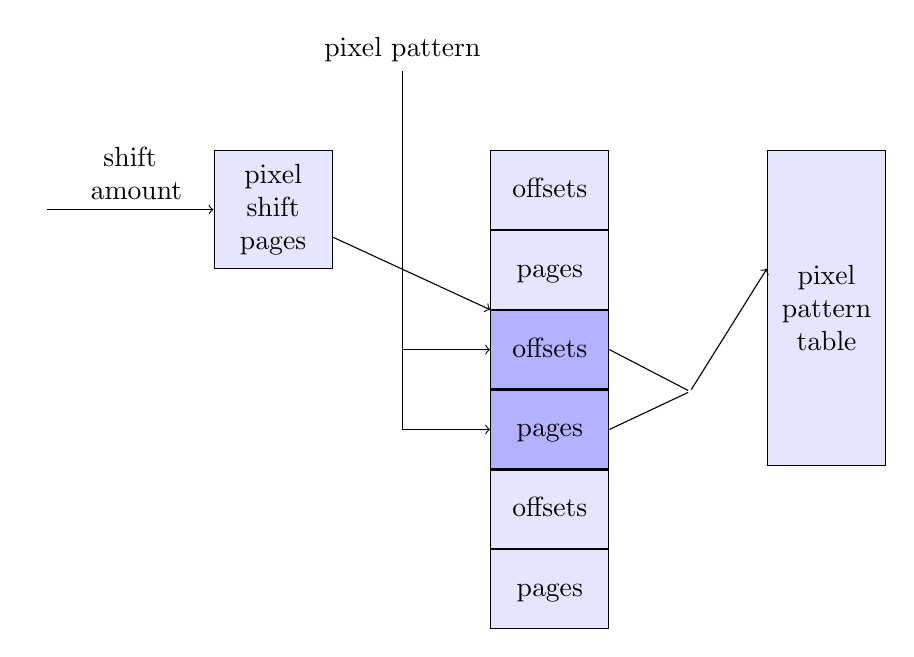
\begin{tikzpicture}
  [basicbox/.style={draw,rectangle,inner sep=0pt,minimum width=1.5cm,minimum height=1.5cm,fill=blue!10},
   pageoffsets/.style={basicbox,minimum height=1cm,text height=1.5ex,text depth=.25ex},
   multilinebox/.style={basicbox,text width=1cm,align=center}]
  \node (pixelshiftpages) at (0,0) [multilinebox] {pixel shift pages};
  \node (start) at (-3,0) {};
  \draw [->] (start) -- (pixelshiftpages) node [above,text width=1cm,align=center,midway] {shift amount};
  \node (offsets0) [pageoffsets,anchor=north,below right=0 and 2 of pixelshiftpages.north east] {offsets};
  \node (pages0) [pageoffsets,below=0 of offsets0.south] {pages};
  \node (offsets1) [pageoffsets,below=0 of pages0.south,fill=blue!30] {offsets};
  \node (pages1) [pageoffsets,below=0 of offsets1.south,fill=blue!30] {pages};
  \node (offsets2) [pageoffsets,below=0 of pages1.south] {offsets};
  \node (pages2) [pageoffsets,below=0 of offsets2.south] {pages};
  \draw [->] (pixelshiftpages) -- (offsets1.north west) {};
  \node (pixelpattern) [above left=1 and 0 of offsets0.north west] {pixel pattern};
  \draw [->] (pixelpattern.south) |- (offsets1.west) {};
  \draw [->] (pixelpattern.south) |- (pages1.west) {};
  \node (patterntable) [multilinebox,minimum height=4cm,text width=1.2cm,anchor=north west,below right=0 and 2 of offsets0.north east] {pixel pattern table};
  \node (join) [inner sep=0pt,below right=0 and 1 of offsets1.south east] {};
  \draw (offsets1.east) -- (join);
  \draw (pages1.east) -- (join);
  \draw [->] (join) -- ([yshift=5mm]patterntable.west);
\end{tikzpicture}
\vspace{1em}

The pixel pattern table is a table of every possible pattern of 7 consecutive pixels
spread out over two bytes. This table is 512 entries, each entry being two bytes.
A naive table would have redundancy. For example the pattern {\Tt{}0000100\nwendquote} starting
at column 0 is exactly the same as the pattern {\Tt{}0001000\nwendquote} starting at column 1.
This table eliminates that redundancy.

\nwenddocs{}\nwbegincode{10}\sublabel{NW1Xx3lK-1W8AJS-2}\nwmargintag{{\nwtagstyle{}\subpageref{NW1Xx3lK-1W8AJS-2}}}\moddef{tables~{\nwtagstyle{}\subpageref{NW1Xx3lK-1W8AJS-1}}}\plusendmoddef\nwstartdeflinemarkup\nwusesondefline{\\{NW1Xx3lK-1p0Y9w-1}}\nwprevnextdefs{NW1Xx3lK-1W8AJS-1}{NW1Xx3lK-1W8AJS-3}\nwenddeflinemarkup
    ORG     $A900
\nwlinkedidentc{PIXEL_PATTERN_TABLE}{NW1Xx3lK-1W8AJS-2}:
    INCLUDE "pixel_pattern_table.asm"
\nwindexdefn{\nwixident{PIXEL{\_}PATTERN{\_}TABLE}}{PIXEL:unPATTERN:unTABLE}{NW1Xx3lK-1W8AJS-2}\eatline
\nwused{\\{NW1Xx3lK-1p0Y9w-1}}\nwidentdefs{\\{{\nwixident{PIXEL{\_}PATTERN{\_}TABLE}}{PIXEL:unPATTERN:unTABLE}}}\nwendcode{}\nwbegindocs{11}\nwdocspar
Now we just need tables which index into {\Tt{}\nwlinkedidentq{PIXEL{\_}PATTERN{\_}TABLE}{NW1Xx3lK-1W8AJS-2}\nwendquote} for every
7-pixel pattern and shift value. This table works by having the page number
for the shifted pixel pattern at index {\Tt{}shift\ *\ 0x100\ +\ 0x80\ +\ pattern\nwendquote}
and the offset at index {\Tt{}shift\ *\ 0x100\ +\ pattern\nwendquote}.

\nwenddocs{}\nwbegincode{12}\sublabel{NW1Xx3lK-1W8AJS-3}\nwmargintag{{\nwtagstyle{}\subpageref{NW1Xx3lK-1W8AJS-3}}}\moddef{tables~{\nwtagstyle{}\subpageref{NW1Xx3lK-1W8AJS-1}}}\plusendmoddef\nwstartdeflinemarkup\nwusesondefline{\\{NW1Xx3lK-1p0Y9w-1}}\nwprevnextdefs{NW1Xx3lK-1W8AJS-2}{NW1Xx3lK-1W8AJS-4}\nwenddeflinemarkup
    ORG     $A200
\nwlinkedidentc{PIXEL_SHIFT_TABLE}{NW1Xx3lK-1W8AJS-3}:
    INCLUDE "pixel_shift_table.asm"
\nwindexdefn{\nwixident{PIXEL{\_}SHIFT{\_}TABLE}}{PIXEL:unSHIFT:unTABLE}{NW1Xx3lK-1W8AJS-3}\eatline
\nwused{\\{NW1Xx3lK-1p0Y9w-1}}\nwidentdefs{\\{{\nwixident{PIXEL{\_}SHIFT{\_}TABLE}}{PIXEL:unSHIFT:unTABLE}}}\nwendcode{}\nwbegindocs{13}\nwdocspar
Rather than multiplying the shift value by {\Tt{}0x100\nwendquote}, we instead define
another table which holds the page numbers for the shift tables for each
shift value.

\nwenddocs{}\nwbegincode{14}\sublabel{NW1Xx3lK-1W8AJS-4}\nwmargintag{{\nwtagstyle{}\subpageref{NW1Xx3lK-1W8AJS-4}}}\moddef{tables~{\nwtagstyle{}\subpageref{NW1Xx3lK-1W8AJS-1}}}\plusendmoddef\nwstartdeflinemarkup\nwusesondefline{\\{NW1Xx3lK-1p0Y9w-1}}\nwprevnextdefs{NW1Xx3lK-1W8AJS-3}{NW1Xx3lK-1W8AJS-5}\nwenddeflinemarkup
    ORG     $84C1
\nwlinkedidentc{PIXEL_SHIFT_PAGES}{NW1Xx3lK-1W8AJS-4}:
    HEX     A2 A3 A4 A5 A6 A7 A8
\nwindexdefn{\nwixident{PIXEL{\_}SHIFT{\_}PAGES}}{PIXEL:unSHIFT:unPAGES}{NW1Xx3lK-1W8AJS-4}\eatline
\nwused{\\{NW1Xx3lK-1p0Y9w-1}}\nwidentdefs{\\{{\nwixident{PIXEL{\_}SHIFT{\_}PAGES}}{PIXEL:unSHIFT:unPAGES}}}\nwendcode{}\nwbegindocs{15}\nwdocspar
So we can get shifted pixels by indexing into all these tables.

Now we can define a routine that will take a sprite number and a pixel shift
amount, and write the shifted pixel data into the {\Tt{}\nwlinkedidentq{BLOCK{\_}DATA}{NW1Xx3lK-10jlgu-2}\nwendquote} area. The
routine first shifts the first byte of the sprite into a two-byte area. Then
it shifts the second byte of the sprite, and combines that two-byte result
with the first. Thus, we shift two bytes of sprite data into a three-byte
result.

\begin{center}
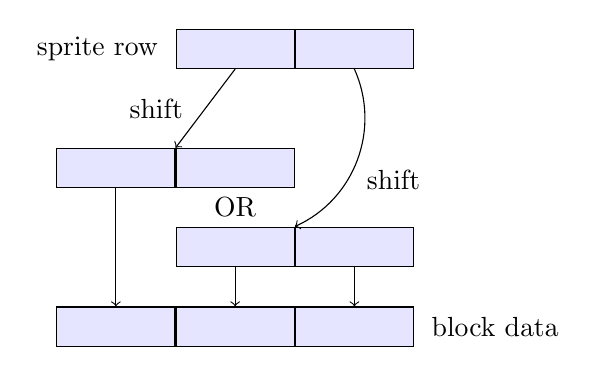
\begin{tikzpicture}
  [basicbox/.style={draw,rectangle,inner sep=0pt,minimum width=1.5cm,minimum height=0.5cm,fill=blue!10}]
  \node (spriterowbyte0) at (0,0) [basicbox] {};
  \node (spriterowbyte1) [basicbox,right=0 of spriterowbyte0.east] {};
  \node (spriterowlabel) [left=0.1 of spriterowbyte0.west] {sprite row};
  \node (shifted0byte0) [basicbox,below left=1 and 0 of spriterowbyte0.south west] {};
  \node (shifted0byte1) [basicbox,right=0 of shifted0byte0.east] {};
  \node (shifted1byte0) [basicbox,below right=2 and 0 of spriterowbyte0.south west] {};
  \node (shifted1byte1) [basicbox,right=0 of shifted1byte0.east] {};
  \node (orlabel) [below=0 of shifted0byte1] {OR};
  \draw [->] (spriterowbyte0.south) -- (shifted0byte0.north east)
    node [left,text width=1cm,align=center,midway] {shift};
  \draw [->] (spriterowbyte1.south) to [auto, bend left=45] node {shift} (shifted1byte0.north east);
  \node (result0) [basicbox,below left=0.5 and 0 of shifted1byte0.south west] {};
  \node (result1) [basicbox,right=0 of result0.east] {};
  \node (result2) [basicbox,right=0 of result1.east] {};
  \draw [->] (shifted0byte0) -- (result0) {};
  \draw [->] (shifted1byte0) -- (result1) {};
  \draw [->] (shifted1byte1) -- (result2) {};
  \node (blocklabel) [right=0.1 of result2.east] {block data};
\end{tikzpicture}
\end{center}

Rather than load addresses from the tables and store them, the routine
modifies its own instructions with those addresses.

\nwenddocs{}\nwbegincode{16}\sublabel{NW1Xx3lK-10jlgu-3}\nwmargintag{{\nwtagstyle{}\subpageref{NW1Xx3lK-10jlgu-3}}}\moddef{defines~{\nwtagstyle{}\subpageref{NW1Xx3lK-10jlgu-1}}}\plusendmoddef\nwstartdeflinemarkup\nwusesondefline{\\{NW1Xx3lK-1p0Y9w-1}}\nwprevnextdefs{NW1Xx3lK-10jlgu-2}{NW1Xx3lK-10jlgu-4}\nwenddeflinemarkup
    ORG     $1D
\nwlinkedidentc{ROW_COUNT}{NW1Xx3lK-10jlgu-3}       DS      1
\nwlinkedidentc{SPRITE_NUM}{NW1Xx3lK-10jlgu-3}      DS      1
\nwindexdefn{\nwixident{ROW{\_}COUNT}}{ROW:unCOUNT}{NW1Xx3lK-10jlgu-3}\nwindexdefn{\nwixident{SPRITE{\_}NUM}}{SPRITE:unNUM}{NW1Xx3lK-10jlgu-3}\eatline
\nwused{\\{NW1Xx3lK-1p0Y9w-1}}\nwidentdefs{\\{{\nwixident{ROW{\_}COUNT}}{ROW:unCOUNT}}\\{{\nwixident{SPRITE{\_}NUM}}{SPRITE:unNUM}}}\nwendcode{}\nwbegindocs{17}\nwdocspar
\nwenddocs{}\nwbegincode{18}\sublabel{NW1Xx3lK-8jv1b-2}\nwmargintag{{\nwtagstyle{}\subpageref{NW1Xx3lK-8jv1b-2}}}\moddef{routines~{\nwtagstyle{}\subpageref{NW1Xx3lK-8jv1b-1}}}\plusendmoddef\nwstartdeflinemarkup\nwusesondefline{\\{NW1Xx3lK-1p0Y9w-1}}\nwprevnextdefs{NW1Xx3lK-8jv1b-1}{NW1Xx3lK-8jv1b-3}\nwenddeflinemarkup
    ORG     $8438
\nwlinkedidentc{COMPUTE_SHIFTED_SPRITE}{NW1Xx3lK-8jv1b-2}:
    SUBROUTINE
    ; Enter routine with X set to pixel shift amount and
    ; \nwlinkedidentc{SPRITE_NUM}{NW1Xx3lK-10jlgu-3} containing the sprite number to read.

.offset_table       EQU $A000               ; Target addresses in read
.page_table         EQU $A080               ; instructions. The only truly
.shift_ptr_byte0    EQU $A000               ; necessary value here is the
.shift_ptr_byte1    EQU $A000               ; 0x80 in .shift_ptr_byte0.

    LDA     #$0B                            ; 11 rows
    STA     \nwlinkedidentc{ROW_COUNT}{NW1Xx3lK-10jlgu-3}
    LDA     #<\nwlinkedidentc{SPRITE_DATA}{NW1Xx3lK-1W8AJS-1}
    STA     \nwlinkedidentc{TMP_PTR}{NW1Xx3lK-10jlgu-1}
    LDA     #>\nwlinkedidentc{SPRITE_DATA}{NW1Xx3lK-1W8AJS-1}
    STA     \nwlinkedidentc{TMP_PTR}{NW1Xx3lK-10jlgu-1}+1                       ; \nwlinkedidentc{TMP_PTR}{NW1Xx3lK-10jlgu-1} = \nwlinkedidentc{SPRITE_DATA}{NW1Xx3lK-1W8AJS-1}
    LDA     \nwlinkedidentc{PIXEL_SHIFT_PAGES}{NW1Xx3lK-1W8AJS-4},X 
    STA     .rd_offset_table + 2
    STA     .rd_page_table + 2
    STA     .rd_offset_table2 + 2
    STA     .rd_page_table2 + 2             ; Fix up pages in lookup instructions
                                            ; based on shift amount (X).

    LDX     #$00                            ; X is the offset into \nwlinkedidentc{BLOCK_DATA}{NW1Xx3lK-10jlgu-2}.

.loop:                                      ; === LOOP === (over all 11 rows)
    LDY     \nwlinkedidentc{SPRITE_NUM}{NW1Xx3lK-10jlgu-3}
    LDA     (\nwlinkedidentc{TMP_PTR}{NW1Xx3lK-10jlgu-1}),Y 
    TAY                                     ; Get sprite pixel data.

.rd_offset_table:
    LDA     .offset_table,Y                 ; Load offset for shift amount.
    STA     .rd_shift_ptr_byte0 + 1
    CLC
    ADC     #$01
    STA     .rd_shift_ptr_byte1 + 1         ; Fix up instruction offsets with it.
.rd_page_table:
    LDA     .page_table,Y                   ; Load page for shift amount.
    STA     .rd_shift_ptr_byte0 + 2
    STA     .rd_shift_ptr_byte1 + 2         ; Fix up instruction page with it.

.rd_shift_ptr_byte0:
    LDA     .shift_ptr_byte0                ; Read shifted pixel data byte 0
    STA     \nwlinkedidentc{BLOCK_DATA}{NW1Xx3lK-10jlgu-2},X                    ; and store in block data byte 0.
.rd_shift_ptr_byte1:
    LDA     .shift_ptr_byte1                ; Read shifted pixel data byte 1
    STA     \nwlinkedidentc{BLOCK_DATA}{NW1Xx3lK-10jlgu-2}+1,X                  ; and store in block data byte 1.

    LDA     \nwlinkedidentc{TMP_PTR}{NW1Xx3lK-10jlgu-1}
    CLC
    ADC     #$68
    STA     \nwlinkedidentc{TMP_PTR}{NW1Xx3lK-10jlgu-1}
    LDA     \nwlinkedidentc{TMP_PTR}{NW1Xx3lK-10jlgu-1}+1
    ADC     #$00
    STA     \nwlinkedidentc{TMP_PTR}{NW1Xx3lK-10jlgu-1}+1                       ; \nwlinkedidentc{TMP_PTR}{NW1Xx3lK-10jlgu-1}++

    ; Now basically do the same thing with the second sprite byte

    LDY     \nwlinkedidentc{SPRITE_NUM}{NW1Xx3lK-10jlgu-3}
    LDA     (\nwlinkedidentc{TMP_PTR}{NW1Xx3lK-10jlgu-1}),Y 
    TAY                                     ; Get sprite pixel data.

.rd_offset_table2:
    LDA     .offset_table,Y                 ; Load offset for shift amount.
    STA     .rd_shift_ptr2_byte0 + 1
    CLC
    ADC     #$01
    STA     .rd_shift_ptr2_byte1 + 1        ; Fix up instruction offsets with it.
.rd_page_table2:
    LDA     .page_table,Y                   ; Load page for shift amount.
    STA     .rd_shift_ptr2_byte0 + 2
    STA     .rd_shift_ptr2_byte1 + 2        ; Fix up instruction page with it.

.rd_shift_ptr2_byte0:
    LDA     .shift_ptr_byte0                ; Read shifted pixel data byte 0
    ORA     \nwlinkedidentc{BLOCK_DATA}{NW1Xx3lK-10jlgu-2}+1,X                  ; OR with previous block data byte 1
    STA     \nwlinkedidentc{BLOCK_DATA}{NW1Xx3lK-10jlgu-2}+1,X                  ; and store in block data byte 1.
.rd_shift_ptr2_byte1:
    LDA     .shift_ptr_byte1                ; Read shifted pixel data byte 1
    STA     \nwlinkedidentc{BLOCK_DATA}{NW1Xx3lK-10jlgu-2}+2,X                  ; and store in block data byte 2.

    LDA     \nwlinkedidentc{TMP_PTR}{NW1Xx3lK-10jlgu-1}
    CLC
    ADC     #$68
    STA     \nwlinkedidentc{TMP_PTR}{NW1Xx3lK-10jlgu-1}
    LDA     \nwlinkedidentc{TMP_PTR}{NW1Xx3lK-10jlgu-1}+1
    ADC     #$00
    STA     \nwlinkedidentc{TMP_PTR}{NW1Xx3lK-10jlgu-1}+1                       ; \nwlinkedidentc{TMP_PTR}{NW1Xx3lK-10jlgu-1}++

    INX
    INX
    INX                                     ; X += 3
    DEC     \nwlinkedidentc{ROW_COUNT}{NW1Xx3lK-10jlgu-3}                       ; \nwlinkedidentc{ROW_COUNT}{NW1Xx3lK-10jlgu-3}--
    BNE     .loop                           ; loop while \nwlinkedidentc{ROW_COUNT}{NW1Xx3lK-10jlgu-3} > 0
    RTS
\nwindexdefn{\nwixident{COMPUTE{\_}SHIFTED{\_}SPRITE}}{COMPUTE:unSHIFTED:unSPRITE}{NW1Xx3lK-8jv1b-2}\eatline
\nwused{\\{NW1Xx3lK-1p0Y9w-1}}\nwidentdefs{\\{{\nwixident{COMPUTE{\_}SHIFTED{\_}SPRITE}}{COMPUTE:unSHIFTED:unSPRITE}}}\nwidentuses{\\{{\nwixident{BLOCK{\_}DATA}}{BLOCK:unDATA}}\\{{\nwixident{PIXEL{\_}SHIFT{\_}PAGES}}{PIXEL:unSHIFT:unPAGES}}\\{{\nwixident{ROW{\_}COUNT}}{ROW:unCOUNT}}\\{{\nwixident{SPRITE{\_}DATA}}{SPRITE:unDATA}}\\{{\nwixident{SPRITE{\_}NUM}}{SPRITE:unNUM}}\\{{\nwixident{TMP{\_}PTR}}{TMP:unPTR}}}\nwindexuse{\nwixident{BLOCK{\_}DATA}}{BLOCK:unDATA}{NW1Xx3lK-8jv1b-2}\nwindexuse{\nwixident{PIXEL{\_}SHIFT{\_}PAGES}}{PIXEL:unSHIFT:unPAGES}{NW1Xx3lK-8jv1b-2}\nwindexuse{\nwixident{ROW{\_}COUNT}}{ROW:unCOUNT}{NW1Xx3lK-8jv1b-2}\nwindexuse{\nwixident{SPRITE{\_}DATA}}{SPRITE:unDATA}{NW1Xx3lK-8jv1b-2}\nwindexuse{\nwixident{SPRITE{\_}NUM}}{SPRITE:unNUM}{NW1Xx3lK-8jv1b-2}\nwindexuse{\nwixident{TMP{\_}PTR}}{TMP:unPTR}{NW1Xx3lK-8jv1b-2}\nwendcode{}\nwbegindocs{19}\nwdocspar
\section{Memory mapped graphics}

Within a screen row, consecutive bytes map to consecutive pixels. However, rows
themselves are not consecutive in memory.

To make it easy to convert a row number from 0 to 191 to a base address, Lode Runner has
a table and a routine to use that table.

\nwenddocs{}\nwbegincode{20}\sublabel{NW1Xx3lK-1W8AJS-5}\nwmargintag{{\nwtagstyle{}\subpageref{NW1Xx3lK-1W8AJS-5}}}\moddef{tables~{\nwtagstyle{}\subpageref{NW1Xx3lK-1W8AJS-1}}}\plusendmoddef\nwstartdeflinemarkup\nwusesondefline{\\{NW1Xx3lK-1p0Y9w-1}}\nwprevnextdefs{NW1Xx3lK-1W8AJS-4}{NW1Xx3lK-1W8AJS-6}\nwenddeflinemarkup
    ORG     $1A85
\nwlinkedidentc{ROW_TO_OFFSET_LO}{NW1Xx3lK-1W8AJS-5}:
    INCLUDE "row_to_offset_lo_table.asm"
\nwlinkedidentc{ROW_TO_OFFSET_HI}{NW1Xx3lK-1W8AJS-5}:
    INCLUDE "row_to_offset_hi_table.asm"
\nwindexdefn{\nwixident{ROW{\_}TO{\_}OFFSET{\_}LO}}{ROW:unTO:unOFFSET:unLO}{NW1Xx3lK-1W8AJS-5}\nwindexdefn{\nwixident{ROW{\_}TO{\_}OFFSET{\_}HI}}{ROW:unTO:unOFFSET:unHI}{NW1Xx3lK-1W8AJS-5}\eatline
\nwused{\\{NW1Xx3lK-1p0Y9w-1}}\nwidentdefs{\\{{\nwixident{ROW{\_}TO{\_}OFFSET{\_}HI}}{ROW:unTO:unOFFSET:unHI}}\\{{\nwixident{ROW{\_}TO{\_}OFFSET{\_}LO}}{ROW:unTO:unOFFSET:unLO}}}\nwendcode{}\nwbegindocs{21}\nwdocspar
\nwenddocs{}\nwbegincode{22}\sublabel{NW1Xx3lK-10jlgu-4}\nwmargintag{{\nwtagstyle{}\subpageref{NW1Xx3lK-10jlgu-4}}}\moddef{defines~{\nwtagstyle{}\subpageref{NW1Xx3lK-10jlgu-1}}}\plusendmoddef\nwstartdeflinemarkup\nwusesondefline{\\{NW1Xx3lK-1p0Y9w-1}}\nwprevnextdefs{NW1Xx3lK-10jlgu-3}{NW1Xx3lK-10jlgu-5}\nwenddeflinemarkup
\nwlinkedidentc{ROW_ADDR}{NW1Xx3lK-10jlgu-4}        EQU     $0C     ; 2 bytes
\nwlinkedidentc{ROW_ADDR2}{NW1Xx3lK-10jlgu-4}       EQU     $0E     ; 2 bytes
\nwlinkedidentc{HGR_PAGE}{NW1Xx3lK-10jlgu-4}        EQU     $1F     ; 0x20 for HGR1, 0x40 for HGR2
\nwindexdefn{\nwixident{ROW{\_}ADDR}}{ROW:unADDR}{NW1Xx3lK-10jlgu-4}\nwindexdefn{\nwixident{ROW{\_}ADDR2}}{ROW:unADDR2}{NW1Xx3lK-10jlgu-4}\nwindexdefn{\nwixident{HGR{\_}PAGE}}{HGR:unPAGE}{NW1Xx3lK-10jlgu-4}\eatline
\nwused{\\{NW1Xx3lK-1p0Y9w-1}}\nwidentdefs{\\{{\nwixident{HGR{\_}PAGE}}{HGR:unPAGE}}\\{{\nwixident{ROW{\_}ADDR}}{ROW:unADDR}}\\{{\nwixident{ROW{\_}ADDR2}}{ROW:unADDR2}}}\nwendcode{}\nwbegindocs{23}\nwdocspar
\nwenddocs{}\nwbegincode{24}\sublabel{NW1Xx3lK-8jv1b-3}\nwmargintag{{\nwtagstyle{}\subpageref{NW1Xx3lK-8jv1b-3}}}\moddef{routines~{\nwtagstyle{}\subpageref{NW1Xx3lK-8jv1b-1}}}\plusendmoddef\nwstartdeflinemarkup\nwusesondefline{\\{NW1Xx3lK-1p0Y9w-1}}\nwprevnextdefs{NW1Xx3lK-8jv1b-2}{NW1Xx3lK-8jv1b-4}\nwenddeflinemarkup
    ORG     $7A31
\nwlinkedidentc{ROW_TO_ADDR}{NW1Xx3lK-8jv1b-3}:
    SUBROUTINE
    ; Enter routine with Y set to row. Base address
    ; (for column 0) will be placed in \nwlinkedidentc{ROW_ADDR}{NW1Xx3lK-10jlgu-4}.

    LDA     \nwlinkedidentc{ROW_TO_OFFSET_LO}{NW1Xx3lK-1W8AJS-5},Y 
    STA     \nwlinkedidentc{ROW_ADDR}{NW1Xx3lK-10jlgu-4}
    LDA     \nwlinkedidentc{ROW_TO_OFFSET_HI}{NW1Xx3lK-1W8AJS-5},Y 
    ORA     \nwlinkedidentc{HGR_PAGE}{NW1Xx3lK-10jlgu-4}
    STA     \nwlinkedidentc{ROW_ADDR}{NW1Xx3lK-10jlgu-4}+1
    RTS
\nwindexdefn{\nwixident{ROW{\_}TO{\_}ADDR}}{ROW:unTO:unADDR}{NW1Xx3lK-8jv1b-3}\eatline
\nwused{\\{NW1Xx3lK-1p0Y9w-1}}\nwidentdefs{\\{{\nwixident{ROW{\_}TO{\_}ADDR}}{ROW:unTO:unADDR}}}\nwidentuses{\\{{\nwixident{HGR{\_}PAGE}}{HGR:unPAGE}}\\{{\nwixident{ROW{\_}ADDR}}{ROW:unADDR}}\\{{\nwixident{ROW{\_}TO{\_}OFFSET{\_}HI}}{ROW:unTO:unOFFSET:unHI}}\\{{\nwixident{ROW{\_}TO{\_}OFFSET{\_}LO}}{ROW:unTO:unOFFSET:unLO}}}\nwindexuse{\nwixident{HGR{\_}PAGE}}{HGR:unPAGE}{NW1Xx3lK-8jv1b-3}\nwindexuse{\nwixident{ROW{\_}ADDR}}{ROW:unADDR}{NW1Xx3lK-8jv1b-3}\nwindexuse{\nwixident{ROW{\_}TO{\_}OFFSET{\_}HI}}{ROW:unTO:unOFFSET:unHI}{NW1Xx3lK-8jv1b-3}\nwindexuse{\nwixident{ROW{\_}TO{\_}OFFSET{\_}LO}}{ROW:unTO:unOFFSET:unLO}{NW1Xx3lK-8jv1b-3}\nwendcode{}\nwbegindocs{25}\nwdocspar
There's also a routine to load the address for both page 1 and page 2.

\nwenddocs{}\nwbegincode{26}\sublabel{NW1Xx3lK-8jv1b-4}\nwmargintag{{\nwtagstyle{}\subpageref{NW1Xx3lK-8jv1b-4}}}\moddef{routines~{\nwtagstyle{}\subpageref{NW1Xx3lK-8jv1b-1}}}\plusendmoddef\nwstartdeflinemarkup\nwusesondefline{\\{NW1Xx3lK-1p0Y9w-1}}\nwprevnextdefs{NW1Xx3lK-8jv1b-3}{NW1Xx3lK-8jv1b-5}\nwenddeflinemarkup
    ORG     $7A3E
\nwlinkedidentc{ROW_TO_ADDR_FOR_BOTH_PAGES}{NW1Xx3lK-8jv1b-4}:
    SUBROUTINE
    ; Enter routine with Y set to row. Base address
    ; (for column 0) will be placed in \nwlinkedidentc{ROW_ADDR}{NW1Xx3lK-10jlgu-4} (for page 1)
    ; and \nwlinkedidentc{ROW_ADDR2}{NW1Xx3lK-10jlgu-4} (for page 2).

    LDA     \nwlinkedidentc{ROW_TO_OFFSET_LO}{NW1Xx3lK-1W8AJS-5},Y 
    STA     \nwlinkedidentc{ROW_ADDR}{NW1Xx3lK-10jlgu-4}
    STA     \nwlinkedidentc{ROW_ADDR2}{NW1Xx3lK-10jlgu-4}
    LDA     \nwlinkedidentc{ROW_TO_OFFSET_HI}{NW1Xx3lK-1W8AJS-5},Y 
    ORA     #$20
    STA     \nwlinkedidentc{ROW_ADDR}{NW1Xx3lK-10jlgu-4}+1
    EOR     #$60
    STA     \nwlinkedidentc{ROW_ADDR2}{NW1Xx3lK-10jlgu-4}+1
    RTS
\nwindexdefn{\nwixident{ROW{\_}TO{\_}ADDR{\_}FOR{\_}BOTH{\_}PAGES}}{ROW:unTO:unADDR:unFOR:unBOTH:unPAGES}{NW1Xx3lK-8jv1b-4}\eatline
\nwused{\\{NW1Xx3lK-1p0Y9w-1}}\nwidentdefs{\\{{\nwixident{ROW{\_}TO{\_}ADDR{\_}FOR{\_}BOTH{\_}PAGES}}{ROW:unTO:unADDR:unFOR:unBOTH:unPAGES}}}\nwidentuses{\\{{\nwixident{ROW{\_}ADDR}}{ROW:unADDR}}\\{{\nwixident{ROW{\_}ADDR2}}{ROW:unADDR2}}\\{{\nwixident{ROW{\_}TO{\_}OFFSET{\_}HI}}{ROW:unTO:unOFFSET:unHI}}\\{{\nwixident{ROW{\_}TO{\_}OFFSET{\_}LO}}{ROW:unTO:unOFFSET:unLO}}}\nwindexuse{\nwixident{ROW{\_}ADDR}}{ROW:unADDR}{NW1Xx3lK-8jv1b-4}\nwindexuse{\nwixident{ROW{\_}ADDR2}}{ROW:unADDR2}{NW1Xx3lK-8jv1b-4}\nwindexuse{\nwixident{ROW{\_}TO{\_}OFFSET{\_}HI}}{ROW:unTO:unOFFSET:unHI}{NW1Xx3lK-8jv1b-4}\nwindexuse{\nwixident{ROW{\_}TO{\_}OFFSET{\_}LO}}{ROW:unTO:unOFFSET:unLO}{NW1Xx3lK-8jv1b-4}\nwendcode{}\nwbegindocs{27}\nwdocspar

Lode Runner's screens are organized into 28 sprites across by 17 sprites
down. To convert between sprite coordinates and screen coordinates, we
use tables and lookup routines. Each sprite is 10 pixels across by 11 pixels down.

\nwenddocs{}\nwbegincode{28}\sublabel{NW1Xx3lK-1W8AJS-6}\nwmargintag{{\nwtagstyle{}\subpageref{NW1Xx3lK-1W8AJS-6}}}\moddef{tables~{\nwtagstyle{}\subpageref{NW1Xx3lK-1W8AJS-1}}}\plusendmoddef\nwstartdeflinemarkup\nwusesondefline{\\{NW1Xx3lK-1p0Y9w-1}}\nwprevnextdefs{NW1Xx3lK-1W8AJS-5}{NW1Xx3lK-1W8AJS-7}\nwenddeflinemarkup
    ORG     $1C35
\nwlinkedidentc{ROW_TABLE2}{NW1Xx3lK-1W8AJS-6}:
    ; 28 rows of 5 pixels each
    HEX     00 05 0a 0f 14 19 1e 23 28 2d 32 37 3c 41 46 4b
    HEX     50 55 5a 5f 64 69 6e 73 78 7d 82 87
\nwlinkedidentc{ROW_TABLE}{NW1Xx3lK-1W8AJS-6}:
    ; 17 rows of 11 pixels each
    HEX     00 0B 16 21 2C 37 42 4D 58 63 6E 79 84 8F 9A A5
    HEX     B5
\nwlinkedidentc{COL_TABLE}{NW1Xx3lK-1W8AJS-6}:
    ; Byte number
    HEX     00 01 02 04 05 07 08 0A 0B 0C 0E 0F 11 12 14 15
    HEX     16 18 19 1B 1C 1E 1F 20 22 23 25 26
\nwlinkedidentc{COL_SHIFT_TABLE}{NW1Xx3lK-1W8AJS-6}:
    ; Right shift amount
    HEX     00 03 06 02 05 01 04 00 03 06 02 05 01 04 00 03
    HEX     06 02 05 01 04 00 03 06 02 05 01 04
\nwindexdefn{\nwixident{ROW{\_}TABLE}}{ROW:unTABLE}{NW1Xx3lK-1W8AJS-6}\nwindexdefn{\nwixident{COL{\_}TABLE}}{COL:unTABLE}{NW1Xx3lK-1W8AJS-6}\nwindexdefn{\nwixident{ROW{\_}TABLE2}}{ROW:unTABLE2}{NW1Xx3lK-1W8AJS-6}\nwindexdefn{\nwixident{COL{\_}SHIFT{\_}TABLE}}{COL:unSHIFT:unTABLE}{NW1Xx3lK-1W8AJS-6}\eatline
\nwused{\\{NW1Xx3lK-1p0Y9w-1}}\nwidentdefs{\\{{\nwixident{COL{\_}SHIFT{\_}TABLE}}{COL:unSHIFT:unTABLE}}\\{{\nwixident{COL{\_}TABLE}}{COL:unTABLE}}\\{{\nwixident{ROW{\_}TABLE}}{ROW:unTABLE}}\\{{\nwixident{ROW{\_}TABLE2}}{ROW:unTABLE2}}}\nwendcode{}\nwbegindocs{29}\nwdocspar
\nwenddocs{}\nwbegincode{30}\sublabel{NW1Xx3lK-8jv1b-5}\nwmargintag{{\nwtagstyle{}\subpageref{NW1Xx3lK-8jv1b-5}}}\moddef{routines~{\nwtagstyle{}\subpageref{NW1Xx3lK-8jv1b-1}}}\plusendmoddef\nwstartdeflinemarkup\nwusesondefline{\\{NW1Xx3lK-1p0Y9w-1}}\nwprevnextdefs{NW1Xx3lK-8jv1b-4}{NW1Xx3lK-8jv1b-6}\nwenddeflinemarkup
    ORG     $885D
\nwlinkedidentc{GET_ROWNUM_FOR}{NW1Xx3lK-8jv1b-5}:
    SUBROUTINE
    ; Enter routine with Y set to sprite row. On
    ; return,Y  will be set to screen row.
    ; We can also set X to something, and on return
    ; X is set to something based on \nwlinkedidentc{ROW_TABLE2}{NW1Xx3lK-1W8AJS-6}, but
    ; so far I'm not sure what it's used for.

    LDA     \nwlinkedidentc{ROW_TABLE}{NW1Xx3lK-1W8AJS-6},Y 
    PHA
    LDA     \nwlinkedidentc{ROW_TABLE2}{NW1Xx3lK-1W8AJS-6},X 
    TAX                         ; X = \nwlinkedidentc{ROW_TABLE2}{NW1Xx3lK-1W8AJS-6}[X]
    PLA
    TAY                         ; Y = \nwlinkedidentc{ROW_TABLE}{NW1Xx3lK-1W8AJS-6}[Y]
    RTS

\nwlinkedidentc{GET_COLNUM_FOR}{NW1Xx3lK-8jv1b-5}:
    SUBROUTINE
    ; Enter routine with X set to sprite number. On
    ; return, A will be set to screen column byte number
    ; and X will be set to an additional right shift amount.

    LDA     \nwlinkedidentc{COL_TABLE}{NW1Xx3lK-1W8AJS-6},X 
    PHA                         ; A = COL_TABLE2[X]
    LDA     \nwlinkedidentc{COL_SHIFT_TABLE}{NW1Xx3lK-1W8AJS-6},X 
    TAX                         ; X = \nwlinkedidentc{COL_SHIFT_TABLE}{NW1Xx3lK-1W8AJS-6}[X]
    PLA
    RTS
\nwindexdefn{\nwixident{GET{\_}ROWNUM{\_}FOR}}{GET:unROWNUM:unFOR}{NW1Xx3lK-8jv1b-5}\nwindexdefn{\nwixident{GET{\_}COLNUM{\_}FOR}}{GET:unCOLNUM:unFOR}{NW1Xx3lK-8jv1b-5}\eatline
\nwused{\\{NW1Xx3lK-1p0Y9w-1}}\nwidentdefs{\\{{\nwixident{GET{\_}COLNUM{\_}FOR}}{GET:unCOLNUM:unFOR}}\\{{\nwixident{GET{\_}ROWNUM{\_}FOR}}{GET:unROWNUM:unFOR}}}\nwidentuses{\\{{\nwixident{COL{\_}SHIFT{\_}TABLE}}{COL:unSHIFT:unTABLE}}\\{{\nwixident{COL{\_}TABLE}}{COL:unTABLE}}\\{{\nwixident{ROW{\_}TABLE}}{ROW:unTABLE}}\\{{\nwixident{ROW{\_}TABLE2}}{ROW:unTABLE2}}}\nwindexuse{\nwixident{COL{\_}SHIFT{\_}TABLE}}{COL:unSHIFT:unTABLE}{NW1Xx3lK-8jv1b-5}\nwindexuse{\nwixident{COL{\_}TABLE}}{COL:unTABLE}{NW1Xx3lK-8jv1b-5}\nwindexuse{\nwixident{ROW{\_}TABLE}}{ROW:unTABLE}{NW1Xx3lK-8jv1b-5}\nwindexuse{\nwixident{ROW{\_}TABLE2}}{ROW:unTABLE2}{NW1Xx3lK-8jv1b-5}\nwendcode{}\nwbegindocs{31}\nwdocspar
Now we can finally write the routines that draw a sprite on the screen.
There are two entry points, one to draw on HGR1, and one for HGR2.

\nwenddocs{}\nwbegincode{32}\sublabel{NW1Xx3lK-10jlgu-5}\nwmargintag{{\nwtagstyle{}\subpageref{NW1Xx3lK-10jlgu-5}}}\moddef{defines~{\nwtagstyle{}\subpageref{NW1Xx3lK-10jlgu-1}}}\plusendmoddef\nwstartdeflinemarkup\nwusesondefline{\\{NW1Xx3lK-1p0Y9w-1}}\nwprevnextdefs{NW1Xx3lK-10jlgu-4}{NW1Xx3lK-10jlgu-6}\nwenddeflinemarkup
    ORG     $1B
\nwlinkedidentc{ROWNUM}{NW1Xx3lK-10jlgu-5}          DS      1
\nwlinkedidentc{COLNUM}{NW1Xx3lK-10jlgu-5}          DS      1
    ORG     $50
MASK0           DS      1
MASK1           DS      1
    ORG     $71
\nwlinkedidentc{COL_SHIFT_AMT}{NW1Xx3lK-10jlgu-5}   DS      1
    ORG     $85
\nwlinkedidentc{GAME_COLNUM}{NW1Xx3lK-10jlgu-5}     DS      1
\nwlinkedidentc{GAME_ROWNUM}{NW1Xx3lK-10jlgu-5}     DS      1
\nwindexdefn{\nwixident{ROWNUM}}{ROWNUM}{NW1Xx3lK-10jlgu-5}\nwindexdefn{\nwixident{COLNUM}}{COLNUM}{NW1Xx3lK-10jlgu-5}\nwindexdefn{\nwixident{COL{\_}SHIFT{\_}AMT}}{COL:unSHIFT:unAMT}{NW1Xx3lK-10jlgu-5}\nwindexdefn{\nwixident{GAME{\_}COLNUM}}{GAME:unCOLNUM}{NW1Xx3lK-10jlgu-5}\nwindexdefn{\nwixident{GAME{\_}ROWNUM}}{GAME:unROWNUM}{NW1Xx3lK-10jlgu-5}\eatline
\nwused{\\{NW1Xx3lK-1p0Y9w-1}}\nwidentdefs{\\{{\nwixident{COL{\_}SHIFT{\_}AMT}}{COL:unSHIFT:unAMT}}\\{{\nwixident{COLNUM}}{COLNUM}}\\{{\nwixident{GAME{\_}COLNUM}}{GAME:unCOLNUM}}\\{{\nwixident{GAME{\_}ROWNUM}}{GAME:unROWNUM}}\\{{\nwixident{ROWNUM}}{ROWNUM}}}\nwendcode{}\nwbegindocs{33}\nwdocspar
\nwenddocs{}\nwbegincode{34}\sublabel{NW1Xx3lK-1W8AJS-7}\nwmargintag{{\nwtagstyle{}\subpageref{NW1Xx3lK-1W8AJS-7}}}\moddef{tables~{\nwtagstyle{}\subpageref{NW1Xx3lK-1W8AJS-1}}}\plusendmoddef\nwstartdeflinemarkup\nwusesondefline{\\{NW1Xx3lK-1p0Y9w-1}}\nwprevnextdefs{NW1Xx3lK-1W8AJS-6}{NW1Xx3lK-1W8AJS-8}\nwenddeflinemarkup
    ORG     $8328
\nwlinkedidentc{PIXEL_MASK0}{NW1Xx3lK-1W8AJS-7}:
    BYTE    %00000000
    BYTE    %00000001
    BYTE    %00000011
    BYTE    %00000111
    BYTE    %00001111
    BYTE    %00011111
    BYTE    %00111111
\nwlinkedidentc{PIXEL_MASK1}{NW1Xx3lK-1W8AJS-7}:
    BYTE    %11111000
    BYTE    %11110000
    BYTE    %11100000
    BYTE    %11000000
    BYTE    %10000000
    BYTE    %11111110
    BYTE    %11111100
\nwindexdefn{\nwixident{PIXEL{\_}MASK0}}{PIXEL:unMASK0}{NW1Xx3lK-1W8AJS-7}\nwindexdefn{\nwixident{PIXEL{\_}MASK1}}{PIXEL:unMASK1}{NW1Xx3lK-1W8AJS-7}\eatline
\nwused{\\{NW1Xx3lK-1p0Y9w-1}}\nwidentdefs{\\{{\nwixident{PIXEL{\_}MASK0}}{PIXEL:unMASK0}}\\{{\nwixident{PIXEL{\_}MASK1}}{PIXEL:unMASK1}}}\nwendcode{}\nwbegindocs{35}\nwdocspar
\nwenddocs{}\nwbegincode{36}\sublabel{NW1Xx3lK-8jv1b-6}\nwmargintag{{\nwtagstyle{}\subpageref{NW1Xx3lK-8jv1b-6}}}\moddef{routines~{\nwtagstyle{}\subpageref{NW1Xx3lK-8jv1b-1}}}\plusendmoddef\nwstartdeflinemarkup\nwusesondefline{\\{NW1Xx3lK-1p0Y9w-1}}\nwprevnextdefs{NW1Xx3lK-8jv1b-5}{NW1Xx3lK-8jv1b-7}\nwenddeflinemarkup
    ORG     $82AA
\nwlinkedidentc{DRAW_SPRITE_PAGE1}{NW1Xx3lK-8jv1b-6}:
    SUBROUTINE
    ; Enter routine with A set to sprite number to draw,
    ; \nwlinkedidentc{GAME_ROWNUM}{NW1Xx3lK-10jlgu-5} set to the row to draw it at, and \nwlinkedidentc{GAME_COLNUM}{NW1Xx3lK-10jlgu-5}
    ; set to the column to draw it at.

    STA     \nwlinkedidentc{SPRITE_NUM}{NW1Xx3lK-10jlgu-3}
    LDA     #$20                ; Page number for HGR1
    BNE     DRAW_SPRITE         ; Actually unconditional jump

\nwlinkedidentc{DRAW_SPRITE_PAGE2}{NW1Xx3lK-8jv1b-6}:
    SUBROUTINE
    ; Enter routine with A set to sprite number to draw,
    ; \nwlinkedidentc{GAME_ROWNUM}{NW1Xx3lK-10jlgu-5} set to the row to draw it at, and \nwlinkedidentc{GAME_COLNUM}{NW1Xx3lK-10jlgu-5}
    ; set to the column to draw it at.

    STA     \nwlinkedidentc{SPRITE_NUM}{NW1Xx3lK-10jlgu-3}
    LDA     #$40                ; Page number for HGR2
    ; fallthrough

DRAW_SPRITE:
    STA     \nwlinkedidentc{HGR_PAGE}{NW1Xx3lK-10jlgu-4}
    LDY     \nwlinkedidentc{GAME_ROWNUM}{NW1Xx3lK-10jlgu-5}
    JSR     \nwlinkedidentc{GET_ROWNUM_FOR}{NW1Xx3lK-8jv1b-5}
    STY     \nwlinkedidentc{ROWNUM}{NW1Xx3lK-10jlgu-5}              ; \nwlinkedidentc{ROWNUM}{NW1Xx3lK-10jlgu-5} = \nwlinkedidentc{ROW_TABLE}{NW1Xx3lK-1W8AJS-6}[\nwlinkedidentc{GAME_ROWNUM}{NW1Xx3lK-10jlgu-5}]

    LDX     \nwlinkedidentc{GAME_COLNUM}{NW1Xx3lK-10jlgu-5}
    JSR     \nwlinkedidentc{GET_COLNUM_FOR}{NW1Xx3lK-8jv1b-5}
    STA     \nwlinkedidentc{COLNUM}{NW1Xx3lK-10jlgu-5}              ; \nwlinkedidentc{COLNUM}{NW1Xx3lK-10jlgu-5} = \nwlinkedidentc{COL_TABLE}{NW1Xx3lK-1W8AJS-6}[\nwlinkedidentc{GAME_COLNUM}{NW1Xx3lK-10jlgu-5}]
    STX     \nwlinkedidentc{COL_SHIFT_AMT}{NW1Xx3lK-10jlgu-5}       ; \nwlinkedidentc{COL_SHIFT_AMT}{NW1Xx3lK-10jlgu-5} = \nwlinkedidentc{COL_SHIFT_TABLE}{NW1Xx3lK-1W8AJS-6}[\nwlinkedidentc{GAME_COLNUM}{NW1Xx3lK-10jlgu-5}]

    LDA     \nwlinkedidentc{PIXEL_MASK0}{NW1Xx3lK-1W8AJS-7},X 
    STA     MASK0               ; MASK0 = \nwlinkedidentc{PIXEL_MASK0}{NW1Xx3lK-1W8AJS-7}[\nwlinkedidentc{COL_SHIFT_AMT}{NW1Xx3lK-10jlgu-5}]
    LDA     \nwlinkedidentc{PIXEL_MASK1}{NW1Xx3lK-1W8AJS-7},X 
    STA     MASK1               ; MASK1 = \nwlinkedidentc{PIXEL_MASK1}{NW1Xx3lK-1W8AJS-7}[\nwlinkedidentc{COL_SHIFT_AMT}{NW1Xx3lK-10jlgu-5}]

    JSR     \nwlinkedidentc{COMPUTE_SHIFTED_SPRITE}{NW1Xx3lK-8jv1b-2}

    LDA     #$0B
    STA     \nwlinkedidentc{ROW_COUNT}{NW1Xx3lK-10jlgu-3}
    LDX     #$00
    LDA     \nwlinkedidentc{COL_SHIFT_AMT}{NW1Xx3lK-10jlgu-5}
    CMP     #$05
    BCS     .need_3_bytes       ; If \nwlinkedidentc{COL_SHIFT_AMT}{NW1Xx3lK-10jlgu-5} >= 5, we need to alter three screen bytes,
                                ; otherwise just two bytes.

.loop1:
    LDY     \nwlinkedidentc{ROWNUM}{NW1Xx3lK-10jlgu-5}
    JSR     \nwlinkedidentc{ROW_TO_ADDR}{NW1Xx3lK-8jv1b-3}
    LDY     \nwlinkedidentc{COLNUM}{NW1Xx3lK-10jlgu-5}
    LDA     (\nwlinkedidentc{ROW_ADDR}{NW1Xx3lK-10jlgu-4}),Y 
    AND     MASK0
    ORA     \nwlinkedidentc{BLOCK_DATA}{NW1Xx3lK-10jlgu-2},X 
    STA     (\nwlinkedidentc{ROW_ADDR}{NW1Xx3lK-10jlgu-4}),Y        ; screen[\nwlinkedidentc{COLNUM}{NW1Xx3lK-10jlgu-5}] = screen[\nwlinkedidentc{COLNUM}{NW1Xx3lK-10jlgu-5}] & MASK0 | \nwlinkedidentc{BLOCK_DATA}{NW1Xx3lK-10jlgu-2}[i]

    INX                         ; X++
    INY                         ; Y++
    LDA     (\nwlinkedidentc{ROW_ADDR}{NW1Xx3lK-10jlgu-4}),Y 
    AND     MASK1
    ORA     \nwlinkedidentc{BLOCK_DATA}{NW1Xx3lK-10jlgu-2},X 
    STA     (\nwlinkedidentc{ROW_ADDR}{NW1Xx3lK-10jlgu-4}),Y        ; screen[\nwlinkedidentc{COLNUM}{NW1Xx3lK-10jlgu-5}+1] = screen[\nwlinkedidentc{COLNUM}{NW1Xx3lK-10jlgu-5}+1] & MASK1 | \nwlinkedidentc{BLOCK_DATA}{NW1Xx3lK-10jlgu-2}[i+1]

    INX
    INX                         ; X += 2
    INC     \nwlinkedidentc{ROWNUM}{NW1Xx3lK-10jlgu-5}              ; \nwlinkedidentc{ROWNUM}{NW1Xx3lK-10jlgu-5}++
    DEC     \nwlinkedidentc{ROW_COUNT}{NW1Xx3lK-10jlgu-3}           ; \nwlinkedidentc{ROW_COUNT}{NW1Xx3lK-10jlgu-3}--
    BNE     .loop1              ; loop while \nwlinkedidentc{ROW_COUNT}{NW1Xx3lK-10jlgu-3} > 0
    RTS

.need_3_bytes
    LDY     \nwlinkedidentc{ROWNUM}{NW1Xx3lK-10jlgu-5}
    JSR     \nwlinkedidentc{ROW_TO_ADDR}{NW1Xx3lK-8jv1b-3}
    LDY     \nwlinkedidentc{COLNUM}{NW1Xx3lK-10jlgu-5}
    LDA     (\nwlinkedidentc{ROW_ADDR}{NW1Xx3lK-10jlgu-4}),Y 
    AND     MASK0
    ORA     \nwlinkedidentc{BLOCK_DATA}{NW1Xx3lK-10jlgu-2},X 
    STA     (\nwlinkedidentc{ROW_ADDR}{NW1Xx3lK-10jlgu-4}),Y        ; screen[\nwlinkedidentc{COLNUM}{NW1Xx3lK-10jlgu-5}] = screen[\nwlinkedidentc{COLNUM}{NW1Xx3lK-10jlgu-5}] & MASK0 | \nwlinkedidentc{BLOCK_DATA}{NW1Xx3lK-10jlgu-2}[i]

    INX                         ; X++
    INY                         ; Y++
    LDA     \nwlinkedidentc{BLOCK_DATA}{NW1Xx3lK-10jlgu-2},X 
    STA     (\nwlinkedidentc{ROW_ADDR}{NW1Xx3lK-10jlgu-4}),Y        ; screen[\nwlinkedidentc{COLNUM}{NW1Xx3lK-10jlgu-5}+1] = \nwlinkedidentc{BLOCK_DATA}{NW1Xx3lK-10jlgu-2}[i+1]

    INX                         ; X++
    INY                         ; Y++
    LDA     (\nwlinkedidentc{ROW_ADDR}{NW1Xx3lK-10jlgu-4}),Y 
    AND     MASK1
    ORA     \nwlinkedidentc{BLOCK_DATA}{NW1Xx3lK-10jlgu-2},X 
    STA     (\nwlinkedidentc{ROW_ADDR}{NW1Xx3lK-10jlgu-4}),Y        ; screen[\nwlinkedidentc{COLNUM}{NW1Xx3lK-10jlgu-5}+2] = screen[\nwlinkedidentc{COLNUM}{NW1Xx3lK-10jlgu-5}+2] & MASK1 | \nwlinkedidentc{BLOCK_DATA}{NW1Xx3lK-10jlgu-2}[i+2]

    INX                         ; X++
    INC     \nwlinkedidentc{ROWNUM}{NW1Xx3lK-10jlgu-5}              ; \nwlinkedidentc{ROWNUM}{NW1Xx3lK-10jlgu-5}++
    DEC     \nwlinkedidentc{ROW_COUNT}{NW1Xx3lK-10jlgu-3}           ; \nwlinkedidentc{ROW_COUNT}{NW1Xx3lK-10jlgu-3}--
    BNE     .need_3_bytes       ; loop while \nwlinkedidentc{ROW_COUNT}{NW1Xx3lK-10jlgu-3} > 0
    RTS
\nwindexdefn{\nwixident{DRAW{\_}SPRITE{\_}PAGE1}}{DRAW:unSPRITE:unPAGE1}{NW1Xx3lK-8jv1b-6}\nwindexdefn{\nwixident{DRAW{\_}SPRITE{\_}PAGE2}}{DRAW:unSPRITE:unPAGE2}{NW1Xx3lK-8jv1b-6}\eatline
\nwused{\\{NW1Xx3lK-1p0Y9w-1}}\nwidentdefs{\\{{\nwixident{DRAW{\_}SPRITE{\_}PAGE1}}{DRAW:unSPRITE:unPAGE1}}\\{{\nwixident{DRAW{\_}SPRITE{\_}PAGE2}}{DRAW:unSPRITE:unPAGE2}}}\nwidentuses{\\{{\nwixident{BLOCK{\_}DATA}}{BLOCK:unDATA}}\\{{\nwixident{COL{\_}SHIFT{\_}AMT}}{COL:unSHIFT:unAMT}}\\{{\nwixident{COL{\_}SHIFT{\_}TABLE}}{COL:unSHIFT:unTABLE}}\\{{\nwixident{COL{\_}TABLE}}{COL:unTABLE}}\\{{\nwixident{COLNUM}}{COLNUM}}\\{{\nwixident{COMPUTE{\_}SHIFTED{\_}SPRITE}}{COMPUTE:unSHIFTED:unSPRITE}}\\{{\nwixident{GAME{\_}COLNUM}}{GAME:unCOLNUM}}\\{{\nwixident{GAME{\_}ROWNUM}}{GAME:unROWNUM}}\\{{\nwixident{GET{\_}COLNUM{\_}FOR}}{GET:unCOLNUM:unFOR}}\\{{\nwixident{GET{\_}ROWNUM{\_}FOR}}{GET:unROWNUM:unFOR}}\\{{\nwixident{HGR{\_}PAGE}}{HGR:unPAGE}}\\{{\nwixident{PIXEL{\_}MASK0}}{PIXEL:unMASK0}}\\{{\nwixident{PIXEL{\_}MASK1}}{PIXEL:unMASK1}}\\{{\nwixident{ROW{\_}ADDR}}{ROW:unADDR}}\\{{\nwixident{ROW{\_}COUNT}}{ROW:unCOUNT}}\\{{\nwixident{ROW{\_}TABLE}}{ROW:unTABLE}}\\{{\nwixident{ROW{\_}TO{\_}ADDR}}{ROW:unTO:unADDR}}\\{{\nwixident{ROWNUM}}{ROWNUM}}\\{{\nwixident{SPRITE{\_}NUM}}{SPRITE:unNUM}}}\nwindexuse{\nwixident{BLOCK{\_}DATA}}{BLOCK:unDATA}{NW1Xx3lK-8jv1b-6}\nwindexuse{\nwixident{COL{\_}SHIFT{\_}AMT}}{COL:unSHIFT:unAMT}{NW1Xx3lK-8jv1b-6}\nwindexuse{\nwixident{COL{\_}SHIFT{\_}TABLE}}{COL:unSHIFT:unTABLE}{NW1Xx3lK-8jv1b-6}\nwindexuse{\nwixident{COL{\_}TABLE}}{COL:unTABLE}{NW1Xx3lK-8jv1b-6}\nwindexuse{\nwixident{COLNUM}}{COLNUM}{NW1Xx3lK-8jv1b-6}\nwindexuse{\nwixident{COMPUTE{\_}SHIFTED{\_}SPRITE}}{COMPUTE:unSHIFTED:unSPRITE}{NW1Xx3lK-8jv1b-6}\nwindexuse{\nwixident{GAME{\_}COLNUM}}{GAME:unCOLNUM}{NW1Xx3lK-8jv1b-6}\nwindexuse{\nwixident{GAME{\_}ROWNUM}}{GAME:unROWNUM}{NW1Xx3lK-8jv1b-6}\nwindexuse{\nwixident{GET{\_}COLNUM{\_}FOR}}{GET:unCOLNUM:unFOR}{NW1Xx3lK-8jv1b-6}\nwindexuse{\nwixident{GET{\_}ROWNUM{\_}FOR}}{GET:unROWNUM:unFOR}{NW1Xx3lK-8jv1b-6}\nwindexuse{\nwixident{HGR{\_}PAGE}}{HGR:unPAGE}{NW1Xx3lK-8jv1b-6}\nwindexuse{\nwixident{PIXEL{\_}MASK0}}{PIXEL:unMASK0}{NW1Xx3lK-8jv1b-6}\nwindexuse{\nwixident{PIXEL{\_}MASK1}}{PIXEL:unMASK1}{NW1Xx3lK-8jv1b-6}\nwindexuse{\nwixident{ROW{\_}ADDR}}{ROW:unADDR}{NW1Xx3lK-8jv1b-6}\nwindexuse{\nwixident{ROW{\_}COUNT}}{ROW:unCOUNT}{NW1Xx3lK-8jv1b-6}\nwindexuse{\nwixident{ROW{\_}TABLE}}{ROW:unTABLE}{NW1Xx3lK-8jv1b-6}\nwindexuse{\nwixident{ROW{\_}TO{\_}ADDR}}{ROW:unTO:unADDR}{NW1Xx3lK-8jv1b-6}\nwindexuse{\nwixident{ROWNUM}}{ROWNUM}{NW1Xx3lK-8jv1b-6}\nwindexuse{\nwixident{SPRITE{\_}NUM}}{SPRITE:unNUM}{NW1Xx3lK-8jv1b-6}\nwendcode{}\nwbegindocs{37}\nwdocspar
\section{Printing strings}

Now that we can put sprites onto the screen at any game coordinate, we can
also have some routines that print strings. We saw above that we have
letter and number sprites, plus some punctuation. Letters and punctuation
are always blue, while numbers are always orange.

There is a basic routine to put a character at the current {\Tt{}\nwlinkedidentq{GAME{\_}COLNUM}{NW1Xx3lK-10jlgu-5}\nwendquote}
and {\Tt{}\nwlinkedidentq{GAME{\_}ROWNUM}{NW1Xx3lK-10jlgu-5}\nwendquote}, incrementing this "cursor", and putting it at the beginning
of the next line if we "print" a newline character.

We first define a routine to convert the ASCII code of a character to
its sprite number. Lode Runner sets the high bit of the code to
make it be treated as ASCII.

\nwenddocs{}\nwbegincode{38}\sublabel{NW1Xx3lK-8jv1b-7}\nwmargintag{{\nwtagstyle{}\subpageref{NW1Xx3lK-8jv1b-7}}}\moddef{routines~{\nwtagstyle{}\subpageref{NW1Xx3lK-8jv1b-1}}}\plusendmoddef\nwstartdeflinemarkup\nwusesondefline{\\{NW1Xx3lK-1p0Y9w-1}}\nwprevnextdefs{NW1Xx3lK-8jv1b-6}{NW1Xx3lK-8jv1b-8}\nwenddeflinemarkup
    ORG     $7b2a
\nwlinkedidentc{CHAR_TO_SPRITE_NUM}{NW1Xx3lK-8jv1b-7}:
    SUBROUTINE
    ; Enter routine with A set to the ASCII code of the
    ; character to convert to sprite number, with the high bit set.
    ; The sprite number is returned in A.

    CMP     #$C1                    ; 'A' -> sprite 69
    BCC     .not_letter
    CMP     #$DB                    ; 'Z' -> sprite 94
    BCC     .letter

.not_letter:
    ; On return, we will subtract 0x7C from X to
    ; get the actual sprite. This is to make A-Z
    ; easier to handle.
    LDX     #$7C
    CMP     #$A0                    ; ' ' -> sprite 0
    BEQ     .end
    LDX     #$DB
    CMP     #$BE                    ; '>' -> sprite 95
    BEQ     .end
    INX
    CMP     #$AE                    ; '.' -> sprite 96
    BEQ     .end
    INX
    CMP     #$A8                    ; '(' -> sprite 97
    BEQ     .end
    INX
    CMP     #$A9                    ; ')' -> sprite 98
    BEQ     .end
    INX
    CMP     #$AF                    ; '/' -> sprite 99
    BEQ     .end
    INX
    CMP     #$AD                    ; '-' -> sprite 100
    BEQ     .end
    INX
    CMP     #$BC                    ; '<' -> sprite 101
    BEQ     .end
    LDA     #$10                    ; sprite 16: just one of the man sprites
    RTS

.end:
    TXA

.letter:
    SEC
    SBC     #$7C                    
    RTS

\nwindexdefn{\nwixident{CHAR{\_}TO{\_}SPRITE{\_}NUM}}{CHAR:unTO:unSPRITE:unNUM}{NW1Xx3lK-8jv1b-7}\eatline
\nwused{\\{NW1Xx3lK-1p0Y9w-1}}\nwidentdefs{\\{{\nwixident{CHAR{\_}TO{\_}SPRITE{\_}NUM}}{CHAR:unTO:unSPRITE:unNUM}}}\nwendcode{}\nwbegindocs{39}\nwdocspar
Now we can define the routine to put a character on the screen at the
current position.

\nwenddocs{}\nwbegincode{40}\sublabel{NW1Xx3lK-10jlgu-6}\nwmargintag{{\nwtagstyle{}\subpageref{NW1Xx3lK-10jlgu-6}}}\moddef{defines~{\nwtagstyle{}\subpageref{NW1Xx3lK-10jlgu-1}}}\plusendmoddef\nwstartdeflinemarkup\nwusesondefline{\\{NW1Xx3lK-1p0Y9w-1}}\nwprevnextdefs{NW1Xx3lK-10jlgu-5}{NW1Xx3lK-10jlgu-7}\nwenddeflinemarkup
\nwlinkedidentc{DRAW_PAGE}{NW1Xx3lK-10jlgu-6}   EQU     $87     ; 0x20 for page 1, 0x40 for page 2
\nwindexdefn{\nwixident{DRAW{\_}PAGE}}{DRAW:unPAGE}{NW1Xx3lK-10jlgu-6}\eatline
\nwused{\\{NW1Xx3lK-1p0Y9w-1}}\nwidentdefs{\\{{\nwixident{DRAW{\_}PAGE}}{DRAW:unPAGE}}}\nwendcode{}\nwbegindocs{41}\nwdocspar
\nwenddocs{}\nwbegincode{42}\sublabel{NW1Xx3lK-8jv1b-8}\nwmargintag{{\nwtagstyle{}\subpageref{NW1Xx3lK-8jv1b-8}}}\moddef{routines~{\nwtagstyle{}\subpageref{NW1Xx3lK-8jv1b-1}}}\plusendmoddef\nwstartdeflinemarkup\nwusesondefline{\\{NW1Xx3lK-1p0Y9w-1}}\nwprevnextdefs{NW1Xx3lK-8jv1b-7}{NW1Xx3lK-8jv1b-9}\nwenddeflinemarkup
    ORG     $7b64
\nwlinkedidentc{PUT_CHAR}{NW1Xx3lK-8jv1b-8}:
    SUBROUTINE
    ; Enter routine with A set to the ASCII code of the
    ; character to put on the screen, with the high bit set.

    CMP     #$8D
    BEQ     \nwlinkedidentc{NEWLINE}{NW1Xx3lK-8jv1b-8}                 ; If newline, do \nwlinkedidentc{NEWLINE}{NW1Xx3lK-8jv1b-8} instead.
    JSR     \nwlinkedidentc{CHAR_TO_SPRITE_NUM}{NW1Xx3lK-8jv1b-7}
    LDX     \nwlinkedidentc{DRAW_PAGE}{NW1Xx3lK-10jlgu-6}
    CPX     #$40
    BEQ     .draw_to_page2

    JSR     \nwlinkedidentc{DRAW_SPRITE_PAGE1}{NW1Xx3lK-8jv1b-6}
    INC     \nwlinkedidentc{GAME_COLNUM}{NW1Xx3lK-10jlgu-5}
    RTS

.draw_to_page2
    JSR     \nwlinkedidentc{DRAW_SPRITE_PAGE2}{NW1Xx3lK-8jv1b-6}
    INC     \nwlinkedidentc{GAME_COLNUM}{NW1Xx3lK-10jlgu-5}
    RTS

\nwlinkedidentc{NEWLINE}{NW1Xx3lK-8jv1b-8}:
    SUBROUTINE
    INC     \nwlinkedidentc{GAME_ROWNUM}{NW1Xx3lK-10jlgu-5}
    LDA     #$00
    STA     \nwlinkedidentc{GAME_COLNUM}{NW1Xx3lK-10jlgu-5}
    RTS
\nwindexdefn{\nwixident{PUT{\_}CHAR}}{PUT:unCHAR}{NW1Xx3lK-8jv1b-8}\nwindexdefn{\nwixident{NEWLINE}}{NEWLINE}{NW1Xx3lK-8jv1b-8}\eatline
\nwused{\\{NW1Xx3lK-1p0Y9w-1}}\nwidentdefs{\\{{\nwixident{NEWLINE}}{NEWLINE}}\\{{\nwixident{PUT{\_}CHAR}}{PUT:unCHAR}}}\nwidentuses{\\{{\nwixident{CHAR{\_}TO{\_}SPRITE{\_}NUM}}{CHAR:unTO:unSPRITE:unNUM}}\\{{\nwixident{DRAW{\_}PAGE}}{DRAW:unPAGE}}\\{{\nwixident{DRAW{\_}SPRITE{\_}PAGE1}}{DRAW:unSPRITE:unPAGE1}}\\{{\nwixident{DRAW{\_}SPRITE{\_}PAGE2}}{DRAW:unSPRITE:unPAGE2}}\\{{\nwixident{GAME{\_}COLNUM}}{GAME:unCOLNUM}}\\{{\nwixident{GAME{\_}ROWNUM}}{GAME:unROWNUM}}}\nwindexuse{\nwixident{CHAR{\_}TO{\_}SPRITE{\_}NUM}}{CHAR:unTO:unSPRITE:unNUM}{NW1Xx3lK-8jv1b-8}\nwindexuse{\nwixident{DRAW{\_}PAGE}}{DRAW:unPAGE}{NW1Xx3lK-8jv1b-8}\nwindexuse{\nwixident{DRAW{\_}SPRITE{\_}PAGE1}}{DRAW:unSPRITE:unPAGE1}{NW1Xx3lK-8jv1b-8}\nwindexuse{\nwixident{DRAW{\_}SPRITE{\_}PAGE2}}{DRAW:unSPRITE:unPAGE2}{NW1Xx3lK-8jv1b-8}\nwindexuse{\nwixident{GAME{\_}COLNUM}}{GAME:unCOLNUM}{NW1Xx3lK-8jv1b-8}\nwindexuse{\nwixident{GAME{\_}ROWNUM}}{GAME:unROWNUM}{NW1Xx3lK-8jv1b-8}\nwendcode{}\nwbegindocs{43}\nwdocspar
The {\Tt{}\nwlinkedidentq{PUT{\_}STRING}{NW1Xx3lK-8jv1b-9}\nwendquote} routine uses {\Tt{}\nwlinkedidentq{PUT{\_}CHAR}{NW1Xx3lK-8jv1b-8}\nwendquote} to put a string on the screen. Rather than take
an address pointing to a string, instead it uses the return address as the source for data.
It then has to fix up the actual return address at the end to be just after the zero-terminating
byte of the string.

\nwenddocs{}\nwbegincode{44}\sublabel{NW1Xx3lK-10jlgu-7}\nwmargintag{{\nwtagstyle{}\subpageref{NW1Xx3lK-10jlgu-7}}}\moddef{defines~{\nwtagstyle{}\subpageref{NW1Xx3lK-10jlgu-1}}}\plusendmoddef\nwstartdeflinemarkup\nwusesondefline{\\{NW1Xx3lK-1p0Y9w-1}}\nwprevnextdefs{NW1Xx3lK-10jlgu-6}{NW1Xx3lK-10jlgu-8}\nwenddeflinemarkup
    ORG     $10
\nwlinkedidentc{SAVED_RET_ADDR}{NW1Xx3lK-10jlgu-7}      DS.W    1
\nwindexdefn{\nwixident{SAVED{\_}RET{\_}ADDR}}{SAVED:unRET:unADDR}{NW1Xx3lK-10jlgu-7}\eatline
\nwused{\\{NW1Xx3lK-1p0Y9w-1}}\nwidentdefs{\\{{\nwixident{SAVED{\_}RET{\_}ADDR}}{SAVED:unRET:unADDR}}}\nwendcode{}\nwbegindocs{45}\nwdocspar
\nwenddocs{}\nwbegincode{46}\sublabel{NW1Xx3lK-8jv1b-9}\nwmargintag{{\nwtagstyle{}\subpageref{NW1Xx3lK-8jv1b-9}}}\moddef{routines~{\nwtagstyle{}\subpageref{NW1Xx3lK-8jv1b-1}}}\plusendmoddef\nwstartdeflinemarkup\nwusesondefline{\\{NW1Xx3lK-1p0Y9w-1}}\nwprevnextdefs{NW1Xx3lK-8jv1b-8}{NW1Xx3lK-8jv1b-A}\nwenddeflinemarkup
    ORG     $86E0
\nwlinkedidentc{PUT_STRING}{NW1Xx3lK-8jv1b-9}:
    SUBROUTINE

    PLA
    STA     \nwlinkedidentc{SAVED_RET_ADDR}{NW1Xx3lK-10jlgu-7}
    PLA
    STA     \nwlinkedidentc{SAVED_RET_ADDR}{NW1Xx3lK-10jlgu-7}+1
    BNE     .next

.loop:
    LDY     #$00
    LDA     (\nwlinkedidentc{SAVED_RET_ADDR}{NW1Xx3lK-10jlgu-7}),Y
    BEQ     .end
    JSR     \nwlinkedidentc{PUT_CHAR}{NW1Xx3lK-8jv1b-8}

.next:
    INC     \nwlinkedidentc{SAVED_RET_ADDR}{NW1Xx3lK-10jlgu-7}
    BNE     .loop
    INC     \nwlinkedidentc{SAVED_RET_ADDR}{NW1Xx3lK-10jlgu-7}+1
    BNE     .loop

.end:
    LDA     \nwlinkedidentc{SAVED_RET_ADDR}{NW1Xx3lK-10jlgu-7}+1
    PHA
    LDA     \nwlinkedidentc{SAVED_RET_ADDR}{NW1Xx3lK-10jlgu-7}
    PHA
    RTS
\nwindexdefn{\nwixident{PUT{\_}STRING}}{PUT:unSTRING}{NW1Xx3lK-8jv1b-9}\eatline
\nwused{\\{NW1Xx3lK-1p0Y9w-1}}\nwidentdefs{\\{{\nwixident{PUT{\_}STRING}}{PUT:unSTRING}}}\nwidentuses{\\{{\nwixident{PUT{\_}CHAR}}{PUT:unCHAR}}\\{{\nwixident{SAVED{\_}RET{\_}ADDR}}{SAVED:unRET:unADDR}}}\nwindexuse{\nwixident{PUT{\_}CHAR}}{PUT:unCHAR}{NW1Xx3lK-8jv1b-9}\nwindexuse{\nwixident{SAVED{\_}RET{\_}ADDR}}{SAVED:unRET:unADDR}{NW1Xx3lK-8jv1b-9}\nwendcode{}\nwbegindocs{47}\nwdocspar
Like {\Tt{}\nwlinkedidentq{PUT{\_}CHAR}{NW1Xx3lK-8jv1b-8}\nwendquote}, we also have {\Tt{}\nwlinkedidentq{PUT{\_}DIGIT}{NW1Xx3lK-8jv1b-A}\nwendquote} which draws the sprite corresponding
to digits 0 to 9 at the current position, incrementing the cursor.

\nwenddocs{}\nwbegincode{48}\sublabel{NW1Xx3lK-8jv1b-A}\nwmargintag{{\nwtagstyle{}\subpageref{NW1Xx3lK-8jv1b-A}}}\moddef{routines~{\nwtagstyle{}\subpageref{NW1Xx3lK-8jv1b-1}}}\plusendmoddef\nwstartdeflinemarkup\nwusesondefline{\\{NW1Xx3lK-1p0Y9w-1}}\nwprevnextdefs{NW1Xx3lK-8jv1b-9}{NW1Xx3lK-8jv1b-B}\nwenddeflinemarkup
    ORG     $7B15
\nwlinkedidentc{PUT_DIGIT}{NW1Xx3lK-8jv1b-A}:
    SUBROUTINE
    ; Enter routine with A set to the digit to put on the screen.

    CLC
    ADC     #$3B                    ; '0' -> sprite 59, '9' -> sprite 68.
    LDX     \nwlinkedidentc{DRAW_PAGE}{NW1Xx3lK-10jlgu-6}
    CPX     #$40
    BEQ     .draw_to_page2
    JSR     \nwlinkedidentc{DRAW_SPRITE_PAGE1}{NW1Xx3lK-8jv1b-6}
    INC     \nwlinkedidentc{GAME_COLNUM}{NW1Xx3lK-10jlgu-5}
    RTS

.draw_to_page2:
    JSR     \nwlinkedidentc{DRAW_SPRITE_PAGE2}{NW1Xx3lK-8jv1b-6}
    INC     \nwlinkedidentc{GAME_COLNUM}{NW1Xx3lK-10jlgu-5}
    RTS
\nwindexdefn{\nwixident{PUT{\_}DIGIT}}{PUT:unDIGIT}{NW1Xx3lK-8jv1b-A}\eatline
\nwused{\\{NW1Xx3lK-1p0Y9w-1}}\nwidentdefs{\\{{\nwixident{PUT{\_}DIGIT}}{PUT:unDIGIT}}}\nwidentuses{\\{{\nwixident{DRAW{\_}PAGE}}{DRAW:unPAGE}}\\{{\nwixident{DRAW{\_}SPRITE{\_}PAGE1}}{DRAW:unSPRITE:unPAGE1}}\\{{\nwixident{DRAW{\_}SPRITE{\_}PAGE2}}{DRAW:unSPRITE:unPAGE2}}\\{{\nwixident{GAME{\_}COLNUM}}{GAME:unCOLNUM}}}\nwindexuse{\nwixident{DRAW{\_}PAGE}}{DRAW:unPAGE}{NW1Xx3lK-8jv1b-A}\nwindexuse{\nwixident{DRAW{\_}SPRITE{\_}PAGE1}}{DRAW:unSPRITE:unPAGE1}{NW1Xx3lK-8jv1b-A}\nwindexuse{\nwixident{DRAW{\_}SPRITE{\_}PAGE2}}{DRAW:unSPRITE:unPAGE2}{NW1Xx3lK-8jv1b-A}\nwindexuse{\nwixident{GAME{\_}COLNUM}}{GAME:unCOLNUM}{NW1Xx3lK-8jv1b-A}\nwendcode{}\nwbegindocs{49}\nwdocspar
\section{Numbers}

We also need a way to put numbers on the screen.

First, a routine to convert a one-byte decimal number into hundreds,
tens, and units.

\nwenddocs{}\nwbegincode{50}\sublabel{NW1Xx3lK-10jlgu-8}\nwmargintag{{\nwtagstyle{}\subpageref{NW1Xx3lK-10jlgu-8}}}\moddef{defines~{\nwtagstyle{}\subpageref{NW1Xx3lK-10jlgu-1}}}\plusendmoddef\nwstartdeflinemarkup\nwusesondefline{\\{NW1Xx3lK-1p0Y9w-1}}\nwprevnextdefs{NW1Xx3lK-10jlgu-7}{NW1Xx3lK-10jlgu-9}\nwenddeflinemarkup
    ORG     $C0
\nwlinkedidentc{HUNDREDS}{NW1Xx3lK-10jlgu-8}        DS      1
\nwlinkedidentc{TENS}{NW1Xx3lK-10jlgu-8}            DS      1
\nwlinkedidentc{UNITS}{NW1Xx3lK-10jlgu-8}           DS      1
\nwindexdefn{\nwixident{HUNDREDS}}{HUNDREDS}{NW1Xx3lK-10jlgu-8}\nwindexdefn{\nwixident{TENS}}{TENS}{NW1Xx3lK-10jlgu-8}\nwindexdefn{\nwixident{UNITS}}{UNITS}{NW1Xx3lK-10jlgu-8}\eatline
\nwused{\\{NW1Xx3lK-1p0Y9w-1}}\nwidentdefs{\\{{\nwixident{HUNDREDS}}{HUNDREDS}}\\{{\nwixident{TENS}}{TENS}}\\{{\nwixident{UNITS}}{UNITS}}}\nwendcode{}\nwbegindocs{51}\nwdocspar
\nwenddocs{}\nwbegincode{52}\sublabel{NW1Xx3lK-8jv1b-B}\nwmargintag{{\nwtagstyle{}\subpageref{NW1Xx3lK-8jv1b-B}}}\moddef{routines~{\nwtagstyle{}\subpageref{NW1Xx3lK-8jv1b-1}}}\plusendmoddef\nwstartdeflinemarkup\nwusesondefline{\\{NW1Xx3lK-1p0Y9w-1}}\nwprevnextdefs{NW1Xx3lK-8jv1b-A}{NW1Xx3lK-8jv1b-C}\nwenddeflinemarkup
    ORG     $7AF8
\nwlinkedidentc{TO_DECIMAL3}{NW1Xx3lK-8jv1b-B}:
    SUBROUTINE
    ; Enter routine with A set to the number to convert.

    LDX     #$00
    STX     \nwlinkedidentc{TENS}{NW1Xx3lK-10jlgu-8}
    STX     \nwlinkedidentc{HUNDREDS}{NW1Xx3lK-10jlgu-8}

.loop1:
    CMP     100
    BCC     .loop2
    INC     \nwlinkedidentc{HUNDREDS}{NW1Xx3lK-10jlgu-8}
    SBC     100
    BNE     .loop1

.loop2:
    CMP     10
    BCC     .end
    INC     \nwlinkedidentc{TENS}{NW1Xx3lK-10jlgu-8}
    SBC     10
    BNE     .loop2

.end:
    STA     \nwlinkedidentc{UNITS}{NW1Xx3lK-10jlgu-8}
    RTS
\nwindexdefn{\nwixident{TO{\_}DECIMAL3}}{TO:unDECIMAL3}{NW1Xx3lK-8jv1b-B}\eatline
\nwused{\\{NW1Xx3lK-1p0Y9w-1}}\nwidentdefs{\\{{\nwixident{TO{\_}DECIMAL3}}{TO:unDECIMAL3}}}\nwidentuses{\\{{\nwixident{HUNDREDS}}{HUNDREDS}}\\{{\nwixident{TENS}}{TENS}}\\{{\nwixident{UNITS}}{UNITS}}}\nwindexuse{\nwixident{HUNDREDS}}{HUNDREDS}{NW1Xx3lK-8jv1b-B}\nwindexuse{\nwixident{TENS}}{TENS}{NW1Xx3lK-8jv1b-B}\nwindexuse{\nwixident{UNITS}}{UNITS}{NW1Xx3lK-8jv1b-B}\nwendcode{}\nwbegindocs{53}\nwdocspar
There's also a routine to convert a BCD byte to tens and units.

\nwenddocs{}\nwbegincode{54}\sublabel{NW1Xx3lK-8jv1b-C}\nwmargintag{{\nwtagstyle{}\subpageref{NW1Xx3lK-8jv1b-C}}}\moddef{routines~{\nwtagstyle{}\subpageref{NW1Xx3lK-8jv1b-1}}}\plusendmoddef\nwstartdeflinemarkup\nwusesondefline{\\{NW1Xx3lK-1p0Y9w-1}}\nwprevnextdefs{NW1Xx3lK-8jv1b-B}{NW1Xx3lK-8jv1b-D}\nwenddeflinemarkup
    ORG     $7AE9
\nwlinkedidentc{BCD_TO_DECIMAL2}{NW1Xx3lK-8jv1b-C}:
    SUBROUTINE
    ; Enter routine with A set to the BCD number to convert.

    STA     \nwlinkedidentc{TENS}{NW1Xx3lK-10jlgu-8}
    AND     #$0F
    STA     \nwlinkedidentc{UNITS}{NW1Xx3lK-10jlgu-8}
    LDA     \nwlinkedidentc{TENS}{NW1Xx3lK-10jlgu-8}
    LSR
    LSR
    LSR
    LSR
    STA     \nwlinkedidentc{TENS}{NW1Xx3lK-10jlgu-8}
    RTS
\nwindexdefn{\nwixident{BCD{\_}TO{\_}DECIMAL2}}{BCD:unTO:unDECIMAL2}{NW1Xx3lK-8jv1b-C}\eatline
\nwused{\\{NW1Xx3lK-1p0Y9w-1}}\nwidentdefs{\\{{\nwixident{BCD{\_}TO{\_}DECIMAL2}}{BCD:unTO:unDECIMAL2}}}\nwidentuses{\\{{\nwixident{TENS}}{TENS}}\\{{\nwixident{UNITS}}{UNITS}}}\nwindexuse{\nwixident{TENS}}{TENS}{NW1Xx3lK-8jv1b-C}\nwindexuse{\nwixident{UNITS}}{UNITS}{NW1Xx3lK-8jv1b-C}\nwendcode{}\nwbegindocs{55}\nwdocspar
\section{Score and status}

Lode Runner stores your score as an 8-digit BCD number.

\nwenddocs{}\nwbegincode{56}\sublabel{NW1Xx3lK-10jlgu-9}\nwmargintag{{\nwtagstyle{}\subpageref{NW1Xx3lK-10jlgu-9}}}\moddef{defines~{\nwtagstyle{}\subpageref{NW1Xx3lK-10jlgu-1}}}\plusendmoddef\nwstartdeflinemarkup\nwusesondefline{\\{NW1Xx3lK-1p0Y9w-1}}\nwprevnextdefs{NW1Xx3lK-10jlgu-8}{NW1Xx3lK-10jlgu-A}\nwenddeflinemarkup
    ORG     $8D
\nwlinkedidentc{SCORE}{NW1Xx3lK-10jlgu-9}       DS      4       ; BCD format, tens/units in first byte.
\nwindexdefn{\nwixident{SCORE}}{SCORE}{NW1Xx3lK-10jlgu-9}\eatline
\nwused{\\{NW1Xx3lK-1p0Y9w-1}}\nwidentdefs{\\{{\nwixident{SCORE}}{SCORE}}}\nwendcode{}\nwbegindocs{57}\nwdocspar
The score is always put on the screen at row 16 column 5, but
only the last 7 digits. Row 16 is the status line, as can be
seen at the bottom of this screenshot.

\begin{center}
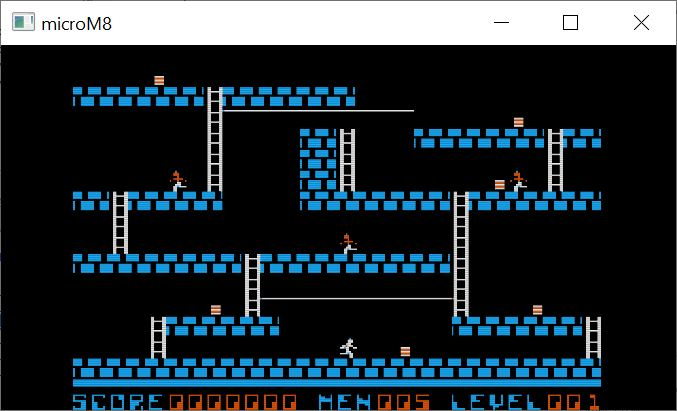
\includegraphics[width=\columnwidth]{screen}
\end{center}

There's a routine to add a 4-digit BCD
number to the score and then update it on the screen.

\nwenddocs{}\nwbegincode{58}\sublabel{NW1Xx3lK-8jv1b-D}\nwmargintag{{\nwtagstyle{}\subpageref{NW1Xx3lK-8jv1b-D}}}\moddef{routines~{\nwtagstyle{}\subpageref{NW1Xx3lK-8jv1b-1}}}\plusendmoddef\nwstartdeflinemarkup\nwusesondefline{\\{NW1Xx3lK-1p0Y9w-1}}\nwprevnextdefs{NW1Xx3lK-8jv1b-C}{NW1Xx3lK-8jv1b-E}\nwenddeflinemarkup
    ORG     $7A92
\nwlinkedidentc{ADD_AND_UPDATE_SCORE}{NW1Xx3lK-8jv1b-D}:
    SUBROUTINE
    ; Enter routine with A set to BCD tens/units and
    ; Y set to BCD thousands/hundreds.

    CLC
    SED                         ; Turn on BCD addition mode.
    ADC     \nwlinkedidentc{SCORE}{NW1Xx3lK-10jlgu-9}
    STA     \nwlinkedidentc{SCORE}{NW1Xx3lK-10jlgu-9}
    TYA
    ADC     \nwlinkedidentc{SCORE}{NW1Xx3lK-10jlgu-9}+1
    STA     \nwlinkedidentc{SCORE}{NW1Xx3lK-10jlgu-9}+1
    LDA     #$00
    ADC     \nwlinkedidentc{SCORE}{NW1Xx3lK-10jlgu-9}+2
    STA     \nwlinkedidentc{SCORE}{NW1Xx3lK-10jlgu-9}+2
    LDA     #$00
    ADC     \nwlinkedidentc{SCORE}{NW1Xx3lK-10jlgu-9}+3
    STA     \nwlinkedidentc{SCORE}{NW1Xx3lK-10jlgu-9}+3             ; \nwlinkedidentc{SCORE}{NW1Xx3lK-10jlgu-9} += param
    CLD                         ; Turn off BCD addition mode.

    LDA     5
    STA     \nwlinkedidentc{GAME_COLNUM}{NW1Xx3lK-10jlgu-5}
    LDA     16
    STA     \nwlinkedidentc{GAME_ROWNUM}{NW1Xx3lK-10jlgu-5}

    LDA     \nwlinkedidentc{SCORE}{NW1Xx3lK-10jlgu-9}+3
    JSR     \nwlinkedidentc{BCD_TO_DECIMAL2}{NW1Xx3lK-8jv1b-C}
    LDA     \nwlinkedidentc{UNITS}{NW1Xx3lK-10jlgu-8}               ; Note we skipped \nwlinkedidentc{TENS}{NW1Xx3lK-10jlgu-8}.
    JSR     \nwlinkedidentc{PUT_DIGIT}{NW1Xx3lK-8jv1b-A}

    LDA     \nwlinkedidentc{SCORE}{NW1Xx3lK-10jlgu-9}+2
    JSR     \nwlinkedidentc{BCD_TO_DECIMAL2}{NW1Xx3lK-8jv1b-C}
    LDA     \nwlinkedidentc{TENS}{NW1Xx3lK-10jlgu-8}
    JSR     \nwlinkedidentc{PUT_DIGIT}{NW1Xx3lK-8jv1b-A}
    LDA     \nwlinkedidentc{UNITS}{NW1Xx3lK-10jlgu-8}
    JSR     \nwlinkedidentc{PUT_DIGIT}{NW1Xx3lK-8jv1b-A}

    LDA     \nwlinkedidentc{SCORE}{NW1Xx3lK-10jlgu-9}+1
    JSR     \nwlinkedidentc{BCD_TO_DECIMAL2}{NW1Xx3lK-8jv1b-C}
    LDA     \nwlinkedidentc{TENS}{NW1Xx3lK-10jlgu-8}
    JSR     \nwlinkedidentc{PUT_DIGIT}{NW1Xx3lK-8jv1b-A}
    LDA     \nwlinkedidentc{UNITS}{NW1Xx3lK-10jlgu-8}
    JSR     \nwlinkedidentc{PUT_DIGIT}{NW1Xx3lK-8jv1b-A}

    LDA     \nwlinkedidentc{SCORE}{NW1Xx3lK-10jlgu-9}
    JSR     \nwlinkedidentc{BCD_TO_DECIMAL2}{NW1Xx3lK-8jv1b-C}
    LDA     \nwlinkedidentc{TENS}{NW1Xx3lK-10jlgu-8}
    JSR     \nwlinkedidentc{PUT_DIGIT}{NW1Xx3lK-8jv1b-A}
    LDA     \nwlinkedidentc{UNITS}{NW1Xx3lK-10jlgu-8}
    JMP     \nwlinkedidentc{PUT_DIGIT}{NW1Xx3lK-8jv1b-A}           ; tail call

\nwindexdefn{\nwixident{ADD{\_}AND{\_}UPDATE{\_}SCORE}}{ADD:unAND:unUPDATE:unSCORE}{NW1Xx3lK-8jv1b-D}\eatline
\nwused{\\{NW1Xx3lK-1p0Y9w-1}}\nwidentdefs{\\{{\nwixident{ADD{\_}AND{\_}UPDATE{\_}SCORE}}{ADD:unAND:unUPDATE:unSCORE}}}\nwidentuses{\\{{\nwixident{BCD{\_}TO{\_}DECIMAL2}}{BCD:unTO:unDECIMAL2}}\\{{\nwixident{GAME{\_}COLNUM}}{GAME:unCOLNUM}}\\{{\nwixident{GAME{\_}ROWNUM}}{GAME:unROWNUM}}\\{{\nwixident{PUT{\_}DIGIT}}{PUT:unDIGIT}}\\{{\nwixident{SCORE}}{SCORE}}\\{{\nwixident{TENS}}{TENS}}\\{{\nwixident{UNITS}}{UNITS}}}\nwindexuse{\nwixident{BCD{\_}TO{\_}DECIMAL2}}{BCD:unTO:unDECIMAL2}{NW1Xx3lK-8jv1b-D}\nwindexuse{\nwixident{GAME{\_}COLNUM}}{GAME:unCOLNUM}{NW1Xx3lK-8jv1b-D}\nwindexuse{\nwixident{GAME{\_}ROWNUM}}{GAME:unROWNUM}{NW1Xx3lK-8jv1b-D}\nwindexuse{\nwixident{PUT{\_}DIGIT}}{PUT:unDIGIT}{NW1Xx3lK-8jv1b-D}\nwindexuse{\nwixident{SCORE}}{SCORE}{NW1Xx3lK-8jv1b-D}\nwindexuse{\nwixident{TENS}}{TENS}{NW1Xx3lK-8jv1b-D}\nwindexuse{\nwixident{UNITS}}{UNITS}{NW1Xx3lK-8jv1b-D}\nwendcode{}\nwbegindocs{59}\nwdocspar
The other elements in the status line are the number of men
(i.e. lives) and the current level.

\nwenddocs{}\nwbegincode{60}\sublabel{NW1Xx3lK-10jlgu-A}\nwmargintag{{\nwtagstyle{}\subpageref{NW1Xx3lK-10jlgu-A}}}\moddef{defines~{\nwtagstyle{}\subpageref{NW1Xx3lK-10jlgu-1}}}\plusendmoddef\nwstartdeflinemarkup\nwusesondefline{\\{NW1Xx3lK-1p0Y9w-1}}\nwprevnextdefs{NW1Xx3lK-10jlgu-9}{NW1Xx3lK-10jlgu-B}\nwenddeflinemarkup
    ORG     $A6
\nwlinkedidentc{LEVELNUM}{NW1Xx3lK-10jlgu-A}    DS      1
    ORG     $C8
\nwlinkedidentc{LIVES}{NW1Xx3lK-10jlgu-A}       DS      1
\nwindexdefn{\nwixident{LEVELNUM}}{LEVELNUM}{NW1Xx3lK-10jlgu-A}\nwindexdefn{\nwixident{LIVES}}{LIVES}{NW1Xx3lK-10jlgu-A}\eatline
\nwused{\\{NW1Xx3lK-1p0Y9w-1}}\nwidentdefs{\\{{\nwixident{LEVELNUM}}{LEVELNUM}}\\{{\nwixident{LIVES}}{LIVES}}}\nwendcode{}\nwbegindocs{61}\nwdocspar
Here are the routines to put the lives and level number on
the status line. Lives starts at column 16, and level number
starts at column 25.

\nwenddocs{}\nwbegincode{62}\sublabel{NW1Xx3lK-8jv1b-E}\nwmargintag{{\nwtagstyle{}\subpageref{NW1Xx3lK-8jv1b-E}}}\moddef{routines~{\nwtagstyle{}\subpageref{NW1Xx3lK-8jv1b-1}}}\plusendmoddef\nwstartdeflinemarkup\nwusesondefline{\\{NW1Xx3lK-1p0Y9w-1}}\nwprevnextdefs{NW1Xx3lK-8jv1b-D}{NW1Xx3lK-8jv1b-F}\nwenddeflinemarkup
    ORG     $7a70
\nwlinkedidentc{PUT_STATUS_LIVES}{NW1Xx3lK-8jv1b-E}:
    SUBROUTINE

    LDA     \nwlinkedidentc{LIVES}{NW1Xx3lK-10jlgu-A}
    LDX     16
    ; fallthrough

PUT_STATUS_BYTE:
    SUBROUTINE
    ; Puts the number in A as a three-digit decimal on the screen
    ; at row 16, column X.

    STX     \nwlinkedidentc{GAME_COLNUM}{NW1Xx3lK-10jlgu-5}
    JSR     \nwlinkedidentc{TO_DECIMAL3}{NW1Xx3lK-8jv1b-B}
    LDA     16
    STA     \nwlinkedidentc{GAME_ROWNUM}{NW1Xx3lK-10jlgu-5}
    LDA     \nwlinkedidentc{HUNDREDS}{NW1Xx3lK-10jlgu-8}
    JSR     \nwlinkedidentc{PUT_DIGIT}{NW1Xx3lK-8jv1b-A}
    LDA     \nwlinkedidentc{TENS}{NW1Xx3lK-10jlgu-8}
    JSR     \nwlinkedidentc{PUT_DIGIT}{NW1Xx3lK-8jv1b-A}
    LDA     \nwlinkedidentc{UNITS}{NW1Xx3lK-10jlgu-8}
    JMP     \nwlinkedidentc{PUT_DIGIT}{NW1Xx3lK-8jv1b-A}           ; tail call

\nwlinkedidentc{PUT_STATUS_LEVEL}{NW1Xx3lK-8jv1b-E}:
    SUBROUTINE

    LDA     \nwlinkedidentc{LEVELNUM}{NW1Xx3lK-10jlgu-A}
    LDX     25
    BNE     PUT_STATUS_BYTE     ; Unconditional jump

\nwindexdefn{\nwixident{PUT{\_}STATUS{\_}LIVES}}{PUT:unSTATUS:unLIVES}{NW1Xx3lK-8jv1b-E}\nwindexdefn{\nwixident{PUT{\_}STATUS{\_}LEVEL}}{PUT:unSTATUS:unLEVEL}{NW1Xx3lK-8jv1b-E}\eatline
\nwused{\\{NW1Xx3lK-1p0Y9w-1}}\nwidentdefs{\\{{\nwixident{PUT{\_}STATUS{\_}LEVEL}}{PUT:unSTATUS:unLEVEL}}\\{{\nwixident{PUT{\_}STATUS{\_}LIVES}}{PUT:unSTATUS:unLIVES}}}\nwidentuses{\\{{\nwixident{GAME{\_}COLNUM}}{GAME:unCOLNUM}}\\{{\nwixident{GAME{\_}ROWNUM}}{GAME:unROWNUM}}\\{{\nwixident{HUNDREDS}}{HUNDREDS}}\\{{\nwixident{LEVELNUM}}{LEVELNUM}}\\{{\nwixident{LIVES}}{LIVES}}\\{{\nwixident{PUT{\_}DIGIT}}{PUT:unDIGIT}}\\{{\nwixident{TENS}}{TENS}}\\{{\nwixident{TO{\_}DECIMAL3}}{TO:unDECIMAL3}}\\{{\nwixident{UNITS}}{UNITS}}}\nwindexuse{\nwixident{GAME{\_}COLNUM}}{GAME:unCOLNUM}{NW1Xx3lK-8jv1b-E}\nwindexuse{\nwixident{GAME{\_}ROWNUM}}{GAME:unROWNUM}{NW1Xx3lK-8jv1b-E}\nwindexuse{\nwixident{HUNDREDS}}{HUNDREDS}{NW1Xx3lK-8jv1b-E}\nwindexuse{\nwixident{LEVELNUM}}{LEVELNUM}{NW1Xx3lK-8jv1b-E}\nwindexuse{\nwixident{LIVES}}{LIVES}{NW1Xx3lK-8jv1b-E}\nwindexuse{\nwixident{PUT{\_}DIGIT}}{PUT:unDIGIT}{NW1Xx3lK-8jv1b-E}\nwindexuse{\nwixident{TENS}}{TENS}{NW1Xx3lK-8jv1b-E}\nwindexuse{\nwixident{TO{\_}DECIMAL3}}{TO:unDECIMAL3}{NW1Xx3lK-8jv1b-E}\nwindexuse{\nwixident{UNITS}}{UNITS}{NW1Xx3lK-8jv1b-E}\nwendcode{}\nwbegindocs{63}\nwdocspar
\chapter{Levels}

One of the appealing things about Lode Runner are its levels. 150 levels are stored
in the game, and there is even a level editor included.

\section{Drawing a level}

Let's see how Lode Runner draws a level. We start with the routine {\Tt{}\nwlinkedidentq{DRAW{\_}LEVEL{\_}PAGE2}{NW1Xx3lK-2Mcso2-1}\nwendquote},
which draws a level on HGR2. Note that HGR1 would be displayed, so the player doesn't
see the draw happening.

We start by looping backwards over rows 15 through 0:

\nwenddocs{}\nwbegincode{64}\sublabel{NW1Xx3lK-2Mcso2-1}\nwmargintag{{\nwtagstyle{}\subpageref{NW1Xx3lK-2Mcso2-1}}}\moddef{level draw routine~{\nwtagstyle{}\subpageref{NW1Xx3lK-2Mcso2-1}}}\endmoddef\nwstartdeflinemarkup\nwusesondefline{\\{NW1Xx3lK-8jv1b-F}}\nwprevnextdefs{\relax}{NW1Xx3lK-2Mcso2-2}\nwenddeflinemarkup
    ORG     $63B3
\nwlinkedidentc{DRAW_LEVEL_PAGE2}{NW1Xx3lK-2Mcso2-1}:
    SUBROUTINE

    LDY     15
    STY     \nwlinkedidentc{GAME_ROWNUM}{NW1Xx3lK-10jlgu-5}

.row_loop:
\nwindexdefn{\nwixident{DRAW{\_}LEVEL{\_}PAGE2}}{DRAW:unLEVEL:unPAGE2}{NW1Xx3lK-2Mcso2-1}\eatline
\nwalsodefined{\\{NW1Xx3lK-2Mcso2-2}\\{NW1Xx3lK-2Mcso2-3}\\{NW1Xx3lK-2Mcso2-4}\\{NW1Xx3lK-2Mcso2-5}\\{NW1Xx3lK-2Mcso2-6}\\{NW1Xx3lK-2Mcso2-7}\\{NW1Xx3lK-2Mcso2-8}\\{NW1Xx3lK-2Mcso2-9}\\{NW1Xx3lK-2Mcso2-A}\\{NW1Xx3lK-2Mcso2-B}\\{NW1Xx3lK-2Mcso2-C}\\{NW1Xx3lK-2Mcso2-D}\\{NW1Xx3lK-2Mcso2-E}\\{NW1Xx3lK-2Mcso2-F}\\{NW1Xx3lK-2Mcso2-G}}\nwused{\\{NW1Xx3lK-8jv1b-F}}\nwidentdefs{\\{{\nwixident{DRAW{\_}LEVEL{\_}PAGE2}}{DRAW:unLEVEL:unPAGE2}}}\nwidentuses{\\{{\nwixident{GAME{\_}ROWNUM}}{GAME:unROWNUM}}}\nwindexuse{\nwixident{GAME{\_}ROWNUM}}{GAME:unROWNUM}{NW1Xx3lK-2Mcso2-1}\nwendcode{}\nwbegindocs{65}\nwdocspar
We'll assume the level data is stored in
a table which contains 16 pointers, one for each row. As usual in Lode Runner,
the pages and offsets for those pointers are stored in separate tables. these
are {\Tt{}\nwlinkedidentq{CURR{\_}LEVEL{\_}ROW{\_}SPRITES{\_}PTR{\_}PAGES}{NW1Xx3lK-1W8AJS-8}\nwendquote} and {\Tt{}\nwlinkedidentq{CURR{\_}LEVEL{\_}ROW{\_}SPRITES{\_}PTR{\_}OFFSETS}{NW1Xx3lK-1W8AJS-8}\nwendquote}.

\nwenddocs{}\nwbegincode{66}\sublabel{NW1Xx3lK-1W8AJS-8}\nwmargintag{{\nwtagstyle{}\subpageref{NW1Xx3lK-1W8AJS-8}}}\moddef{tables~{\nwtagstyle{}\subpageref{NW1Xx3lK-1W8AJS-1}}}\plusendmoddef\nwstartdeflinemarkup\nwusesondefline{\\{NW1Xx3lK-1p0Y9w-1}}\nwprevnextdefs{NW1Xx3lK-1W8AJS-7}{NW1Xx3lK-1W8AJS-9}\nwenddeflinemarkup
    ORG     $1C05
\nwlinkedidentc{CURR_LEVEL_ROW_SPRITES_PTR_OFFSETS}{NW1Xx3lK-1W8AJS-8}:
    HEX     00 1C 38 54 70 8C A8 C4 E0 FC 18 34 50 6C 88 A4
\nwlinkedidentc{CURR_LEVEL_ROW_SPRITES_PTR_PAGES}{NW1Xx3lK-1W8AJS-8}:
    HEX     08 08 08 08 08 08 08 08 08 08 09 09 09 09 09 09
\nwlinkedidentc{CURR_LEVEL_ROW_SPRITES_PTR_PAGES2}{NW1Xx3lK-1W8AJS-8}:
    HEX     0A 0A 0A 0A 0A 0A 0A 0A 0A 0A 0B 0B 0B 0B 0B 0B
\nwindexdefn{\nwixident{CURR{\_}LEVEL{\_}ROW{\_}SPRITES{\_}PTR{\_}OFFSETS}}{CURR:unLEVEL:unROW:unSPRITES:unPTR:unOFFSETS}{NW1Xx3lK-1W8AJS-8}\nwindexdefn{\nwixident{CURR{\_}LEVEL{\_}ROW{\_}SPRITES{\_}PTR{\_}PAGES}}{CURR:unLEVEL:unROW:unSPRITES:unPTR:unPAGES}{NW1Xx3lK-1W8AJS-8}\nwindexdefn{\nwixident{CURR{\_}LEVEL{\_}ROW{\_}SPRITES{\_}PTR{\_}PAGES2}}{CURR:unLEVEL:unROW:unSPRITES:unPTR:unPAGES2}{NW1Xx3lK-1W8AJS-8}\eatline
\nwused{\\{NW1Xx3lK-1p0Y9w-1}}\nwidentdefs{\\{{\nwixident{CURR{\_}LEVEL{\_}ROW{\_}SPRITES{\_}PTR{\_}OFFSETS}}{CURR:unLEVEL:unROW:unSPRITES:unPTR:unOFFSETS}}\\{{\nwixident{CURR{\_}LEVEL{\_}ROW{\_}SPRITES{\_}PTR{\_}PAGES}}{CURR:unLEVEL:unROW:unSPRITES:unPTR:unPAGES}}\\{{\nwixident{CURR{\_}LEVEL{\_}ROW{\_}SPRITES{\_}PTR{\_}PAGES2}}{CURR:unLEVEL:unROW:unSPRITES:unPTR:unPAGES2}}}\nwendcode{}\nwbegindocs{67}\nwdocspar
At the beginning of this loop, we create two pointers which we'll simply
call {\Tt{}\nwlinkedidentq{PTR1}{NW1Xx3lK-10jlgu-B}\nwendquote} and {\Tt{}\nwlinkedidentq{PTR2}{NW1Xx3lK-10jlgu-B}\nwendquote}. 

\nwenddocs{}\nwbegincode{68}\sublabel{NW1Xx3lK-10jlgu-B}\nwmargintag{{\nwtagstyle{}\subpageref{NW1Xx3lK-10jlgu-B}}}\moddef{defines~{\nwtagstyle{}\subpageref{NW1Xx3lK-10jlgu-1}}}\plusendmoddef\nwstartdeflinemarkup\nwusesondefline{\\{NW1Xx3lK-1p0Y9w-1}}\nwprevnextdefs{NW1Xx3lK-10jlgu-A}{NW1Xx3lK-10jlgu-C}\nwenddeflinemarkup
\nwlinkedidentc{PTR1}{NW1Xx3lK-10jlgu-B}        EQU     $06     ; 2 bytes
\nwlinkedidentc{PTR2}{NW1Xx3lK-10jlgu-B}        EQU     $08     ; 2 bytes
\nwindexdefn{\nwixident{PTR1}}{PTR1}{NW1Xx3lK-10jlgu-B}\nwindexdefn{\nwixident{PTR2}}{PTR2}{NW1Xx3lK-10jlgu-B}\eatline
\nwused{\\{NW1Xx3lK-1p0Y9w-1}}\nwidentdefs{\\{{\nwixident{PTR1}}{PTR1}}\\{{\nwixident{PTR2}}{PTR2}}}\nwendcode{}\nwbegindocs{69}\nwdocspar
We set {\Tt{}\nwlinkedidentq{PTR1}{NW1Xx3lK-10jlgu-B}\nwendquote} to the pointer corresponding to the current row, and {\Tt{}\nwlinkedidentq{PTR2}{NW1Xx3lK-10jlgu-B}\nwendquote} to the other
page, though I don't know what it's for yet.

\nwenddocs{}\nwbegincode{70}\sublabel{NW1Xx3lK-2Mcso2-2}\nwmargintag{{\nwtagstyle{}\subpageref{NW1Xx3lK-2Mcso2-2}}}\moddef{level draw routine~{\nwtagstyle{}\subpageref{NW1Xx3lK-2Mcso2-1}}}\plusendmoddef\nwstartdeflinemarkup\nwusesondefline{\\{NW1Xx3lK-8jv1b-F}}\nwprevnextdefs{NW1Xx3lK-2Mcso2-1}{NW1Xx3lK-2Mcso2-3}\nwenddeflinemarkup
    LDA     \nwlinkedidentc{CURR_LEVEL_ROW_SPRITES_PTR_OFFSETS}{NW1Xx3lK-1W8AJS-8},Y
    STA     \nwlinkedidentc{PTR1}{NW1Xx3lK-10jlgu-B}
    STA     \nwlinkedidentc{PTR2}{NW1Xx3lK-10jlgu-B}
    LDA     \nwlinkedidentc{CURR_LEVEL_ROW_SPRITES_PTR_PAGES}{NW1Xx3lK-1W8AJS-8},Y
    STA     \nwlinkedidentc{PTR1}{NW1Xx3lK-10jlgu-B}+1
    LDA     \nwlinkedidentc{CURR_LEVEL_ROW_SPRITES_PTR_PAGES2}{NW1Xx3lK-1W8AJS-8},Y
    STA     \nwlinkedidentc{PTR2}{NW1Xx3lK-10jlgu-B}+1
\nwused{\\{NW1Xx3lK-8jv1b-F}}\nwidentuses{\\{{\nwixident{CURR{\_}LEVEL{\_}ROW{\_}SPRITES{\_}PTR{\_}OFFSETS}}{CURR:unLEVEL:unROW:unSPRITES:unPTR:unOFFSETS}}\\{{\nwixident{CURR{\_}LEVEL{\_}ROW{\_}SPRITES{\_}PTR{\_}PAGES}}{CURR:unLEVEL:unROW:unSPRITES:unPTR:unPAGES}}\\{{\nwixident{CURR{\_}LEVEL{\_}ROW{\_}SPRITES{\_}PTR{\_}PAGES2}}{CURR:unLEVEL:unROW:unSPRITES:unPTR:unPAGES2}}\\{{\nwixident{PTR1}}{PTR1}}\\{{\nwixident{PTR2}}{PTR2}}}\nwindexuse{\nwixident{CURR{\_}LEVEL{\_}ROW{\_}SPRITES{\_}PTR{\_}OFFSETS}}{CURR:unLEVEL:unROW:unSPRITES:unPTR:unOFFSETS}{NW1Xx3lK-2Mcso2-2}\nwindexuse{\nwixident{CURR{\_}LEVEL{\_}ROW{\_}SPRITES{\_}PTR{\_}PAGES}}{CURR:unLEVEL:unROW:unSPRITES:unPTR:unPAGES}{NW1Xx3lK-2Mcso2-2}\nwindexuse{\nwixident{CURR{\_}LEVEL{\_}ROW{\_}SPRITES{\_}PTR{\_}PAGES2}}{CURR:unLEVEL:unROW:unSPRITES:unPTR:unPAGES2}{NW1Xx3lK-2Mcso2-2}\nwindexuse{\nwixident{PTR1}}{PTR1}{NW1Xx3lK-2Mcso2-2}\nwindexuse{\nwixident{PTR2}}{PTR2}{NW1Xx3lK-2Mcso2-2}\nwendcode{}\nwbegindocs{71}\nwdocspar

Next, we loop over the columns backwards from 27 to 0.

\nwenddocs{}\nwbegincode{72}\sublabel{NW1Xx3lK-2Mcso2-3}\nwmargintag{{\nwtagstyle{}\subpageref{NW1Xx3lK-2Mcso2-3}}}\moddef{level draw routine~{\nwtagstyle{}\subpageref{NW1Xx3lK-2Mcso2-1}}}\plusendmoddef\nwstartdeflinemarkup\nwusesondefline{\\{NW1Xx3lK-8jv1b-F}}\nwprevnextdefs{NW1Xx3lK-2Mcso2-2}{NW1Xx3lK-2Mcso2-4}\nwenddeflinemarkup
    LDY     27
    STY     \nwlinkedidentc{GAME_COLNUM}{NW1Xx3lK-10jlgu-5}

.col_loop:
\nwused{\\{NW1Xx3lK-8jv1b-F}}\nwidentuses{\\{{\nwixident{GAME{\_}COLNUM}}{GAME:unCOLNUM}}}\nwindexuse{\nwixident{GAME{\_}COLNUM}}{GAME:unCOLNUM}{NW1Xx3lK-2Mcso2-3}\nwendcode{}\nwbegindocs{73}\nwdocspar

We load the sprite from the level data.

\nwenddocs{}\nwbegincode{74}\sublabel{NW1Xx3lK-2Mcso2-4}\nwmargintag{{\nwtagstyle{}\subpageref{NW1Xx3lK-2Mcso2-4}}}\moddef{level draw routine~{\nwtagstyle{}\subpageref{NW1Xx3lK-2Mcso2-1}}}\plusendmoddef\nwstartdeflinemarkup\nwusesondefline{\\{NW1Xx3lK-8jv1b-F}}\nwprevnextdefs{NW1Xx3lK-2Mcso2-3}{NW1Xx3lK-2Mcso2-5}\nwenddeflinemarkup
    LDA     (\nwlinkedidentc{PTR1}{NW1Xx3lK-10jlgu-B}),Y
\nwused{\\{NW1Xx3lK-8jv1b-F}}\nwidentuses{\\{{\nwixident{PTR1}}{PTR1}}}\nwindexuse{\nwixident{PTR1}}{PTR1}{NW1Xx3lK-2Mcso2-4}\nwendcode{}\nwbegindocs{75}\nwdocspar

Now, as we place each sprite, we count the number of each piece we've used so far.
Remember that anyone can create a level, but there are some limitations. Specifically,
we are limited to 45 ladders, one player, and 5 guards. We store the counts
as we go.

We'll assume that these values are zeroed before the {\Tt{}\nwlinkedidentq{DRAW{\_}LEVEL{\_}PAGE2}{NW1Xx3lK-2Mcso2-1}\nwendquote} routine is called.

\nwenddocs{}\nwbegincode{76}\sublabel{NW1Xx3lK-10jlgu-C}\nwmargintag{{\nwtagstyle{}\subpageref{NW1Xx3lK-10jlgu-C}}}\moddef{defines~{\nwtagstyle{}\subpageref{NW1Xx3lK-10jlgu-1}}}\plusendmoddef\nwstartdeflinemarkup\nwusesondefline{\\{NW1Xx3lK-1p0Y9w-1}}\nwprevnextdefs{NW1Xx3lK-10jlgu-B}{NW1Xx3lK-10jlgu-D}\nwenddeflinemarkup
    ORG     $00
\nwlinkedidentc{PLAYER_COL}{NW1Xx3lK-10jlgu-C}      DS      1       ; The column number of the player.
\nwlinkedidentc{PLAYER_ROW}{NW1Xx3lK-10jlgu-C}      DS      1       ; The row number of the player.
    ORG     $8D
\nwlinkedidentc{GUARD_COUNT}{NW1Xx3lK-10jlgu-C}     DS      1
    ORG     $93
\nwlinkedidentc{GOLD_COUNT}{NW1Xx3lK-10jlgu-C}      DS      1
    ORG     $A3
\nwlinkedidentc{LADDER_COUNT}{NW1Xx3lK-10jlgu-C}    DS      1
\nwindexdefn{\nwixident{PLAYER{\_}COL}}{PLAYER:unCOL}{NW1Xx3lK-10jlgu-C}\nwindexdefn{\nwixident{PLAYER{\_}ROW}}{PLAYER:unROW}{NW1Xx3lK-10jlgu-C}\nwindexdefn{\nwixident{GUARD{\_}COUNT}}{GUARD:unCOUNT}{NW1Xx3lK-10jlgu-C}\nwindexdefn{\nwixident{GOLD{\_}COUNT}}{GOLD:unCOUNT}{NW1Xx3lK-10jlgu-C}\nwindexdefn{\nwixident{LADDER{\_}COUNT}}{LADDER:unCOUNT}{NW1Xx3lK-10jlgu-C}\eatline
\nwused{\\{NW1Xx3lK-1p0Y9w-1}}\nwidentdefs{\\{{\nwixident{GOLD{\_}COUNT}}{GOLD:unCOUNT}}\\{{\nwixident{GUARD{\_}COUNT}}{GUARD:unCOUNT}}\\{{\nwixident{LADDER{\_}COUNT}}{LADDER:unCOUNT}}\\{{\nwixident{PLAYER{\_}COL}}{PLAYER:unCOL}}\\{{\nwixident{PLAYER{\_}ROW}}{PLAYER:unROW}}}\nwendcode{}\nwbegindocs{77}\nwdocspar
However, there's a flag called {\Tt{}\nwlinkedidentq{VERBATIM}{NW1Xx3lK-10jlgu-D}\nwendquote} that tells us whether we want to ignore
these counts and just draw the level as specified. Possibly when we're using the
level editor.

\nwenddocs{}\nwbegincode{78}\sublabel{NW1Xx3lK-10jlgu-D}\nwmargintag{{\nwtagstyle{}\subpageref{NW1Xx3lK-10jlgu-D}}}\moddef{defines~{\nwtagstyle{}\subpageref{NW1Xx3lK-10jlgu-1}}}\plusendmoddef\nwstartdeflinemarkup\nwusesondefline{\\{NW1Xx3lK-1p0Y9w-1}}\nwprevnextdefs{NW1Xx3lK-10jlgu-C}{NW1Xx3lK-10jlgu-E}\nwenddeflinemarkup
    ORG     $A2
\nwlinkedidentc{VERBATIM}{NW1Xx3lK-10jlgu-D}        DS      1
\nwindexdefn{\nwixident{VERBATIM}}{VERBATIM}{NW1Xx3lK-10jlgu-D}\eatline
\nwused{\\{NW1Xx3lK-1p0Y9w-1}}\nwidentdefs{\\{{\nwixident{VERBATIM}}{VERBATIM}}}\nwendcode{}\nwbegindocs{79}\nwdocspar
\nwenddocs{}\nwbegincode{80}\sublabel{NW1Xx3lK-2Mcso2-5}\nwmargintag{{\nwtagstyle{}\subpageref{NW1Xx3lK-2Mcso2-5}}}\moddef{level draw routine~{\nwtagstyle{}\subpageref{NW1Xx3lK-2Mcso2-1}}}\plusendmoddef\nwstartdeflinemarkup\nwusesondefline{\\{NW1Xx3lK-8jv1b-F}}\nwprevnextdefs{NW1Xx3lK-2Mcso2-4}{NW1Xx3lK-2Mcso2-6}\nwenddeflinemarkup
    LDX     \nwlinkedidentc{VERBATIM}{NW1Xx3lK-10jlgu-D}
    BEQ     .draw_sprite1       ; This will then unconditionally jump to
                                ; .draw_sprite2. We have to do that because of
                                ; relative jump amount limitations.
\nwused{\\{NW1Xx3lK-8jv1b-F}}\nwidentuses{\\{{\nwixident{VERBATIM}}{VERBATIM}}}\nwindexuse{\nwixident{VERBATIM}}{VERBATIM}{NW1Xx3lK-2Mcso2-5}\nwendcode{}\nwbegindocs{81}\nwdocspar

Next we handle sprite 6, which is a symbol used to denote ladder placement. If we've already
got the maximum number of ladders, we just put in a space instead. For each ladder placed, we
write the {\Tt{}LADDER{\_}LOCS\nwendquote} table with its coordinates.

\nwenddocs{}\nwbegincode{82}\sublabel{NW1Xx3lK-1W8AJS-9}\nwmargintag{{\nwtagstyle{}\subpageref{NW1Xx3lK-1W8AJS-9}}}\moddef{tables~{\nwtagstyle{}\subpageref{NW1Xx3lK-1W8AJS-1}}}\plusendmoddef\nwstartdeflinemarkup\nwusesondefline{\\{NW1Xx3lK-1p0Y9w-1}}\nwprevnextdefs{NW1Xx3lK-1W8AJS-8}{NW1Xx3lK-1W8AJS-A}\nwenddeflinemarkup
    ORG     $0C00
\nwlinkedidentc{LADDER_LOCS_COL}{NW1Xx3lK-1W8AJS-9}     DS      48
\nwlinkedidentc{LADDER_LOCS_ROW}{NW1Xx3lK-1W8AJS-9}     DS      48
\nwindexdefn{\nwixident{LADDER{\_}LOCS{\_}COL}}{LADDER:unLOCS:unCOL}{NW1Xx3lK-1W8AJS-9}\nwindexdefn{\nwixident{LADDER{\_}LOCS{\_}ROW}}{LADDER:unLOCS:unROW}{NW1Xx3lK-1W8AJS-9}\eatline
\nwused{\\{NW1Xx3lK-1p0Y9w-1}}\nwidentdefs{\\{{\nwixident{LADDER{\_}LOCS{\_}COL}}{LADDER:unLOCS:unCOL}}\\{{\nwixident{LADDER{\_}LOCS{\_}ROW}}{LADDER:unLOCS:unROW}}}\nwendcode{}\nwbegindocs{83}\nwdocspar
\nwenddocs{}\nwbegincode{84}\sublabel{NW1Xx3lK-2Mcso2-6}\nwmargintag{{\nwtagstyle{}\subpageref{NW1Xx3lK-2Mcso2-6}}}\moddef{level draw routine~{\nwtagstyle{}\subpageref{NW1Xx3lK-2Mcso2-1}}}\plusendmoddef\nwstartdeflinemarkup\nwusesondefline{\\{NW1Xx3lK-8jv1b-F}}\nwprevnextdefs{NW1Xx3lK-2Mcso2-5}{NW1Xx3lK-2Mcso2-7}\nwenddeflinemarkup
    CMP      #$06
    BNE     .check_for_box

    LDX     \nwlinkedidentc{LADDER_COUNT}{NW1Xx3lK-10jlgu-C}
    CPX     45
    BCS     .remove_sprite

    INC     \nwlinkedidentc{LADDER_COUNT}{NW1Xx3lK-10jlgu-C}
    INX
    LDA     \nwlinkedidentc{GAME_ROWNUM}{NW1Xx3lK-10jlgu-5}
    STA     \nwlinkedidentc{LADDER_LOCS_ROW}{NW1Xx3lK-1W8AJS-9},X
    TYA
    STA     \nwlinkedidentc{LADDER_LOCS_COL}{NW1Xx3lK-1W8AJS-9},X

\nwused{\\{NW1Xx3lK-8jv1b-F}}\nwidentuses{\\{{\nwixident{GAME{\_}ROWNUM}}{GAME:unROWNUM}}\\{{\nwixident{LADDER{\_}COUNT}}{LADDER:unCOUNT}}\\{{\nwixident{LADDER{\_}LOCS{\_}COL}}{LADDER:unLOCS:unCOL}}\\{{\nwixident{LADDER{\_}LOCS{\_}ROW}}{LADDER:unLOCS:unROW}}}\nwindexuse{\nwixident{GAME{\_}ROWNUM}}{GAME:unROWNUM}{NW1Xx3lK-2Mcso2-6}\nwindexuse{\nwixident{LADDER{\_}COUNT}}{LADDER:unCOUNT}{NW1Xx3lK-2Mcso2-6}\nwindexuse{\nwixident{LADDER{\_}LOCS{\_}COL}}{LADDER:unLOCS:unCOL}{NW1Xx3lK-2Mcso2-6}\nwindexuse{\nwixident{LADDER{\_}LOCS{\_}ROW}}{LADDER:unLOCS:unROW}{NW1Xx3lK-2Mcso2-6}\nwendcode{}\nwbegindocs{85}\nwdocspar

In any case, we remove the sprite from the current level data.

\nwenddocs{}\nwbegincode{86}\sublabel{NW1Xx3lK-2Mcso2-7}\nwmargintag{{\nwtagstyle{}\subpageref{NW1Xx3lK-2Mcso2-7}}}\moddef{level draw routine~{\nwtagstyle{}\subpageref{NW1Xx3lK-2Mcso2-1}}}\plusendmoddef\nwstartdeflinemarkup\nwusesondefline{\\{NW1Xx3lK-8jv1b-F}}\nwprevnextdefs{NW1Xx3lK-2Mcso2-6}{NW1Xx3lK-2Mcso2-8}\nwenddeflinemarkup
.remove_sprite:
    LDA     0
    STA     (\nwlinkedidentc{PTR1}{NW1Xx3lK-10jlgu-B}),Y
    STA     (\nwlinkedidentc{PTR2}{NW1Xx3lK-10jlgu-B}),Y

.draw_sprite1
    BEQ     .draw_sprite        ; Unconditional jump.
\nwused{\\{NW1Xx3lK-8jv1b-F}}\nwidentuses{\\{{\nwixident{PTR1}}{PTR1}}\\{{\nwixident{PTR2}}{PTR2}}}\nwindexuse{\nwixident{PTR1}}{PTR1}{NW1Xx3lK-2Mcso2-7}\nwindexuse{\nwixident{PTR2}}{PTR2}{NW1Xx3lK-2Mcso2-7}\nwendcode{}\nwbegindocs{87}\nwdocspar

Next, we check for sprite 7, the gold box.

\nwenddocs{}\nwbegincode{88}\sublabel{NW1Xx3lK-2Mcso2-8}\nwmargintag{{\nwtagstyle{}\subpageref{NW1Xx3lK-2Mcso2-8}}}\moddef{level draw routine~{\nwtagstyle{}\subpageref{NW1Xx3lK-2Mcso2-1}}}\plusendmoddef\nwstartdeflinemarkup\nwusesondefline{\\{NW1Xx3lK-8jv1b-F}}\nwprevnextdefs{NW1Xx3lK-2Mcso2-7}{NW1Xx3lK-2Mcso2-9}\nwenddeflinemarkup
.check_for_box:
    CMP      #$07
    BNE     .check_for_8

    INC     \nwlinkedidentc{GOLD_COUNT}{NW1Xx3lK-10jlgu-C}
    BNE     .draw_sprite        ; This leads to a situation where if we wrap
                                ; \nwlinkedidentc{GOLD_COUNT}{NW1Xx3lK-10jlgu-C} around back to 0 (so 256 boxes)
                                ; we end up falling through, which eventually
                                ; just draws the sprite anyway. So this is kind
                                ; of unconditional.

\nwused{\\{NW1Xx3lK-8jv1b-F}}\nwidentuses{\\{{\nwixident{GOLD{\_}COUNT}}{GOLD:unCOUNT}}}\nwindexuse{\nwixident{GOLD{\_}COUNT}}{GOLD:unCOUNT}{NW1Xx3lK-2Mcso2-8}\nwendcode{}\nwbegindocs{89}\nwdocspar

Next, we check for sprite 8, a guard. If we've already
got the maximum number of guards, we just put in a space instead. For each guard placed, we
write the {\Tt{}GUARD{\_}LOCS\nwendquote} table with its coordinates. We also write some other guard-related
tables.

\nwenddocs{}\nwbegincode{90}\sublabel{NW1Xx3lK-1W8AJS-A}\nwmargintag{{\nwtagstyle{}\subpageref{NW1Xx3lK-1W8AJS-A}}}\moddef{tables~{\nwtagstyle{}\subpageref{NW1Xx3lK-1W8AJS-1}}}\plusendmoddef\nwstartdeflinemarkup\nwusesondefline{\\{NW1Xx3lK-1p0Y9w-1}}\nwprevnextdefs{NW1Xx3lK-1W8AJS-9}{NW1Xx3lK-1W8AJS-B}\nwenddeflinemarkup
    ORG     $0C60
\nwlinkedidentc{GUARD_LOCS_COL}{NW1Xx3lK-1W8AJS-A}      DS      8
\nwlinkedidentc{GUARD_LOCS_ROW}{NW1Xx3lK-1W8AJS-A}      DS      8
\nwlinkedidentc{GUARD_FLAGS_0C70}{NW1Xx3lK-1W8AJS-A}    DS      8
\nwlinkedidentc{GUARD_FLAGS_0C78}{NW1Xx3lK-1W8AJS-A}    DS      8
\nwlinkedidentc{GUARD_FLAGS_0C80}{NW1Xx3lK-1W8AJS-A}    DS      8
\nwlinkedidentc{GUARD_FLAGS_0C88}{NW1Xx3lK-1W8AJS-A}    DS      8
\nwindexdefn{\nwixident{GUARD{\_}LOCS{\_}COL}}{GUARD:unLOCS:unCOL}{NW1Xx3lK-1W8AJS-A}\nwindexdefn{\nwixident{GUARD{\_}LOCS{\_}ROW}}{GUARD:unLOCS:unROW}{NW1Xx3lK-1W8AJS-A}\nwindexdefn{\nwixident{GUARD{\_}FLAGS{\_}0C70}}{GUARD:unFLAGS:un0C70}{NW1Xx3lK-1W8AJS-A}\nwindexdefn{\nwixident{GUARD{\_}FLAGS{\_}0C78}}{GUARD:unFLAGS:un0C78}{NW1Xx3lK-1W8AJS-A}\nwindexdefn{\nwixident{GUARD{\_}FLAGS{\_}0C80}}{GUARD:unFLAGS:un0C80}{NW1Xx3lK-1W8AJS-A}\nwindexdefn{\nwixident{GUARD{\_}FLAGS{\_}0C88}}{GUARD:unFLAGS:un0C88}{NW1Xx3lK-1W8AJS-A}\eatline
\nwused{\\{NW1Xx3lK-1p0Y9w-1}}\nwidentdefs{\\{{\nwixident{GUARD{\_}FLAGS{\_}0C70}}{GUARD:unFLAGS:un0C70}}\\{{\nwixident{GUARD{\_}FLAGS{\_}0C78}}{GUARD:unFLAGS:un0C78}}\\{{\nwixident{GUARD{\_}FLAGS{\_}0C80}}{GUARD:unFLAGS:un0C80}}\\{{\nwixident{GUARD{\_}FLAGS{\_}0C88}}{GUARD:unFLAGS:un0C88}}\\{{\nwixident{GUARD{\_}LOCS{\_}COL}}{GUARD:unLOCS:unCOL}}\\{{\nwixident{GUARD{\_}LOCS{\_}ROW}}{GUARD:unLOCS:unROW}}}\nwendcode{}\nwbegindocs{91}\nwdocspar
\nwenddocs{}\nwbegincode{92}\sublabel{NW1Xx3lK-2Mcso2-9}\nwmargintag{{\nwtagstyle{}\subpageref{NW1Xx3lK-2Mcso2-9}}}\moddef{level draw routine~{\nwtagstyle{}\subpageref{NW1Xx3lK-2Mcso2-1}}}\plusendmoddef\nwstartdeflinemarkup\nwusesondefline{\\{NW1Xx3lK-8jv1b-F}}\nwprevnextdefs{NW1Xx3lK-2Mcso2-8}{NW1Xx3lK-2Mcso2-A}\nwenddeflinemarkup
.check_for_8:
    CMP     #$08
    BNE     .check_for_9

    LDX     \nwlinkedidentc{GUARD_COUNT}{NW1Xx3lK-10jlgu-C}
    CPX     5
    BCS     .remove_sprite          ; If \nwlinkedidentc{GUARD_COUNT}{NW1Xx3lK-10jlgu-C} > 5, remove sprite.

    INC     \nwlinkedidentc{GUARD_COUNT}{NW1Xx3lK-10jlgu-C}
    INX
    TYA
    STA     \nwlinkedidentc{GUARD_LOCS_COL}{NW1Xx3lK-1W8AJS-A},X
    LDA     \nwlinkedidentc{GAME_ROWNUM}{NW1Xx3lK-10jlgu-5}
    STA     \nwlinkedidentc{GUARD_LOCS_ROW}{NW1Xx3lK-1W8AJS-A},X
    LDA     #$00
    STA     \nwlinkedidentc{GUARD_FLAGS_0C70}{NW1Xx3lK-1W8AJS-A},X
    STA     \nwlinkedidentc{GUARD_FLAGS_0C88}{NW1Xx3lK-1W8AJS-A},X
    LDA     #$02
    STA     \nwlinkedidentc{GUARD_FLAGS_0C78}{NW1Xx3lK-1W8AJS-A},X
    STA     \nwlinkedidentc{GUARD_FLAGS_0C80}{NW1Xx3lK-1W8AJS-A},X

    LDA     #$00
    STA     (\nwlinkedidentc{PTR2}{NW1Xx3lK-10jlgu-B}),Y
    LDA     #$08
    BNE     .draw_sprite            ; Unconditional jump.

\nwused{\\{NW1Xx3lK-8jv1b-F}}\nwidentuses{\\{{\nwixident{GAME{\_}ROWNUM}}{GAME:unROWNUM}}\\{{\nwixident{GUARD{\_}COUNT}}{GUARD:unCOUNT}}\\{{\nwixident{GUARD{\_}FLAGS{\_}0C70}}{GUARD:unFLAGS:un0C70}}\\{{\nwixident{GUARD{\_}FLAGS{\_}0C78}}{GUARD:unFLAGS:un0C78}}\\{{\nwixident{GUARD{\_}FLAGS{\_}0C80}}{GUARD:unFLAGS:un0C80}}\\{{\nwixident{GUARD{\_}FLAGS{\_}0C88}}{GUARD:unFLAGS:un0C88}}\\{{\nwixident{GUARD{\_}LOCS{\_}COL}}{GUARD:unLOCS:unCOL}}\\{{\nwixident{GUARD{\_}LOCS{\_}ROW}}{GUARD:unLOCS:unROW}}\\{{\nwixident{PTR2}}{PTR2}}}\nwindexuse{\nwixident{GAME{\_}ROWNUM}}{GAME:unROWNUM}{NW1Xx3lK-2Mcso2-9}\nwindexuse{\nwixident{GUARD{\_}COUNT}}{GUARD:unCOUNT}{NW1Xx3lK-2Mcso2-9}\nwindexuse{\nwixident{GUARD{\_}FLAGS{\_}0C70}}{GUARD:unFLAGS:un0C70}{NW1Xx3lK-2Mcso2-9}\nwindexuse{\nwixident{GUARD{\_}FLAGS{\_}0C78}}{GUARD:unFLAGS:un0C78}{NW1Xx3lK-2Mcso2-9}\nwindexuse{\nwixident{GUARD{\_}FLAGS{\_}0C80}}{GUARD:unFLAGS:un0C80}{NW1Xx3lK-2Mcso2-9}\nwindexuse{\nwixident{GUARD{\_}FLAGS{\_}0C88}}{GUARD:unFLAGS:un0C88}{NW1Xx3lK-2Mcso2-9}\nwindexuse{\nwixident{GUARD{\_}LOCS{\_}COL}}{GUARD:unLOCS:unCOL}{NW1Xx3lK-2Mcso2-9}\nwindexuse{\nwixident{GUARD{\_}LOCS{\_}ROW}}{GUARD:unLOCS:unROW}{NW1Xx3lK-2Mcso2-9}\nwindexuse{\nwixident{PTR2}}{PTR2}{NW1Xx3lK-2Mcso2-9}\nwendcode{}\nwbegindocs{93}\nwdocspar

Here we insert a few unconditional branches because of relative jump limitations.

\nwenddocs{}\nwbegincode{94}\sublabel{NW1Xx3lK-2Mcso2-A}\nwmargintag{{\nwtagstyle{}\subpageref{NW1Xx3lK-2Mcso2-A}}}\moddef{level draw routine~{\nwtagstyle{}\subpageref{NW1Xx3lK-2Mcso2-1}}}\plusendmoddef\nwstartdeflinemarkup\nwusesondefline{\\{NW1Xx3lK-8jv1b-F}}\nwprevnextdefs{NW1Xx3lK-2Mcso2-9}{NW1Xx3lK-2Mcso2-B}\nwenddeflinemarkup
.next_row:
    BPL     .row_loop
.next_col:
    BPL     .col_loop
\nwused{\\{NW1Xx3lK-8jv1b-F}}\nwendcode{}\nwbegindocs{95}\nwdocspar

Next we check for sprite 9, the player.

\nwenddocs{}\nwbegincode{96}\sublabel{NW1Xx3lK-10jlgu-E}\nwmargintag{{\nwtagstyle{}\subpageref{NW1Xx3lK-10jlgu-E}}}\moddef{defines~{\nwtagstyle{}\subpageref{NW1Xx3lK-10jlgu-1}}}\plusendmoddef\nwstartdeflinemarkup\nwusesondefline{\\{NW1Xx3lK-1p0Y9w-1}}\nwprevnextdefs{NW1Xx3lK-10jlgu-D}{NW1Xx3lK-10jlgu-F}\nwenddeflinemarkup
\nwlinkedidentc{PLAYER_FLAGS_0002}{NW1Xx3lK-10jlgu-E}   EQU     $02
\nwlinkedidentc{PLAYER_FLAGS_0003}{NW1Xx3lK-10jlgu-E}   EQU     $03
\nwlinkedidentc{PLAYER_FLAGS_0004}{NW1Xx3lK-10jlgu-E}   EQU     $04
\nwindexdefn{\nwixident{PLAYER{\_}FLAGS{\_}0002}}{PLAYER:unFLAGS:un0002}{NW1Xx3lK-10jlgu-E}\nwindexdefn{\nwixident{PLAYER{\_}FLAGS{\_}0003}}{PLAYER:unFLAGS:un0003}{NW1Xx3lK-10jlgu-E}\nwindexdefn{\nwixident{PLAYER{\_}FLAGS{\_}0004}}{PLAYER:unFLAGS:un0004}{NW1Xx3lK-10jlgu-E}\eatline
\nwused{\\{NW1Xx3lK-1p0Y9w-1}}\nwidentdefs{\\{{\nwixident{PLAYER{\_}FLAGS{\_}0002}}{PLAYER:unFLAGS:un0002}}\\{{\nwixident{PLAYER{\_}FLAGS{\_}0003}}{PLAYER:unFLAGS:un0003}}\\{{\nwixident{PLAYER{\_}FLAGS{\_}0004}}{PLAYER:unFLAGS:un0004}}}\nwendcode{}\nwbegindocs{97}\nwdocspar
\nwenddocs{}\nwbegincode{98}\sublabel{NW1Xx3lK-2Mcso2-B}\nwmargintag{{\nwtagstyle{}\subpageref{NW1Xx3lK-2Mcso2-B}}}\moddef{level draw routine~{\nwtagstyle{}\subpageref{NW1Xx3lK-2Mcso2-1}}}\plusendmoddef\nwstartdeflinemarkup\nwusesondefline{\\{NW1Xx3lK-8jv1b-F}}\nwprevnextdefs{NW1Xx3lK-2Mcso2-A}{NW1Xx3lK-2Mcso2-C}\nwenddeflinemarkup
.check_for_9:
    CMP     #$09
    BNE     .check_for_5

    LDX     \nwlinkedidentc{PLAYER_COL}{NW1Xx3lK-10jlgu-C}
    BPL     .remove_sprite          ; If \nwlinkedidentc{PLAYER_COL}{NW1Xx3lK-10jlgu-C} > 0, remove sprite.

    STY     \nwlinkedidentc{PLAYER_COL}{NW1Xx3lK-10jlgu-C}
    LDX     \nwlinkedidentc{GAME_ROWNUM}{NW1Xx3lK-10jlgu-5}
    STX     \nwlinkedidentc{PLAYER_ROW}{NW1Xx3lK-10jlgu-C}
    LDX     #$02
    STX     \nwlinkedidentc{PLAYER_FLAGS_0002}{NW1Xx3lK-10jlgu-E}
    STX     \nwlinkedidentc{PLAYER_FLAGS_0003}{NW1Xx3lK-10jlgu-E}
    LDX     #$08
    STX     \nwlinkedidentc{PLAYER_FLAGS_0004}{NW1Xx3lK-10jlgu-E}

    LDA     #$00
    STA     (\nwlinkedidentc{PTR2}{NW1Xx3lK-10jlgu-B}),Y
    LDA     #$09
    BNE     .draw_sprite            ; Unconditional jump.
\nwused{\\{NW1Xx3lK-8jv1b-F}}\nwidentuses{\\{{\nwixident{GAME{\_}ROWNUM}}{GAME:unROWNUM}}\\{{\nwixident{PLAYER{\_}COL}}{PLAYER:unCOL}}\\{{\nwixident{PLAYER{\_}FLAGS{\_}0002}}{PLAYER:unFLAGS:un0002}}\\{{\nwixident{PLAYER{\_}FLAGS{\_}0003}}{PLAYER:unFLAGS:un0003}}\\{{\nwixident{PLAYER{\_}FLAGS{\_}0004}}{PLAYER:unFLAGS:un0004}}\\{{\nwixident{PLAYER{\_}ROW}}{PLAYER:unROW}}\\{{\nwixident{PTR2}}{PTR2}}}\nwindexuse{\nwixident{GAME{\_}ROWNUM}}{GAME:unROWNUM}{NW1Xx3lK-2Mcso2-B}\nwindexuse{\nwixident{PLAYER{\_}COL}}{PLAYER:unCOL}{NW1Xx3lK-2Mcso2-B}\nwindexuse{\nwixident{PLAYER{\_}FLAGS{\_}0002}}{PLAYER:unFLAGS:un0002}{NW1Xx3lK-2Mcso2-B}\nwindexuse{\nwixident{PLAYER{\_}FLAGS{\_}0003}}{PLAYER:unFLAGS:un0003}{NW1Xx3lK-2Mcso2-B}\nwindexuse{\nwixident{PLAYER{\_}FLAGS{\_}0004}}{PLAYER:unFLAGS:un0004}{NW1Xx3lK-2Mcso2-B}\nwindexuse{\nwixident{PLAYER{\_}ROW}}{PLAYER:unROW}{NW1Xx3lK-2Mcso2-B}\nwindexuse{\nwixident{PTR2}}{PTR2}{NW1Xx3lK-2Mcso2-B}\nwendcode{}\nwbegindocs{99}\nwdocspar

Finally, we check for sprite 5, the symbol for a brick, and replace it with a brick. If the
sprite is anything else, we just draw it.

\nwenddocs{}\nwbegincode{100}\sublabel{NW1Xx3lK-2Mcso2-C}\nwmargintag{{\nwtagstyle{}\subpageref{NW1Xx3lK-2Mcso2-C}}}\moddef{level draw routine~{\nwtagstyle{}\subpageref{NW1Xx3lK-2Mcso2-1}}}\plusendmoddef\nwstartdeflinemarkup\nwusesondefline{\\{NW1Xx3lK-8jv1b-F}}\nwprevnextdefs{NW1Xx3lK-2Mcso2-B}{NW1Xx3lK-2Mcso2-D}\nwenddeflinemarkup
.check_for_5:
    CMP     #$05
    BNE     .draw_sprite
    LDA     #$01                    ; Brick sprite
\nwused{\\{NW1Xx3lK-8jv1b-F}}\nwendcode{}\nwbegindocs{101}\nwdocspar

We finally draw the sprite, on page 2, and advance the loop.

\nwenddocs{}\nwbegincode{102}\sublabel{NW1Xx3lK-2Mcso2-D}\nwmargintag{{\nwtagstyle{}\subpageref{NW1Xx3lK-2Mcso2-D}}}\moddef{level draw routine~{\nwtagstyle{}\subpageref{NW1Xx3lK-2Mcso2-1}}}\plusendmoddef\nwstartdeflinemarkup\nwusesondefline{\\{NW1Xx3lK-8jv1b-F}}\nwprevnextdefs{NW1Xx3lK-2Mcso2-C}{NW1Xx3lK-2Mcso2-E}\nwenddeflinemarkup
.draw_sprite:
    JSR     \nwlinkedidentc{DRAW_SPRITE_PAGE2}{NW1Xx3lK-8jv1b-6}

    DEC     \nwlinkedidentc{GAME_COLNUM}{NW1Xx3lK-10jlgu-5}
    LDY     \nwlinkedidentc{GAME_COLNUM}{NW1Xx3lK-10jlgu-5}
    BPL     .next_col               ; Jumps to .col_loop

    DEC     \nwlinkedidentc{GAME_ROWNUM}{NW1Xx3lK-10jlgu-5}
    LDY     \nwlinkedidentc{GAME_ROWNUM}{NW1Xx3lK-10jlgu-5}
    BPL     .next_row               ; Jumps to .row_loop
\nwused{\\{NW1Xx3lK-8jv1b-F}}\nwidentuses{\\{{\nwixident{DRAW{\_}SPRITE{\_}PAGE2}}{DRAW:unSPRITE:unPAGE2}}\\{{\nwixident{GAME{\_}COLNUM}}{GAME:unCOLNUM}}\\{{\nwixident{GAME{\_}ROWNUM}}{GAME:unROWNUM}}}\nwindexuse{\nwixident{DRAW{\_}SPRITE{\_}PAGE2}}{DRAW:unSPRITE:unPAGE2}{NW1Xx3lK-2Mcso2-D}\nwindexuse{\nwixident{GAME{\_}COLNUM}}{GAME:unCOLNUM}{NW1Xx3lK-2Mcso2-D}\nwindexuse{\nwixident{GAME{\_}ROWNUM}}{GAME:unROWNUM}{NW1Xx3lK-2Mcso2-D}\nwendcode{}\nwbegindocs{103}\nwdocspar

After the loop, in verbatim mode, we copy the entire page 2 into page 1 and return.
Otherwise, if we did place a player sprite, reveal the screen. If we didn't place
a player sprite, that's an error!

\nwenddocs{}\nwbegincode{104}\sublabel{NW1Xx3lK-2Mcso2-E}\nwmargintag{{\nwtagstyle{}\subpageref{NW1Xx3lK-2Mcso2-E}}}\moddef{level draw routine~{\nwtagstyle{}\subpageref{NW1Xx3lK-2Mcso2-1}}}\plusendmoddef\nwstartdeflinemarkup\nwusesondefline{\\{NW1Xx3lK-8jv1b-F}}\nwprevnextdefs{NW1Xx3lK-2Mcso2-D}{NW1Xx3lK-2Mcso2-F}\nwenddeflinemarkup
    LDA     \nwlinkedidentc{VERBATIM}{NW1Xx3lK-10jlgu-D}
    BEQ     .copy_page2_to_page1

    LDA     \nwlinkedidentc{PLAYER_COL}{NW1Xx3lK-10jlgu-C}
    BPL     .reveal_screen

    SEC                             ; Oops, no player! Return error.
    RTS
\nwused{\\{NW1Xx3lK-8jv1b-F}}\nwidentuses{\\{{\nwixident{PLAYER{\_}COL}}{PLAYER:unCOL}}\\{{\nwixident{VERBATIM}}{VERBATIM}}}\nwindexuse{\nwixident{PLAYER{\_}COL}}{PLAYER:unCOL}{NW1Xx3lK-2Mcso2-E}\nwindexuse{\nwixident{VERBATIM}}{VERBATIM}{NW1Xx3lK-2Mcso2-E}\nwendcode{}\nwbegindocs{105}\nwdocspar

To copy the page, we'll need that second {\Tt{}\nwlinkedidentq{ROW{\_}ADDR2}{NW1Xx3lK-10jlgu-4}\nwendquote} pointer.

\nwenddocs{}\nwbegincode{106}\sublabel{NW1Xx3lK-2Mcso2-F}\nwmargintag{{\nwtagstyle{}\subpageref{NW1Xx3lK-2Mcso2-F}}}\moddef{level draw routine~{\nwtagstyle{}\subpageref{NW1Xx3lK-2Mcso2-1}}}\plusendmoddef\nwstartdeflinemarkup\nwusesondefline{\\{NW1Xx3lK-8jv1b-F}}\nwprevnextdefs{NW1Xx3lK-2Mcso2-E}{NW1Xx3lK-2Mcso2-G}\nwenddeflinemarkup
.copy_page2_to_page1:
    LDA     #$20
    STA     \nwlinkedidentc{ROW_ADDR2}{NW1Xx3lK-10jlgu-4}+1
    LDA     #$40
    STA     \nwlinkedidentc{ROW_ADDR}{NW1Xx3lK-10jlgu-4}+1
    LDA     #$00
    STA     \nwlinkedidentc{ROW_ADDR2}{NW1Xx3lK-10jlgu-4}
    STA     \nwlinkedidentc{ROW_ADDR}{NW1Xx3lK-10jlgu-4}
    TAY

.copy_loop:
    LDA     (\nwlinkedidentc{ROW_ADDR}{NW1Xx3lK-10jlgu-4}),Y
    STA     (\nwlinkedidentc{ROW_ADDR2}{NW1Xx3lK-10jlgu-4}),Y
    INY
    BNE     .copy_loop

    INC     \nwlinkedidentc{ROW_ADDR2}{NW1Xx3lK-10jlgu-4}+1
    INC     \nwlinkedidentc{ROW_ADDR}{NW1Xx3lK-10jlgu-4}+1
    LDX     \nwlinkedidentc{ROW_ADDR}{NW1Xx3lK-10jlgu-4}+1
    CPX     #$60
    BCC     .copy_loop

    CLC
    RTS
\nwused{\\{NW1Xx3lK-8jv1b-F}}\nwidentuses{\\{{\nwixident{ROW{\_}ADDR}}{ROW:unADDR}}\\{{\nwixident{ROW{\_}ADDR2}}{ROW:unADDR2}}}\nwindexuse{\nwixident{ROW{\_}ADDR}}{ROW:unADDR}{NW1Xx3lK-2Mcso2-F}\nwindexuse{\nwixident{ROW{\_}ADDR2}}{ROW:unADDR2}{NW1Xx3lK-2Mcso2-F}\nwendcode{}\nwbegindocs{107}\nwdocspar

Revealing the screen, using an iris wipe. Then, we remove the guard and player sprites!

\nwenddocs{}\nwbegincode{108}\sublabel{NW1Xx3lK-2Mcso2-G}\nwmargintag{{\nwtagstyle{}\subpageref{NW1Xx3lK-2Mcso2-G}}}\moddef{level draw routine~{\nwtagstyle{}\subpageref{NW1Xx3lK-2Mcso2-1}}}\plusendmoddef\nwstartdeflinemarkup\nwusesondefline{\\{NW1Xx3lK-8jv1b-F}}\nwprevnextdefs{NW1Xx3lK-2Mcso2-F}{\relax}\nwenddeflinemarkup
.reveal_screen
    JSR     \nwlinkedidentc{IRIS_WIPE}{NW1Xx3lK-6p0m3-1}

    LDY     15
    STY     \nwlinkedidentc{GAME_ROWNUM}{NW1Xx3lK-10jlgu-5}

.row_loop2:
    LDA     \nwlinkedidentc{CURR_LEVEL_ROW_SPRITES_PTR_OFFSETS}{NW1Xx3lK-1W8AJS-8},Y
    STA     \nwlinkedidentc{PTR1}{NW1Xx3lK-10jlgu-B}
    LDA     \nwlinkedidentc{CURR_LEVEL_ROW_SPRITES_PTR_PAGES}{NW1Xx3lK-1W8AJS-8},Y
    STA     \nwlinkedidentc{PTR1}{NW1Xx3lK-10jlgu-B}+1
    LDY     27
    STY     \nwlinkedidentc{GAME_COLNUM}{NW1Xx3lK-10jlgu-5}

.col_loop2:
    LDA     (\nwlinkedidentc{PTR1}{NW1Xx3lK-10jlgu-B}),Y
    CMP     #$09
    BEQ     .remove
    CMP     #$08
    BNE     .next

.remove:
    LDA     #$00
    JSR     \nwlinkedidentc{DRAW_SPRITE_PAGE2}{NW1Xx3lK-8jv1b-6}

.next:
    DEC     \nwlinkedidentc{GAME_COLNUM}{NW1Xx3lK-10jlgu-5}
    LDY     \nwlinkedidentc{GAME_COLNUM}{NW1Xx3lK-10jlgu-5}
    BPL     .col_loop2

    DEC     \nwlinkedidentc{GAME_ROWNUM}{NW1Xx3lK-10jlgu-5}
    LDY     \nwlinkedidentc{GAME_ROWNUM}{NW1Xx3lK-10jlgu-5}
    BPL     .row_loop2

    CLC
    RTS
\nwused{\\{NW1Xx3lK-8jv1b-F}}\nwidentuses{\\{{\nwixident{CURR{\_}LEVEL{\_}ROW{\_}SPRITES{\_}PTR{\_}OFFSETS}}{CURR:unLEVEL:unROW:unSPRITES:unPTR:unOFFSETS}}\\{{\nwixident{CURR{\_}LEVEL{\_}ROW{\_}SPRITES{\_}PTR{\_}PAGES}}{CURR:unLEVEL:unROW:unSPRITES:unPTR:unPAGES}}\\{{\nwixident{DRAW{\_}SPRITE{\_}PAGE2}}{DRAW:unSPRITE:unPAGE2}}\\{{\nwixident{GAME{\_}COLNUM}}{GAME:unCOLNUM}}\\{{\nwixident{GAME{\_}ROWNUM}}{GAME:unROWNUM}}\\{{\nwixident{IRIS{\_}WIPE}}{IRIS:unWIPE}}\\{{\nwixident{PTR1}}{PTR1}}}\nwindexuse{\nwixident{CURR{\_}LEVEL{\_}ROW{\_}SPRITES{\_}PTR{\_}OFFSETS}}{CURR:unLEVEL:unROW:unSPRITES:unPTR:unOFFSETS}{NW1Xx3lK-2Mcso2-G}\nwindexuse{\nwixident{CURR{\_}LEVEL{\_}ROW{\_}SPRITES{\_}PTR{\_}PAGES}}{CURR:unLEVEL:unROW:unSPRITES:unPTR:unPAGES}{NW1Xx3lK-2Mcso2-G}\nwindexuse{\nwixident{DRAW{\_}SPRITE{\_}PAGE2}}{DRAW:unSPRITE:unPAGE2}{NW1Xx3lK-2Mcso2-G}\nwindexuse{\nwixident{GAME{\_}COLNUM}}{GAME:unCOLNUM}{NW1Xx3lK-2Mcso2-G}\nwindexuse{\nwixident{GAME{\_}ROWNUM}}{GAME:unROWNUM}{NW1Xx3lK-2Mcso2-G}\nwindexuse{\nwixident{IRIS{\_}WIPE}}{IRIS:unWIPE}{NW1Xx3lK-2Mcso2-G}\nwindexuse{\nwixident{PTR1}}{PTR1}{NW1Xx3lK-2Mcso2-G}\nwendcode{}\nwbegindocs{109}\nwdocspar

\nwenddocs{}\nwbegincode{110}\sublabel{NW1Xx3lK-8jv1b-F}\nwmargintag{{\nwtagstyle{}\subpageref{NW1Xx3lK-8jv1b-F}}}\moddef{routines~{\nwtagstyle{}\subpageref{NW1Xx3lK-8jv1b-1}}}\plusendmoddef\nwstartdeflinemarkup\nwusesondefline{\\{NW1Xx3lK-1p0Y9w-1}}\nwprevnextdefs{NW1Xx3lK-8jv1b-E}{NW1Xx3lK-8jv1b-G}\nwenddeflinemarkup
\LA{}level draw routine~{\nwtagstyle{}\subpageref{NW1Xx3lK-2Mcso2-1}}\RA{}
\nwused{\\{NW1Xx3lK-1p0Y9w-1}}\nwendcode{}\nwbegindocs{111}\nwdocspar

\section{Iris Wipe}

Whenever a level is finished or starts, there's an iris wipe transition. The routine that starts it
off is {\Tt{}\nwlinkedidentq{IRIS{\_}WIPE}{NW1Xx3lK-6p0m3-1}\nwendquote}.

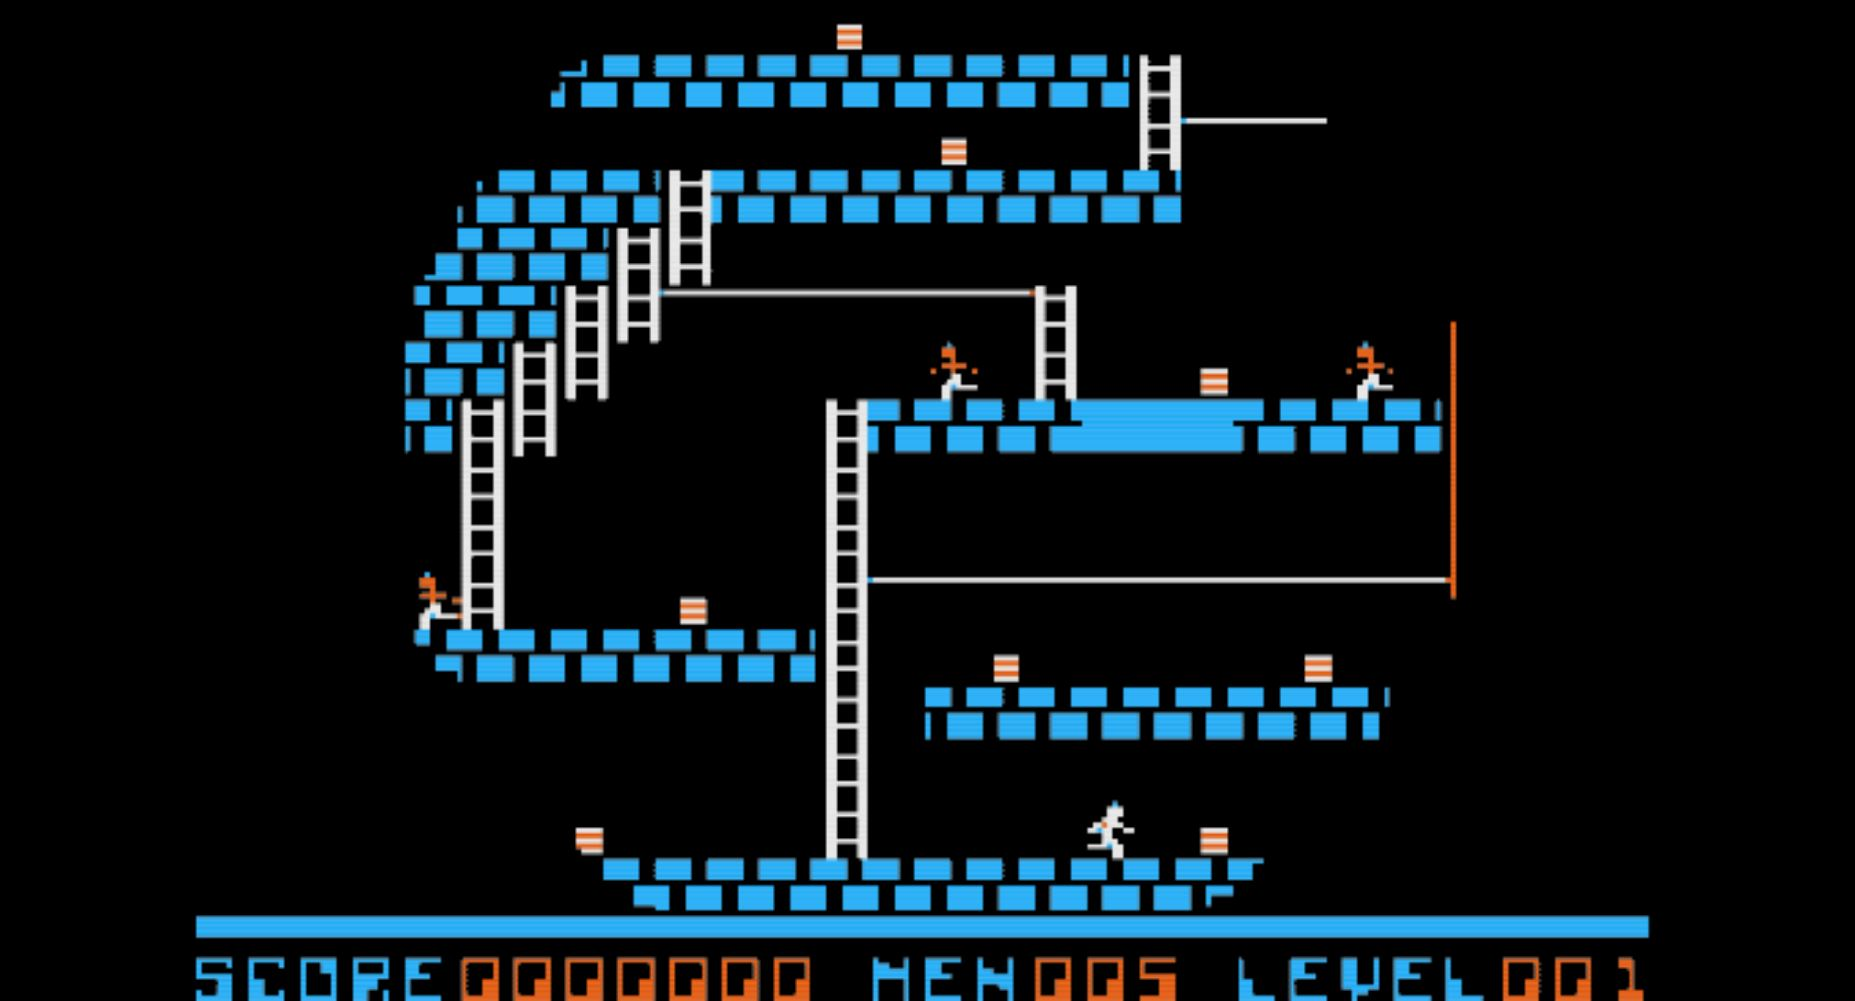
\includegraphics[width=\columnwidth]{iris}

\nwenddocs{}\nwbegincode{112}\sublabel{NW1Xx3lK-10jlgu-F}\nwmargintag{{\nwtagstyle{}\subpageref{NW1Xx3lK-10jlgu-F}}}\moddef{defines~{\nwtagstyle{}\subpageref{NW1Xx3lK-10jlgu-1}}}\plusendmoddef\nwstartdeflinemarkup\nwusesondefline{\\{NW1Xx3lK-1p0Y9w-1}}\nwprevnextdefs{NW1Xx3lK-10jlgu-E}{NW1Xx3lK-10jlgu-G}\nwenddeflinemarkup
\nwlinkedidentc{WIPE_COUNTER}{NW1Xx3lK-10jlgu-F}        EQU     $6D
\nwlinkedidentc{WIPE_MODE}{NW1Xx3lK-10jlgu-F}           EQU     $A5     ; 0 for open, 1 for close.
WIPE_DIR            EQU     $72     ; 0 for close, 1 for open.
WIPE_CENTER_X       EQU     $77
WIPE_CENTER_Y       EQU     $73
\nwindexdefn{\nwixident{WIPE{\_}COUNTER}}{WIPE:unCOUNTER}{NW1Xx3lK-10jlgu-F}\nwindexdefn{\nwixident{WIPE{\_}MODE}}{WIPE:unMODE}{NW1Xx3lK-10jlgu-F}\eatline
\nwused{\\{NW1Xx3lK-1p0Y9w-1}}\nwidentdefs{\\{{\nwixident{WIPE{\_}COUNTER}}{WIPE:unCOUNTER}}\\{{\nwixident{WIPE{\_}MODE}}{WIPE:unMODE}}}\nwendcode{}\nwbegindocs{113}\nwdocspar
\nwenddocs{}\nwbegincode{114}\sublabel{NW1Xx3lK-6p0m3-1}\nwmargintag{{\nwtagstyle{}\subpageref{NW1Xx3lK-6p0m3-1}}}\moddef{iris wipe~{\nwtagstyle{}\subpageref{NW1Xx3lK-6p0m3-1}}}\endmoddef\nwstartdeflinemarkup\nwusesondefline{\\{NW1Xx3lK-8jv1b-H}}\nwenddeflinemarkup
    ORG     $88A2
\nwlinkedidentc{IRIS_WIPE}{NW1Xx3lK-6p0m3-1}:
    SUBROUTINE

    LDA     88
    STA     WIPE_CENTER_Y
    LDA     140
    STA     WIPE_CENTER_X

    LDA     \nwlinkedidentc{WIPE_MODE}{NW1Xx3lK-10jlgu-F}
    BEQ     .iris_open

    LDX     #$AA
    STX     \nwlinkedidentc{WIPE_COUNTER}{NW1Xx3lK-10jlgu-F}
    LDX     #$00
    STX     WIPE_DIR             ; Close

.loop_close:
    JSR     \nwlinkedidentc{IRIS_WIPE_STEP}{NW1Xx3lK-1tGalf-1}
    DEC     \nwlinkedidentc{WIPE_COUNTER}{NW1Xx3lK-10jlgu-F}
    BNE     .loop_close

.iris_open:
    LDA     #$01
    STA     \nwlinkedidentc{WIPE_COUNTER}{NW1Xx3lK-10jlgu-F}
    STA     \nwlinkedidentc{WIPE_MODE}{NW1Xx3lK-10jlgu-F}           ; So next time we will close.
    STA     WIPE_DIR            ; Open
    JSR     \nwlinkedidentc{PUT_STATUS_LIVES}{NW1Xx3lK-8jv1b-E}
    JSR     \nwlinkedidentc{PUT_STATUS_LEVEL}{NW1Xx3lK-8jv1b-E}

.loop_open:
    JSR     \nwlinkedidentc{IRIS_WIPE_STEP}{NW1Xx3lK-1tGalf-1}
    INC     \nwlinkedidentc{WIPE_COUNTER}{NW1Xx3lK-10jlgu-F}
    LDA     \nwlinkedidentc{WIPE_COUNTER}{NW1Xx3lK-10jlgu-F}
    CMP     #$AA
    BNE     .loop_open
    RTS
\nwindexdefn{\nwixident{IRIS{\_}WIPE}}{IRIS:unWIPE}{NW1Xx3lK-6p0m3-1}\eatline
\nwused{\\{NW1Xx3lK-8jv1b-H}}\nwidentdefs{\\{{\nwixident{IRIS{\_}WIPE}}{IRIS:unWIPE}}}\nwidentuses{\\{{\nwixident{IRIS{\_}WIPE{\_}STEP}}{IRIS:unWIPE:unSTEP}}\\{{\nwixident{PUT{\_}STATUS{\_}LEVEL}}{PUT:unSTATUS:unLEVEL}}\\{{\nwixident{PUT{\_}STATUS{\_}LIVES}}{PUT:unSTATUS:unLIVES}}\\{{\nwixident{WIPE{\_}COUNTER}}{WIPE:unCOUNTER}}\\{{\nwixident{WIPE{\_}MODE}}{WIPE:unMODE}}}\nwindexuse{\nwixident{IRIS{\_}WIPE{\_}STEP}}{IRIS:unWIPE:unSTEP}{NW1Xx3lK-6p0m3-1}\nwindexuse{\nwixident{PUT{\_}STATUS{\_}LEVEL}}{PUT:unSTATUS:unLEVEL}{NW1Xx3lK-6p0m3-1}\nwindexuse{\nwixident{PUT{\_}STATUS{\_}LIVES}}{PUT:unSTATUS:unLIVES}{NW1Xx3lK-6p0m3-1}\nwindexuse{\nwixident{WIPE{\_}COUNTER}}{WIPE:unCOUNTER}{NW1Xx3lK-6p0m3-1}\nwindexuse{\nwixident{WIPE{\_}MODE}}{WIPE:unMODE}{NW1Xx3lK-6p0m3-1}\nwendcode{}\nwbegindocs{115}\nwdocspar
The routine {\Tt{}\nwlinkedidentq{IRIS{\_}WIPE{\_}STEP}{NW1Xx3lK-1tGalf-1}\nwendquote} does a lot of math to compute the circular iris, all parameterized
on {\Tt{}\nwlinkedidentq{WIPE{\_}COUNTER}{NW1Xx3lK-10jlgu-F}\nwendquote}.

Here is a routine that divides a 16-bit value in A and X (X being LSB) by 7, storing the
result in Y, with remainder in A. The routine effectively does long division. It also uses two temporaries.

\nwenddocs{}\nwbegincode{116}\sublabel{NW1Xx3lK-10jlgu-G}\nwmargintag{{\nwtagstyle{}\subpageref{NW1Xx3lK-10jlgu-G}}}\moddef{defines~{\nwtagstyle{}\subpageref{NW1Xx3lK-10jlgu-1}}}\plusendmoddef\nwstartdeflinemarkup\nwusesondefline{\\{NW1Xx3lK-1p0Y9w-1}}\nwprevnextdefs{NW1Xx3lK-10jlgu-F}{NW1Xx3lK-10jlgu-H}\nwenddeflinemarkup
\nwlinkedidentc{MATH_TMPL}{NW1Xx3lK-10jlgu-G}     EQU     $6F
\nwlinkedidentc{MATH_TMPH}{NW1Xx3lK-10jlgu-G}     EQU     $70
\nwindexdefn{\nwixident{MATH{\_}TMPL}}{MATH:unTMPL}{NW1Xx3lK-10jlgu-G}\nwindexdefn{\nwixident{MATH{\_}TMPH}}{MATH:unTMPH}{NW1Xx3lK-10jlgu-G}\eatline
\nwused{\\{NW1Xx3lK-1p0Y9w-1}}\nwidentdefs{\\{{\nwixident{MATH{\_}TMPH}}{MATH:unTMPH}}\\{{\nwixident{MATH{\_}TMPL}}{MATH:unTMPL}}}\nwendcode{}\nwbegindocs{117}\nwdocspar
\nwenddocs{}\nwbegincode{118}\sublabel{NW1Xx3lK-8jv1b-G}\nwmargintag{{\nwtagstyle{}\subpageref{NW1Xx3lK-8jv1b-G}}}\moddef{routines~{\nwtagstyle{}\subpageref{NW1Xx3lK-8jv1b-1}}}\plusendmoddef\nwstartdeflinemarkup\nwusesondefline{\\{NW1Xx3lK-1p0Y9w-1}}\nwprevnextdefs{NW1Xx3lK-8jv1b-F}{NW1Xx3lK-8jv1b-H}\nwenddeflinemarkup
    ORG     $8A45
\nwlinkedidentc{DIV_BY_7}{NW1Xx3lK-8jv1b-G}:
    SUBROUTINE
    ; Enter routine with AX set to (unsigned) numerator.
    ; On exit, Y will contain the integer portion of AX/7,
    ; and A contains the remainder.

    STX     \nwlinkedidentc{MATH_TMPL}{NW1Xx3lK-10jlgu-G}
    LDY     8
    SEC
    SBC     7

.loop:
    PHP
    ROL     \nwlinkedidentc{MATH_TMPH}{NW1Xx3lK-10jlgu-G}
    ASL     \nwlinkedidentc{MATH_TMPL}{NW1Xx3lK-10jlgu-G}
    ROL
    PLP
    BCC     .adjust_up
    SBC     7
    JMP     .next

.adjust_up
    ADC     7

.next
    DEY
    BNE     .loop

    BCS     .no_adjust
    ADC     7
    CLC

.no_adjust
    ROL     \nwlinkedidentc{MATH_TMPH}{NW1Xx3lK-10jlgu-G}
    LDY     \nwlinkedidentc{MATH_TMPH}{NW1Xx3lK-10jlgu-G}
    RTS
\nwindexdefn{\nwixident{DIV{\_}BY{\_}7}}{DIV:unBY:un7}{NW1Xx3lK-8jv1b-G}\eatline
\nwused{\\{NW1Xx3lK-1p0Y9w-1}}\nwidentdefs{\\{{\nwixident{DIV{\_}BY{\_}7}}{DIV:unBY:un7}}}\nwidentuses{\\{{\nwixident{MATH{\_}TMPH}}{MATH:unTMPH}}\\{{\nwixident{MATH{\_}TMPL}}{MATH:unTMPL}}}\nwindexuse{\nwixident{MATH{\_}TMPH}}{MATH:unTMPH}{NW1Xx3lK-8jv1b-G}\nwindexuse{\nwixident{MATH{\_}TMPL}}{MATH:unTMPL}{NW1Xx3lK-8jv1b-G}\nwendcode{}\nwbegindocs{119}\nwdocspar
Now, for one iris wipe step, we will need lots and lots of temporaries.

\nwenddocs{}\nwbegincode{120}\sublabel{NW1Xx3lK-10jlgu-H}\nwmargintag{{\nwtagstyle{}\subpageref{NW1Xx3lK-10jlgu-H}}}\moddef{defines~{\nwtagstyle{}\subpageref{NW1Xx3lK-10jlgu-1}}}\plusendmoddef\nwstartdeflinemarkup\nwusesondefline{\\{NW1Xx3lK-1p0Y9w-1}}\nwprevnextdefs{NW1Xx3lK-10jlgu-G}{\relax}\nwenddeflinemarkup
\nwlinkedidentc{WIPE0}{NW1Xx3lK-10jlgu-H}       EQU     $69     ; 16-bit value
\nwlinkedidentc{WIPE1}{NW1Xx3lK-10jlgu-H}       EQU     $67     ; 16-bit value
\nwlinkedidentc{WIPE2}{NW1Xx3lK-10jlgu-H}       EQU     $6B     ; 16-bit value
\nwlinkedidentc{WIPE3L}{NW1Xx3lK-10jlgu-H}      EQU     $75
\nwlinkedidentc{WIPE4L}{NW1Xx3lK-10jlgu-H}      EQU     $76
\nwlinkedidentc{WIPE5L}{NW1Xx3lK-10jlgu-H}      EQU     $77
\nwlinkedidentc{WIPE6L}{NW1Xx3lK-10jlgu-H}      EQU     $78
\nwlinkedidentc{WIPE3H}{NW1Xx3lK-10jlgu-H}      EQU     $79
\nwlinkedidentc{WIPE4H}{NW1Xx3lK-10jlgu-H}      EQU     $7A
\nwlinkedidentc{WIPE5H}{NW1Xx3lK-10jlgu-H}      EQU     $7B
\nwlinkedidentc{WIPE6H}{NW1Xx3lK-10jlgu-H}      EQU     $7C
\nwlinkedidentc{WIPE7D}{NW1Xx3lK-10jlgu-H}      EQU     $7D     ; Dividends
\nwlinkedidentc{WIPE8D}{NW1Xx3lK-10jlgu-H}      EQU     $7E
\nwlinkedidentc{WIPE9D}{NW1Xx3lK-10jlgu-H}      EQU     $7F
\nwlinkedidentc{WIPE10D}{NW1Xx3lK-10jlgu-H}     EQU     $80
\nwlinkedidentc{WIPE7R}{NW1Xx3lK-10jlgu-H}      EQU     $81     ; Remainders
\nwlinkedidentc{WIPE8R}{NW1Xx3lK-10jlgu-H}      EQU     $82
\nwlinkedidentc{WIPE9R}{NW1Xx3lK-10jlgu-H}      EQU     $83
\nwlinkedidentc{WIPE10R}{NW1Xx3lK-10jlgu-H}     EQU     $84
\nwindexdefn{\nwixident{WIPE0}}{WIPE0}{NW1Xx3lK-10jlgu-H}\nwindexdefn{\nwixident{WIPE1}}{WIPE1}{NW1Xx3lK-10jlgu-H}\nwindexdefn{\nwixident{WIPE2}}{WIPE2}{NW1Xx3lK-10jlgu-H}\nwindexdefn{\nwixident{WIPE3L}}{WIPE3L}{NW1Xx3lK-10jlgu-H}\nwindexdefn{\nwixident{WIPE3H}}{WIPE3H}{NW1Xx3lK-10jlgu-H}\nwindexdefn{\nwixident{WIPE4L}}{WIPE4L}{NW1Xx3lK-10jlgu-H}\nwindexdefn{\nwixident{WIPE4H}}{WIPE4H}{NW1Xx3lK-10jlgu-H}\nwindexdefn{\nwixident{WIPE5L}}{WIPE5L}{NW1Xx3lK-10jlgu-H}\nwindexdefn{\nwixident{WIPE5H}}{WIPE5H}{NW1Xx3lK-10jlgu-H}\nwindexdefn{\nwixident{WIPE6L}}{WIPE6L}{NW1Xx3lK-10jlgu-H}\nwindexdefn{\nwixident{WIPE6H}}{WIPE6H}{NW1Xx3lK-10jlgu-H}\nwindexdefn{\nwixident{WIPE7D}}{WIPE7D}{NW1Xx3lK-10jlgu-H}\nwindexdefn{\nwixident{WIPE7R}}{WIPE7R}{NW1Xx3lK-10jlgu-H}\nwindexdefn{\nwixident{WIPE8D}}{WIPE8D}{NW1Xx3lK-10jlgu-H}\nwindexdefn{\nwixident{WIPE8R}}{WIPE8R}{NW1Xx3lK-10jlgu-H}\nwindexdefn{\nwixident{WIPE9D}}{WIPE9D}{NW1Xx3lK-10jlgu-H}\nwindexdefn{\nwixident{WIPE9R}}{WIPE9R}{NW1Xx3lK-10jlgu-H}\nwindexdefn{\nwixident{WIPE10D}}{WIPE10D}{NW1Xx3lK-10jlgu-H}\nwindexdefn{\nwixident{WIPE10R}}{WIPE10R}{NW1Xx3lK-10jlgu-H}\eatline
\nwused{\\{NW1Xx3lK-1p0Y9w-1}}\nwidentdefs{\\{{\nwixident{WIPE0}}{WIPE0}}\\{{\nwixident{WIPE1}}{WIPE1}}\\{{\nwixident{WIPE10D}}{WIPE10D}}\\{{\nwixident{WIPE10R}}{WIPE10R}}\\{{\nwixident{WIPE2}}{WIPE2}}\\{{\nwixident{WIPE3H}}{WIPE3H}}\\{{\nwixident{WIPE3L}}{WIPE3L}}\\{{\nwixident{WIPE4H}}{WIPE4H}}\\{{\nwixident{WIPE4L}}{WIPE4L}}\\{{\nwixident{WIPE5H}}{WIPE5H}}\\{{\nwixident{WIPE5L}}{WIPE5L}}\\{{\nwixident{WIPE6H}}{WIPE6H}}\\{{\nwixident{WIPE6L}}{WIPE6L}}\\{{\nwixident{WIPE7D}}{WIPE7D}}\\{{\nwixident{WIPE7R}}{WIPE7R}}\\{{\nwixident{WIPE8D}}{WIPE8D}}\\{{\nwixident{WIPE8R}}{WIPE8R}}\\{{\nwixident{WIPE9D}}{WIPE9D}}\\{{\nwixident{WIPE9R}}{WIPE9R}}}\nwendcode{}\nwbegindocs{121}\nwdocspar
The first thing we do for a single step is initialize all those variables!

\nwenddocs{}\nwbegincode{122}\sublabel{NW1Xx3lK-1tGalf-1}\nwmargintag{{\nwtagstyle{}\subpageref{NW1Xx3lK-1tGalf-1}}}\moddef{iris wipe step~{\nwtagstyle{}\subpageref{NW1Xx3lK-1tGalf-1}}}\endmoddef\nwstartdeflinemarkup\nwusesondefline{\\{NW1Xx3lK-8jv1b-H}}\nwprevnextdefs{\relax}{NW1Xx3lK-1tGalf-2}\nwenddeflinemarkup
    ORG     $88D7
\nwlinkedidentc{IRIS_WIPE_STEP}{NW1Xx3lK-1tGalf-1}:
    SUBROUTINE

\LA{}\code{}WIPE0\ =\ WIPE{\_}COUNTER\edoc{}~{\nwtagstyle{}\subpageref{NW1Xx3lK-2Rx43B-1}}\RA{}
\LA{}\code{}WIPE1\ =\ 0\edoc{}~{\nwtagstyle{}\subpageref{NW1Xx3lK-1ZlBVV-1}}\RA{}
\LA{}\code{}WIPE2\ =\ 2\ *\ WIPE0\edoc{}~{\nwtagstyle{}\subpageref{NW1Xx3lK-39zOBY-1}}\RA{}
\LA{}\code{}WIPE2\ =\ 3\ -\ WIPE2\edoc{}~{\nwtagstyle{}\subpageref{NW1Xx3lK-1Ny5Ce-1}}\RA{}

; WIPE3, WIPE4, WIPE5, and WIPE6 correspond to
; row numbers. WIPE3 is above the center, WIPE6
; is below the center, while WIPE4 and WIPE5 are on
; the center.

\LA{}\code{}WIPE3\ =\ WIPE{\_}CENTER{\_}Y\ -\ WIPE{\_}COUNTER\edoc{}~{\nwtagstyle{}\subpageref{NW1Xx3lK-3R5hBF-1}}\RA{}
\LA{}\code{}WIPE4\ =\ WIPE5\ =\ WIPE{\_}CENTER{\_}Y\edoc{}~{\nwtagstyle{}\subpageref{NW1Xx3lK-2JOPWw-1}}\RA{}
\LA{}\code{}WIPE6\ =\ WIPE{\_}CENTER{\_}Y\ +\ WIPE{\_}COUNTER\edoc{}~{\nwtagstyle{}\subpageref{NW1Xx3lK-4TkslJ-1}}\RA{}

; WIPE7, WIPE8, WIPE9, and WIPE10 correspond to
; column byte numbers. Note the division by 7 pixels!
; WIPE7 is left of center, WIPE10 is right of center,
; while WIPE8 and WIPE9 are on the center.

\LA{}\code{}WIPE7\ =\ (WIPE{\_}CENTER{\_}X\ -\ WIPE{\_}COUNTER)\ /\ 7\edoc{}~{\nwtagstyle{}\subpageref{NW1Xx3lK-2ojStX-1}}\RA{}
\LA{}\code{}WIPE8\ =\ WIPE9\ =\ WIPE{\_}CENTER{\_}X\ /\ 7\edoc{}~{\nwtagstyle{}\subpageref{NW1Xx3lK-2QGdSi-1}}\RA{}
\LA{}\code{}WIPE10\ =\ (WIPE{\_}CENTER{\_}X\ +\ WIPE{\_}COUNTER)\ /\ 7\edoc{}~{\nwtagstyle{}\subpageref{NW1Xx3lK-2Um1dk-1}}\RA{}
\nwindexdefn{\nwixident{IRIS{\_}WIPE{\_}STEP}}{IRIS:unWIPE:unSTEP}{NW1Xx3lK-1tGalf-1}\eatline
\nwalsodefined{\\{NW1Xx3lK-1tGalf-2}}\nwused{\\{NW1Xx3lK-8jv1b-H}}\nwidentdefs{\\{{\nwixident{IRIS{\_}WIPE{\_}STEP}}{IRIS:unWIPE:unSTEP}}}\nwendcode{}\nwbegindocs{123}\nwdocspar
Now we loop. This involves checking {\Tt{}\nwlinkedidentq{WIPE1}{NW1Xx3lK-10jlgu-H}\nwendquote} against {\Tt{}\nwlinkedidentq{WIPE0}{NW1Xx3lK-10jlgu-H}\nwendquote}:

\begin{itemize}
  \item If {\Tt{}\nwlinkedidentq{WIPE1}{NW1Xx3lK-10jlgu-H}\nwendquote} $<$ {\Tt{}\nwlinkedidentq{WIPE0}{NW1Xx3lK-10jlgu-H}\nwendquote}, return.
  \item If {\Tt{}\nwlinkedidentq{WIPE1}{NW1Xx3lK-10jlgu-H}\nwendquote} == {\Tt{}\nwlinkedidentq{WIPE0}{NW1Xx3lK-10jlgu-H}\nwendquote}, go to {\Tt{}\nwlinkedidentq{DRAW{\_}WIPE{\_}STEP}{NW1Xx3lK-1DtO18-1}\nwendquote} then return.
  \item Otherwise, call {\Tt{}\nwlinkedidentq{DRAW{\_}WIPE{\_}STEP}{NW1Xx3lK-1DtO18-1}\nwendquote} and go round the loop.
\end{itemize}

Going around the loop involves calling {\Tt{}\nwlinkedidentq{DRAW{\_}WIPE{\_}STEP}{NW1Xx3lK-1DtO18-1}\nwendquote}, then adjusting
the numbers.

\nwenddocs{}\nwbegincode{124}\sublabel{NW1Xx3lK-1tGalf-2}\nwmargintag{{\nwtagstyle{}\subpageref{NW1Xx3lK-1tGalf-2}}}\moddef{iris wipe step~{\nwtagstyle{}\subpageref{NW1Xx3lK-1tGalf-1}}}\plusendmoddef\nwstartdeflinemarkup\nwusesondefline{\\{NW1Xx3lK-8jv1b-H}}\nwprevnextdefs{NW1Xx3lK-1tGalf-1}{\relax}\nwenddeflinemarkup
.loop:

\LA{}iris wipe loop check~{\nwtagstyle{}\subpageref{NW1Xx3lK-3vxyMm-1}}\RA{}

    JSR     \nwlinkedidentc{DRAW_WIPE_STEP}{NW1Xx3lK-1DtO18-1}

    LDA     \nwlinkedidentc{WIPE2}{NW1Xx3lK-10jlgu-H}+1
    BPL     .89a7

\LA{}\code{}WIPE2\ +=\ 4\ *\ WIPE1\ +\ 6\edoc{}~{\nwtagstyle{}\subpageref{NW1Xx3lK-mcL2B-1}}\RA{}
    JMP     .8a14

.89a7:

\LA{}\code{}WIPE2\ +=\ 4\ *\ (WIPE1\ -\ WIPE0)\ +\ 16\edoc{}~{\nwtagstyle{}\subpageref{NW1Xx3lK-2eL1Rw-1}}\RA{}
\LA{}Decrement \code{}WIPE0\edoc{}~{\nwtagstyle{}\subpageref{NW1Xx3lK-2u2rZr-1}}\RA{}
\LA{}Increment \code{}WIPE3\edoc{}~{\nwtagstyle{}\subpageref{NW1Xx3lK-13RMM3-1}}\RA{}
\LA{}Decrement \code{}WIPE10\edoc{} modulo 7~{\nwtagstyle{}\subpageref{NW1Xx3lK-11REH7-1}}\RA{}
\LA{}Increment \code{}WIPE7\edoc{} modulo 7~{\nwtagstyle{}\subpageref{NW1Xx3lK-11uG8h-1}}\RA{}
\LA{}Decrement \code{}WIPE6\edoc{}~{\nwtagstyle{}\subpageref{NW1Xx3lK-2u2n6B-1}}\RA{}

.8a14:

\LA{}Increment \code{}WIPE1\edoc{}~{\nwtagstyle{}\subpageref{NW1Xx3lK-13RECF-1}}\RA{}
\LA{}Increment \code{}WIPE9\edoc{} modulo 7~{\nwtagstyle{}\subpageref{NW1Xx3lK-3Y2gMs-1}}\RA{}
\LA{}Decrement \code{}WIPE4\edoc{}~{\nwtagstyle{}\subpageref{NW1Xx3lK-2u2srL-1}}\RA{}
\LA{}Increment \code{}WIPE5\edoc{}~{\nwtagstyle{}\subpageref{NW1Xx3lK-13RI6p-1}}\RA{}
\LA{}Decrement \code{}WIPE8\edoc{} modulo 7~{\nwtagstyle{}\subpageref{NW1Xx3lK-nzt1T-1}}\RA{}
    JMP     .loop
\nwused{\\{NW1Xx3lK-8jv1b-H}}\nwidentuses{\\{{\nwixident{DRAW{\_}WIPE{\_}STEP}}{DRAW:unWIPE:unSTEP}}\\{{\nwixident{WIPE2}}{WIPE2}}}\nwindexuse{\nwixident{DRAW{\_}WIPE{\_}STEP}}{DRAW:unWIPE:unSTEP}{NW1Xx3lK-1tGalf-2}\nwindexuse{\nwixident{WIPE2}}{WIPE2}{NW1Xx3lK-1tGalf-2}\nwendcode{}\nwbegindocs{125}\nwdocspar

Drawing a wipe step draws all four parts. There are two rows which move north
and two rows that move south. There are also two left and right offsets, one
short and one long. This makes eight combinations.

\nwenddocs{}\nwbegincode{126}\sublabel{NW1Xx3lK-1DtO18-1}\nwmargintag{{\nwtagstyle{}\subpageref{NW1Xx3lK-1DtO18-1}}}\moddef{draw wipe step~{\nwtagstyle{}\subpageref{NW1Xx3lK-1DtO18-1}}}\endmoddef\nwstartdeflinemarkup\nwusesondefline{\\{NW1Xx3lK-8jv1b-H}}\nwenddeflinemarkup
    ORG     $8A69
\nwlinkedidentc{DRAW_WIPE_STEP}{NW1Xx3lK-1DtO18-1}:
    SUBROUTINE

\LA{}Draw wipe for south part~{\nwtagstyle{}\subpageref{NW1Xx3lK-29jG99-1}}\RA{}
\LA{}Draw wipe for north part~{\nwtagstyle{}\subpageref{NW1Xx3lK-29yoMR-1}}\RA{}
\LA{}Draw wipe for north2 part~{\nwtagstyle{}\subpageref{NW1Xx3lK-3AjGdu-1}}\RA{}
\LA{}Draw wipe for south2 part~{\nwtagstyle{}\subpageref{NW1Xx3lK-3OCJye-1}}\RA{}
\nwindexdefn{\nwixident{DRAW{\_}WIPE{\_}STEP}}{DRAW:unWIPE:unSTEP}{NW1Xx3lK-1DtO18-1}\eatline
\nwused{\\{NW1Xx3lK-8jv1b-H}}\nwidentdefs{\\{{\nwixident{DRAW{\_}WIPE{\_}STEP}}{DRAW:unWIPE:unSTEP}}}\nwendcode{}\nwbegindocs{127}\nwdocspar
Each part consists of two halves, right and left (or east and west).

\nwenddocs{}\nwbegincode{128}\sublabel{NW1Xx3lK-29jG99-1}\nwmargintag{{\nwtagstyle{}\subpageref{NW1Xx3lK-29jG99-1}}}\moddef{Draw wipe for south part~{\nwtagstyle{}\subpageref{NW1Xx3lK-29jG99-1}}}\endmoddef\nwstartdeflinemarkup\nwusesondefline{\\{NW1Xx3lK-1DtO18-1}}\nwenddeflinemarkup
    LDY     \nwlinkedidentc{WIPE6H}{NW1Xx3lK-10jlgu-H}
    BNE     .draw_north
    LDY     \nwlinkedidentc{WIPE6L}{NW1Xx3lK-10jlgu-H}
    CPY     176
    BCS     .draw_north        ; Skip if WIPE6 >= 176

    JSR     \nwlinkedidentc{ROW_TO_ADDR_FOR_BOTH_PAGES}{NW1Xx3lK-8jv1b-4}

    ; East side
    LDY     \nwlinkedidentc{WIPE9D}{NW1Xx3lK-10jlgu-H}
    CPY     40
    BCS     .draw_south_west
    LDX     \nwlinkedidentc{WIPE9R}{NW1Xx3lK-10jlgu-H}
    JSR     \nwlinkedidentc{DRAW_WIPE_BLOCK}{NW1Xx3lK-32wUsj-1}

.draw_south_west
    ; West side
    LDY     \nwlinkedidentc{WIPE8D}{NW1Xx3lK-10jlgu-H}
    CPY     40
    BCS     .draw_north
    LDX     \nwlinkedidentc{WIPE9R}{NW1Xx3lK-10jlgu-H}
    JSR     \nwlinkedidentc{DRAW_WIPE_BLOCK}{NW1Xx3lK-32wUsj-1}
\nwused{\\{NW1Xx3lK-1DtO18-1}}\nwidentuses{\\{{\nwixident{DRAW{\_}WIPE{\_}BLOCK}}{DRAW:unWIPE:unBLOCK}}\\{{\nwixident{ROW{\_}TO{\_}ADDR{\_}FOR{\_}BOTH{\_}PAGES}}{ROW:unTO:unADDR:unFOR:unBOTH:unPAGES}}\\{{\nwixident{WIPE6H}}{WIPE6H}}\\{{\nwixident{WIPE6L}}{WIPE6L}}\\{{\nwixident{WIPE8D}}{WIPE8D}}\\{{\nwixident{WIPE9D}}{WIPE9D}}\\{{\nwixident{WIPE9R}}{WIPE9R}}}\nwindexuse{\nwixident{DRAW{\_}WIPE{\_}BLOCK}}{DRAW:unWIPE:unBLOCK}{NW1Xx3lK-29jG99-1}\nwindexuse{\nwixident{ROW{\_}TO{\_}ADDR{\_}FOR{\_}BOTH{\_}PAGES}}{ROW:unTO:unADDR:unFOR:unBOTH:unPAGES}{NW1Xx3lK-29jG99-1}\nwindexuse{\nwixident{WIPE6H}}{WIPE6H}{NW1Xx3lK-29jG99-1}\nwindexuse{\nwixident{WIPE6L}}{WIPE6L}{NW1Xx3lK-29jG99-1}\nwindexuse{\nwixident{WIPE8D}}{WIPE8D}{NW1Xx3lK-29jG99-1}\nwindexuse{\nwixident{WIPE9D}}{WIPE9D}{NW1Xx3lK-29jG99-1}\nwindexuse{\nwixident{WIPE9R}}{WIPE9R}{NW1Xx3lK-29jG99-1}\nwendcode{}\nwbegindocs{129}\nwdocspar

\nwenddocs{}\nwbegincode{130}\sublabel{NW1Xx3lK-29yoMR-1}\nwmargintag{{\nwtagstyle{}\subpageref{NW1Xx3lK-29yoMR-1}}}\moddef{Draw wipe for north part~{\nwtagstyle{}\subpageref{NW1Xx3lK-29yoMR-1}}}\endmoddef\nwstartdeflinemarkup\nwusesondefline{\\{NW1Xx3lK-1DtO18-1}}\nwenddeflinemarkup
.draw_north:
    LDY     \nwlinkedidentc{WIPE3H}{NW1Xx3lK-10jlgu-H}
    BNE     .draw_north2
    LDY     \nwlinkedidentc{WIPE3L}{NW1Xx3lK-10jlgu-H}
    CPY     176
    BCS     .draw_north2        ; Skip if WIPE3 >= 176

    JSR     \nwlinkedidentc{ROW_TO_ADDR_FOR_BOTH_PAGES}{NW1Xx3lK-8jv1b-4}

    ; East side
    LDY     \nwlinkedidentc{WIPE9D}{NW1Xx3lK-10jlgu-H}
    CPY     40
    BCS     .draw_north_west
    LDX     \nwlinkedidentc{WIPE9R}{NW1Xx3lK-10jlgu-H}
    JSR     \nwlinkedidentc{DRAW_WIPE_BLOCK}{NW1Xx3lK-32wUsj-1}

.draw_north_west
    ; West side
    LDY     \nwlinkedidentc{WIPE8D}{NW1Xx3lK-10jlgu-H}
    CPY     40
    BCS     .draw_north2
    LDX     \nwlinkedidentc{WIPE9R}{NW1Xx3lK-10jlgu-H}
    JSR     \nwlinkedidentc{DRAW_WIPE_BLOCK}{NW1Xx3lK-32wUsj-1}
\nwused{\\{NW1Xx3lK-1DtO18-1}}\nwidentuses{\\{{\nwixident{DRAW{\_}WIPE{\_}BLOCK}}{DRAW:unWIPE:unBLOCK}}\\{{\nwixident{ROW{\_}TO{\_}ADDR{\_}FOR{\_}BOTH{\_}PAGES}}{ROW:unTO:unADDR:unFOR:unBOTH:unPAGES}}\\{{\nwixident{WIPE3H}}{WIPE3H}}\\{{\nwixident{WIPE3L}}{WIPE3L}}\\{{\nwixident{WIPE8D}}{WIPE8D}}\\{{\nwixident{WIPE9D}}{WIPE9D}}\\{{\nwixident{WIPE9R}}{WIPE9R}}}\nwindexuse{\nwixident{DRAW{\_}WIPE{\_}BLOCK}}{DRAW:unWIPE:unBLOCK}{NW1Xx3lK-29yoMR-1}\nwindexuse{\nwixident{ROW{\_}TO{\_}ADDR{\_}FOR{\_}BOTH{\_}PAGES}}{ROW:unTO:unADDR:unFOR:unBOTH:unPAGES}{NW1Xx3lK-29yoMR-1}\nwindexuse{\nwixident{WIPE3H}}{WIPE3H}{NW1Xx3lK-29yoMR-1}\nwindexuse{\nwixident{WIPE3L}}{WIPE3L}{NW1Xx3lK-29yoMR-1}\nwindexuse{\nwixident{WIPE8D}}{WIPE8D}{NW1Xx3lK-29yoMR-1}\nwindexuse{\nwixident{WIPE9D}}{WIPE9D}{NW1Xx3lK-29yoMR-1}\nwindexuse{\nwixident{WIPE9R}}{WIPE9R}{NW1Xx3lK-29yoMR-1}\nwendcode{}\nwbegindocs{131}\nwdocspar

\nwenddocs{}\nwbegincode{132}\sublabel{NW1Xx3lK-3AjGdu-1}\nwmargintag{{\nwtagstyle{}\subpageref{NW1Xx3lK-3AjGdu-1}}}\moddef{Draw wipe for north2 part~{\nwtagstyle{}\subpageref{NW1Xx3lK-3AjGdu-1}}}\endmoddef\nwstartdeflinemarkup\nwusesondefline{\\{NW1Xx3lK-1DtO18-1}}\nwenddeflinemarkup
.draw_north2:
    LDY     \nwlinkedidentc{WIPE5H}{NW1Xx3lK-10jlgu-H}
    BNE     .draw_south2
    LDY     \nwlinkedidentc{WIPE5L}{NW1Xx3lK-10jlgu-H}
    CPY     176
    BCS     .draw_south2        ; Skip if WIPE5 >= 176

    JSR     \nwlinkedidentc{ROW_TO_ADDR_FOR_BOTH_PAGES}{NW1Xx3lK-8jv1b-4}

    ; East side
    LDY     \nwlinkedidentc{WIPE10D}{NW1Xx3lK-10jlgu-H}
    CPY     40
    BCS     .draw_north2_west
    LDX     \nwlinkedidentc{WIPE10R}{NW1Xx3lK-10jlgu-H}
    JSR     \nwlinkedidentc{DRAW_WIPE_BLOCK}{NW1Xx3lK-32wUsj-1}

.draw_north2_west
    ; West side
    LDY     \nwlinkedidentc{WIPE7D}{NW1Xx3lK-10jlgu-H}
    CPY     40
    BCS     .draw_south2
    LDX     \nwlinkedidentc{WIPE7R}{NW1Xx3lK-10jlgu-H}
    JSR     \nwlinkedidentc{DRAW_WIPE_BLOCK}{NW1Xx3lK-32wUsj-1}
\nwused{\\{NW1Xx3lK-1DtO18-1}}\nwidentuses{\\{{\nwixident{DRAW{\_}WIPE{\_}BLOCK}}{DRAW:unWIPE:unBLOCK}}\\{{\nwixident{ROW{\_}TO{\_}ADDR{\_}FOR{\_}BOTH{\_}PAGES}}{ROW:unTO:unADDR:unFOR:unBOTH:unPAGES}}\\{{\nwixident{WIPE10D}}{WIPE10D}}\\{{\nwixident{WIPE10R}}{WIPE10R}}\\{{\nwixident{WIPE5H}}{WIPE5H}}\\{{\nwixident{WIPE5L}}{WIPE5L}}\\{{\nwixident{WIPE7D}}{WIPE7D}}\\{{\nwixident{WIPE7R}}{WIPE7R}}}\nwindexuse{\nwixident{DRAW{\_}WIPE{\_}BLOCK}}{DRAW:unWIPE:unBLOCK}{NW1Xx3lK-3AjGdu-1}\nwindexuse{\nwixident{ROW{\_}TO{\_}ADDR{\_}FOR{\_}BOTH{\_}PAGES}}{ROW:unTO:unADDR:unFOR:unBOTH:unPAGES}{NW1Xx3lK-3AjGdu-1}\nwindexuse{\nwixident{WIPE10D}}{WIPE10D}{NW1Xx3lK-3AjGdu-1}\nwindexuse{\nwixident{WIPE10R}}{WIPE10R}{NW1Xx3lK-3AjGdu-1}\nwindexuse{\nwixident{WIPE5H}}{WIPE5H}{NW1Xx3lK-3AjGdu-1}\nwindexuse{\nwixident{WIPE5L}}{WIPE5L}{NW1Xx3lK-3AjGdu-1}\nwindexuse{\nwixident{WIPE7D}}{WIPE7D}{NW1Xx3lK-3AjGdu-1}\nwindexuse{\nwixident{WIPE7R}}{WIPE7R}{NW1Xx3lK-3AjGdu-1}\nwendcode{}\nwbegindocs{133}\nwdocspar

\nwenddocs{}\nwbegincode{134}\sublabel{NW1Xx3lK-3OCJye-1}\nwmargintag{{\nwtagstyle{}\subpageref{NW1Xx3lK-3OCJye-1}}}\moddef{Draw wipe for south2 part~{\nwtagstyle{}\subpageref{NW1Xx3lK-3OCJye-1}}}\endmoddef\nwstartdeflinemarkup\nwusesondefline{\\{NW1Xx3lK-1DtO18-1}}\nwenddeflinemarkup
.draw_south2:
    LDY     \nwlinkedidentc{WIPE4H}{NW1Xx3lK-10jlgu-H}
    BNE     .end
    LDY     \nwlinkedidentc{WIPE4L}{NW1Xx3lK-10jlgu-H}
    CPY     176
    BCS     .end        ; Skip if WIPE4 >= 176

    JSR     \nwlinkedidentc{ROW_TO_ADDR_FOR_BOTH_PAGES}{NW1Xx3lK-8jv1b-4}

    ; East side
    LDY     \nwlinkedidentc{WIPE10D}{NW1Xx3lK-10jlgu-H}
    CPY     40
    BCS     .draw_south2_west
    LDX     \nwlinkedidentc{WIPE10R}{NW1Xx3lK-10jlgu-H}
    JSR     \nwlinkedidentc{DRAW_WIPE_BLOCK}{NW1Xx3lK-32wUsj-1}

.draw_south2_west
    ; West side
    LDY     \nwlinkedidentc{WIPE7D}{NW1Xx3lK-10jlgu-H}
    CPY     40
    BCS     .draw_south2
    LDX     \nwlinkedidentc{WIPE7R}{NW1Xx3lK-10jlgu-H}
    JMP     \nwlinkedidentc{DRAW_WIPE_BLOCK}{NW1Xx3lK-32wUsj-1}           ; tail call

.end:
    RTS
\nwused{\\{NW1Xx3lK-1DtO18-1}}\nwidentuses{\\{{\nwixident{DRAW{\_}WIPE{\_}BLOCK}}{DRAW:unWIPE:unBLOCK}}\\{{\nwixident{ROW{\_}TO{\_}ADDR{\_}FOR{\_}BOTH{\_}PAGES}}{ROW:unTO:unADDR:unFOR:unBOTH:unPAGES}}\\{{\nwixident{WIPE10D}}{WIPE10D}}\\{{\nwixident{WIPE10R}}{WIPE10R}}\\{{\nwixident{WIPE4H}}{WIPE4H}}\\{{\nwixident{WIPE4L}}{WIPE4L}}\\{{\nwixident{WIPE7D}}{WIPE7D}}\\{{\nwixident{WIPE7R}}{WIPE7R}}}\nwindexuse{\nwixident{DRAW{\_}WIPE{\_}BLOCK}}{DRAW:unWIPE:unBLOCK}{NW1Xx3lK-3OCJye-1}\nwindexuse{\nwixident{ROW{\_}TO{\_}ADDR{\_}FOR{\_}BOTH{\_}PAGES}}{ROW:unTO:unADDR:unFOR:unBOTH:unPAGES}{NW1Xx3lK-3OCJye-1}\nwindexuse{\nwixident{WIPE10D}}{WIPE10D}{NW1Xx3lK-3OCJye-1}\nwindexuse{\nwixident{WIPE10R}}{WIPE10R}{NW1Xx3lK-3OCJye-1}\nwindexuse{\nwixident{WIPE4H}}{WIPE4H}{NW1Xx3lK-3OCJye-1}\nwindexuse{\nwixident{WIPE4L}}{WIPE4L}{NW1Xx3lK-3OCJye-1}\nwindexuse{\nwixident{WIPE7D}}{WIPE7D}{NW1Xx3lK-3OCJye-1}\nwindexuse{\nwixident{WIPE7R}}{WIPE7R}{NW1Xx3lK-3OCJye-1}\nwendcode{}\nwbegindocs{135}\nwdocspar

Drawing a wipe block depends on whether we're opening or closing on the level.
Closing on the level just blacks out pixels on page 1. Opening on the level
copies some pixels from page 2 into page 1.

\nwenddocs{}\nwbegincode{136}\sublabel{NW1Xx3lK-32wUsj-1}\nwmargintag{{\nwtagstyle{}\subpageref{NW1Xx3lK-32wUsj-1}}}\moddef{draw wipe block~{\nwtagstyle{}\subpageref{NW1Xx3lK-32wUsj-1}}}\endmoddef\nwstartdeflinemarkup\nwusesondefline{\\{NW1Xx3lK-8jv1b-H}}\nwenddeflinemarkup
    ORG     $8AF6
\nwlinkedidentc{DRAW_WIPE_BLOCK}{NW1Xx3lK-32wUsj-1}:
    SUBROUTINE
    ; Enter routine with X set to the column byte and Y set to
    ; the pixel number within that byte (0-6). \nwlinkedidentc{ROW_ADDR}{NW1Xx3lK-10jlgu-4} and
    ; \nwlinkedidentc{ROW_ADDR2}{NW1Xx3lK-10jlgu-4} must contain the base row address for page 1
    ; and page 2, respectively.

    LDA     WIPE_DIR
    BNE     .open
    LDA     (\nwlinkedidentc{ROW_ADDR}{NW1Xx3lK-10jlgu-4}),Y
    AND     \nwlinkedidentc{WIPE_BLOCK_CLOSE_MASK}{NW1Xx3lK-1W8AJS-B},X
    STA     (\nwlinkedidentc{ROW_ADDR}{NW1Xx3lK-10jlgu-4}),Y

.open:
    LDA     (\nwlinkedidentc{ROW_ADDR2}{NW1Xx3lK-10jlgu-4}),Y
    AND     \nwlinkedidentc{WIPE_BLOCK_OPEN_MASK}{NW1Xx3lK-1W8AJS-B},X
    ORA     (\nwlinkedidentc{ROW_ADDR}{NW1Xx3lK-10jlgu-4}),Y
    STA     (\nwlinkedidentc{ROW_ADDR}{NW1Xx3lK-10jlgu-4}),Y
    RTS
\nwindexdefn{\nwixident{DRAW{\_}WIPE{\_}BLOCK}}{DRAW:unWIPE:unBLOCK}{NW1Xx3lK-32wUsj-1}\eatline
\nwused{\\{NW1Xx3lK-8jv1b-H}}\nwidentdefs{\\{{\nwixident{DRAW{\_}WIPE{\_}BLOCK}}{DRAW:unWIPE:unBLOCK}}}\nwidentuses{\\{{\nwixident{ROW{\_}ADDR}}{ROW:unADDR}}\\{{\nwixident{ROW{\_}ADDR2}}{ROW:unADDR2}}\\{{\nwixident{WIPE{\_}BLOCK{\_}CLOSE{\_}MASK}}{WIPE:unBLOCK:unCLOSE:unMASK}}\\{{\nwixident{WIPE{\_}BLOCK{\_}OPEN{\_}MASK}}{WIPE:unBLOCK:unOPEN:unMASK}}}\nwindexuse{\nwixident{ROW{\_}ADDR}}{ROW:unADDR}{NW1Xx3lK-32wUsj-1}\nwindexuse{\nwixident{ROW{\_}ADDR2}}{ROW:unADDR2}{NW1Xx3lK-32wUsj-1}\nwindexuse{\nwixident{WIPE{\_}BLOCK{\_}CLOSE{\_}MASK}}{WIPE:unBLOCK:unCLOSE:unMASK}{NW1Xx3lK-32wUsj-1}\nwindexuse{\nwixident{WIPE{\_}BLOCK{\_}OPEN{\_}MASK}}{WIPE:unBLOCK:unOPEN:unMASK}{NW1Xx3lK-32wUsj-1}\nwendcode{}\nwbegindocs{137}\nwdocspar
\nwenddocs{}\nwbegincode{138}\sublabel{NW1Xx3lK-1W8AJS-B}\nwmargintag{{\nwtagstyle{}\subpageref{NW1Xx3lK-1W8AJS-B}}}\moddef{tables~{\nwtagstyle{}\subpageref{NW1Xx3lK-1W8AJS-1}}}\plusendmoddef\nwstartdeflinemarkup\nwusesondefline{\\{NW1Xx3lK-1p0Y9w-1}}\nwprevnextdefs{NW1Xx3lK-1W8AJS-A}{\relax}\nwenddeflinemarkup
    ORG     $8B0C
\nwlinkedidentc{WIPE_BLOCK_CLOSE_MASK}{NW1Xx3lK-1W8AJS-B}:
    BYTE     %11110000
    BYTE     %11110000
    BYTE     %11110000
    BYTE     %11110000
    BYTE     %10001111
    BYTE     %10001111
    BYTE     %10001111
\nwlinkedidentc{WIPE_BLOCK_OPEN_MASK}{NW1Xx3lK-1W8AJS-B}:
    BYTE     %10001111
    BYTE     %10001111
    BYTE     %10001111
    BYTE     %10001111
    BYTE     %11110000
    BYTE     %11110000
    BYTE     %11110000
\nwindexdefn{\nwixident{WIPE{\_}BLOCK{\_}CLOSE{\_}MASK}}{WIPE:unBLOCK:unCLOSE:unMASK}{NW1Xx3lK-1W8AJS-B}\nwindexdefn{\nwixident{WIPE{\_}BLOCK{\_}OPEN{\_}MASK}}{WIPE:unBLOCK:unOPEN:unMASK}{NW1Xx3lK-1W8AJS-B}\eatline
\nwused{\\{NW1Xx3lK-1p0Y9w-1}}\nwidentdefs{\\{{\nwixident{WIPE{\_}BLOCK{\_}CLOSE{\_}MASK}}{WIPE:unBLOCK:unCLOSE:unMASK}}\\{{\nwixident{WIPE{\_}BLOCK{\_}OPEN{\_}MASK}}{WIPE:unBLOCK:unOPEN:unMASK}}}\nwendcode{}\nwbegindocs{139}\nwdocspar
\nwenddocs{}\nwbegincode{140}\sublabel{NW1Xx3lK-3vxyMm-1}\nwmargintag{{\nwtagstyle{}\subpageref{NW1Xx3lK-3vxyMm-1}}}\moddef{iris wipe loop check~{\nwtagstyle{}\subpageref{NW1Xx3lK-3vxyMm-1}}}\endmoddef\nwstartdeflinemarkup\nwusesondefline{\\{NW1Xx3lK-1tGalf-2}}\nwenddeflinemarkup
    LDA     \nwlinkedidentc{WIPE1}{NW1Xx3lK-10jlgu-H}+1
    CMP     \nwlinkedidentc{WIPE0}{NW1Xx3lK-10jlgu-H}+1
    BCC     .draw_wipe_step ; Effectively, if \nwlinkedidentc{WIPE1}{NW1Xx3lK-10jlgu-H} > \nwlinkedidentc{WIPE0}{NW1Xx3lK-10jlgu-H}, jump to .draw_wipe_step.
    BEQ     .8969           ; Otherwise jump to .loop1, which...

.loop1:
    LDA     \nwlinkedidentc{WIPE1}{NW1Xx3lK-10jlgu-H}
    CMP     \nwlinkedidentc{WIPE0}{NW1Xx3lK-10jlgu-H}
    BNE     .end
    LDA     \nwlinkedidentc{WIPE1}{NW1Xx3lK-10jlgu-H}+1
    CMP     \nwlinkedidentc{WIPE0}{NW1Xx3lK-10jlgu-H}+1
    BNE     .end            ; If \nwlinkedidentc{WIPE0}{NW1Xx3lK-10jlgu-H} != \nwlinkedidentc{WIPE1}{NW1Xx3lK-10jlgu-H}, return.
    JMP     \nwlinkedidentc{DRAW_WIPE_STEP}{NW1Xx3lK-1DtO18-1}

.end:
    RTS

.8969:
    LDA     \nwlinkedidentc{WIPE1}{NW1Xx3lK-10jlgu-H}
    CMP     \nwlinkedidentc{WIPE0}{NW1Xx3lK-10jlgu-H}
    BCS     .loop1          ; The other half of the comparison from .loop.

.draw_wipe_step:
\nwused{\\{NW1Xx3lK-1tGalf-2}}\nwidentuses{\\{{\nwixident{DRAW{\_}WIPE{\_}STEP}}{DRAW:unWIPE:unSTEP}}\\{{\nwixident{WIPE0}}{WIPE0}}\\{{\nwixident{WIPE1}}{WIPE1}}}\nwindexuse{\nwixident{DRAW{\_}WIPE{\_}STEP}}{DRAW:unWIPE:unSTEP}{NW1Xx3lK-3vxyMm-1}\nwindexuse{\nwixident{WIPE0}}{WIPE0}{NW1Xx3lK-3vxyMm-1}\nwindexuse{\nwixident{WIPE1}}{WIPE1}{NW1Xx3lK-3vxyMm-1}\nwendcode{}\nwbegindocs{141}\nwdocspar

\subsection{Initialization}

\nwenddocs{}\nwbegincode{142}\sublabel{NW1Xx3lK-2Rx43B-1}\nwmargintag{{\nwtagstyle{}\subpageref{NW1Xx3lK-2Rx43B-1}}}\moddef{\code{}WIPE0\ =\ WIPE{\_}COUNTER\edoc{}~{\nwtagstyle{}\subpageref{NW1Xx3lK-2Rx43B-1}}}\endmoddef\nwstartdeflinemarkup\nwusesondefline{\\{NW1Xx3lK-1tGalf-1}}\nwenddeflinemarkup
    LDA     \nwlinkedidentc{WIPE_COUNTER}{NW1Xx3lK-10jlgu-F}
    STA     \nwlinkedidentc{WIPE0}{NW1Xx3lK-10jlgu-H}
    LDA     #$00
    STA     \nwlinkedidentc{WIPE0}{NW1Xx3lK-10jlgu-H}+1         ; \nwlinkedidentc{WIPE0}{NW1Xx3lK-10jlgu-H} = \nwlinkedidentc{WIPE_COUNTER}{NW1Xx3lK-10jlgu-F}
\nwused{\\{NW1Xx3lK-1tGalf-1}}\nwidentuses{\\{{\nwixident{WIPE0}}{WIPE0}}\\{{\nwixident{WIPE{\_}COUNTER}}{WIPE:unCOUNTER}}}\nwindexuse{\nwixident{WIPE0}}{WIPE0}{NW1Xx3lK-2Rx43B-1}\nwindexuse{\nwixident{WIPE{\_}COUNTER}}{WIPE:unCOUNTER}{NW1Xx3lK-2Rx43B-1}\nwendcode{}\nwbegindocs{143}\nwdocspar

\nwenddocs{}\nwbegincode{144}\sublabel{NW1Xx3lK-1ZlBVV-1}\nwmargintag{{\nwtagstyle{}\subpageref{NW1Xx3lK-1ZlBVV-1}}}\moddef{\code{}WIPE1\ =\ 0\edoc{}~{\nwtagstyle{}\subpageref{NW1Xx3lK-1ZlBVV-1}}}\endmoddef\nwstartdeflinemarkup\nwusesondefline{\\{NW1Xx3lK-1tGalf-1}}\nwenddeflinemarkup
    ; fallthrough with A = 0
    STA     \nwlinkedidentc{WIPE1}{NW1Xx3lK-10jlgu-H}
    STA     \nwlinkedidentc{WIPE1}{NW1Xx3lK-10jlgu-H}+1         ; \nwlinkedidentc{WIPE1}{NW1Xx3lK-10jlgu-H} = 0
\nwused{\\{NW1Xx3lK-1tGalf-1}}\nwidentuses{\\{{\nwixident{WIPE1}}{WIPE1}}}\nwindexuse{\nwixident{WIPE1}}{WIPE1}{NW1Xx3lK-1ZlBVV-1}\nwendcode{}\nwbegindocs{145}\nwdocspar

\nwenddocs{}\nwbegincode{146}\sublabel{NW1Xx3lK-39zOBY-1}\nwmargintag{{\nwtagstyle{}\subpageref{NW1Xx3lK-39zOBY-1}}}\moddef{\code{}WIPE2\ =\ 2\ *\ WIPE0\edoc{}~{\nwtagstyle{}\subpageref{NW1Xx3lK-39zOBY-1}}}\endmoddef\nwstartdeflinemarkup\nwusesondefline{\\{NW1Xx3lK-1tGalf-1}}\nwenddeflinemarkup
    LDA     \nwlinkedidentc{WIPE0}{NW1Xx3lK-10jlgu-H}
    ASL
    STA     \nwlinkedidentc{WIPE2}{NW1Xx3lK-10jlgu-H}
    LDA     \nwlinkedidentc{WIPE0}{NW1Xx3lK-10jlgu-H}+1
    ROL
    STA     \nwlinkedidentc{WIPE2}{NW1Xx3lK-10jlgu-H}+1         ; \nwlinkedidentc{WIPE2}{NW1Xx3lK-10jlgu-H} = 2 * \nwlinkedidentc{WIPE0}{NW1Xx3lK-10jlgu-H}
\nwused{\\{NW1Xx3lK-1tGalf-1}}\nwidentuses{\\{{\nwixident{WIPE0}}{WIPE0}}\\{{\nwixident{WIPE2}}{WIPE2}}}\nwindexuse{\nwixident{WIPE0}}{WIPE0}{NW1Xx3lK-39zOBY-1}\nwindexuse{\nwixident{WIPE2}}{WIPE2}{NW1Xx3lK-39zOBY-1}\nwendcode{}\nwbegindocs{147}\nwdocspar

\nwenddocs{}\nwbegincode{148}\sublabel{NW1Xx3lK-1Ny5Ce-1}\nwmargintag{{\nwtagstyle{}\subpageref{NW1Xx3lK-1Ny5Ce-1}}}\moddef{\code{}WIPE2\ =\ 3\ -\ WIPE2\edoc{}~{\nwtagstyle{}\subpageref{NW1Xx3lK-1Ny5Ce-1}}}\endmoddef\nwstartdeflinemarkup\nwusesondefline{\\{NW1Xx3lK-1tGalf-1}}\nwenddeflinemarkup
    LDA     #$03
    SEC
    SBC     \nwlinkedidentc{WIPE2}{NW1Xx3lK-10jlgu-H}
    STA     \nwlinkedidentc{WIPE2}{NW1Xx3lK-10jlgu-H}
    LDA     #$00
    SBC     \nwlinkedidentc{WIPE2}{NW1Xx3lK-10jlgu-H}+1
    STA     \nwlinkedidentc{WIPE2}{NW1Xx3lK-10jlgu-H}+1         ; \nwlinkedidentc{WIPE2}{NW1Xx3lK-10jlgu-H} = 3 - \nwlinkedidentc{WIPE2}{NW1Xx3lK-10jlgu-H}
\nwused{\\{NW1Xx3lK-1tGalf-1}}\nwidentuses{\\{{\nwixident{WIPE2}}{WIPE2}}}\nwindexuse{\nwixident{WIPE2}}{WIPE2}{NW1Xx3lK-1Ny5Ce-1}\nwendcode{}\nwbegindocs{149}\nwdocspar

\nwenddocs{}\nwbegincode{150}\sublabel{NW1Xx3lK-3R5hBF-1}\nwmargintag{{\nwtagstyle{}\subpageref{NW1Xx3lK-3R5hBF-1}}}\moddef{\code{}WIPE3\ =\ WIPE{\_}CENTER{\_}Y\ -\ WIPE{\_}COUNTER\edoc{}~{\nwtagstyle{}\subpageref{NW1Xx3lK-3R5hBF-1}}}\endmoddef\nwstartdeflinemarkup\nwusesondefline{\\{NW1Xx3lK-1tGalf-1}}\nwenddeflinemarkup
    LDA     WIPE_CENTER_Y
    SEC
    SBC     \nwlinkedidentc{WIPE_COUNTER}{NW1Xx3lK-10jlgu-F}
    STA     \nwlinkedidentc{WIPE3L}{NW1Xx3lK-10jlgu-H}
    LDA     #$00
    SBC     #$00
    STA     \nwlinkedidentc{WIPE3H}{NW1Xx3lK-10jlgu-H}          ; WIPE3 = WIPE_CENTER_Y - \nwlinkedidentc{WIPE_COUNTER}{NW1Xx3lK-10jlgu-F}
\nwused{\\{NW1Xx3lK-1tGalf-1}}\nwidentuses{\\{{\nwixident{WIPE3H}}{WIPE3H}}\\{{\nwixident{WIPE3L}}{WIPE3L}}\\{{\nwixident{WIPE{\_}COUNTER}}{WIPE:unCOUNTER}}}\nwindexuse{\nwixident{WIPE3H}}{WIPE3H}{NW1Xx3lK-3R5hBF-1}\nwindexuse{\nwixident{WIPE3L}}{WIPE3L}{NW1Xx3lK-3R5hBF-1}\nwindexuse{\nwixident{WIPE{\_}COUNTER}}{WIPE:unCOUNTER}{NW1Xx3lK-3R5hBF-1}\nwendcode{}\nwbegindocs{151}\nwdocspar

\nwenddocs{}\nwbegincode{152}\sublabel{NW1Xx3lK-2JOPWw-1}\nwmargintag{{\nwtagstyle{}\subpageref{NW1Xx3lK-2JOPWw-1}}}\moddef{\code{}WIPE4\ =\ WIPE5\ =\ WIPE{\_}CENTER{\_}Y\edoc{}~{\nwtagstyle{}\subpageref{NW1Xx3lK-2JOPWw-1}}}\endmoddef\nwstartdeflinemarkup\nwusesondefline{\\{NW1Xx3lK-1tGalf-1}}\nwenddeflinemarkup
    LDA     WIPE_CENTER_Y
    STA     \nwlinkedidentc{WIPE4L}{NW1Xx3lK-10jlgu-H}
    STA     \nwlinkedidentc{WIPE5L}{NW1Xx3lK-10jlgu-H}
    LDA     #$00
    STA     \nwlinkedidentc{WIPE4H}{NW1Xx3lK-10jlgu-H}
    STA     \nwlinkedidentc{WIPE5H}{NW1Xx3lK-10jlgu-H}          ; WIPE4 = WIPE5 = WIPE_CENTER_Y
\nwused{\\{NW1Xx3lK-1tGalf-1}}\nwidentuses{\\{{\nwixident{WIPE4H}}{WIPE4H}}\\{{\nwixident{WIPE4L}}{WIPE4L}}\\{{\nwixident{WIPE5H}}{WIPE5H}}\\{{\nwixident{WIPE5L}}{WIPE5L}}}\nwindexuse{\nwixident{WIPE4H}}{WIPE4H}{NW1Xx3lK-2JOPWw-1}\nwindexuse{\nwixident{WIPE4L}}{WIPE4L}{NW1Xx3lK-2JOPWw-1}\nwindexuse{\nwixident{WIPE5H}}{WIPE5H}{NW1Xx3lK-2JOPWw-1}\nwindexuse{\nwixident{WIPE5L}}{WIPE5L}{NW1Xx3lK-2JOPWw-1}\nwendcode{}\nwbegindocs{153}\nwdocspar

\nwenddocs{}\nwbegincode{154}\sublabel{NW1Xx3lK-4TkslJ-1}\nwmargintag{{\nwtagstyle{}\subpageref{NW1Xx3lK-4TkslJ-1}}}\moddef{\code{}WIPE6\ =\ WIPE{\_}CENTER{\_}Y\ +\ WIPE{\_}COUNTER\edoc{}~{\nwtagstyle{}\subpageref{NW1Xx3lK-4TkslJ-1}}}\endmoddef\nwstartdeflinemarkup\nwusesondefline{\\{NW1Xx3lK-1tGalf-1}}\nwenddeflinemarkup
    LDA     WIPE_CENTER_Y
    CLC
    ADC     \nwlinkedidentc{WIPE_COUNTER}{NW1Xx3lK-10jlgu-F}
    STA     \nwlinkedidentc{WIPE6L}{NW1Xx3lK-10jlgu-H}
    LDA     #$00
    ADC     #$00
    STA     \nwlinkedidentc{WIPE6H}{NW1Xx3lK-10jlgu-H}          ; WIPE6 = WIPE_CENTER_Y + \nwlinkedidentc{WIPE_COUNTER}{NW1Xx3lK-10jlgu-F}
\nwused{\\{NW1Xx3lK-1tGalf-1}}\nwidentuses{\\{{\nwixident{WIPE6H}}{WIPE6H}}\\{{\nwixident{WIPE6L}}{WIPE6L}}\\{{\nwixident{WIPE{\_}COUNTER}}{WIPE:unCOUNTER}}}\nwindexuse{\nwixident{WIPE6H}}{WIPE6H}{NW1Xx3lK-4TkslJ-1}\nwindexuse{\nwixident{WIPE6L}}{WIPE6L}{NW1Xx3lK-4TkslJ-1}\nwindexuse{\nwixident{WIPE{\_}COUNTER}}{WIPE:unCOUNTER}{NW1Xx3lK-4TkslJ-1}\nwendcode{}\nwbegindocs{155}\nwdocspar

\nwenddocs{}\nwbegincode{156}\sublabel{NW1Xx3lK-2ojStX-1}\nwmargintag{{\nwtagstyle{}\subpageref{NW1Xx3lK-2ojStX-1}}}\moddef{\code{}WIPE7\ =\ (WIPE{\_}CENTER{\_}X\ -\ WIPE{\_}COUNTER)\ /\ 7\edoc{}~{\nwtagstyle{}\subpageref{NW1Xx3lK-2ojStX-1}}}\endmoddef\nwstartdeflinemarkup\nwusesondefline{\\{NW1Xx3lK-1tGalf-1}}\nwenddeflinemarkup
    LDA     WIPE_CENTER_X
    SEC
    SBC     \nwlinkedidentc{WIPE_COUNTER}{NW1Xx3lK-10jlgu-F}
    TAX
    LDA     #$00
    SBC     #$00
    JSR     \nwlinkedidentc{DIV_BY_7}{NW1Xx3lK-8jv1b-G}
    STY     \nwlinkedidentc{WIPE7D}{NW1Xx3lK-10jlgu-H}
    STA     \nwlinkedidentc{WIPE7R}{NW1Xx3lK-10jlgu-H}          ; WIPE7 = (WIPE_CENTER_X - \nwlinkedidentc{WIPE_COUNTER}{NW1Xx3lK-10jlgu-F}) / 7
\nwused{\\{NW1Xx3lK-1tGalf-1}}\nwidentuses{\\{{\nwixident{DIV{\_}BY{\_}7}}{DIV:unBY:un7}}\\{{\nwixident{WIPE7D}}{WIPE7D}}\\{{\nwixident{WIPE7R}}{WIPE7R}}\\{{\nwixident{WIPE{\_}COUNTER}}{WIPE:unCOUNTER}}}\nwindexuse{\nwixident{DIV{\_}BY{\_}7}}{DIV:unBY:un7}{NW1Xx3lK-2ojStX-1}\nwindexuse{\nwixident{WIPE7D}}{WIPE7D}{NW1Xx3lK-2ojStX-1}\nwindexuse{\nwixident{WIPE7R}}{WIPE7R}{NW1Xx3lK-2ojStX-1}\nwindexuse{\nwixident{WIPE{\_}COUNTER}}{WIPE:unCOUNTER}{NW1Xx3lK-2ojStX-1}\nwendcode{}\nwbegindocs{157}\nwdocspar

\nwenddocs{}\nwbegincode{158}\sublabel{NW1Xx3lK-2QGdSi-1}\nwmargintag{{\nwtagstyle{}\subpageref{NW1Xx3lK-2QGdSi-1}}}\moddef{\code{}WIPE8\ =\ WIPE9\ =\ WIPE{\_}CENTER{\_}X\ /\ 7\edoc{}~{\nwtagstyle{}\subpageref{NW1Xx3lK-2QGdSi-1}}}\endmoddef\nwstartdeflinemarkup\nwusesondefline{\\{NW1Xx3lK-1tGalf-1}}\nwenddeflinemarkup
    LDX     WIPE_CENTER_X
    LDA     #$00
    JSR     \nwlinkedidentc{DIV_BY_7}{NW1Xx3lK-8jv1b-G}
    STY     \nwlinkedidentc{WIPE8D}{NW1Xx3lK-10jlgu-H}
    STY     \nwlinkedidentc{WIPE9D}{NW1Xx3lK-10jlgu-H}
    STA     \nwlinkedidentc{WIPE8R}{NW1Xx3lK-10jlgu-H}
    STA     \nwlinkedidentc{WIPE9R}{NW1Xx3lK-10jlgu-H}          ; WIPE8 = WIPE9 = WIPE_CENTER_X / 7
\nwused{\\{NW1Xx3lK-1tGalf-1}}\nwidentuses{\\{{\nwixident{DIV{\_}BY{\_}7}}{DIV:unBY:un7}}\\{{\nwixident{WIPE8D}}{WIPE8D}}\\{{\nwixident{WIPE8R}}{WIPE8R}}\\{{\nwixident{WIPE9D}}{WIPE9D}}\\{{\nwixident{WIPE9R}}{WIPE9R}}}\nwindexuse{\nwixident{DIV{\_}BY{\_}7}}{DIV:unBY:un7}{NW1Xx3lK-2QGdSi-1}\nwindexuse{\nwixident{WIPE8D}}{WIPE8D}{NW1Xx3lK-2QGdSi-1}\nwindexuse{\nwixident{WIPE8R}}{WIPE8R}{NW1Xx3lK-2QGdSi-1}\nwindexuse{\nwixident{WIPE9D}}{WIPE9D}{NW1Xx3lK-2QGdSi-1}\nwindexuse{\nwixident{WIPE9R}}{WIPE9R}{NW1Xx3lK-2QGdSi-1}\nwendcode{}\nwbegindocs{159}\nwdocspar

\nwenddocs{}\nwbegincode{160}\sublabel{NW1Xx3lK-2Um1dk-1}\nwmargintag{{\nwtagstyle{}\subpageref{NW1Xx3lK-2Um1dk-1}}}\moddef{\code{}WIPE10\ =\ (WIPE{\_}CENTER{\_}X\ +\ WIPE{\_}COUNTER)\ /\ 7\edoc{}~{\nwtagstyle{}\subpageref{NW1Xx3lK-2Um1dk-1}}}\endmoddef\nwstartdeflinemarkup\nwusesondefline{\\{NW1Xx3lK-1tGalf-1}}\nwenddeflinemarkup
    LDA     WIPE_CENTER_X
    CLC
    ADC     \nwlinkedidentc{WIPE_COUNTER}{NW1Xx3lK-10jlgu-F}
    TAX
    LDA     #$00
    ADC     #$00
    JSR     \nwlinkedidentc{DIV_BY_7}{NW1Xx3lK-8jv1b-G}
    STY     \nwlinkedidentc{WIPE10D}{NW1Xx3lK-10jlgu-H}
    STA     \nwlinkedidentc{WIPE10R}{NW1Xx3lK-10jlgu-H}         ; WIPE10 = (WIPE_CENTER_X + \nwlinkedidentc{WIPE_COUNTER}{NW1Xx3lK-10jlgu-F}) / 7
\nwused{\\{NW1Xx3lK-1tGalf-1}}\nwidentuses{\\{{\nwixident{DIV{\_}BY{\_}7}}{DIV:unBY:un7}}\\{{\nwixident{WIPE10D}}{WIPE10D}}\\{{\nwixident{WIPE10R}}{WIPE10R}}\\{{\nwixident{WIPE{\_}COUNTER}}{WIPE:unCOUNTER}}}\nwindexuse{\nwixident{DIV{\_}BY{\_}7}}{DIV:unBY:un7}{NW1Xx3lK-2Um1dk-1}\nwindexuse{\nwixident{WIPE10D}}{WIPE10D}{NW1Xx3lK-2Um1dk-1}\nwindexuse{\nwixident{WIPE10R}}{WIPE10R}{NW1Xx3lK-2Um1dk-1}\nwindexuse{\nwixident{WIPE{\_}COUNTER}}{WIPE:unCOUNTER}{NW1Xx3lK-2Um1dk-1}\nwendcode{}\nwbegindocs{161}\nwdocspar

\subsection{All that math stuff}

\nwenddocs{}\nwbegincode{162}\sublabel{NW1Xx3lK-mcL2B-1}\nwmargintag{{\nwtagstyle{}\subpageref{NW1Xx3lK-mcL2B-1}}}\moddef{\code{}WIPE2\ +=\ 4\ *\ WIPE1\ +\ 6\edoc{}~{\nwtagstyle{}\subpageref{NW1Xx3lK-mcL2B-1}}}\endmoddef\nwstartdeflinemarkup\nwusesondefline{\\{NW1Xx3lK-1tGalf-2}}\nwenddeflinemarkup
    LDA     \nwlinkedidentc{WIPE1}{NW1Xx3lK-10jlgu-H}
    ASL
    STA     \nwlinkedidentc{MATH_TMPL}{NW1Xx3lK-10jlgu-G}
    LDA     \nwlinkedidentc{WIPE1}{NW1Xx3lK-10jlgu-H}+1
    ROL
    STA     \nwlinkedidentc{MATH_TMPH}{NW1Xx3lK-10jlgu-G}       ; MATH_TMP = \nwlinkedidentc{WIPE1}{NW1Xx3lK-10jlgu-H} * 2

    LDA     \nwlinkedidentc{MATH_TMPL}{NW1Xx3lK-10jlgu-G}
    ASL
    STA     \nwlinkedidentc{MATH_TMPL}{NW1Xx3lK-10jlgu-G}
    LDA     \nwlinkedidentc{MATH_TMPH}{NW1Xx3lK-10jlgu-G}
    ROL
    STA     \nwlinkedidentc{MATH_TMPH}{NW1Xx3lK-10jlgu-G}       ; MATH_TMP *= 2

    LDA     \nwlinkedidentc{WIPE2}{NW1Xx3lK-10jlgu-H}
    CLC
    ADC     \nwlinkedidentc{MATH_TMPL}{NW1Xx3lK-10jlgu-G}
    STA     \nwlinkedidentc{MATH_TMPL}{NW1Xx3lK-10jlgu-G}
    LDA     \nwlinkedidentc{WIPE2}{NW1Xx3lK-10jlgu-H}+1
    ADC     \nwlinkedidentc{MATH_TMPH}{NW1Xx3lK-10jlgu-G}
    STA     \nwlinkedidentc{MATH_TMPH}{NW1Xx3lK-10jlgu-G}       ; MATH_TMP += \nwlinkedidentc{WIPE2}{NW1Xx3lK-10jlgu-H}

    LDA     #$06
    CLC
    ADC     \nwlinkedidentc{MATH_TMPL}{NW1Xx3lK-10jlgu-G}
    STA     \nwlinkedidentc{WIPE2}{NW1Xx3lK-10jlgu-H}
    LDA     #$00
    ADC     \nwlinkedidentc{MATH_TMPH}{NW1Xx3lK-10jlgu-G}
    STA     \nwlinkedidentc{WIPE2}{NW1Xx3lK-10jlgu-H}+1        ; \nwlinkedidentc{WIPE2}{NW1Xx3lK-10jlgu-H} = MATH_TMP + 6
\nwused{\\{NW1Xx3lK-1tGalf-2}}\nwidentuses{\\{{\nwixident{MATH{\_}TMPH}}{MATH:unTMPH}}\\{{\nwixident{MATH{\_}TMPL}}{MATH:unTMPL}}\\{{\nwixident{WIPE1}}{WIPE1}}\\{{\nwixident{WIPE2}}{WIPE2}}}\nwindexuse{\nwixident{MATH{\_}TMPH}}{MATH:unTMPH}{NW1Xx3lK-mcL2B-1}\nwindexuse{\nwixident{MATH{\_}TMPL}}{MATH:unTMPL}{NW1Xx3lK-mcL2B-1}\nwindexuse{\nwixident{WIPE1}}{WIPE1}{NW1Xx3lK-mcL2B-1}\nwindexuse{\nwixident{WIPE2}}{WIPE2}{NW1Xx3lK-mcL2B-1}\nwendcode{}\nwbegindocs{163}\nwdocspar

\nwenddocs{}\nwbegincode{164}\sublabel{NW1Xx3lK-2eL1Rw-1}\nwmargintag{{\nwtagstyle{}\subpageref{NW1Xx3lK-2eL1Rw-1}}}\moddef{\code{}WIPE2\ +=\ 4\ *\ (WIPE1\ -\ WIPE0)\ +\ 16\edoc{}~{\nwtagstyle{}\subpageref{NW1Xx3lK-2eL1Rw-1}}}\endmoddef\nwstartdeflinemarkup\nwusesondefline{\\{NW1Xx3lK-1tGalf-2}}\nwenddeflinemarkup
    LDA     \nwlinkedidentc{WIPE1}{NW1Xx3lK-10jlgu-H}
    SEC
    SBC     \nwlinkedidentc{WIPE0}{NW1Xx3lK-10jlgu-H}
    STA     \nwlinkedidentc{MATH_TMPL}{NW1Xx3lK-10jlgu-G}
    LDA     \nwlinkedidentc{WIPE1}{NW1Xx3lK-10jlgu-H}+1
    SBC     \nwlinkedidentc{WIPE0}{NW1Xx3lK-10jlgu-H}+1
    STA     \nwlinkedidentc{MATH_TMPH}{NW1Xx3lK-10jlgu-G}       ; MATH_TMP = \nwlinkedidentc{WIPE1}{NW1Xx3lK-10jlgu-H} - \nwlinkedidentc{WIPE0}{NW1Xx3lK-10jlgu-H}

    LDA     \nwlinkedidentc{MATH_TMPL}{NW1Xx3lK-10jlgu-G}
    ASL
    STA     \nwlinkedidentc{MATH_TMPL}{NW1Xx3lK-10jlgu-G}
    LDA     \nwlinkedidentc{MATH_TMPH}{NW1Xx3lK-10jlgu-G}
    ROL
    STA     \nwlinkedidentc{MATH_TMPH}{NW1Xx3lK-10jlgu-G}       ; MATH_TMP *= 2

    LDA     \nwlinkedidentc{MATH_TMPL}{NW1Xx3lK-10jlgu-G}
    ASL
    STA     \nwlinkedidentc{MATH_TMPL}{NW1Xx3lK-10jlgu-G}
    LDA     \nwlinkedidentc{MATH_TMPH}{NW1Xx3lK-10jlgu-G}
    ROL
    STA     \nwlinkedidentc{MATH_TMPH}{NW1Xx3lK-10jlgu-G}       ; MATH_TMP *= 2

    LDA     \nwlinkedidentc{MATH_TMPL}{NW1Xx3lK-10jlgu-G}
    CLC
    ADC     #$10
    STA     \nwlinkedidentc{MATH_TMPL}{NW1Xx3lK-10jlgu-G}
    LDA     \nwlinkedidentc{MATH_TMPH}{NW1Xx3lK-10jlgu-G}
    ADC     #$00
    STA     \nwlinkedidentc{MATH_TMPH}{NW1Xx3lK-10jlgu-G}       ; MATH_TMP += 16

    LDA     \nwlinkedidentc{MATH_TMPL}{NW1Xx3lK-10jlgu-G}
    CLC
    ADC     \nwlinkedidentc{WIPE2}{NW1Xx3lK-10jlgu-H}
    STA     \nwlinkedidentc{WIPE2}{NW1Xx3lK-10jlgu-H}
    LDA     \nwlinkedidentc{MATH_TMPH}{NW1Xx3lK-10jlgu-G}
    ADC     \nwlinkedidentc{WIPE2}{NW1Xx3lK-10jlgu-H}+1
    STA     \nwlinkedidentc{WIPE2}{NW1Xx3lK-10jlgu-H}+1        ; \nwlinkedidentc{WIPE2}{NW1Xx3lK-10jlgu-H} += MATH_TMP
\nwused{\\{NW1Xx3lK-1tGalf-2}}\nwidentuses{\\{{\nwixident{MATH{\_}TMPH}}{MATH:unTMPH}}\\{{\nwixident{MATH{\_}TMPL}}{MATH:unTMPL}}\\{{\nwixident{WIPE0}}{WIPE0}}\\{{\nwixident{WIPE1}}{WIPE1}}\\{{\nwixident{WIPE2}}{WIPE2}}}\nwindexuse{\nwixident{MATH{\_}TMPH}}{MATH:unTMPH}{NW1Xx3lK-2eL1Rw-1}\nwindexuse{\nwixident{MATH{\_}TMPL}}{MATH:unTMPL}{NW1Xx3lK-2eL1Rw-1}\nwindexuse{\nwixident{WIPE0}}{WIPE0}{NW1Xx3lK-2eL1Rw-1}\nwindexuse{\nwixident{WIPE1}}{WIPE1}{NW1Xx3lK-2eL1Rw-1}\nwindexuse{\nwixident{WIPE2}}{WIPE2}{NW1Xx3lK-2eL1Rw-1}\nwendcode{}\nwbegindocs{165}\nwdocspar

\nwenddocs{}\nwbegincode{166}\sublabel{NW1Xx3lK-2u2rZr-1}\nwmargintag{{\nwtagstyle{}\subpageref{NW1Xx3lK-2u2rZr-1}}}\moddef{Decrement \code{}WIPE0\edoc{}~{\nwtagstyle{}\subpageref{NW1Xx3lK-2u2rZr-1}}}\endmoddef\nwstartdeflinemarkup\nwusesondefline{\\{NW1Xx3lK-1tGalf-2}}\nwenddeflinemarkup
    LDA     \nwlinkedidentc{WIPE0}{NW1Xx3lK-10jlgu-H}
    PHP
    DEC     \nwlinkedidentc{WIPE0}{NW1Xx3lK-10jlgu-H}
    PLP
    BNE     .b9ec
    DEC     \nwlinkedidentc{WIPE0}{NW1Xx3lK-10jlgu-H}+1         ; \nwlinkedidentc{WIPE0}{NW1Xx3lK-10jlgu-H}--
.b9ec
\nwused{\\{NW1Xx3lK-1tGalf-2}}\nwidentuses{\\{{\nwixident{WIPE0}}{WIPE0}}}\nwindexuse{\nwixident{WIPE0}}{WIPE0}{NW1Xx3lK-2u2rZr-1}\nwendcode{}\nwbegindocs{167}\nwdocspar

\nwenddocs{}\nwbegincode{168}\sublabel{NW1Xx3lK-13RMM3-1}\nwmargintag{{\nwtagstyle{}\subpageref{NW1Xx3lK-13RMM3-1}}}\moddef{Increment \code{}WIPE3\edoc{}~{\nwtagstyle{}\subpageref{NW1Xx3lK-13RMM3-1}}}\endmoddef\nwstartdeflinemarkup\nwusesondefline{\\{NW1Xx3lK-1tGalf-2}}\nwenddeflinemarkup
    INC     \nwlinkedidentc{WIPE3L}{NW1Xx3lK-10jlgu-H}
    BNE     .89f2
    INC     \nwlinkedidentc{WIPE3H}{NW1Xx3lK-10jlgu-H}          ; WIPE3++
.89f2
\nwused{\\{NW1Xx3lK-1tGalf-2}}\nwidentuses{\\{{\nwixident{WIPE3H}}{WIPE3H}}\\{{\nwixident{WIPE3L}}{WIPE3L}}}\nwindexuse{\nwixident{WIPE3H}}{WIPE3H}{NW1Xx3lK-13RMM3-1}\nwindexuse{\nwixident{WIPE3L}}{WIPE3L}{NW1Xx3lK-13RMM3-1}\nwendcode{}\nwbegindocs{169}\nwdocspar

\nwenddocs{}\nwbegincode{170}\sublabel{NW1Xx3lK-11REH7-1}\nwmargintag{{\nwtagstyle{}\subpageref{NW1Xx3lK-11REH7-1}}}\moddef{Decrement \code{}WIPE10\edoc{} modulo 7~{\nwtagstyle{}\subpageref{NW1Xx3lK-11REH7-1}}}\endmoddef\nwstartdeflinemarkup\nwusesondefline{\\{NW1Xx3lK-1tGalf-2}}\nwenddeflinemarkup
    DEC     \nwlinkedidentc{WIPE10R}{NW1Xx3lK-10jlgu-H}
    BPL     .89fc
    LDA     #$06
    STA     \nwlinkedidentc{WIPE10R}{NW1Xx3lK-10jlgu-H}
    DEC     \nwlinkedidentc{WIPE10D}{NW1Xx3lK-10jlgu-H}
.89fc
\nwused{\\{NW1Xx3lK-1tGalf-2}}\nwidentuses{\\{{\nwixident{WIPE10D}}{WIPE10D}}\\{{\nwixident{WIPE10R}}{WIPE10R}}}\nwindexuse{\nwixident{WIPE10D}}{WIPE10D}{NW1Xx3lK-11REH7-1}\nwindexuse{\nwixident{WIPE10R}}{WIPE10R}{NW1Xx3lK-11REH7-1}\nwendcode{}\nwbegindocs{171}\nwdocspar

\nwenddocs{}\nwbegincode{172}\sublabel{NW1Xx3lK-11uG8h-1}\nwmargintag{{\nwtagstyle{}\subpageref{NW1Xx3lK-11uG8h-1}}}\moddef{Increment \code{}WIPE7\edoc{} modulo 7~{\nwtagstyle{}\subpageref{NW1Xx3lK-11uG8h-1}}}\endmoddef\nwstartdeflinemarkup\nwusesondefline{\\{NW1Xx3lK-1tGalf-2}}\nwenddeflinemarkup
    INC     \nwlinkedidentc{WIPE7R}{NW1Xx3lK-10jlgu-H}
    LDA     \nwlinkedidentc{WIPE7R}{NW1Xx3lK-10jlgu-H}
    CMP     #$07
    BNE     .8a0a
    LDA     #$00
    STA     \nwlinkedidentc{WIPE7R}{NW1Xx3lK-10jlgu-H}
    INC     \nwlinkedidentc{WIPE7D}{NW1Xx3lK-10jlgu-H}
.8a0a
\nwused{\\{NW1Xx3lK-1tGalf-2}}\nwidentuses{\\{{\nwixident{WIPE7D}}{WIPE7D}}\\{{\nwixident{WIPE7R}}{WIPE7R}}}\nwindexuse{\nwixident{WIPE7D}}{WIPE7D}{NW1Xx3lK-11uG8h-1}\nwindexuse{\nwixident{WIPE7R}}{WIPE7R}{NW1Xx3lK-11uG8h-1}\nwendcode{}\nwbegindocs{173}\nwdocspar

\nwenddocs{}\nwbegincode{174}\sublabel{NW1Xx3lK-2u2n6B-1}\nwmargintag{{\nwtagstyle{}\subpageref{NW1Xx3lK-2u2n6B-1}}}\moddef{Decrement \code{}WIPE6\edoc{}~{\nwtagstyle{}\subpageref{NW1Xx3lK-2u2n6B-1}}}\endmoddef\nwstartdeflinemarkup\nwusesondefline{\\{NW1Xx3lK-1tGalf-2}}\nwenddeflinemarkup
    DEC     \nwlinkedidentc{WIPE6L}{NW1Xx3lK-10jlgu-H}
    LDA     \nwlinkedidentc{WIPE6L}{NW1Xx3lK-10jlgu-H}
    CMP     #$FF
    BNE     .8a14
    DEC     \nwlinkedidentc{WIPE6H}{NW1Xx3lK-10jlgu-H}
\nwused{\\{NW1Xx3lK-1tGalf-2}}\nwidentuses{\\{{\nwixident{WIPE6H}}{WIPE6H}}\\{{\nwixident{WIPE6L}}{WIPE6L}}}\nwindexuse{\nwixident{WIPE6H}}{WIPE6H}{NW1Xx3lK-2u2n6B-1}\nwindexuse{\nwixident{WIPE6L}}{WIPE6L}{NW1Xx3lK-2u2n6B-1}\nwendcode{}\nwbegindocs{175}\nwdocspar

\nwenddocs{}\nwbegincode{176}\sublabel{NW1Xx3lK-13RECF-1}\nwmargintag{{\nwtagstyle{}\subpageref{NW1Xx3lK-13RECF-1}}}\moddef{Increment \code{}WIPE1\edoc{}~{\nwtagstyle{}\subpageref{NW1Xx3lK-13RECF-1}}}\endmoddef\nwstartdeflinemarkup\nwusesondefline{\\{NW1Xx3lK-1tGalf-2}}\nwenddeflinemarkup
    INC     \nwlinkedidentc{WIPE1}{NW1Xx3lK-10jlgu-H}
    BNE     .8a1a
    INC     \nwlinkedidentc{WIPE1}{NW1Xx3lK-10jlgu-H}+1          ; \nwlinkedidentc{WIPE1}{NW1Xx3lK-10jlgu-H}++
.8a1a
\nwused{\\{NW1Xx3lK-1tGalf-2}}\nwidentuses{\\{{\nwixident{WIPE1}}{WIPE1}}}\nwindexuse{\nwixident{WIPE1}}{WIPE1}{NW1Xx3lK-13RECF-1}\nwendcode{}\nwbegindocs{177}\nwdocspar

\nwenddocs{}\nwbegincode{178}\sublabel{NW1Xx3lK-3Y2gMs-1}\nwmargintag{{\nwtagstyle{}\subpageref{NW1Xx3lK-3Y2gMs-1}}}\moddef{Increment \code{}WIPE9\edoc{} modulo 7~{\nwtagstyle{}\subpageref{NW1Xx3lK-3Y2gMs-1}}}\endmoddef\nwstartdeflinemarkup\nwusesondefline{\\{NW1Xx3lK-1tGalf-2}}\nwenddeflinemarkup
    INC     \nwlinkedidentc{WIPE9R}{NW1Xx3lK-10jlgu-H}
    LDA     \nwlinkedidentc{WIPE9R}{NW1Xx3lK-10jlgu-H}
    CMP     #$07
    BNE     .8a28
    LDA     #$00
    STA     \nwlinkedidentc{WIPE9R}{NW1Xx3lK-10jlgu-H}
    INC     \nwlinkedidentc{WIPE9D}{NW1Xx3lK-10jlgu-H}
.8a28
\nwused{\\{NW1Xx3lK-1tGalf-2}}\nwidentuses{\\{{\nwixident{WIPE9D}}{WIPE9D}}\\{{\nwixident{WIPE9R}}{WIPE9R}}}\nwindexuse{\nwixident{WIPE9D}}{WIPE9D}{NW1Xx3lK-3Y2gMs-1}\nwindexuse{\nwixident{WIPE9R}}{WIPE9R}{NW1Xx3lK-3Y2gMs-1}\nwendcode{}\nwbegindocs{179}\nwdocspar

\nwenddocs{}\nwbegincode{180}\sublabel{NW1Xx3lK-2u2srL-1}\nwmargintag{{\nwtagstyle{}\subpageref{NW1Xx3lK-2u2srL-1}}}\moddef{Decrement \code{}WIPE4\edoc{}~{\nwtagstyle{}\subpageref{NW1Xx3lK-2u2srL-1}}}\endmoddef\nwstartdeflinemarkup\nwusesondefline{\\{NW1Xx3lK-1tGalf-2}}\nwenddeflinemarkup
    DEC     \nwlinkedidentc{WIPE4L}{NW1Xx3lK-10jlgu-H}
    LDA     \nwlinkedidentc{WIPE4L}{NW1Xx3lK-10jlgu-H}
    CMP     #$FF
    BNE     .8a32
    DEC     \nwlinkedidentc{WIPE4H}{NW1Xx3lK-10jlgu-H}
.8a32
\nwused{\\{NW1Xx3lK-1tGalf-2}}\nwidentuses{\\{{\nwixident{WIPE4H}}{WIPE4H}}\\{{\nwixident{WIPE4L}}{WIPE4L}}}\nwindexuse{\nwixident{WIPE4H}}{WIPE4H}{NW1Xx3lK-2u2srL-1}\nwindexuse{\nwixident{WIPE4L}}{WIPE4L}{NW1Xx3lK-2u2srL-1}\nwendcode{}\nwbegindocs{181}\nwdocspar

\nwenddocs{}\nwbegincode{182}\sublabel{NW1Xx3lK-13RI6p-1}\nwmargintag{{\nwtagstyle{}\subpageref{NW1Xx3lK-13RI6p-1}}}\moddef{Increment \code{}WIPE5\edoc{}~{\nwtagstyle{}\subpageref{NW1Xx3lK-13RI6p-1}}}\endmoddef\nwstartdeflinemarkup\nwusesondefline{\\{NW1Xx3lK-1tGalf-2}}\nwenddeflinemarkup
    INC     \nwlinkedidentc{WIPE5L}{NW1Xx3lK-10jlgu-H}
    BNE     .8a38
    INC     \nwlinkedidentc{WIPE5H}{NW1Xx3lK-10jlgu-H}          ; WIPE5++
.8a38
\nwused{\\{NW1Xx3lK-1tGalf-2}}\nwidentuses{\\{{\nwixident{WIPE5H}}{WIPE5H}}\\{{\nwixident{WIPE5L}}{WIPE5L}}}\nwindexuse{\nwixident{WIPE5H}}{WIPE5H}{NW1Xx3lK-13RI6p-1}\nwindexuse{\nwixident{WIPE5L}}{WIPE5L}{NW1Xx3lK-13RI6p-1}\nwendcode{}\nwbegindocs{183}\nwdocspar

\nwenddocs{}\nwbegincode{184}\sublabel{NW1Xx3lK-nzt1T-1}\nwmargintag{{\nwtagstyle{}\subpageref{NW1Xx3lK-nzt1T-1}}}\moddef{Decrement \code{}WIPE8\edoc{} modulo 7~{\nwtagstyle{}\subpageref{NW1Xx3lK-nzt1T-1}}}\endmoddef\nwstartdeflinemarkup\nwusesondefline{\\{NW1Xx3lK-1tGalf-2}}\nwenddeflinemarkup
    DEC     \nwlinkedidentc{WIPE8R}{NW1Xx3lK-10jlgu-H}
    BPL     .8a42
    LDA     #$06
    STA     \nwlinkedidentc{WIPE8R}{NW1Xx3lK-10jlgu-H}
    DEC     \nwlinkedidentc{WIPE8D}{NW1Xx3lK-10jlgu-H}
.8a42
\nwused{\\{NW1Xx3lK-1tGalf-2}}\nwidentuses{\\{{\nwixident{WIPE8D}}{WIPE8D}}\\{{\nwixident{WIPE8R}}{WIPE8R}}}\nwindexuse{\nwixident{WIPE8D}}{WIPE8D}{NW1Xx3lK-nzt1T-1}\nwindexuse{\nwixident{WIPE8R}}{WIPE8R}{NW1Xx3lK-nzt1T-1}\nwendcode{}\nwbegindocs{185}\nwdocspar


\chapter{The whole thing}
We then put together the entire assembly file:

\nwenddocs{}\nwbegincode{186}\sublabel{NW1Xx3lK-8jv1b-H}\nwmargintag{{\nwtagstyle{}\subpageref{NW1Xx3lK-8jv1b-H}}}\moddef{routines~{\nwtagstyle{}\subpageref{NW1Xx3lK-8jv1b-1}}}\plusendmoddef\nwstartdeflinemarkup\nwusesondefline{\\{NW1Xx3lK-1p0Y9w-1}}\nwprevnextdefs{NW1Xx3lK-8jv1b-G}{\relax}\nwenddeflinemarkup
; These are in the order they were placed in the original file.
\LA{}iris wipe~{\nwtagstyle{}\subpageref{NW1Xx3lK-6p0m3-1}}\RA{}
\LA{}iris wipe step~{\nwtagstyle{}\subpageref{NW1Xx3lK-1tGalf-1}}\RA{}
\LA{}draw wipe step~{\nwtagstyle{}\subpageref{NW1Xx3lK-1DtO18-1}}\RA{}
\LA{}draw wipe block~{\nwtagstyle{}\subpageref{NW1Xx3lK-32wUsj-1}}\RA{}
\nwused{\\{NW1Xx3lK-1p0Y9w-1}}\nwendcode{}\nwbegindocs{187}\nwdocspar

\nwenddocs{}\nwbegincode{188}\sublabel{NW1Xx3lK-1p0Y9w-1}\nwmargintag{{\nwtagstyle{}\subpageref{NW1Xx3lK-1p0Y9w-1}}}\moddef{*~{\nwtagstyle{}\subpageref{NW1Xx3lK-1p0Y9w-1}}}\endmoddef\nwstartdeflinemarkup\nwenddeflinemarkup
    PROCESSOR 6502
\LA{}defines~{\nwtagstyle{}\subpageref{NW1Xx3lK-10jlgu-1}}\RA{}
\LA{}tables~{\nwtagstyle{}\subpageref{NW1Xx3lK-1W8AJS-1}}\RA{}
\LA{}routines~{\nwtagstyle{}\subpageref{NW1Xx3lK-8jv1b-1}}\RA{}
\nwnotused{*}\nwendcode{}\nwbegindocs{189}\nwdocspar

\chapter{Defined Chunks}\par\noindent
\nowebchunks
\chapter{Index}\par\noindent
\nowebindex
\nwenddocs{}

\nwixlogsorted{c}{{*}{NW1Xx3lK-1p0Y9w-1}{\nwixd{NW1Xx3lK-1p0Y9w-1}}}%
\nwixlogsorted{c}{{\code{}WIPE0\ =\ WIPE{\_}COUNTER\edoc{}}{NW1Xx3lK-2Rx43B-1}{\nwixu{NW1Xx3lK-1tGalf-1}\nwixd{NW1Xx3lK-2Rx43B-1}}}%
\nwixlogsorted{c}{{\code{}WIPE1\ =\ 0\edoc{}}{NW1Xx3lK-1ZlBVV-1}{\nwixu{NW1Xx3lK-1tGalf-1}\nwixd{NW1Xx3lK-1ZlBVV-1}}}%
\nwixlogsorted{c}{{\code{}WIPE10\ =\ (WIPE{\_}CENTER{\_}X\ +\ WIPE{\_}COUNTER)\ /\ 7\edoc{}}{NW1Xx3lK-2Um1dk-1}{\nwixu{NW1Xx3lK-1tGalf-1}\nwixd{NW1Xx3lK-2Um1dk-1}}}%
\nwixlogsorted{c}{{\code{}WIPE2\ +=\ 4\ *\ (WIPE1\ -\ WIPE0)\ +\ 16\edoc{}}{NW1Xx3lK-2eL1Rw-1}{\nwixu{NW1Xx3lK-1tGalf-2}\nwixd{NW1Xx3lK-2eL1Rw-1}}}%
\nwixlogsorted{c}{{\code{}WIPE2\ +=\ 4\ *\ WIPE1\ +\ 6\edoc{}}{NW1Xx3lK-mcL2B-1}{\nwixu{NW1Xx3lK-1tGalf-2}\nwixd{NW1Xx3lK-mcL2B-1}}}%
\nwixlogsorted{c}{{\code{}WIPE2\ =\ 2\ *\ WIPE0\edoc{}}{NW1Xx3lK-39zOBY-1}{\nwixu{NW1Xx3lK-1tGalf-1}\nwixd{NW1Xx3lK-39zOBY-1}}}%
\nwixlogsorted{c}{{\code{}WIPE2\ =\ 3\ -\ WIPE2\edoc{}}{NW1Xx3lK-1Ny5Ce-1}{\nwixu{NW1Xx3lK-1tGalf-1}\nwixd{NW1Xx3lK-1Ny5Ce-1}}}%
\nwixlogsorted{c}{{\code{}WIPE3\ =\ WIPE{\_}CENTER{\_}Y\ -\ WIPE{\_}COUNTER\edoc{}}{NW1Xx3lK-3R5hBF-1}{\nwixu{NW1Xx3lK-1tGalf-1}\nwixd{NW1Xx3lK-3R5hBF-1}}}%
\nwixlogsorted{c}{{\code{}WIPE4\ =\ WIPE5\ =\ WIPE{\_}CENTER{\_}Y\edoc{}}{NW1Xx3lK-2JOPWw-1}{\nwixu{NW1Xx3lK-1tGalf-1}\nwixd{NW1Xx3lK-2JOPWw-1}}}%
\nwixlogsorted{c}{{\code{}WIPE6\ =\ WIPE{\_}CENTER{\_}Y\ +\ WIPE{\_}COUNTER\edoc{}}{NW1Xx3lK-4TkslJ-1}{\nwixu{NW1Xx3lK-1tGalf-1}\nwixd{NW1Xx3lK-4TkslJ-1}}}%
\nwixlogsorted{c}{{\code{}WIPE7\ =\ (WIPE{\_}CENTER{\_}X\ -\ WIPE{\_}COUNTER)\ /\ 7\edoc{}}{NW1Xx3lK-2ojStX-1}{\nwixu{NW1Xx3lK-1tGalf-1}\nwixd{NW1Xx3lK-2ojStX-1}}}%
\nwixlogsorted{c}{{\code{}WIPE8\ =\ WIPE9\ =\ WIPE{\_}CENTER{\_}X\ /\ 7\edoc{}}{NW1Xx3lK-2QGdSi-1}{\nwixu{NW1Xx3lK-1tGalf-1}\nwixd{NW1Xx3lK-2QGdSi-1}}}%
\nwixlogsorted{c}{{Decrement \code{}WIPE0\edoc{}}{NW1Xx3lK-2u2rZr-1}{\nwixu{NW1Xx3lK-1tGalf-2}\nwixd{NW1Xx3lK-2u2rZr-1}}}%
\nwixlogsorted{c}{{Decrement \code{}WIPE10\edoc{} modulo 7}{NW1Xx3lK-11REH7-1}{\nwixu{NW1Xx3lK-1tGalf-2}\nwixd{NW1Xx3lK-11REH7-1}}}%
\nwixlogsorted{c}{{Decrement \code{}WIPE4\edoc{}}{NW1Xx3lK-2u2srL-1}{\nwixu{NW1Xx3lK-1tGalf-2}\nwixd{NW1Xx3lK-2u2srL-1}}}%
\nwixlogsorted{c}{{Decrement \code{}WIPE6\edoc{}}{NW1Xx3lK-2u2n6B-1}{\nwixu{NW1Xx3lK-1tGalf-2}\nwixd{NW1Xx3lK-2u2n6B-1}}}%
\nwixlogsorted{c}{{Decrement \code{}WIPE8\edoc{} modulo 7}{NW1Xx3lK-nzt1T-1}{\nwixu{NW1Xx3lK-1tGalf-2}\nwixd{NW1Xx3lK-nzt1T-1}}}%
\nwixlogsorted{c}{{defines}{NW1Xx3lK-10jlgu-1}{\nwixd{NW1Xx3lK-10jlgu-1}\nwixd{NW1Xx3lK-10jlgu-2}\nwixd{NW1Xx3lK-10jlgu-3}\nwixd{NW1Xx3lK-10jlgu-4}\nwixd{NW1Xx3lK-10jlgu-5}\nwixd{NW1Xx3lK-10jlgu-6}\nwixd{NW1Xx3lK-10jlgu-7}\nwixd{NW1Xx3lK-10jlgu-8}\nwixd{NW1Xx3lK-10jlgu-9}\nwixd{NW1Xx3lK-10jlgu-A}\nwixd{NW1Xx3lK-10jlgu-B}\nwixd{NW1Xx3lK-10jlgu-C}\nwixd{NW1Xx3lK-10jlgu-D}\nwixd{NW1Xx3lK-10jlgu-E}\nwixd{NW1Xx3lK-10jlgu-F}\nwixd{NW1Xx3lK-10jlgu-G}\nwixd{NW1Xx3lK-10jlgu-H}\nwixu{NW1Xx3lK-1p0Y9w-1}}}%
\nwixlogsorted{c}{{draw wipe block}{NW1Xx3lK-32wUsj-1}{\nwixd{NW1Xx3lK-32wUsj-1}\nwixu{NW1Xx3lK-8jv1b-H}}}%
\nwixlogsorted{c}{{Draw wipe for north part}{NW1Xx3lK-29yoMR-1}{\nwixu{NW1Xx3lK-1DtO18-1}\nwixd{NW1Xx3lK-29yoMR-1}}}%
\nwixlogsorted{c}{{Draw wipe for north2 part}{NW1Xx3lK-3AjGdu-1}{\nwixu{NW1Xx3lK-1DtO18-1}\nwixd{NW1Xx3lK-3AjGdu-1}}}%
\nwixlogsorted{c}{{Draw wipe for south part}{NW1Xx3lK-29jG99-1}{\nwixu{NW1Xx3lK-1DtO18-1}\nwixd{NW1Xx3lK-29jG99-1}}}%
\nwixlogsorted{c}{{Draw wipe for south2 part}{NW1Xx3lK-3OCJye-1}{\nwixu{NW1Xx3lK-1DtO18-1}\nwixd{NW1Xx3lK-3OCJye-1}}}%
\nwixlogsorted{c}{{draw wipe step}{NW1Xx3lK-1DtO18-1}{\nwixd{NW1Xx3lK-1DtO18-1}\nwixu{NW1Xx3lK-8jv1b-H}}}%
\nwixlogsorted{c}{{Increment \code{}WIPE1\edoc{}}{NW1Xx3lK-13RECF-1}{\nwixu{NW1Xx3lK-1tGalf-2}\nwixd{NW1Xx3lK-13RECF-1}}}%
\nwixlogsorted{c}{{Increment \code{}WIPE3\edoc{}}{NW1Xx3lK-13RMM3-1}{\nwixu{NW1Xx3lK-1tGalf-2}\nwixd{NW1Xx3lK-13RMM3-1}}}%
\nwixlogsorted{c}{{Increment \code{}WIPE5\edoc{}}{NW1Xx3lK-13RI6p-1}{\nwixu{NW1Xx3lK-1tGalf-2}\nwixd{NW1Xx3lK-13RI6p-1}}}%
\nwixlogsorted{c}{{Increment \code{}WIPE7\edoc{} modulo 7}{NW1Xx3lK-11uG8h-1}{\nwixu{NW1Xx3lK-1tGalf-2}\nwixd{NW1Xx3lK-11uG8h-1}}}%
\nwixlogsorted{c}{{Increment \code{}WIPE9\edoc{} modulo 7}{NW1Xx3lK-3Y2gMs-1}{\nwixu{NW1Xx3lK-1tGalf-2}\nwixd{NW1Xx3lK-3Y2gMs-1}}}%
\nwixlogsorted{c}{{iris wipe}{NW1Xx3lK-6p0m3-1}{\nwixd{NW1Xx3lK-6p0m3-1}\nwixu{NW1Xx3lK-8jv1b-H}}}%
\nwixlogsorted{c}{{iris wipe loop check}{NW1Xx3lK-3vxyMm-1}{\nwixu{NW1Xx3lK-1tGalf-2}\nwixd{NW1Xx3lK-3vxyMm-1}}}%
\nwixlogsorted{c}{{iris wipe step}{NW1Xx3lK-1tGalf-1}{\nwixd{NW1Xx3lK-1tGalf-1}\nwixd{NW1Xx3lK-1tGalf-2}\nwixu{NW1Xx3lK-8jv1b-H}}}%
\nwixlogsorted{c}{{level draw routine}{NW1Xx3lK-2Mcso2-1}{\nwixd{NW1Xx3lK-2Mcso2-1}\nwixd{NW1Xx3lK-2Mcso2-2}\nwixd{NW1Xx3lK-2Mcso2-3}\nwixd{NW1Xx3lK-2Mcso2-4}\nwixd{NW1Xx3lK-2Mcso2-5}\nwixd{NW1Xx3lK-2Mcso2-6}\nwixd{NW1Xx3lK-2Mcso2-7}\nwixd{NW1Xx3lK-2Mcso2-8}\nwixd{NW1Xx3lK-2Mcso2-9}\nwixd{NW1Xx3lK-2Mcso2-A}\nwixd{NW1Xx3lK-2Mcso2-B}\nwixd{NW1Xx3lK-2Mcso2-C}\nwixd{NW1Xx3lK-2Mcso2-D}\nwixd{NW1Xx3lK-2Mcso2-E}\nwixd{NW1Xx3lK-2Mcso2-F}\nwixd{NW1Xx3lK-2Mcso2-G}\nwixu{NW1Xx3lK-8jv1b-F}}}%
\nwixlogsorted{c}{{routines}{NW1Xx3lK-8jv1b-1}{\nwixd{NW1Xx3lK-8jv1b-1}\nwixd{NW1Xx3lK-8jv1b-2}\nwixd{NW1Xx3lK-8jv1b-3}\nwixd{NW1Xx3lK-8jv1b-4}\nwixd{NW1Xx3lK-8jv1b-5}\nwixd{NW1Xx3lK-8jv1b-6}\nwixd{NW1Xx3lK-8jv1b-7}\nwixd{NW1Xx3lK-8jv1b-8}\nwixd{NW1Xx3lK-8jv1b-9}\nwixd{NW1Xx3lK-8jv1b-A}\nwixd{NW1Xx3lK-8jv1b-B}\nwixd{NW1Xx3lK-8jv1b-C}\nwixd{NW1Xx3lK-8jv1b-D}\nwixd{NW1Xx3lK-8jv1b-E}\nwixd{NW1Xx3lK-8jv1b-F}\nwixd{NW1Xx3lK-8jv1b-G}\nwixd{NW1Xx3lK-8jv1b-H}\nwixu{NW1Xx3lK-1p0Y9w-1}}}%
\nwixlogsorted{c}{{tables}{NW1Xx3lK-1W8AJS-1}{\nwixd{NW1Xx3lK-1W8AJS-1}\nwixd{NW1Xx3lK-1W8AJS-2}\nwixd{NW1Xx3lK-1W8AJS-3}\nwixd{NW1Xx3lK-1W8AJS-4}\nwixd{NW1Xx3lK-1W8AJS-5}\nwixd{NW1Xx3lK-1W8AJS-6}\nwixd{NW1Xx3lK-1W8AJS-7}\nwixd{NW1Xx3lK-1W8AJS-8}\nwixd{NW1Xx3lK-1W8AJS-9}\nwixd{NW1Xx3lK-1W8AJS-A}\nwixd{NW1Xx3lK-1W8AJS-B}\nwixu{NW1Xx3lK-1p0Y9w-1}}}%
\nwixlogsorted{i}{{\nwixident{ADD{\_}AND{\_}UPDATE{\_}SCORE}}{ADD:unAND:unUPDATE:unSCORE}}%
\nwixlogsorted{i}{{\nwixident{BCD{\_}TO{\_}DECIMAL2}}{BCD:unTO:unDECIMAL2}}%
\nwixlogsorted{i}{{\nwixident{BLOCK{\_}DATA}}{BLOCK:unDATA}}%
\nwixlogsorted{i}{{\nwixident{CHAR{\_}TO{\_}SPRITE{\_}NUM}}{CHAR:unTO:unSPRITE:unNUM}}%
\nwixlogsorted{i}{{\nwixident{CLEAR{\_}HGR1}}{CLEAR:unHGR1}}%
\nwixlogsorted{i}{{\nwixident{CLEAR{\_}HGR2}}{CLEAR:unHGR2}}%
\nwixlogsorted{i}{{\nwixident{COL{\_}SHIFT{\_}AMT}}{COL:unSHIFT:unAMT}}%
\nwixlogsorted{i}{{\nwixident{COL{\_}SHIFT{\_}TABLE}}{COL:unSHIFT:unTABLE}}%
\nwixlogsorted{i}{{\nwixident{COL{\_}TABLE}}{COL:unTABLE}}%
\nwixlogsorted{i}{{\nwixident{COLNUM}}{COLNUM}}%
\nwixlogsorted{i}{{\nwixident{COMPUTE{\_}SHIFTED{\_}SPRITE}}{COMPUTE:unSHIFTED:unSPRITE}}%
\nwixlogsorted{i}{{\nwixident{CURR{\_}LEVEL{\_}ROW{\_}SPRITES{\_}PTR{\_}OFFSETS}}{CURR:unLEVEL:unROW:unSPRITES:unPTR:unOFFSETS}}%
\nwixlogsorted{i}{{\nwixident{CURR{\_}LEVEL{\_}ROW{\_}SPRITES{\_}PTR{\_}PAGES}}{CURR:unLEVEL:unROW:unSPRITES:unPTR:unPAGES}}%
\nwixlogsorted{i}{{\nwixident{CURR{\_}LEVEL{\_}ROW{\_}SPRITES{\_}PTR{\_}PAGES2}}{CURR:unLEVEL:unROW:unSPRITES:unPTR:unPAGES2}}%
\nwixlogsorted{i}{{\nwixident{DIV{\_}BY{\_}7}}{DIV:unBY:un7}}%
\nwixlogsorted{i}{{\nwixident{DRAW{\_}LEVEL{\_}PAGE2}}{DRAW:unLEVEL:unPAGE2}}%
\nwixlogsorted{i}{{\nwixident{DRAW{\_}PAGE}}{DRAW:unPAGE}}%
\nwixlogsorted{i}{{\nwixident{DRAW{\_}SPRITE{\_}PAGE1}}{DRAW:unSPRITE:unPAGE1}}%
\nwixlogsorted{i}{{\nwixident{DRAW{\_}SPRITE{\_}PAGE2}}{DRAW:unSPRITE:unPAGE2}}%
\nwixlogsorted{i}{{\nwixident{DRAW{\_}WIPE{\_}BLOCK}}{DRAW:unWIPE:unBLOCK}}%
\nwixlogsorted{i}{{\nwixident{DRAW{\_}WIPE{\_}STEP}}{DRAW:unWIPE:unSTEP}}%
\nwixlogsorted{i}{{\nwixident{GAME{\_}COLNUM}}{GAME:unCOLNUM}}%
\nwixlogsorted{i}{{\nwixident{GAME{\_}ROWNUM}}{GAME:unROWNUM}}%
\nwixlogsorted{i}{{\nwixident{GET{\_}COLNUM{\_}FOR}}{GET:unCOLNUM:unFOR}}%
\nwixlogsorted{i}{{\nwixident{GET{\_}ROWNUM{\_}FOR}}{GET:unROWNUM:unFOR}}%
\nwixlogsorted{i}{{\nwixident{GOLD{\_}COUNT}}{GOLD:unCOUNT}}%
\nwixlogsorted{i}{{\nwixident{GUARD{\_}COUNT}}{GUARD:unCOUNT}}%
\nwixlogsorted{i}{{\nwixident{GUARD{\_}FLAGS{\_}0C70}}{GUARD:unFLAGS:un0C70}}%
\nwixlogsorted{i}{{\nwixident{GUARD{\_}FLAGS{\_}0C78}}{GUARD:unFLAGS:un0C78}}%
\nwixlogsorted{i}{{\nwixident{GUARD{\_}FLAGS{\_}0C80}}{GUARD:unFLAGS:un0C80}}%
\nwixlogsorted{i}{{\nwixident{GUARD{\_}FLAGS{\_}0C88}}{GUARD:unFLAGS:un0C88}}%
\nwixlogsorted{i}{{\nwixident{GUARD{\_}LOCS{\_}COL}}{GUARD:unLOCS:unCOL}}%
\nwixlogsorted{i}{{\nwixident{GUARD{\_}LOCS{\_}ROW}}{GUARD:unLOCS:unROW}}%
\nwixlogsorted{i}{{\nwixident{HGR{\_}PAGE}}{HGR:unPAGE}}%
\nwixlogsorted{i}{{\nwixident{HUNDREDS}}{HUNDREDS}}%
\nwixlogsorted{i}{{\nwixident{IRIS{\_}WIPE}}{IRIS:unWIPE}}%
\nwixlogsorted{i}{{\nwixident{IRIS{\_}WIPE{\_}STEP}}{IRIS:unWIPE:unSTEP}}%
\nwixlogsorted{i}{{\nwixident{LADDER{\_}COUNT}}{LADDER:unCOUNT}}%
\nwixlogsorted{i}{{\nwixident{LADDER{\_}LOCS{\_}COL}}{LADDER:unLOCS:unCOL}}%
\nwixlogsorted{i}{{\nwixident{LADDER{\_}LOCS{\_}ROW}}{LADDER:unLOCS:unROW}}%
\nwixlogsorted{i}{{\nwixident{LEVELNUM}}{LEVELNUM}}%
\nwixlogsorted{i}{{\nwixident{LIVES}}{LIVES}}%
\nwixlogsorted{i}{{\nwixident{MATH{\_}TMPH}}{MATH:unTMPH}}%
\nwixlogsorted{i}{{\nwixident{MATH{\_}TMPL}}{MATH:unTMPL}}%
\nwixlogsorted{i}{{\nwixident{NEWLINE}}{NEWLINE}}%
\nwixlogsorted{i}{{\nwixident{PIXEL{\_}MASK0}}{PIXEL:unMASK0}}%
\nwixlogsorted{i}{{\nwixident{PIXEL{\_}MASK1}}{PIXEL:unMASK1}}%
\nwixlogsorted{i}{{\nwixident{PIXEL{\_}PATTERN{\_}TABLE}}{PIXEL:unPATTERN:unTABLE}}%
\nwixlogsorted{i}{{\nwixident{PIXEL{\_}SHIFT{\_}PAGES}}{PIXEL:unSHIFT:unPAGES}}%
\nwixlogsorted{i}{{\nwixident{PIXEL{\_}SHIFT{\_}TABLE}}{PIXEL:unSHIFT:unTABLE}}%
\nwixlogsorted{i}{{\nwixident{PLAYER{\_}COL}}{PLAYER:unCOL}}%
\nwixlogsorted{i}{{\nwixident{PLAYER{\_}FLAGS{\_}0002}}{PLAYER:unFLAGS:un0002}}%
\nwixlogsorted{i}{{\nwixident{PLAYER{\_}FLAGS{\_}0003}}{PLAYER:unFLAGS:un0003}}%
\nwixlogsorted{i}{{\nwixident{PLAYER{\_}FLAGS{\_}0004}}{PLAYER:unFLAGS:un0004}}%
\nwixlogsorted{i}{{\nwixident{PLAYER{\_}ROW}}{PLAYER:unROW}}%
\nwixlogsorted{i}{{\nwixident{PTR1}}{PTR1}}%
\nwixlogsorted{i}{{\nwixident{PTR2}}{PTR2}}%
\nwixlogsorted{i}{{\nwixident{PUT{\_}CHAR}}{PUT:unCHAR}}%
\nwixlogsorted{i}{{\nwixident{PUT{\_}DIGIT}}{PUT:unDIGIT}}%
\nwixlogsorted{i}{{\nwixident{PUT{\_}STATUS{\_}LEVEL}}{PUT:unSTATUS:unLEVEL}}%
\nwixlogsorted{i}{{\nwixident{PUT{\_}STATUS{\_}LIVES}}{PUT:unSTATUS:unLIVES}}%
\nwixlogsorted{i}{{\nwixident{PUT{\_}STRING}}{PUT:unSTRING}}%
\nwixlogsorted{i}{{\nwixident{ROW{\_}ADDR}}{ROW:unADDR}}%
\nwixlogsorted{i}{{\nwixident{ROW{\_}ADDR2}}{ROW:unADDR2}}%
\nwixlogsorted{i}{{\nwixident{ROW{\_}COUNT}}{ROW:unCOUNT}}%
\nwixlogsorted{i}{{\nwixident{ROW{\_}TABLE}}{ROW:unTABLE}}%
\nwixlogsorted{i}{{\nwixident{ROW{\_}TABLE2}}{ROW:unTABLE2}}%
\nwixlogsorted{i}{{\nwixident{ROW{\_}TO{\_}ADDR}}{ROW:unTO:unADDR}}%
\nwixlogsorted{i}{{\nwixident{ROW{\_}TO{\_}ADDR{\_}FOR{\_}BOTH{\_}PAGES}}{ROW:unTO:unADDR:unFOR:unBOTH:unPAGES}}%
\nwixlogsorted{i}{{\nwixident{ROW{\_}TO{\_}OFFSET{\_}HI}}{ROW:unTO:unOFFSET:unHI}}%
\nwixlogsorted{i}{{\nwixident{ROW{\_}TO{\_}OFFSET{\_}LO}}{ROW:unTO:unOFFSET:unLO}}%
\nwixlogsorted{i}{{\nwixident{ROWNUM}}{ROWNUM}}%
\nwixlogsorted{i}{{\nwixident{SAVED{\_}RET{\_}ADDR}}{SAVED:unRET:unADDR}}%
\nwixlogsorted{i}{{\nwixident{SCORE}}{SCORE}}%
\nwixlogsorted{i}{{\nwixident{SPRITE{\_}DATA}}{SPRITE:unDATA}}%
\nwixlogsorted{i}{{\nwixident{SPRITE{\_}NUM}}{SPRITE:unNUM}}%
\nwixlogsorted{i}{{\nwixident{TENS}}{TENS}}%
\nwixlogsorted{i}{{\nwixident{TMP{\_}PTR}}{TMP:unPTR}}%
\nwixlogsorted{i}{{\nwixident{TO{\_}DECIMAL3}}{TO:unDECIMAL3}}%
\nwixlogsorted{i}{{\nwixident{UNITS}}{UNITS}}%
\nwixlogsorted{i}{{\nwixident{VERBATIM}}{VERBATIM}}%
\nwixlogsorted{i}{{\nwixident{WIPE0}}{WIPE0}}%
\nwixlogsorted{i}{{\nwixident{WIPE1}}{WIPE1}}%
\nwixlogsorted{i}{{\nwixident{WIPE10D}}{WIPE10D}}%
\nwixlogsorted{i}{{\nwixident{WIPE10R}}{WIPE10R}}%
\nwixlogsorted{i}{{\nwixident{WIPE2}}{WIPE2}}%
\nwixlogsorted{i}{{\nwixident{WIPE3H}}{WIPE3H}}%
\nwixlogsorted{i}{{\nwixident{WIPE3L}}{WIPE3L}}%
\nwixlogsorted{i}{{\nwixident{WIPE4H}}{WIPE4H}}%
\nwixlogsorted{i}{{\nwixident{WIPE4L}}{WIPE4L}}%
\nwixlogsorted{i}{{\nwixident{WIPE5H}}{WIPE5H}}%
\nwixlogsorted{i}{{\nwixident{WIPE5L}}{WIPE5L}}%
\nwixlogsorted{i}{{\nwixident{WIPE6H}}{WIPE6H}}%
\nwixlogsorted{i}{{\nwixident{WIPE6L}}{WIPE6L}}%
\nwixlogsorted{i}{{\nwixident{WIPE7D}}{WIPE7D}}%
\nwixlogsorted{i}{{\nwixident{WIPE7R}}{WIPE7R}}%
\nwixlogsorted{i}{{\nwixident{WIPE8D}}{WIPE8D}}%
\nwixlogsorted{i}{{\nwixident{WIPE8R}}{WIPE8R}}%
\nwixlogsorted{i}{{\nwixident{WIPE9D}}{WIPE9D}}%
\nwixlogsorted{i}{{\nwixident{WIPE9R}}{WIPE9R}}%
\nwixlogsorted{i}{{\nwixident{WIPE{\_}BLOCK{\_}CLOSE{\_}MASK}}{WIPE:unBLOCK:unCLOSE:unMASK}}%
\nwixlogsorted{i}{{\nwixident{WIPE{\_}BLOCK{\_}OPEN{\_}MASK}}{WIPE:unBLOCK:unOPEN:unMASK}}%
\nwixlogsorted{i}{{\nwixident{WIPE{\_}COUNTER}}{WIPE:unCOUNTER}}%
\nwixlogsorted{i}{{\nwixident{WIPE{\_}MODE}}{WIPE:unMODE}}%
\nwbegindocs{190}\nwdocspar
\end{document}
\nwenddocs{}
